%%%%%%%%%%%%%%%%%%%%%%%%%%%%%%%%%%%%%%%%%%%%%%%
%%%     Declarations (skip to Begin Document, line 88, for parts you fill in)
%%%%%%%%%%%%%%%%%%%%%%%%%%%%%%%%%%%%%%%%%%%%%%%

%%\documentclass[10pt]{article}
%%\documentclass[10pt]{report}
\documentclass[letterpaper]{article}
\usepackage{geometry}
%\usepackage{xcolor}
\usepackage[table]{xcolor}
\usepackage{amsmath}
\usepackage[some]{background}
%\usepackage{lipsum}
%\usepackage{natbib}
\usepackage{siunitx}

%
% D O U B L E  S P A C I N G
%
\usepackage{setspace}
%\doublespacing

% C I T A T I O N S
\usepackage[backend=biber, style=apa]{biblatex}  
%\usepackage{biblatex} 
\addbibresource{paperpile.bib}

% P D F 
\usepackage{pdfpages}

% A B R E V A T I O N S
%\usepackage[printonlyused,withpage]{acronym}
%\usepackage[nopostdot,toc,acronym,nomain,nonumberlist]{glossaries}
%\usepackage{glossaries-extra}
%
%\setabbreviationstyle[acronym]{long-short}
%\loadglsentries{glossary}
%\makeglossaries

\usepackage[hidelinks]{hyperref}

% C A P T I O N S
%\usepackage{caption, copyrightbox}
%\captionsetup{justification=centering, labelfont=sc, labelsep=endash}

% Tables
\usepackage{float}
\usepackage[utf8]{inputenc}
\usepackage{tabularx}
\usepackage{booktabs}
\usepackage{longtable}

\usepackage{diagbox} %table split headers
\usepackage{longtable}
\usepackage{array}
\usepackage{rotating}
\usepackage{eqparbox}
\usepackage{makecell, caption, booktabs}
\usepackage{wrapfig}
\usepackage{colortbl}

% Stuff needed to get table to span pages
\usepackage{enumitem}
%\usepackage{array, booktabs, longtable}
\newcolumntype{x}[1]{>{\raggedright}p{#1}}
% Highlight a column
\definecolor{Highlight}{HTML}{FFF59C}
\newcolumntype{h}{>{\columncolor{Highlight}}c}


\usepackage{etoolbox}
\AtBeginEnvironment{longtable}{%
    \setlist[itemize]{nosep,     % <-- new list setup
                      topsep     = 0pt       ,
                      partopsep  = 0pt       ,
                      leftmargin = *         ,
                      label      = $\bullet$ ,
                      before     = \vspace{-\baselineskip},
                      after      = \vspace{-0.5\baselineskip}
                        }
                           }% end of AtBeginEnvironment
% End table span
% Listings
\usepackage{listings}

\usepackage{geometry}  % Lots of layout options.  See http://en.wikibooks.org/wiki/LaTeX/Page_Layout
\geometry{letterpaper}  % ... or a4paper or a5paper or ... 
\usepackage{fullpage}  % somewhat standardized smaller margins (around an inch)
\usepackage{setspace}  % control line spacing in latex documents
\usepackage[parfill]{parskip}  % Activate to begin paragraphs with an empty line rather than an indent

\usepackage{amsmath,amssymb}  % latex math
\usepackage{empheq} % http://www.ctan.org/pkg/empheq
\usepackage{bm,upgreek}  % allows you to write bold greek letters (upper & lower case)

% for typsetting algorithm pseudocode see http://en.wikibooks.org/wiki/LaTeX/Algorithms_and_Pseudocode
\usepackage{algorithmic,algorithm}  

\usepackage{graphicx}  % inclusion of graphics; see: http://en.wikibooks.org/wiki/LaTeX/Importing_Graphics
% allow easy inclusion of .tif, .png graphics
\DeclareGraphicsRule{.tif}{png}{.png}{`convert #1 `dirname #1`/`basename #1 .tif`.png}

% \usepackage{subfigure}  % allows subfigures in figure
\usepackage{caption}
\usepackage{subcaption}

\usepackage{xspace}
\newcommand{\latex}{\LaTeX\xspace}

\usepackage{color}  % http://en.wikibooks.org/wiki/LaTeX/Colors

\long\def\todo#1{{\color{red}{\bf TODO: #1}}}

\long\def\ans#1{{\color{blue}{\em #1}}}
\long\def\ansnem#1{{\color{blue}#1}}
\long\def\boldred#1{{\color{red}{\bf #1}}}
\long\def\boldred#1{\textcolor{red}{\bf #1}}
\long\def\boldblue#1{\textcolor{blue}{\bf #1}}

% Useful package for syntax highlighting of specific code (such as python) -- see below
\usepackage{listings}  % http://en.wikibooks.org/wiki/LaTeX/Packages/Listings
\usepackage{textcomp}


%%% The following lines set up using the listings package
\renewcommand{\lstlistlistingname}{Code Listings}
\renewcommand{\lstlistingname}{Code Listing}

%%% Specific for python listings
\definecolor{gray}{gray}{0.5}
\definecolor{green}{rgb}{0,0.5,0}

\lstnewenvironment{python}[1][]{
\lstset{
language=python,
basicstyle=\footnotesize,  % could also use this -- a little larger \ttfamily\small\setstretch{1},
stringstyle=\color{red},
showstringspaces=false,
alsoletter={1234567890},
otherkeywords={\ , \}, \{},
keywordstyle=\color{blue},
emph={access,and,break,class,continue,def,del,elif ,else,%
except,exec,finally,for,from,global,if,import,in,i s,%
lambda,not,or,pass,print,raise,return,try,while},
emphstyle=\color{black}\bfseries,
emph={[2]True, False, None, self},
emphstyle=[2]\color{green},
emph={[3]from, import, as},
emphstyle=[3]\color{blue},
upquote=true,
morecomment=[s]{"""}{"""},
commentstyle=\color{gray}\slshape,
emph={[4]1, 2, 3, 4, 5, 6, 7, 8, 9, 0},
emphstyle=[4]\color{blue},
literate=*{:}{{\textcolor{blue}:}}{1}%
{=}{{\textcolor{blue}=}}{1}%
{-}{{\textcolor{blue}-}}{1}%
{+}{{\textcolor{blue}+}}{1}%
{*}{{\textcolor{blue}*}}{1}%
{!}{{\textcolor{blue}!}}{1}%
{(}{{\textcolor{blue}(}}{1}%
{)}{{\textcolor{blue})}}{1}%
{[}{{\textcolor{blue}[}}{1}%
{]}{{\textcolor{blue}]}}{1}%
{<}{{\textcolor{blue}<}}{1}%
{>}{{\textcolor{blue}>}}{1},%
%framexleftmargin=1mm, framextopmargin=1mm, frame=shadowbox, rulesepcolor=\color{blue},#1
framexleftmargin=1mm, framextopmargin=1mm, frame=single,#1
}}{}
%%% End python code listing definitions

\DeclareMathOperator{\diag}{diag}
\DeclareMathOperator{\cov}{cov}


%\bibliography{./paperpile.bib}
\author{Evan McGinnis}
\title{Automated Weeding}



\definecolor{titlepagecolor}{cmyk}{1,.60,0,.40}

\DeclareFixedFont{\bigsf}{T1}{phv}{b}{n}{1.5cm}

\backgroundsetup{
scale=1,
angle=0,
opacity=1,
contents={\begin{tikzpicture}[remember picture,overlay]
 \path [fill=titlepagecolor] (-0.5\paperwidth,5) rectangle (0.5\paperwidth,10);  
\end{tikzpicture}}
}
\makeatletter                       
\def\printauthor{%                  
    {\large \@author}}              
\makeatother
\author{%
Copyright Brian Evan McGinnis 2025 \\
A Dissertation Submitted to the Faculty of the \\
DEPARTMENT OF AGRICULTURAL AND BIOSYSTEMS ENGINEERING \\
With a major in Biosystems Analytics \\
In Partial Fulfillment of the Requirements \\
For the Degree of \\
DOCTOR OF PHILOSOPHY \\
In the Graduate College \\
THE UNIVERSITY OF ARIZONA \\
2025 \\
    }
\begin{document}
%\begin{titlepage}
%\BgThispage
%\newgeometry{left=1cm,right=4cm}
%\vspace*{1cm}
%\noindent
%%%\vspace*{0.4\textheight}
%\textcolor{white}{\Huge\textbf{\textsf{Weed Classification in Row Crops}}}
%\vspace*{3.5cm}\par
%\noindent
%\begin{minipage}{0.50\linewidth}
%    \begin{flushright}
%        \printauthor
%    \end{flushright}
%\end{minipage} \hspace{15pt}
%%
%\begin{minipage}{0.02\linewidth}
%    \rule{1pt}{175pt}
%\end{minipage} \hspace{-10pt}
%%
%\begin{minipage}{0.50\linewidth}
%\vspace{5pt}
%    \begin{abstract} 
%The precision treatment of weeds within a crop depends first on accurate classification of plants into two classes: desired plants and undesired plants. Once classified, both positive treatments or assessment of the crop and negative treatment of the weeds is possible, but both of these depend on making this classification. This paper presents the findings that weeds and crop can be distinguished from each other using shape, color, texture, and placement, all factors that can be extracted from RGB images. The shape factors found to be significant were the length to width ratio, and the shape index. The color factor found to be significant was the mean Y value in the YIQ color space. The placement factor found to be significant was the distance the plant was from the crop-line. Using these factors in classification resulted in the correct classification rate of weeds at 100\%, but an incorrect classification rate of crop as weeds of 6.9\% using logistic regression.
%    \end{abstract}
%\end{minipage}
%\end{titlepage}
%\restoregeometry
%%

% Title page
\begin{center}
\huge
CROP AND WEED CLASSIFICATION IN ROW CROPS \\
\large
\setstretch{2} 
\vspace{3cm}
by\\
Brian Evan McGinnis \\
\vspace{1cm}
\hrule
\vspace{1cm}
Copyright \textcopyright  Brian Evan McGinnis 2025 \\
A Dissertation Submitted to the Faculty of the \\
DEPARTMENT OF AGRICULTURAL AND BIOSYSTEMS ENGINEERING \\
With a major in Biosystems Analytics \\
In Partial Fulfillment of the Requirements \\
For the Degree of \\
DOCTOR OF PHILOSOPHY \\
In the Graduate College \\
THE UNIVERSITY OF ARIZONA \\
2025 \\
\end{center}
\newpage
%
\begin{center}
\huge
\textit{Adobe Sign Approvals will be copied here.} \\\
\end{center}
\textit{Committee Chair:} Kamel Didan
\newpage

%
% F R O N T  M A T T E R
%
%\newacronym{glcm}{GLCM}{Grey-level Co-occurrence matrix}
\tableofcontents
\listoffigures
\listoftables

%\glsaddall
%\printglossary[title=Abbreviations,type=\acronymtype]
%\listofequations

\newpage

\section{Abstract}
The precision treatment of weeds within a crop depends first on accurate classification of plants into two classes: desired plants and undesired plants. Once classified, both positive treatments or assessment of the crop and negative treatment of the weeds is possible, but both of these depend on making this classification. This paper presents the findings that weeds and crop can be distinguished from each other using shape, color, and texture all factors that can be extracted from RGB images.  Nine different classification approaches were examined: Decision Tree, Extra Trees, Gradient Boosting, KNN, LDA, Logistic Regression, Multi-layer Perceptron, Random Forest, and Support Vector Machine. Two sets of crop images were used in the preparation of this report: broccoli and cantaloupe. As the shape of the cantaloupe changed over the development cycle, emphasis was given to cantaloupe images. An AUC of 0.925 was obtained using a combination of shape (compactness) and texture (HOG and LBP).  While the shape attribute is fairly self-explanatory, the texture attributes are not as simple as it first appears. The textural attributes are computed for the items in the image in non-RGB colorspaces. Specifically, the texture attributes are drawn from channels in the HSI ($H$ channel) and YCbCr ($Y$ channel) spaces. Using only texture attributes resulted in an AUC of 0.92, indicating that texture alone can be used in prediction with reasonably good performance. Using only color or shape in classification resulted in lower AUC performance ($0.88$ with Extra Trees, and $0.88$ with Random Forest). These values reflect using images of the vegetation acquired over several weeks of the development cycle. Significantly higher AUC values are obtained using images from a specific day. An AUC of 0.99 was obtained using Boosted Gradient classification on images acquired four weeks into the broccoli development cycle. Some of this can be explained by the factors exhibiting changes across the development cycle. A Dickey-Fuller test ($\alpha = 0.05$) shows, for instance that the \textit{hue} of vegetation is constant over the development cycle, but a shape attribute such as the \textit{radial variance} is.

Additionally two other topics are evaluated: image segmentation, and class imbalance. While these two topics are not central to the topic of this study, they are nevertheless worthy of mention. For image segmentation, a set of eight indices previously defined indices (Excessive Red, Excessive Green, Color Index of Vegetation, Mixed Excess Green, Vegetative, Normalized Green-Red Difference, Triangular Greenness, and Normalized Difference) and five new indices defined in this document (based on the HSI, HSV, YCbCr, YIQ, and CIELab colorspaces) were evaluated, with an approach segmenting images using the technique based on the HSI based index showing the lowest error count. A deep-learning approach to segmentation based on the U-Net architecture was also evaluated, achieving a FPR of $0.0005$ and a FNR of $0.06$. 
Class imbalance correction using oversampling algorithms SMOTE, borderline, Kmeans, ADASYN, SVM as well as combined oversampling/undersampling algorithms of SMOTE+ENN and SMOTE+TOMEK were also evaluated. For oversampling approaches Decision Tree benefited the most, Random Forest the least. For the combined approach, Decision Tree once again benefited the most, however this technique lead to much lower F1 scores from Logistic Regression (SMOTE+ENN) and Random Forest (SMOTE+TOMEK).

\newpage
%
% O V E R V I E W 
%



\section{Introduction and Prior Work}
While precision negative treatment of unwanted vegetation or positive treatment of desired vegetation may be the end-product, classifying vegetation in the acquired images is the first major step in that workflow. This paper concentrates on the binary classification of vegetation into two discrete classes: desired vegetation (cantaloupe) and undesired vegetation (weeds and crop occupying an undesired position). Once classified, vegetation can be treated using a variety of mechanical, chemical~(\cite{Saile2022-vu}), or no-touch~(\cite{Saile2022-vu,Mwitta2022-yt}) methods. The specifics of and integration with the treatment system are beyond the scope of this document, but treatment considerations will be discussed within the context of establishing a buffer zone around desired vegetation to minimize crop damage.

Irrespective of the treatment details, accuracy is key. According to the USDA, Arizona alone produced over \$411M in head lettuce in 2023 \parencite{USDA2023-wb}. Even seemingly minor  increases in the accurate identification of vegetation have profound economic impacts. Misclassification of crop followed by a negative treatment results in a lower yield; Misclassification of a weed followed by the absence of a negative treatment may result in competition between crop that can be sold and weeds that cannot. Even a 1\% change represents millions of dollars in affected crop.

This study seeks to answer several questions:
\begin{enumerate}
	\item{Can shape, color, and texture attributes be used to predict vegetation class?}
	\item{Is classification affected by developmental changes in vegetation across the development cycle?}
	\item{Can imbalanced datasets be used in classification?}
\end{enumerate}

While it is tempting to use the terms \textit{weed} and \textit{crop} (and this document will often use those terms), this proposal will more often reference vegetation as \textit{desired} (crop in the position wanted) and \textit{undesired} (weeds and crop not in the position wanted).  That is, classification more often answers the question ``do we want this plant?'' than ``is this plant a weed?''. These two questions are often conflated, but are subtly distinct. As will be discussed in a later section, a plant may be desirable in one growing season, and undesired in another, complicating attempts at classification.

Images from UAVs offer several advantages over those obtained with manned aircraft and satellite, such as the economics or flexibility of acquisition, but this study will leverage the relative ease with which UAVs are able to gather imagery from various distances close to the ground. These distances are much closer to the ground than are more typically encountered partially out of pragmatism. While the images are also gathered using ground-based cameras, image acquisition through low-level AUV flights is a convenient work-around for the author's physical limitations, as well as providing images directly after irrigation, when even access by walking through the planting beds is limited. Additionally, images gather via UAV typically have a more complete view of the vegetation, allowing shape features to be explored.
 
\citeauthor{Ong2023-lm}, in a study of classification of Chinese Cabbage, classifies vegetation acquired at an average of 2m AGL using a single set of attributes, Local Binary Pattern (LBP, a texture descriptor), and a single approach (Random Forest) leveraging those attributes, validating the use of texture in classification \parencite{Ong2023-lm}. \citeauthor{Etienne2021-ik}, in a study of Corn and Soybean plots, used imagery gathered from both 10m and 30m AGL. but found that the best training set for selected algorithm (YOLOv3) was taken from the set of images acquired from 10m \parencite{Etienne2021-ik}. The parameters selected as significant to classification fall into three basic categories: shape, color, and texture. Variants of each of these categories will be used in this study. 
In a study of weed mapping in sunflower crop, \citeauthor{Perez-Ortiz2015-yk} present findings from images taken from three distances AGL, 30m, 60m, and 100m, classifying each pixel as crop, weed, or soil using SVM, KNN, and k-means (and variants of those) approaches \parencite{Perez-Ortiz2015-yk}. While this approach does indeed yield weed maps that lend themselves to later study, the approach is a bit different in terms of what is being classified. In that study, individual pixels are being classified, in contrast to this study that seeks to classify individual plants.
In a study of weeds in corn, \citeauthor{Lin2017-xq} used shape metrics as part of the classification workflow, stressing the importance of expressing shape metrics that are not rotationally variant. More importantly, the study details a shape metric possessing the desired qualities for use in classification. Using shape and texture (GLCM), the study demonstrated an overall accuracy exceeding 95\%.\footnote{\citeauthor{Lin2017-xq}'s study did not report some items that are of interest: the distances of the imagery to the camera, and the false positive rate of weed identification. While the high overall rate sounds is certainly impressive, that metric will not be used in this study. Additionally, the images of vegetation were acquired under controlled conditions, something that is not reproducible in the field an at higher distances AGL.} \citeauthor{Sabzi2020-af}, in a study of a potato field, used various channels of color spaces (YIQ, YCbCr, HSI) as well as texture (Grey-Level Co-occurrence Matrix, GLCM) to achieve a high correct classification rate, but the use of GLCM is not applied  to channels of the color conversion, only to RGB images that have been converted to greyscale \parencite{Sabzi2020-af}. While this is a conventional use of the texture identification technique, it does not leverage the information content available in other color spaces.

Shape and texture analysis is not limited to plants, of course, \citeauthor{Bankman2009-wq}, detailing shape and texture quantification in medical images, steps through many of the techniques employed here, particularly the concept of \textit{radial distance} \parencite{Bankman2009-wq}. While there is clear overlap between the techniques of medical image analysis and the analysis of agricultural images in areas such as textural analysis, the concepts and techniques around shape analysis are of particular interest.

\section{Goals and Expectations}
The goal of this study is to classify vegetation with high accuracy (exceeding 90\%) for classification using color, texture, or shape, with higher accuracy achieved using a combination of those attributes. 


\section{Data Preparation}
Data for this study comes in two forms: static images obtained with visible light cameras and prepared images of manually manipulated scenarios.  Feature analysis and machine learning use unmanipulated images exclusively, while tests will be conducted on a mixture of the two. Manipulated images are used throughout this document to illustrate concepts, and use will be noted when employed.

\subsection{Discrete Static Images}
Discrete image sets are those acquired in the field with a hand-held RGB camera. The image set used in this analysis was acquired using three sources: a Samsung SM-G930V phone, an iPhone 14 Pro, and a DJI Air 2s. These images are not without problems, of course. As images often have vegetation at the edges of the image, and frequently of only a single plant, attempts to classify vegetation considering shape and position within the crop-line can lead to poor results. As Figure~\ref{fig:problem-cropline} shows, a crop-line cannot be determined or surmised using only a single crop image. In this instance, the crop-line is assumed to be along the center-line of the image. Figure~\ref{fig:problem-cutoff} demonstrates the problem encountered where the shape of an object cannot be used as a factor in classification, as the shape is distorted by having a regular, straight edge.

% Side by side subfigures 
\begin{figure}[H]
	\begin{subfigure}[h]{0.48\linewidth}
		\includegraphics[width=1\linewidth]{./figures/problem-cropline.jpg}
		\caption{The crop-line cannot be determined.}
		\label{fig:problem-cropline}
		
	\end{subfigure}
	\hfill
	\begin{subfigure}[h]{0.48\linewidth}
		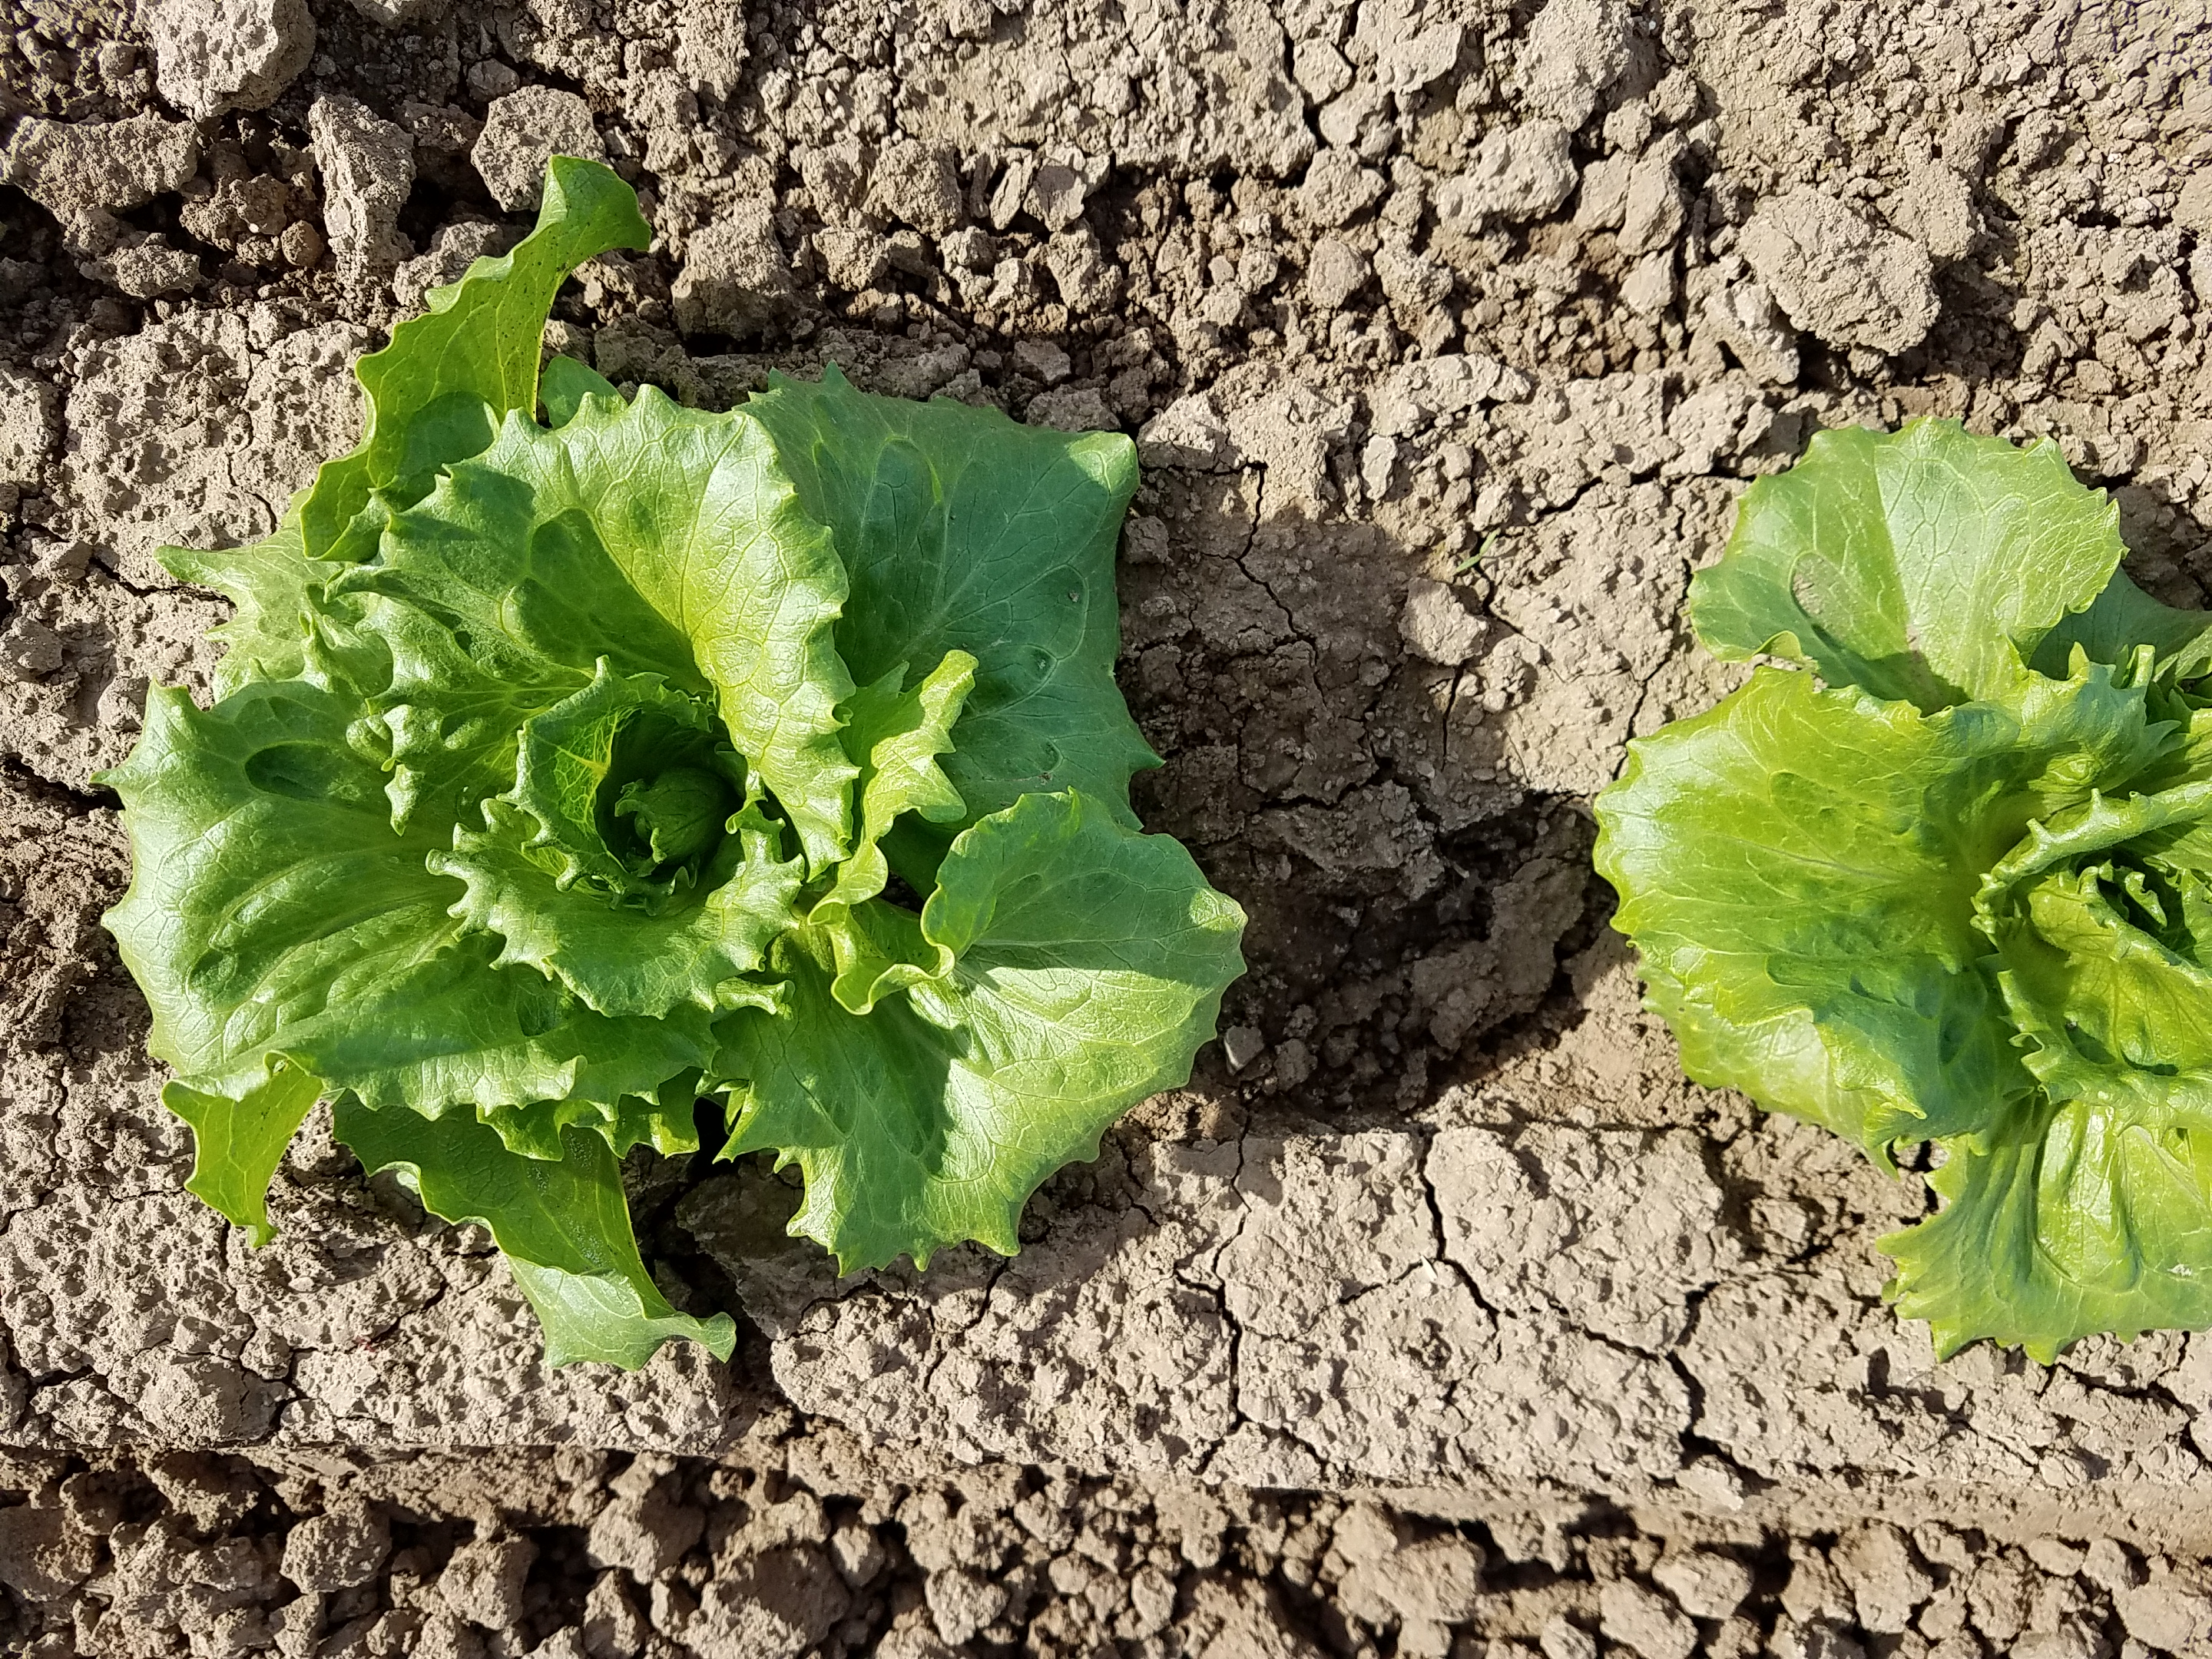
\includegraphics[width=1\linewidth]{./figures/problem-cutoff.jpg}
		\caption{The vegetation is cut off.}
		\label{fig:problem-cutoff}		
	\end{subfigure}%
	\caption[Common problems in field images]{These cases illustrate common problems encountered in image sets where the crop-line cannot be conclusively determined (\ref{fig:problem-cropline}) and the cutoff of vegetation (\ref{fig:problem-cutoff}). In the case where images contain a single image of crop the intended crop-line cannot be automatically determined. In the case where vegetation is cut off along the edges of the image shape analysis cannot be used, as otherwise the shape of the vegetation is distorted by the clean, straight edge. \textit{Source: Dr.~Mark Siemens, University of Arizona}}
\end{figure}



\subsection{Prepared Images}
The images acquired in the field are prepared using Adobe Photoshop\textsuperscript{\textregistered} to create test data for various scenarios:
\begin{itemize}
	\item{The presence of a specific weed in the image.}
	\item{While somewhat tangential to the task of classification, the presence of unwanted vegetation too close to wanted vegetation may lead to the same classification, but a different treatment. This is the case where vegetation is identified as \textit{undesired}, but is left untreated due to the risk of treatment would pose to the crop.} This is achieved in two ways -- duplicating or moving an existing weed within the image and inserting a new weed image obtained elsewhere.
	\item{Debris in the image -- this is the case where non-vegetated matter appears in the image. While the image segmentation discussed in section \ref{section:segmentation} should result in non-vegetated matter being removed, inserting both expected (irrigation equipment) and unexpected (human litter) into the images is a mechanism to test various scenarios.}
\end{itemize}

\begin{figure*}[h]
	\begin{subfigure}[t]{0.48\linewidth}
		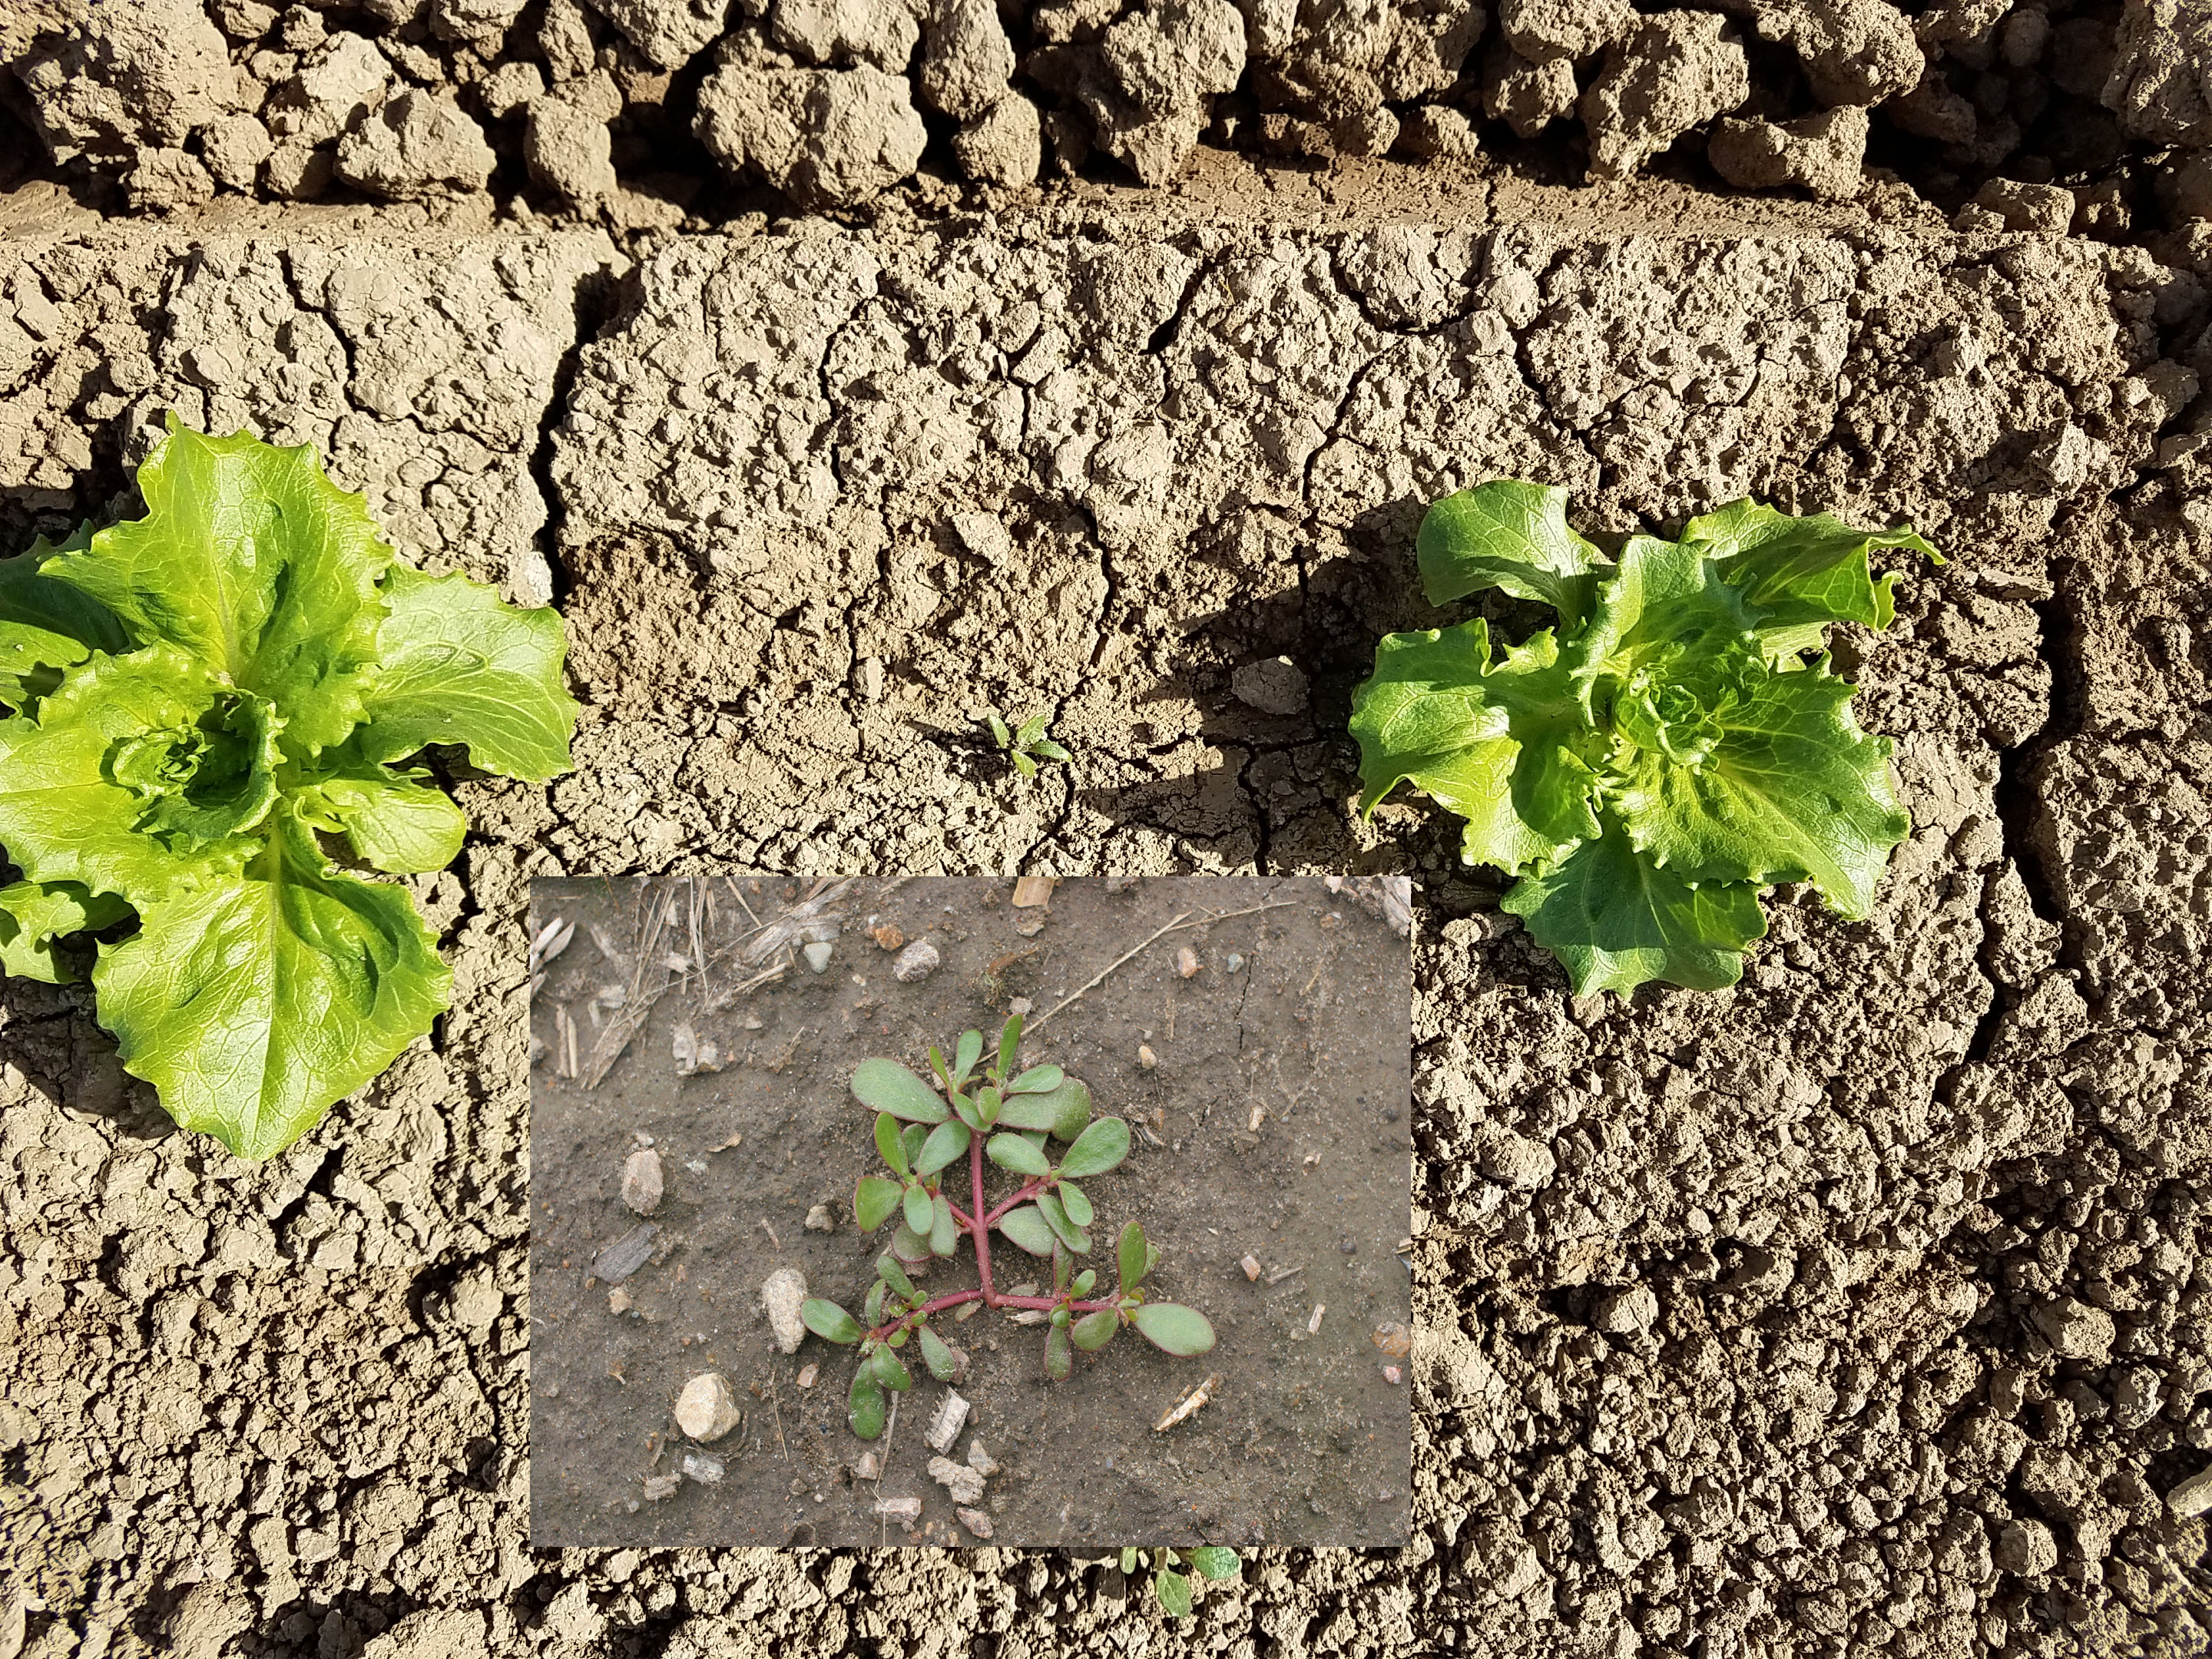
\includegraphics[width=1\linewidth]{./figures/with-purslane.jpg}
		\caption{Purslane (\textit Portulaca oleracea) inserted.}
		\label{fig:prepared-weed}
	\end{subfigure}
	\hfill
	%
	% TODO: Replace this image with one where irrigation equipment is inserted into image
	%
	\begin{subfigure}[t]{0.48\linewidth}
		\includegraphics[width=1\linewidth]{./figures/cantaloupe-with-lid.jpg}
		\caption{Identifying lid beside plant.}
		\label{fig:prepared-lid}		
	\end{subfigure}%
	\caption[Prepared images]{Images acquired in the field are subsequently manipulated by either inserting images of weeds not already present (\ref{fig:prepared-weed}), or inserting non-vegetated items (\ref{fig:prepared-lid}). Both cases are intended to present situations that should be handled by the classification algorithms. \\ \textit{Manipulated images: (\ref{fig:prepared-weed}) Dr. Mark Siemens, University of Arizona}}
\end{figure*}


Here, vegetation is placed within separate layers to create a composite image that shows the desired result.  Figure~\ref{fig:prepared-weed} illustrates the basic technique that is used to form a single image of both crop and a weed. This figure shows several differences that are immediately obvious: scale differences, as the weed image was obtained at a different distance, and lighting difference, as the weed image was obtained at a different location. Inserting a weed into an image solely for the purposes of classification has little value, of course, as classification of separate images is equivalent. The intent of this is to test the effect of the weed's proximity to the crop. Images are also manipulated to test certain scenarios, as Figure \ref{fig:prepared-lid} shows. A bucket lid with dots used to identify a specific plant is inserted into the image two test two things: the exclusion of the bucket lid itself, and the identification of the lid and plant it is closest to.


\section{Approach To Classification}
The goal of this processing flow is to determine what each item within the image is and classify it as desired or undesired. Weeds are, of course, undesired, but crop plants can also be classified as \textit{undesired} in the case of thinning operations, so this document will use the term \textit{undesired} and \textit{weed} interchangeably. Vegetation in an image falls into one of these classifications:
\begin{itemize}
	\item{Desired, the crop}
	\item{Undesired, weeds that can be treated without crop damage}
	\item{Unknown, vegetation that cannot be confidently identified}
	\item{Ignored, vegetation that is too close to desired vegetation to be treated without crop damage}
\end{itemize}

Additionally, this work makes a few simplifying assumptions about the images:
\begin{itemize}
	\item{Crop is typically in roughly alignment (the centers will be with a few degrees of each other).}
	\item{Weed centers are typically not in horizontal alignment.}
	\item{Crop is typically much larger than weeds.}
\end{itemize}

These are not without exceptions. For instance, a weed may be in perfect alignment within a crop line and two other plants. Each of these observations, however, are used in classification. Take, for instance, the observation that crop tends to be much larger than weeds. If the size of an item is three times that of another, the smaller item is -- more likely than not -- a weed. Another exception comes from orientation. Commonly encountered in images acquired with an automated platform, but less so with manually acquired ground images is that vegetation does not appear in horizontal or vertical orientation, complicating simplistic attempts to classify off-horizontal or off-vertical vegetation as weeds.

\begin{figure}[H]
	\centering
	\includegraphics[width=0.48\linewidth]{./figures/crop-alignment}
	\caption{Crop may not be in perfect horizontal or vertical alignment in images acquired autonomously. In this drone image, the crop is not in an alignment that would lend itself to crop identification in either orientation, as the crop-lines are along diagonals through the image.}
	\label{fig:alignment}	
\end{figure}

%\section {Study Area}
%This study will be carried out at the University of Arizona Maricopa Agricultural Center (MAC) on a cantaloupe crop (Spring 2024) and broccoli crop (Fall 2024) overseen by Drs. Attalah and Elshikha (University of Arizona), as part of another study.\footnote{The field in question is located at N 33.061805$^{\circ}$ W 111.966162$^{\circ}$} That study will involve three separate water treatments: center-pivot, flood irrigation, and drip. As the drip treatment study area is unlikely to produce a heavy weed load, it will not be included in this study, as differentiating between crop and weeds is an initial goal of this study. The study site is relatively free of obstacles that would impact low level flight with one notable exception: the center pivot irrigation system. Allowances will be made to avoid that system, but doing so is not expected to affect flight plans, as images in only subset of the field is planned to be captured.
 

\section{Software Environment \& Source code}
Both commercial and open-source software were used in the development an operational aspects of this study. While the majority of the software (the operational portions responsible for image processing and classification) was written in Python, commercial packages were used for pre-processing. Additionally, R was used in visualization and analysis of classification results. Some of these components play a large enough role that they warrant special mention in various places throughout this document, but in-depth descriptions of them will not be made here. Likewise, this list is not exhaustive, as numerous libraries were used for a few functions. The complete source code for this project is available in this GitHub repository: \href{https://github.com/evan-mcginnis/weeds}{\textit {weeds}}. Images, both raw and processed, are far too large to be hosted with GitHub, and are available on request from the author.

All development was done on Windows 10 and Ubuntu 18.04.06 with analysis on the University of Arizona's \textit{High Performance Compute Cluster}.

{
% This avoids the document line spacing affecting the contents of the table
\setstretch{1.0}
\begin{longtable}{x{\dimexpr.20\columnwidth-2\tabcolsep}
                  x{\dimexpr.20\columnwidth-2\tabcolsep}
                  x{\dimexpr.5\columnwidth-2\tabcolsep}}
%\begin{hyphenrules}{nohyphenation}
    \caption{Software Used}\label{tab:software}  \\
\toprule
{\textbf{Component}} & {\textbf{Use}} & {\textbf{Comment}}
\tabularnewline
\midrule
    \endfirsthead
%%%%
    \caption{Software Used (cont.)}\label{tab:software}  \\
\toprule
{\textbf{Component}} & {\textbf{Use}} & {\textbf{Comment}}
\tabularnewline
\midrule
    \endhead
%%%%
\midrule[\heavyrulewidth]
\multicolumn{3}{r}{\footnotesize\itshape
                   Continued on the next page}
    \endfoot
%%%%
\bottomrule
    \endlastfoot
%%%%
		PyCharm 
		& Python IDE     
		& Commercial software for Python development
\tabularnewline\addlinespace
		Python 3.9     
		& Python runtime                    
		& Most software was written in python
\tabularnewline\addlinespace
		scikit-learn
		& Machine Learning     
		& Implementations for various ML techniques 
\tabularnewline\addlinespace
		imbalance-learn
		& Class Imbalance     
		& Various imbalance correction techniques  
\tabularnewline\addlinespace
		OpenCV2 
		& Image Processing     
		& Machine Vision and Image Processing framework
\tabularnewline\addlinespace
		Numpy
		& Numeric Processing   
		& Python library
\tabularnewline\addlinespace
		Pandas 
		& Numeric Processing     
		& Python library
\tabularnewline\addlinespace
		PyQT5 
		& UI     
		& User Interface Framework for Python
\tabularnewline\addlinespace
		R 
		& Post Processing     
		& Statistical Software
\tabularnewline\addlinespace
		Plotly
		& Visualization     
		& Graphing libraries
\tabularnewline\addlinespace
		Adobe Lightroom
		& Color Correction     
		& Commercial software used for pre-processing
\tabularnewline\addlinespace
		Adobe Photoshop
		& Image preparation     
		& Commercial software used for image manipulation
\tabularnewline\addlinespace
		Dronelink
		& UAV Control     
		& Commercial software used for planning \& control
\tabularnewline\addlinespace
		MongoDB
		& Image organization     
		& No-SQL database 
\tabularnewline\addlinespace
		Docker Container
		& Virtualization     
		& Virtual containers host database and web server
\tabularnewline\addlinespace
		Slurm
		& Workload     
		& Supercomputer workload management
\label{table:software}
\end{longtable}
}

Minor use was made of C++ (a compiled language) and PyCuda, a library allowing access to a GPU when exploring performance improvements, but  that use was not key to the findings presented here.

\section{Workflow}
Images are processed following the workflow shown in Figure~\ref{fig:workflow}. Each step in this workflow will be discussed in subsequent sections. The images that appear in subsequent sections are just to illustrate concepts, and are not included in the final analysis.\footnote{The example images and analysis within the next few sections are taken from a set of images supplied by Dr. Mark Siemens, University of Arizona, and as such are not expected to provide an exact match to those acquired under the field conditions of this study. These images, however, are useful in the demonstration of key techniques. This image set of 39 images was taken in 2019 with a Samsung SM-G930V phone.} The workflow illustrated supports the notion of supervised learning, where a human classifies plants that are then used in a model for predicting the plant's class. That is, the two workflows are identical, with the sole difference being that a model replaces the human in classification. 
\begin{figure}[H]
	\centering
	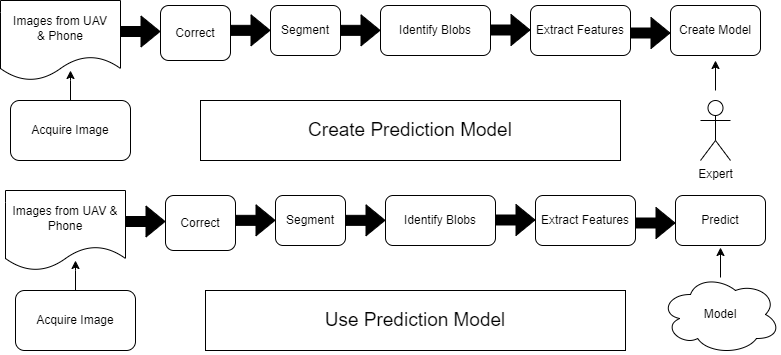
\includegraphics[width=0.85\linewidth]{./figures/workflow.png}
	\caption{Image processing workflow. There are two workflows followed, the creation of the model (where a human classifies the vegetation in the image) and use of that model to predict the plant.}
	\label{fig:workflow}	
\end{figure}


\section{Acquire Image}
Image acquisitions were carried out at the Maricopa Agricultural Center (MAC) on a cantaloupe planting (N $33.061857^\circ$, E $111.967145^\circ$) consisting of 3 water treatments: flood, drip, and center-pivot, each watered at 80\% and 100\%. Only the flood and pivot treatments will be imaged and considered for this study. This is mostly motivated by practical considerations: it is not anticipated that the drip treatment plots will have a significant number of weeds.  Image acquisition will take place on at regular intervals beginning in April 2024 and continuing through May 2024 (Cantaloupe), and October 2024 continuing through November 2024 (Broccoli).  Ambient lighting conditions in acquisitions were quite similar, as they were carried out around the same time (mid-morning) and under (almost) cloudless skies.

Images were captured at several distances AGL: 20cm, 1m, 2m, 5m.

With the exception of images taken from 20cm, all images were acquired using a DJI Mavic Air 2S with a stock RGB 20 MP sensor. The UAV camera has the following relevant details:

\begin{itemize}
	\item{13.25mm sensor width}
	\item{8.38mm focal length}
	\item{5464 pixel width}
	\item{3640 pixel height}
\end{itemize}

Images gathered at 20cm were taken with an iPhone 14 Pro, using the 48MP main camera.

\begin{itemize}
	\item{7.3mm sensor width}
	\item{8.38mm focal length}
	\item{8063 pixel width}
	\item{6048 pixel height}
\end{itemize}

It is fair to characterize the drone flight altitude as unrealistically low. This is mostly pragmatic, as the UAV was treated more as a flying camera that allowed images to be acquired shortly after irrigation, and avoided requiring entering the field even when conditions allowed.  Perhaps just as importantly for this study was confirming ground truth of a vegetation class. The class of a plant could be manually confirmed at 2 meters, but those from higher altitudes could not be. Other pragmatic concerns must also be considered. UAVs can acquire images in situations where ground acquisition (towed, self-propelled, or even a phone camera on a stick) are infeasible due to field conditions (after an irrigation or precipitation). In any event, there is nothing about this study that is specific to UAVs.


Each image acquisition activity was accompanied by an image of a \href{https://www.datacolor.com/spyder/products/spyder-checkr-photo/} {SpyderChecker 24} color calibration chart (under the same ambient lighting conditions) and color correction was subsequently applied using Adobe Photoshop Lightroom Classic and custom calibration profiles created using the Spyder Checkr software. Raw sensor data from both camera systems was stored in Adobe Digital Negative (DNG) format before color correction and conversion to a compressed JPG format for the resulting images. The digital negative of each image (DNG, a standard format for raw sensor data) was corrected and converted to JPG format for subsequent processing.\footnote{The merits of raw, uncompressed, and unprocessed sensor data versus compressed, processed formats like JPG are beyond the scope of this document, but it is fair to say taking raw sensor data, processing, and then producing a compressed JPG is precisely what consumer products like phone cameras do. So that the color correction step can be inserted, the process of producing an image that can be viewed with most software is altered a bit, but essentially unchanged. A picture stored as a DNG is not higher resolution or higher quality than a JPG equivalent, just more easily manipulated without the introduction of errors. That is, JPG is simply a commonly encountered format for images that is considerably smaller than what would be expected of raw sensor data.} The sensor data for each image was quite large, requiring 38.5 MB of storage, with equivalent JPG images much smaller.
Where feasible, missions were conducted in the same ambient light conditions, but an exact match of ambient conditions using uncontrolled lighting is not always possible. As all missions took place in mid-morning under cloudless skies, the resulting image sets are fairly closely matched in terms of illumination and color temperature.

%
% I M A G E  S E G M E N T A T I O N
%
\section{Segment Image}
\label{section:segmentation}
Perhaps the least compute-intensive portion of this workflow is simply to discard to portion of an image that does not contribute meaningfully to classification, and for this problem space those pixels that do not contribute useful information are, most notably, pixels representing the ground. There are three segmentation approaches considered for this task: index-based, threshold based, and deep-learning based. The result of each of these approaches is the same: the portions of the images that did not contain pixels with vegetation present were the discarded by creating a mask using one of the techniques and applying that mask to the original image to both isolate the vegetation and reduce the information content. This discards both the ground and debris while retaining the vegetation. 

\subsection{RGB Index Based}
These images were segmented using various visible light indices (\cite{Hunt2013-ih}, \cite{Hamuda2016-dw}). As this process is not the primary subject of this paper, it will be given only superficial mention here.  Various approaches to image segmentation are  summarized in Table \ref{table:segmentation}.  The intent of this step of the workflow is not to classify the individual plants, but to preprocess the image before further analysis is done.

{\renewcommand{\arraystretch}{2}%

{
% This avoids the document line spacing affecting the contents of the table
\setstretch{1.0}
% Example to span two pages
\begin{longtable}{x{\dimexpr.25\columnwidth-2\tabcolsep}
                  x{\dimexpr.35\columnwidth-2\tabcolsep}
                  x{\dimexpr.4\columnwidth-2\tabcolsep}}
%\begin{hyphenrules}{nohyphenation}
    \caption{Visible light indices}\label{tab:example}  \\
\toprule
{\textbf{Index}} & {\textbf{Formula}} & {\textbf{Comment}}
\tabularnewline
\midrule
    \endfirsthead
%%%%
    \caption{Visible light indices (cont.)}\label{tab:example}  \\
\toprule
{\textbf{Index}} & {\textbf{Formula}} & {\textbf{Comment}}
\tabularnewline
\midrule
    \endhead
%%%%
\midrule[\heavyrulewidth]
\multicolumn{3}{r}{\footnotesize\itshape
                   Continued on the next page}
    \endfoot
%%%%
\bottomrule
    \endlastfoot
%%%%
		Triangular Greenness
		& \begin{minipage}[t]{0.3\textwidth}
			$R_{green} - \alpha R_{red} - \beta R_{blue}\\ \alpha = \frac {2(\lambda_{blue} - \lambda_{green})} {(\lambda_{blue} - \lambda_{red})}\\ 
		    	\beta = \frac {2(\lambda_{green} - \lambda_{red})} {(\lambda_{blue} - \lambda_{red})} $
		   \end{minipage}     
		& Corrects for camera calibration using the peak sensitivity
\tabularnewline\addlinespace

		Normalized Difference     
		& $128 * \left( \left( \frac {(G - R)} {(G + R)} \right) + 1 \right) $                    
		& The NDI index produces a near-binary image. 
\tabularnewline\addlinespace

		Excess Green      
		& \begin{minipage}[t]{0.3\textwidth}
			$R = \frac {R} {R_{max}}\\ G = \frac {G} {G_{max}}\\ B = \frac {B} {B_{max}}$ 
		   \end{minipage}
		& ExG provided a clear contrast between plants and soil 
\tabularnewline\addlinespace

		Excess Red      
		& $1.3 R - G$ 
		& inspired by the fact that there are 4\% blue, and 32\% green, compared with 64\% red cones in the retina of the human eye
\tabularnewline\addlinespace

		Color Index of Vegetation Extraction      
		& $0.441 R - 0.811 G + 0.385 B + 18.78745$
		& This method was proposed to separate green plants from soil background in order to evaluate the crop growing status.
\tabularnewline\addlinespace

		Excess Green - Excess Red   
		& $ExG - ExR$ 
		& ExG used to extract the plant region and ExR used to eliminate the background noise (soil and residue) where green–red material (stems, branches, or petioles) may exist
\tabularnewline\addlinespace

		Normalized Green-Red Difference    
		& $\frac {(G - R)} {(G + R)}$ 
		& The method of NGRDI was used to overcome the differences in exposure settings selected by the digital camera when acquiring aerial photography of the field. 
\tabularnewline\addlinespace

		Vegetative Index      
		& $\frac {G} {R^aB^{(1-a)}}, a = 0.667$ 
		& VEG has a significant advantage because it is robust to lighting change.
\tabularnewline\addlinespace

		Com1   
		& $ExG + CIVE + ExGR + VEG$ 
		& High computational cost --- does not perform well in high or low light levels
\tabularnewline\addlinespace

		Modified Excess Green      
		& $1.262G - 0.884R = 0.311B$ 
		& Does not perform well in high or low light levels. 
\tabularnewline\addlinespace

		Combined Indices 2      
		& $0.36ExG + 0.47CIVE + 0.17VEG$ 
		& Uses weighting factors to emphasize strengths of various approaches
%\tabularnewline\addlinespace
\label{table:indices}
\end{longtable}
}

These indices are used to create a mask that is then applied to the original source image to permit vegetation to show while masking details that are not relevant (ground pixels, stones, and other items that may appear in field conditions such as irrigation equipment) The intent here is to remove all pixels that are not relevant to the task of distinguishing between crop and weed while leaving the vegetated pixels unmanipulated.

\begin{figure}[H]
	\centering
	\begin{subfigure}[h]{.30\textwidth}
	  \centering
	  \includegraphics[width=1\linewidth]{figures/original.jpg}
	  \caption{Field view of lettuce and weed}
	  \label{fig:original}
	\end{subfigure}
	\begin{subfigure}[h]{.30\textwidth}
	  \centering
	  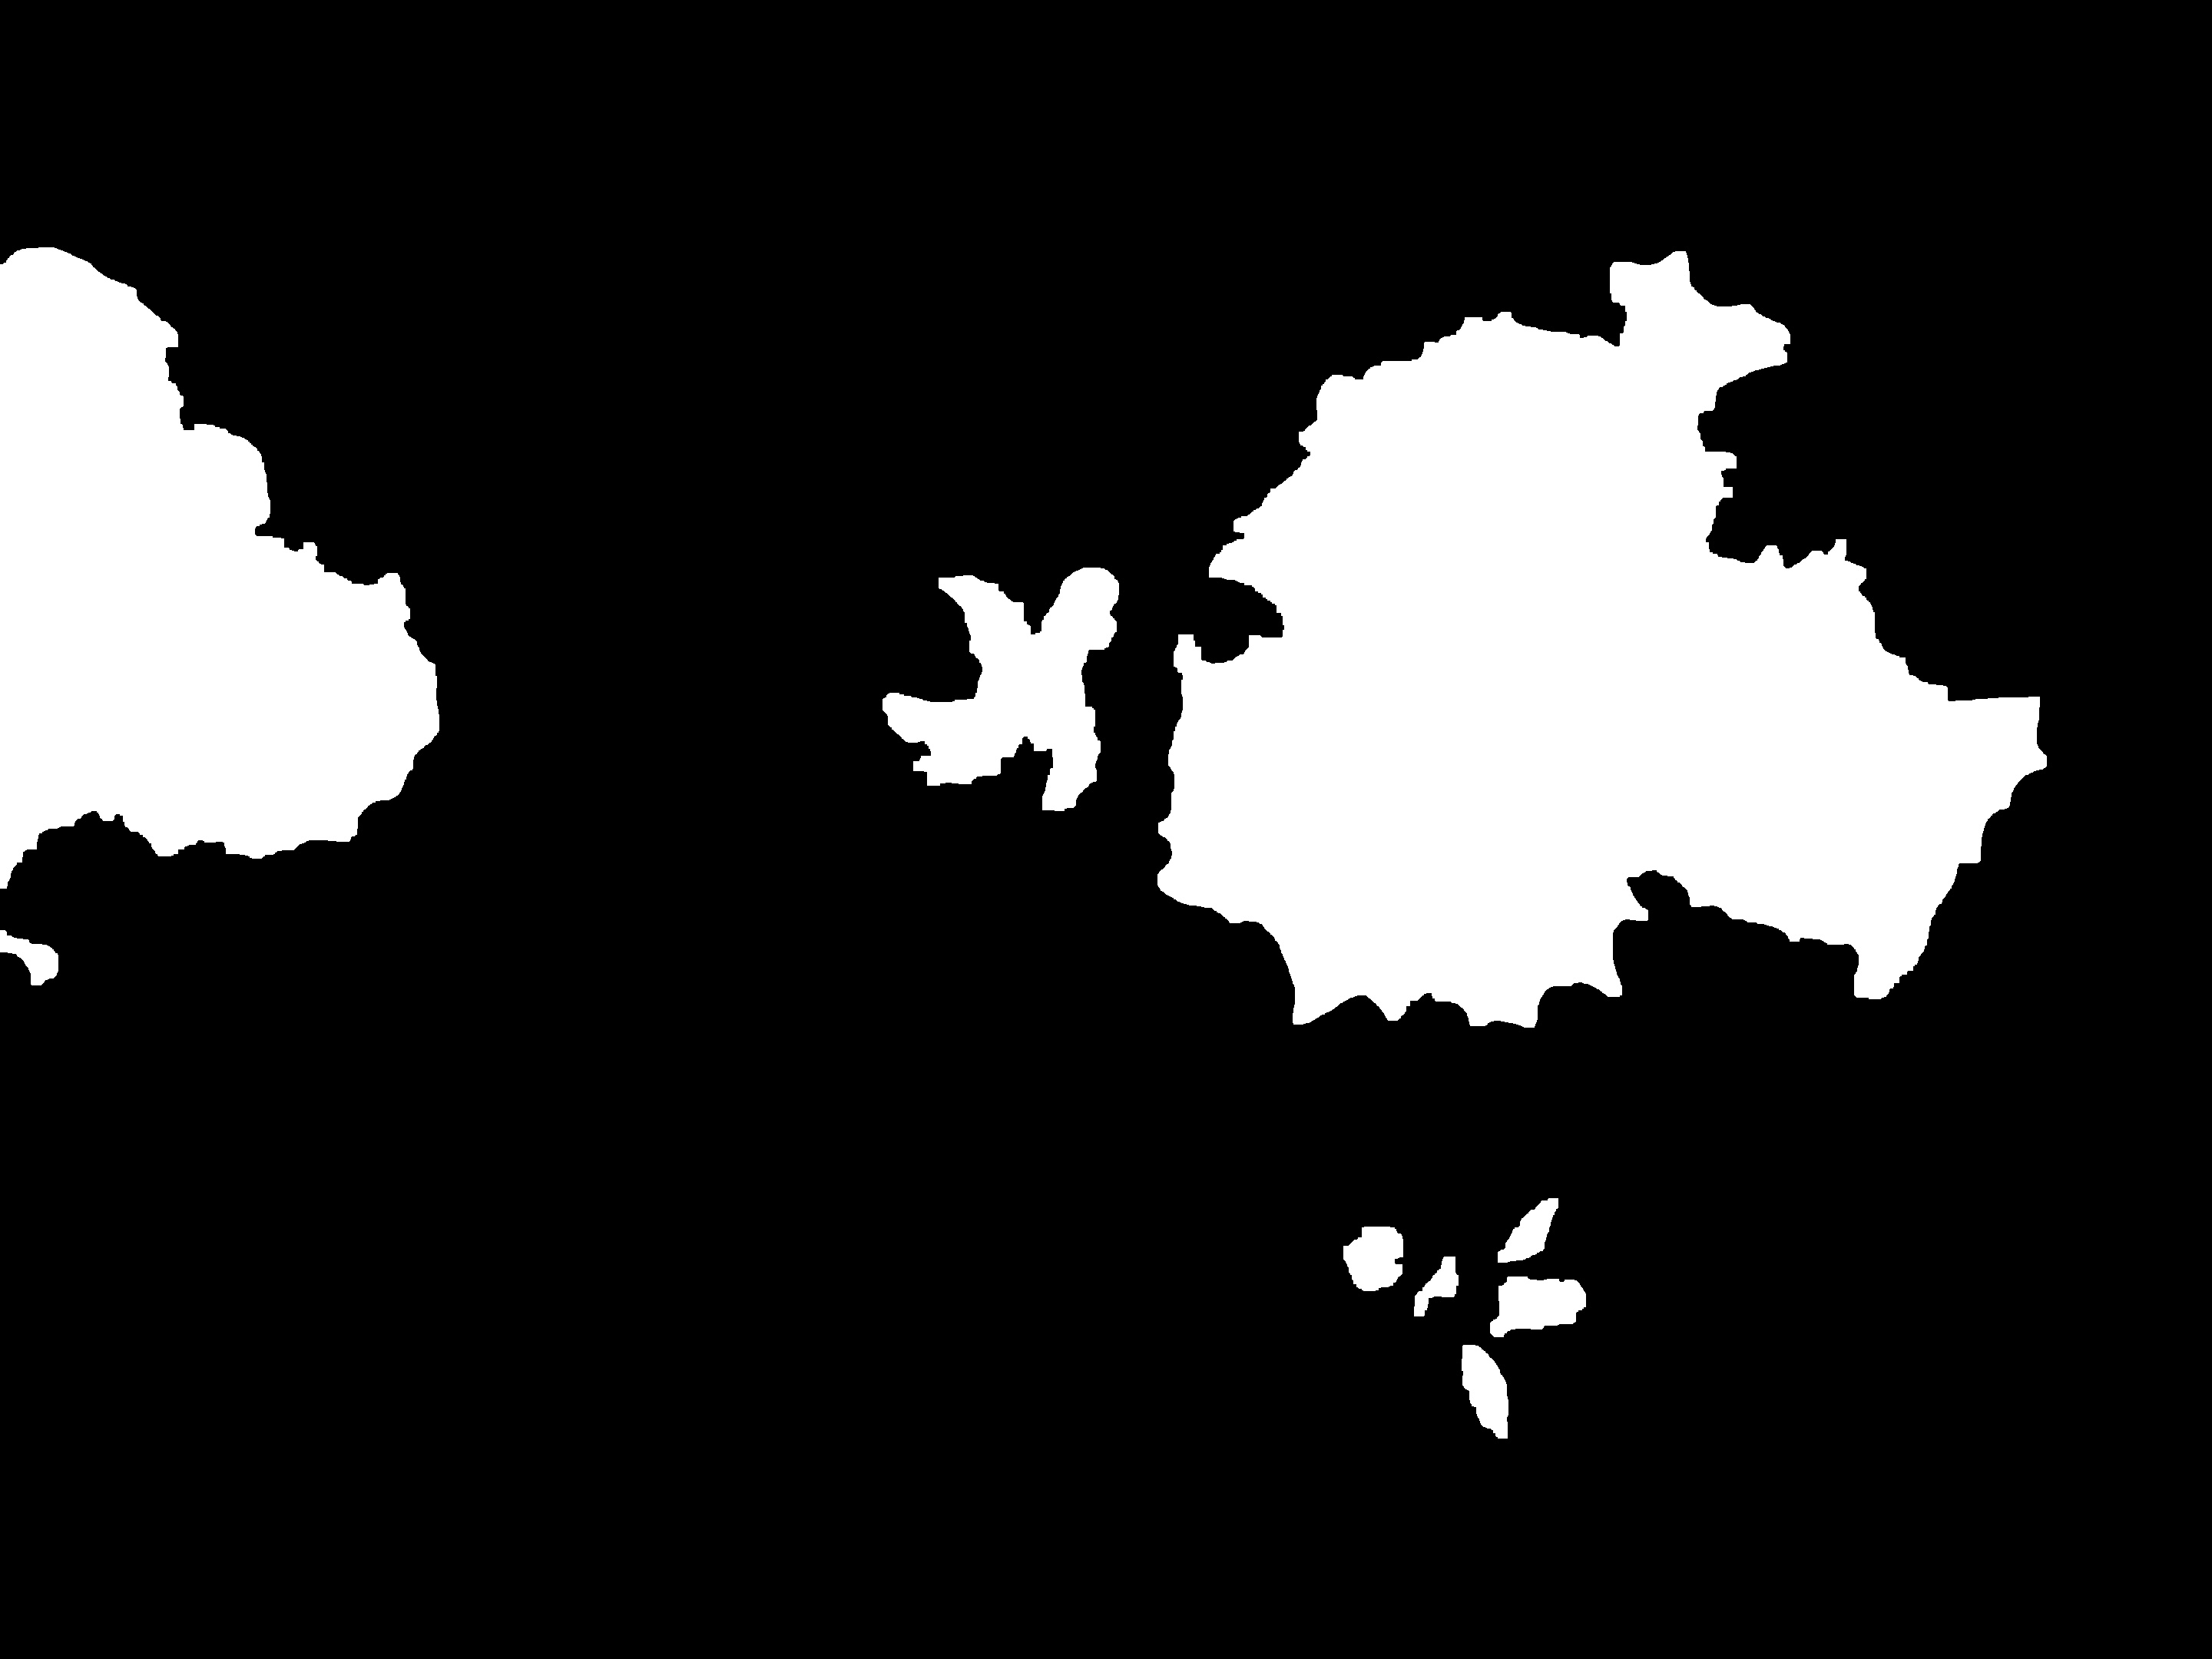
\includegraphics[width=1\linewidth]{figures/original-mask.jpg}
	  \caption{Mask produced with NDI}
	  \label{fig:mask}
	\end{subfigure}
	\begin{subfigure}[h]{.30\textwidth}
	  \centering
	  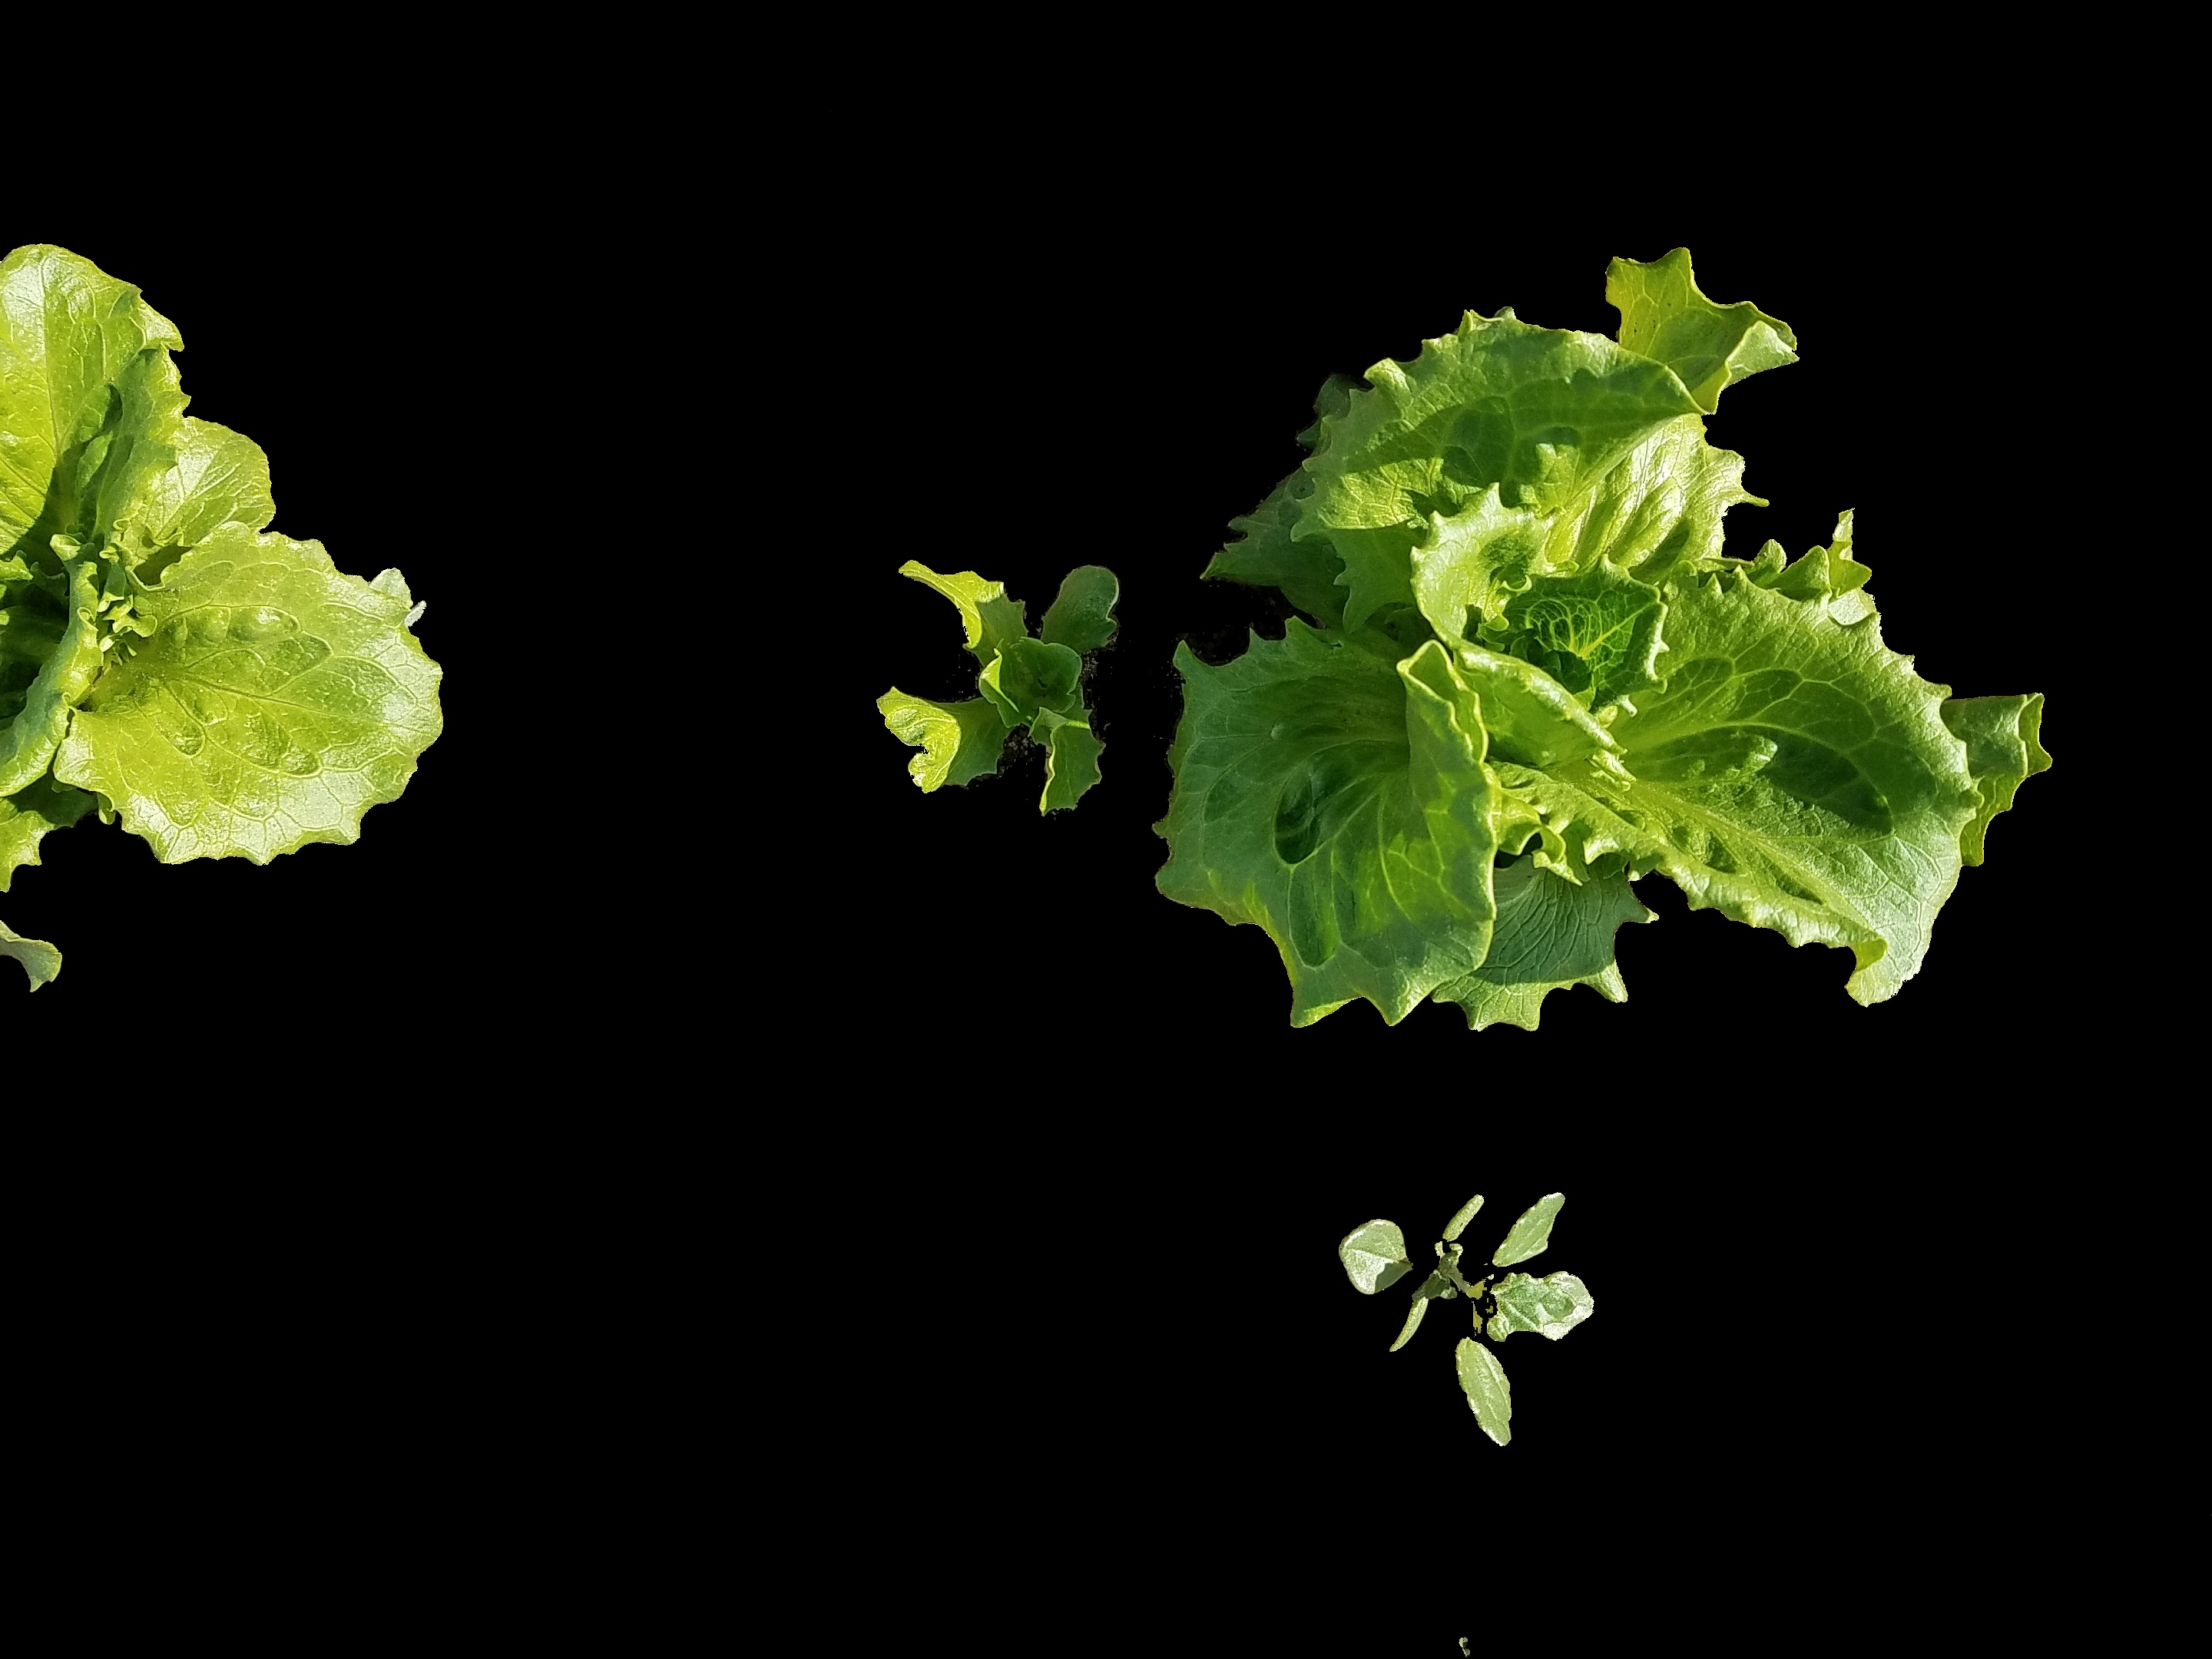
\includegraphics[width=1\linewidth]{figures/original-masked.jpg}
	  \caption{After applying mask}
	  \label{fig:original-masked}
	\end{subfigure}
	\caption[Before and after segmentation]{Before and after segmentation. Note the absence of the stems seen in the weed in the lower portion of~\ref{fig:original-masked} -- this is made a bit more obvious with a close examination of the mask shown in~\ref{fig:mask}. The lack of stems will lead to a single plant being identified as multiple plants, but does not affect shape-independent features such as texture and color, but will affect shapes, as will be discussed further in the section detailing problems (Section \ref{section:problems-color}).}
	\label{fig:segmentation}
\end{figure}
The segmented image has discarded ground pixels while retaining most of the pixels that will be used, but a close examination reveals that pixels in the stems of the weed are also eliminated, as they are less green than the rest of the plant. This effect is even more pronounced when segmenting images of weed that do not contain green stems as would be seen in the red stems seen in \textit{Portulaca oleracea} (Purslane). While they are not eliminated, pixels in the area of the deep shadows of the vegetation may affect attempts to classify objects based on color attributes. Unfortunately, the band of color featured in the stems (red) is frequently found in the background (soil), so attempts to make the stems appear in the masked image are problematic, as this solution tends to bring allow unwanted ground pixels in the final image that contain hues found within the stems. Likewise, immature vegetation where stems are not sufficiently green will not appear in the final image. Fortunately, both of these cases do not appear to have an appreciable effect on the classification. For the purposes of this paper, images will use the \textit{Normalized Difference Index} (NDI) segmentation approach (see Table~\ref{table:segmentation} for this formula). This process results in image data with only two sets of values: RGB values of zero where there is no vegetation and the original RGB values for pixels containing vegetation. Figure~\ref{fig:ndi-segmentation} illustrates the values used in producing a mask, but here we see a problem that must be solved: threshold selection.

The creation of an index has produced data that often exaggerates portions of the image with vegetated pixels, but deciding what portions of the data to discard and which to keep can be automated instead of using a single threshold for all images. The manual selection of a threshold can be shown to work relatively well, and can be fine-tuned by examining the results ensure that the number of vegetated pixels are maximized, while the number of non-vegetated pixels are minimized (in other words, we do not want to have significant portions of the ground in the image, but we do want as much of the plant as is possible). Unfortunately, images can be acquired under different lighting conditions, leading to the case where there is often not a threshold that works well for all images. An alternative, first proposed by \citeauthor{Otsu1979-io}  \cite{Otsu1979-io}, is to select this threshold automatically for each image, or the image can be selected using the \textit{Triangle} algorithm. Otsu's algorithm arrives at a threshold by maximizing the variance between foreground and background pixels. The triangle method arrives at a threshold as the point where a line connecting the histogram’s peak to the maximum intensity is maximized. Both of these techniques operate on greyscale images, considering only pixel intensity. It is also worth considering the distribution of pixel values: typically bi-modal (two distinct peaks) and unimodal (a single peak).

%
% Histogram produced with this command:'
% python plot-threshold.py -i d:\maricopa-test\flood-2-2m\DJI_0610.jpg

\begin{figure*}[h]
	\centering
	  	\subfloat[Intensity Histogram\centering]{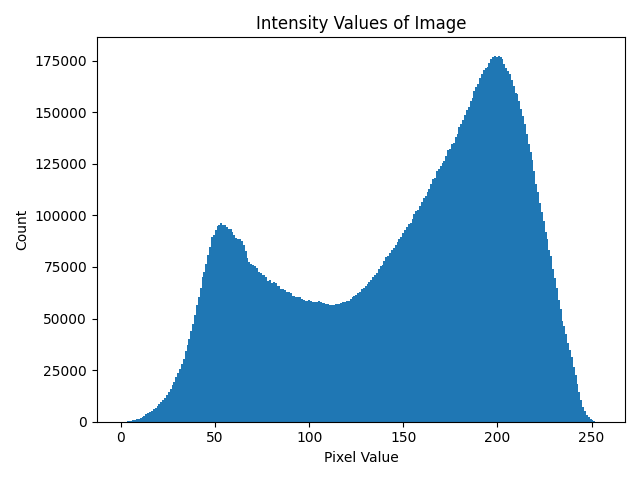
\includegraphics[height=0.19\textheight]{figures/pixel-values.png}\label{fig:intensity-histogram}}
		\hfil
	   	\subfloat[Source Image\centering]{\includegraphics[height=0.19\textheight]{figures/pixel-values-image.jpg}
	  \label{fig:source-image}}
	\caption[Bimodal distribution of pixel intensity]{A example of a bimodal distribution of pixel intensity values. Note that there are two peaks in the histogram above (\ref{fig:intensity-histogram}), corresponding to what can be observed in \ref{fig:source-image}, where there are only two classes of pixels visible: crop and ground.}
	\label{fig:intensity}
\end{figure*}

Otsu's method operates on the assumption that there are two classes of pixels in the object (interesting and uninteresting things). The algorithm minimizes intra-class variance. This method performs well when presented with images that have two distinct peaks.

% Equation from https://infoaryan.com/blog/opencv-python-otsu-and-triangle-thresholding-full-mathematics-code-explained-important/
\begin{equation}
\sigma^2_B (t) \times p(t) \times p(\overline{t}) \\
\end{equation}
where $\sigma^2_B (t)$ is the variance between the two classes, $p(t)$ is the probability of class $t$, and $p(\overline{t})$ is the probability of the complement.

For the triangle method uses this equation:
\begin{equation}
T_{triangle} = argmax \left[ h(T) \times \left( 1 - \left| \frac{T - P}{R - P} \right| \right) \right]
\end{equation}
Where $h(T)$ is the value at $T$, $R$ is the maximum of the intensity, and $P$ is the peak value. The triangle method often performs better than does Otsu's method when the pixel intensities exhibit a unimodal peak.

The details of the implementation of these two approaches are beyond the scope of this document, and while there are certainly others, these are, perhaps the most frequently encountered approaches. Both of these approaches, however, are based on some assumptions about the intensity histogram, and may not work well in all situations, particularly if these assumptions are not valid. Otsu's algorithm, for example, tends to yield satisfactory results when operating on images possessing a bimodal distribution, but may not yield good results on images with a single peak or multiple peaks.

\begin{figure}[h!]
	\centering
	\begin{subfigure}[h]{.48\textwidth}
	  \centering
	  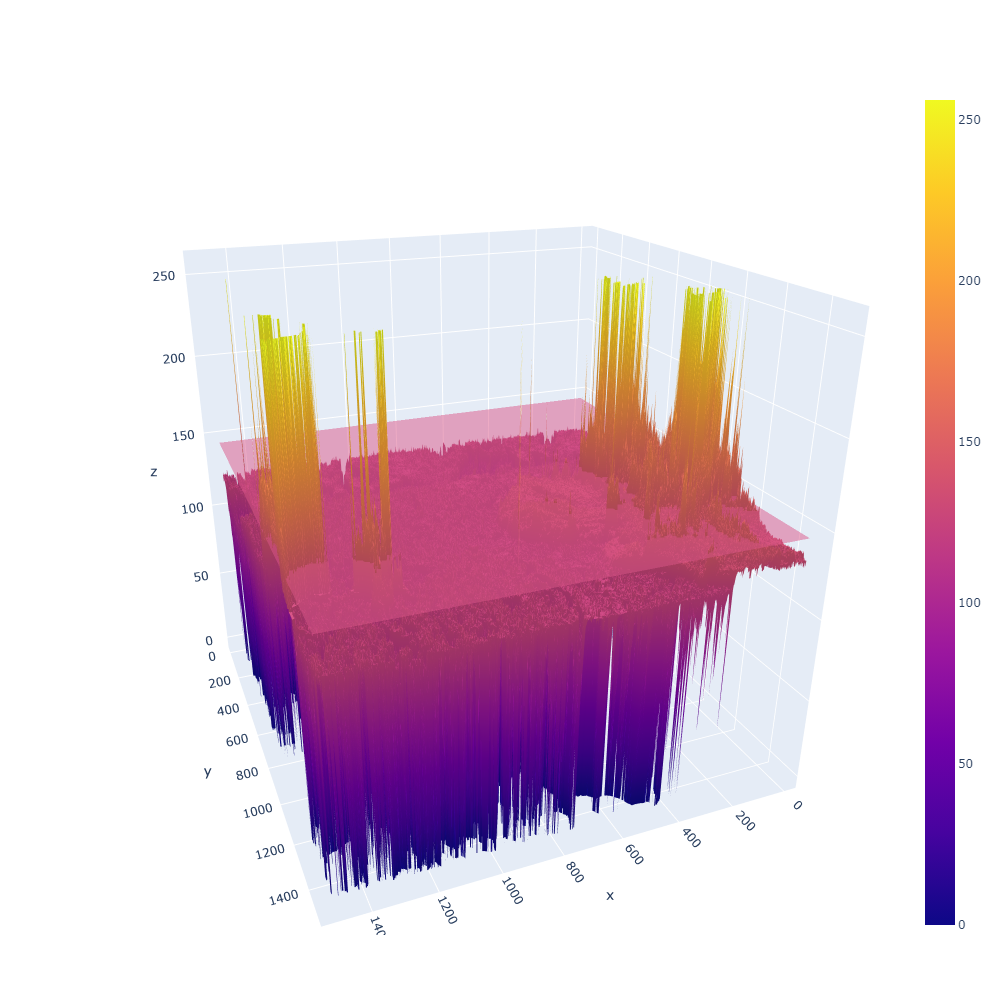
\includegraphics[height=5cm]{./figures/ndi-1-of-2.png}
	  \caption{Image segmented using NDI}
	  \label{fig:ndi-1}
	\end{subfigure}
	\hfil
	\begin{subfigure}[h]{.48\textwidth}
	  \centering
	  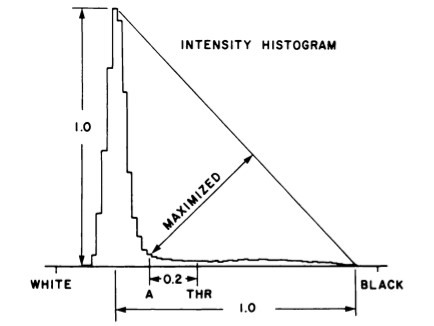
\includegraphics[height=5cm]{./figures/triangle-algorithm}
	  \caption{Triangle method for threshold selection.}
	  \label{fig:ndi-2}
	\end{subfigure}
	\caption[NDI segmentation and threshold selection]{An example of NDI segmentation and threshold selection. A threshold for the production of a mask can be done manually, perhaps by selecting all values below 140 to form the mask that will be applied to the image, illustrated by the semi-opaque plane. While that manual selection may be sufficient to perform the segmentation of an image set acquired under the same ambient conditions, it may lead to the exclusion of portions of the plant in images taken under different conditions. Using the \textit{Triangle} algorithm \parencite{Brink1996-xy,Zack1977-yl} allows this selection to be made automatically. The point at which the line between the lowest and highest points in the histogram is selected as the threshold, selecting a threshold applicable to each image in a set rather than a global value used for all images in a set.}
	\label{fig:ndi-segmentation}
\end{figure}

Visible light indices have a distinct advantage over other segmentation techniques for one very important reason: they are computationally cheap. While they involve as many calculations as there are pixels in the image, the number is relatively small. Given than compute resources may be limited in real-time systems operating under field conditions, this aspect may be an important factor worthy of consideration, particularly when a CPU is not dedicated to the imaging system. While the index calculation will benefit from performing these calculations on a GPU, a detailed analysis of the benefit of doing so is not detailed here, but is discussed in the section on performance (Section \ref{section:performance}).

Figure \ref{figure:results} shows the results of applying the masks to a image containing both ground and vegetation.

\begin{figure}[H]
\centering
\captionsetup[subfloat]{labelfont=scriptsize,textfont=scriptsize}
\begin{tabular}{cccccc}
\subfloat[NDI]{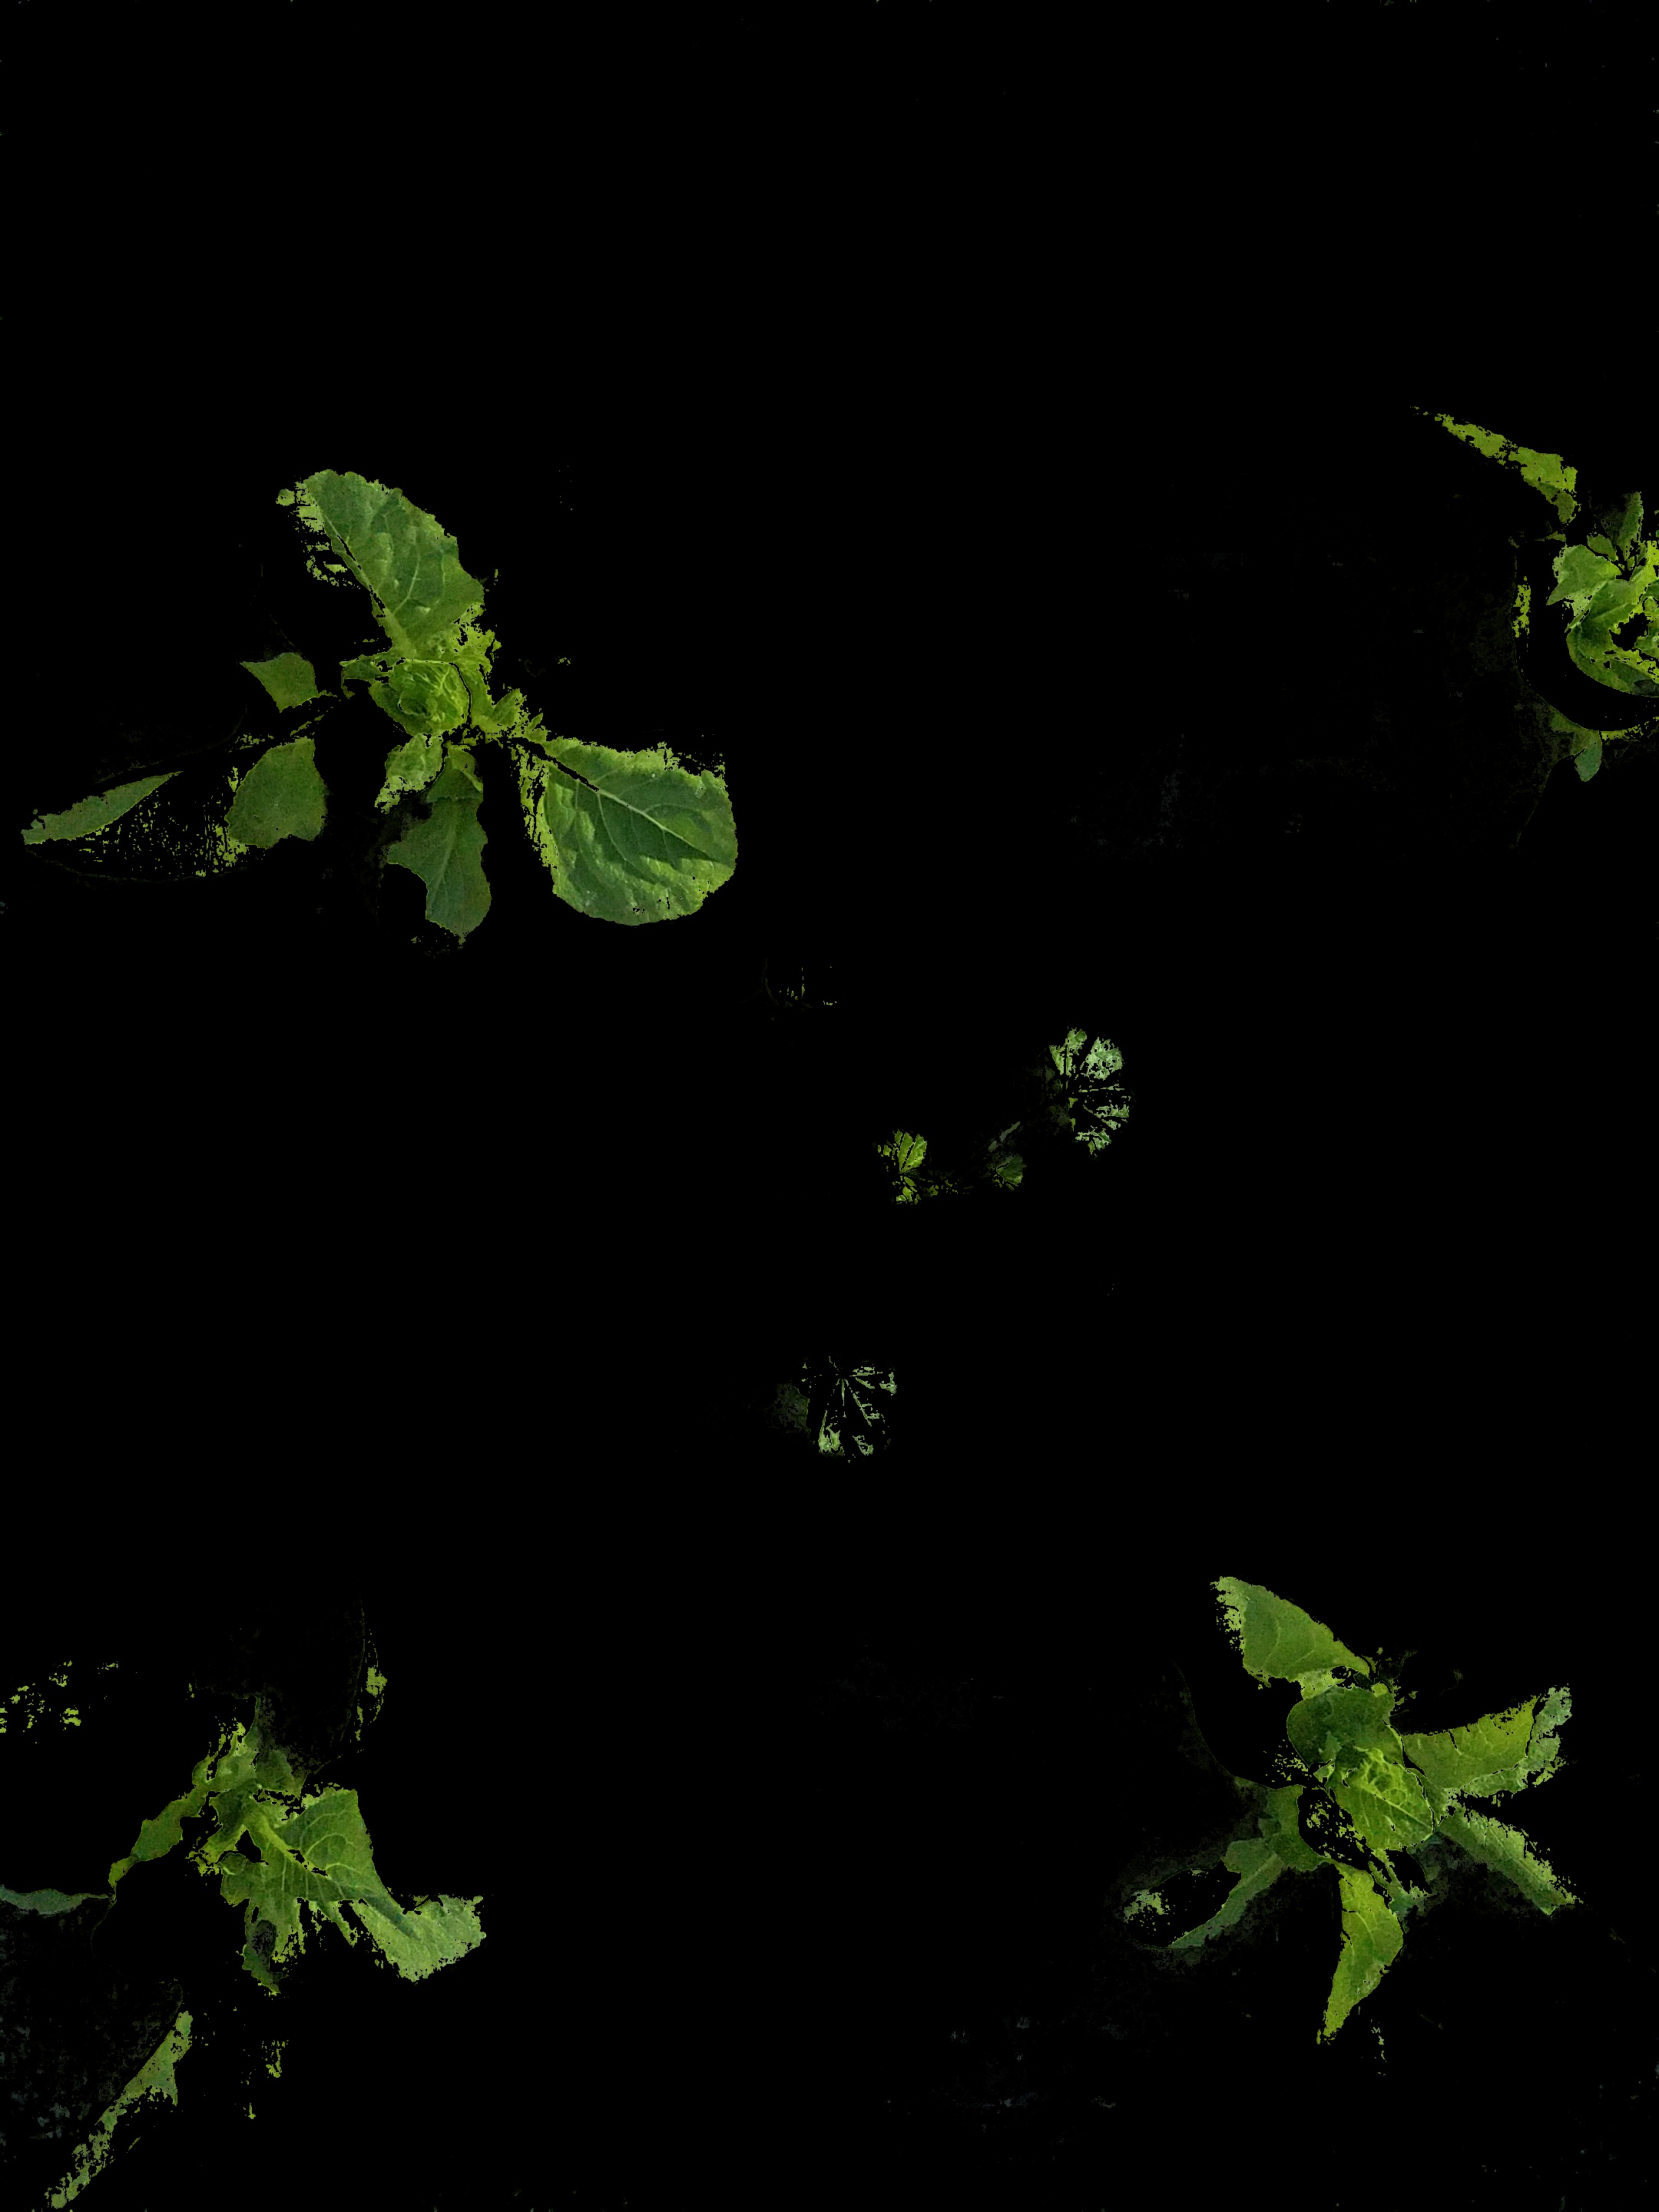
\includegraphics[height=0.10\textheight]{figures/20201117_112624-NDI.jpg} \label{fig:ndi}} &
\subfloat[EXG]{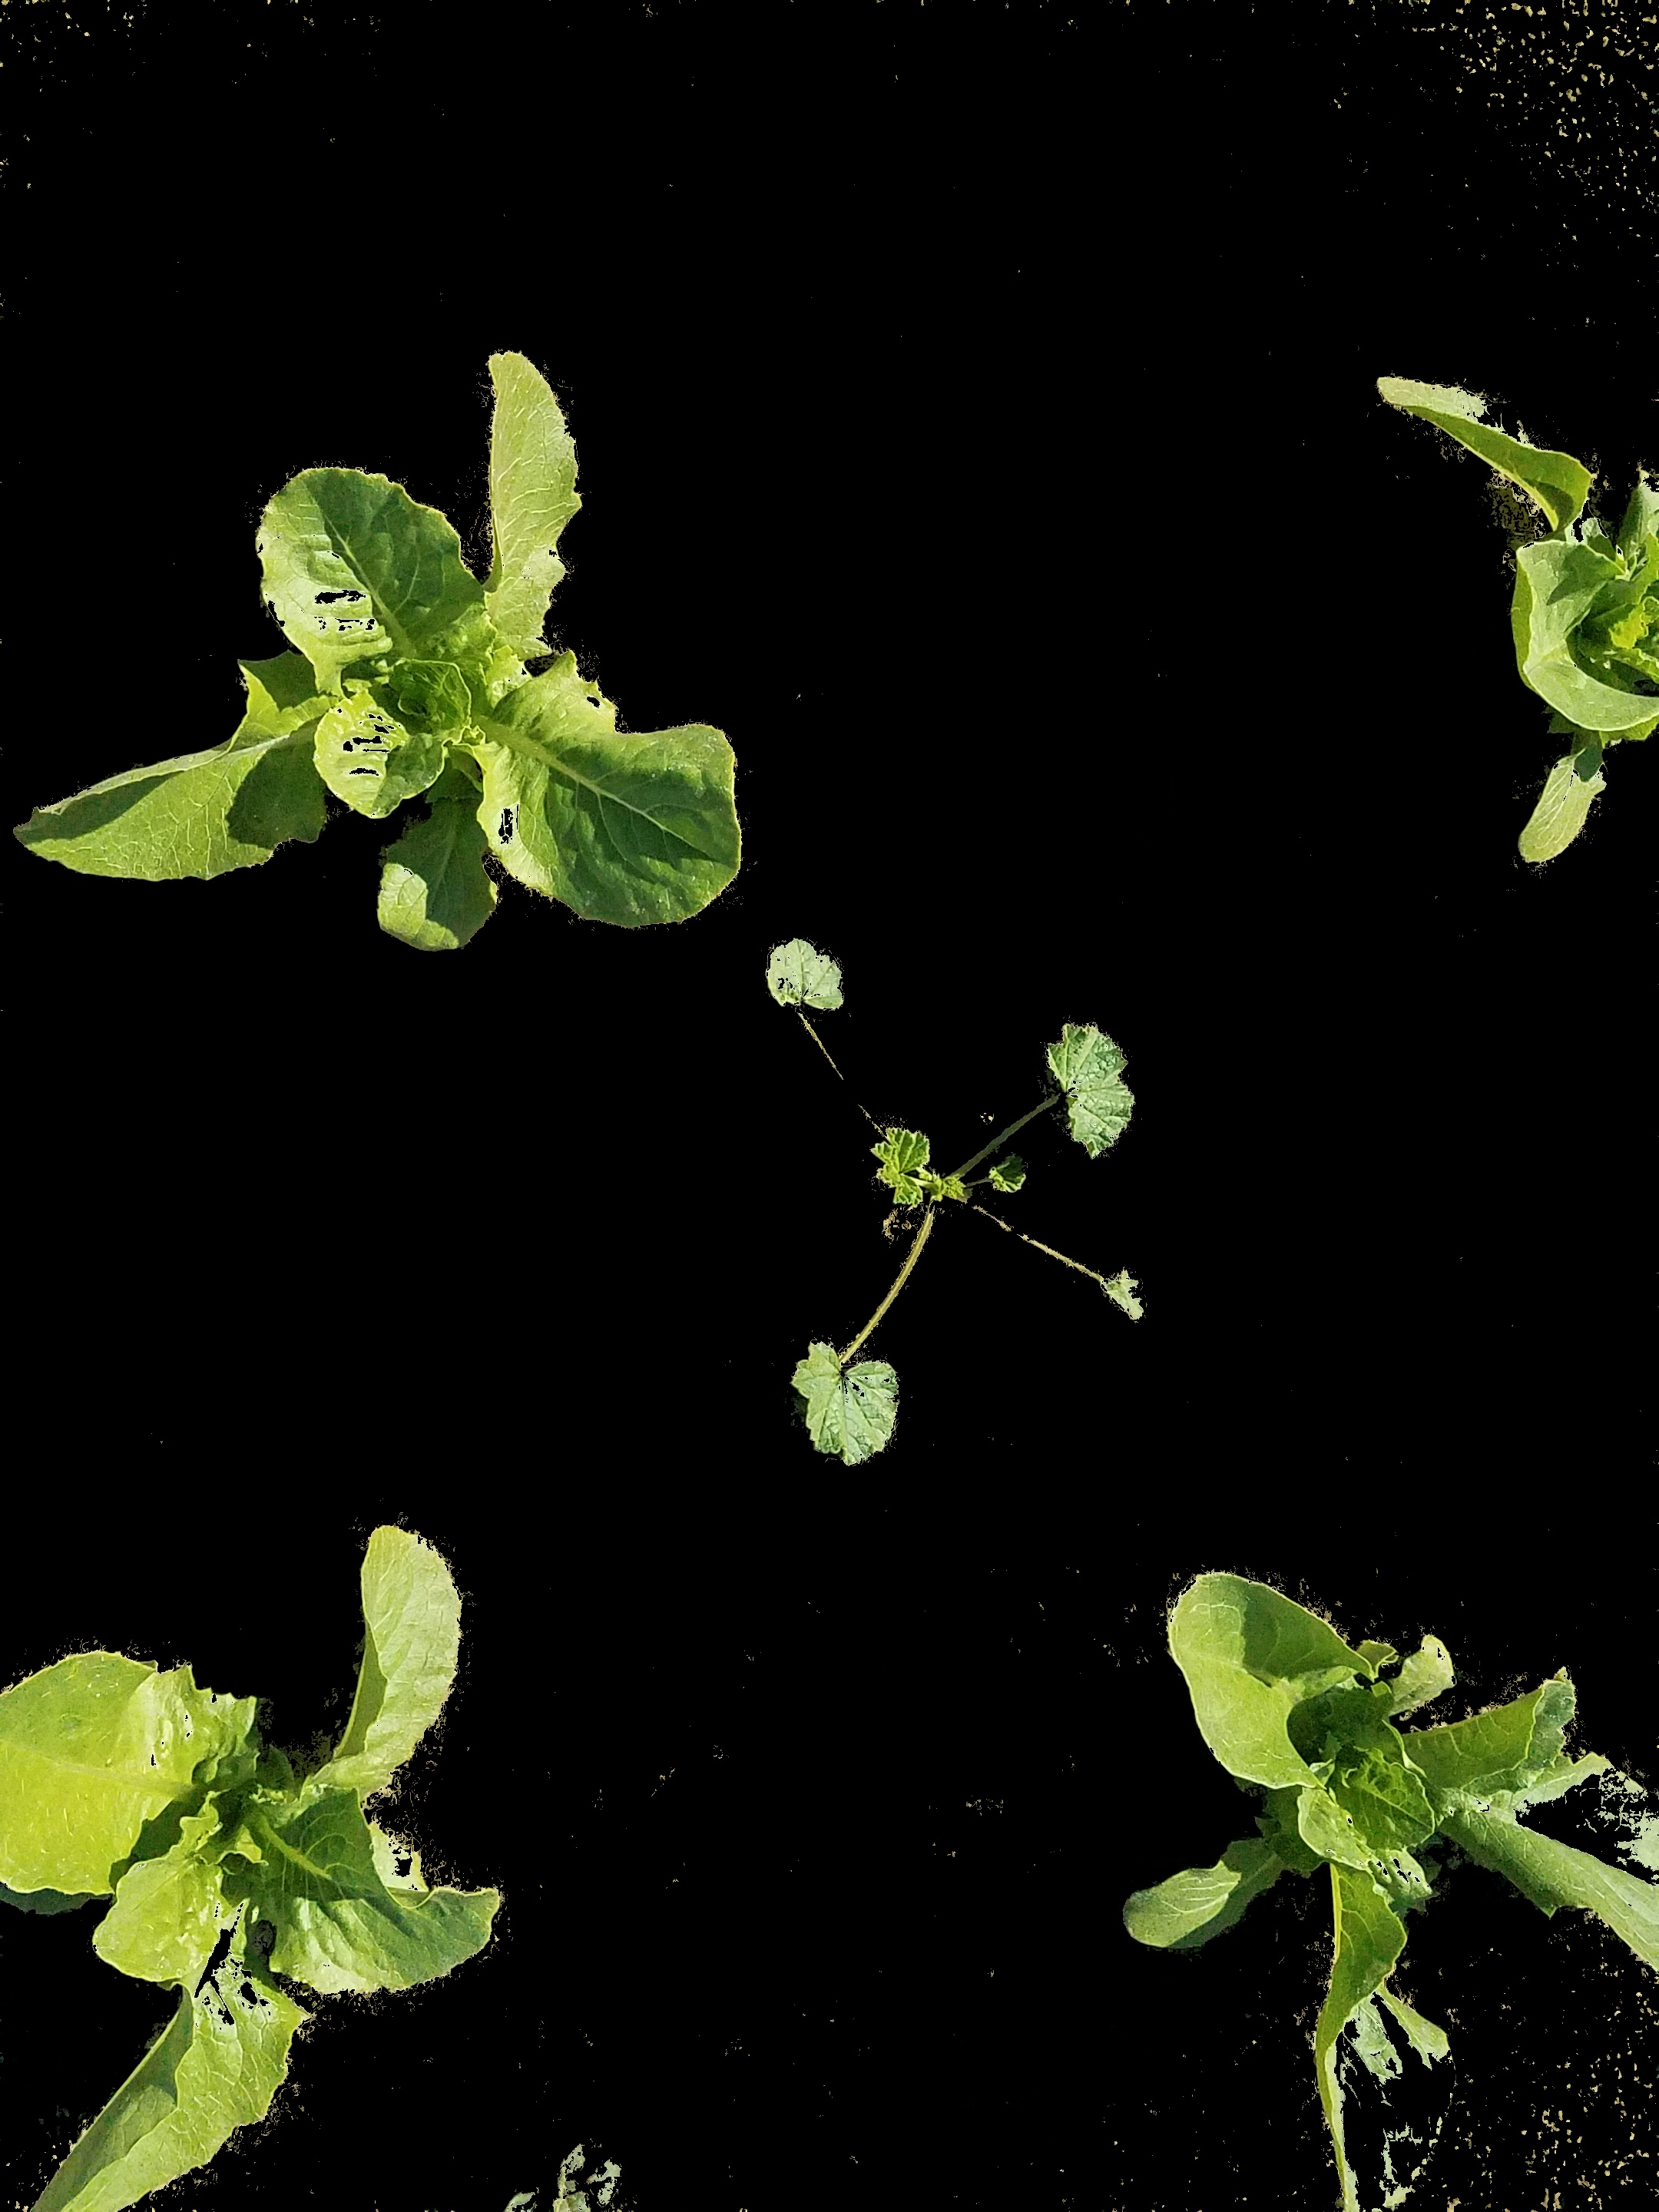
\includegraphics[height=0.10\textheight]{figures/20201117_112624-ExG.jpg} \label{fig:exg}} &
\subfloat[EXR]{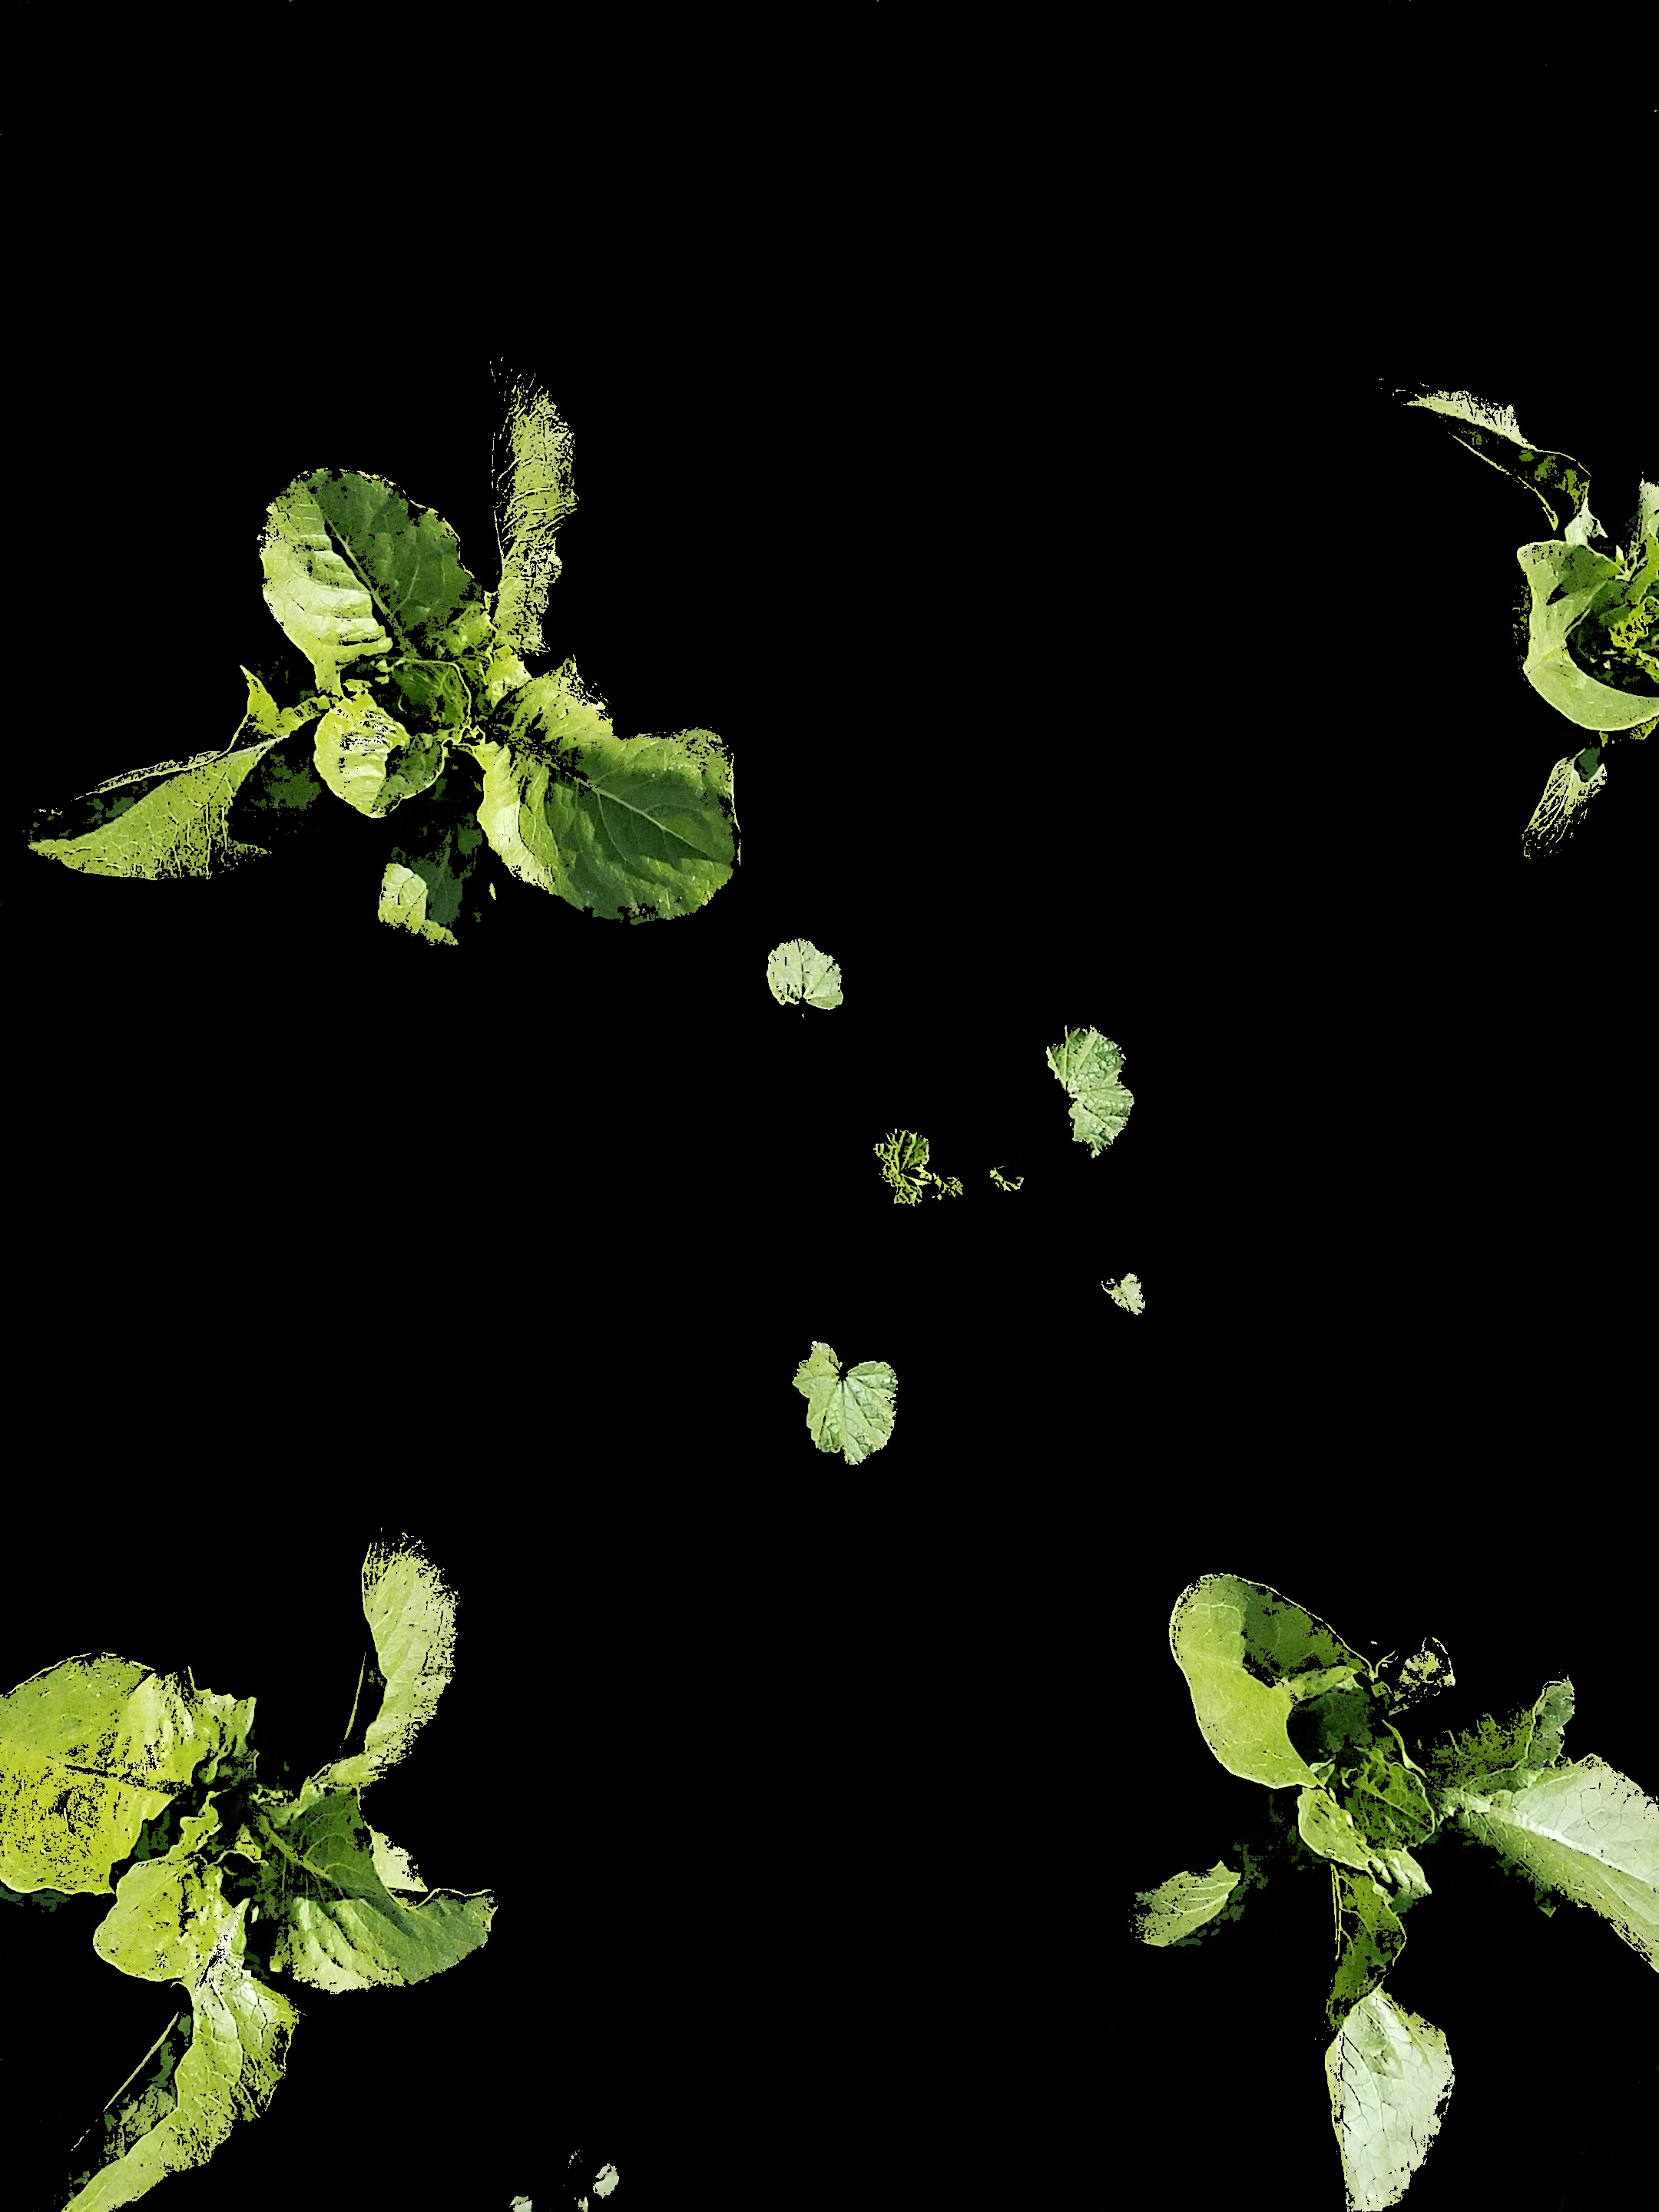
\includegraphics[height=0.10\textheight]{figures/20201117_112624-ExR.jpg} \label{fig:exr}} &
\subfloat[CIVE]{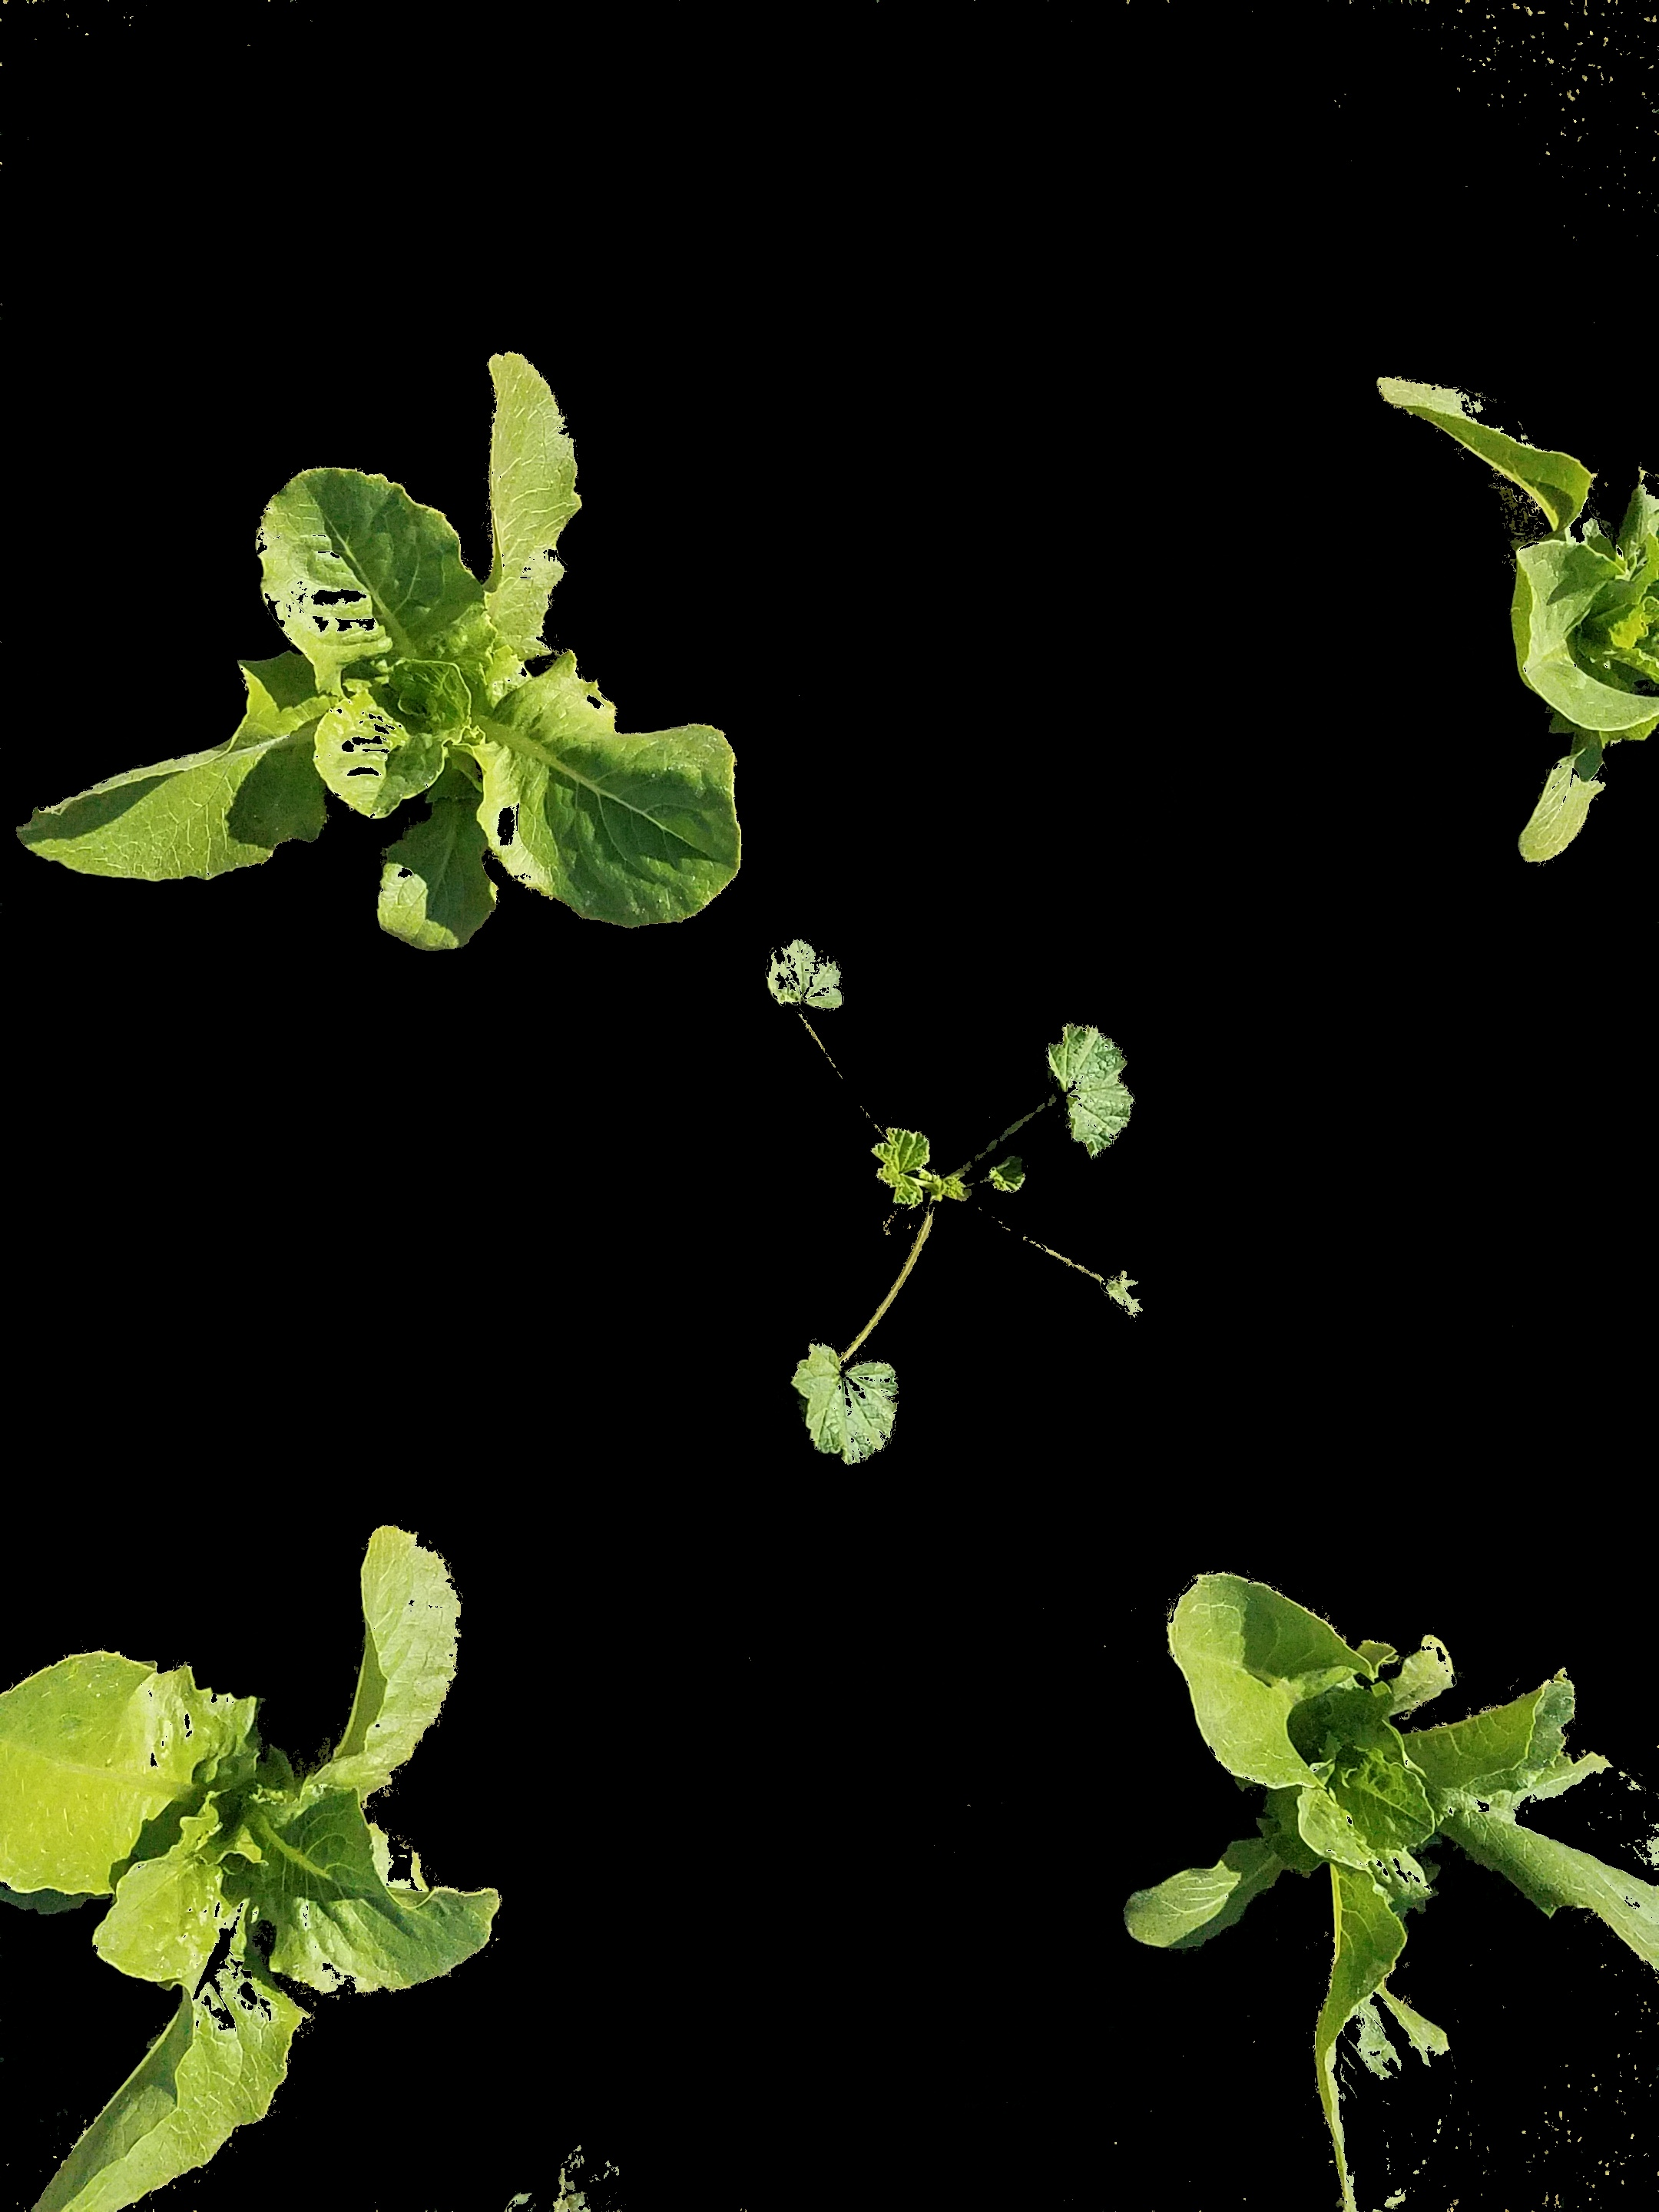
\includegraphics[height=0.10\textheight]{figures/20201117_112624-CIVE.jpg} \label{fig:cive}} &
\subfloat[EXG-EXR]{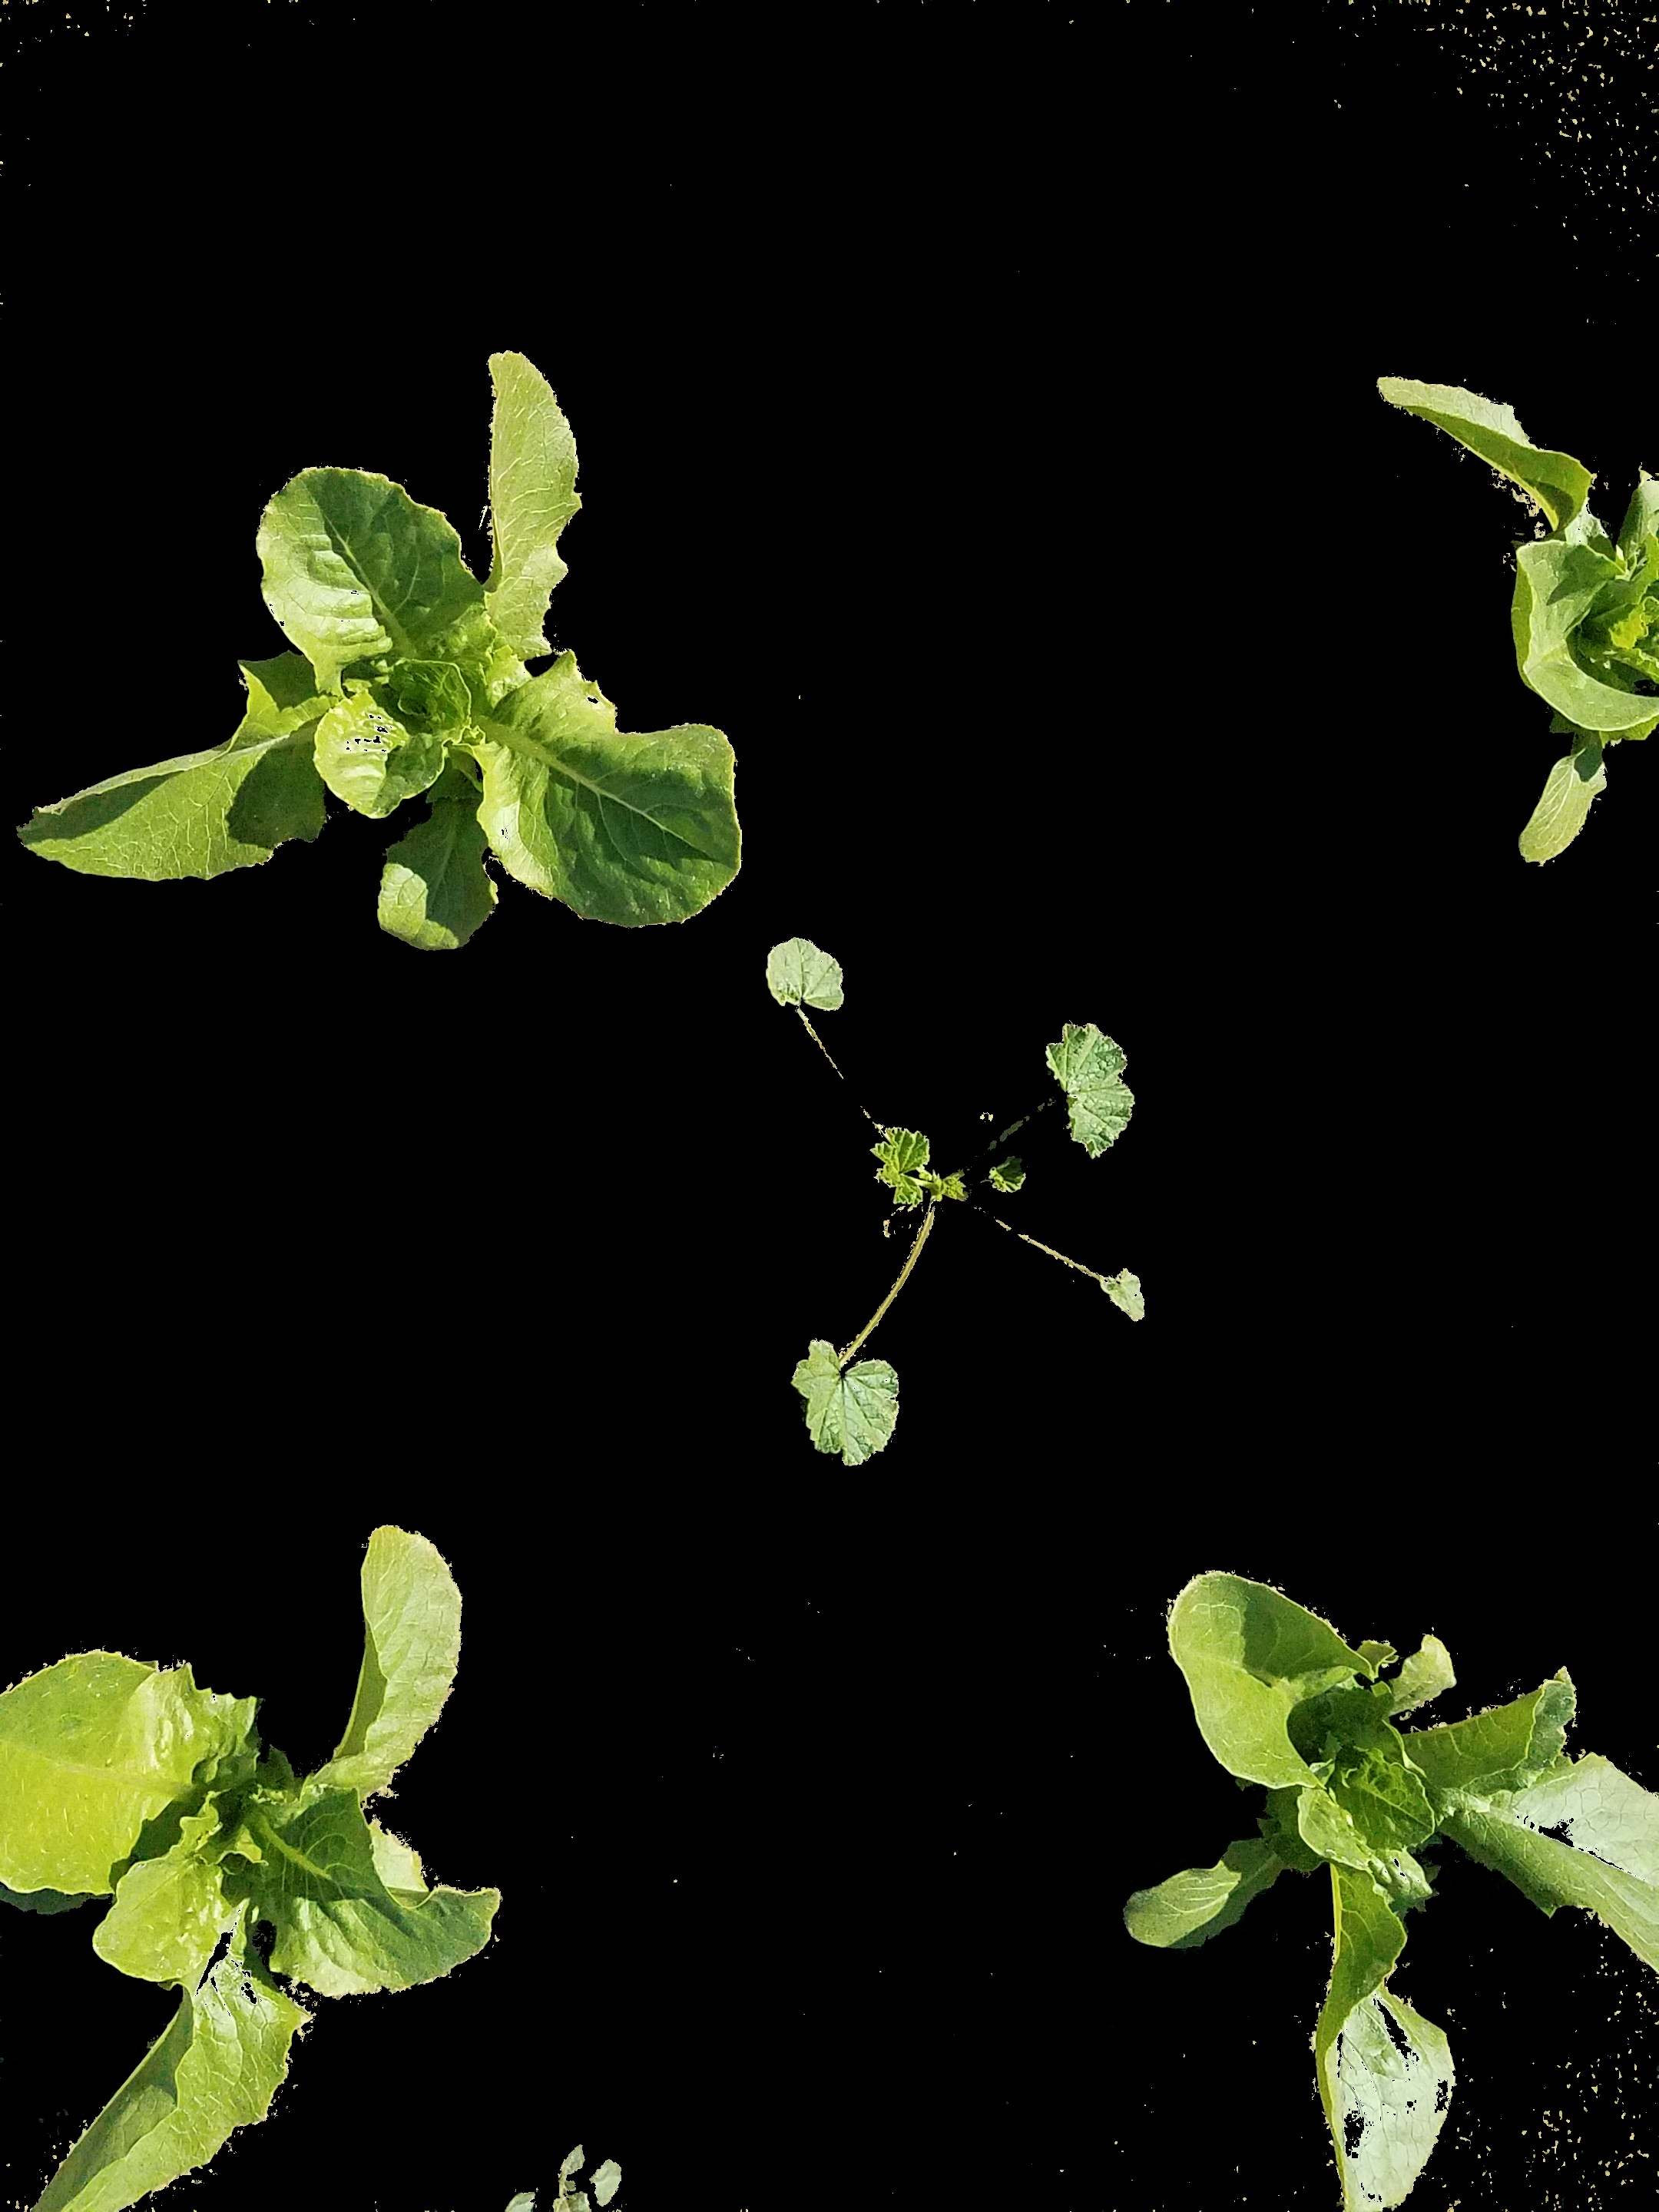
\includegraphics[height=0.10\textheight]{figures/20201117_112624-ExGR.jpg} \label{fig:exgexr}} &
\subfloat[NGRDI]{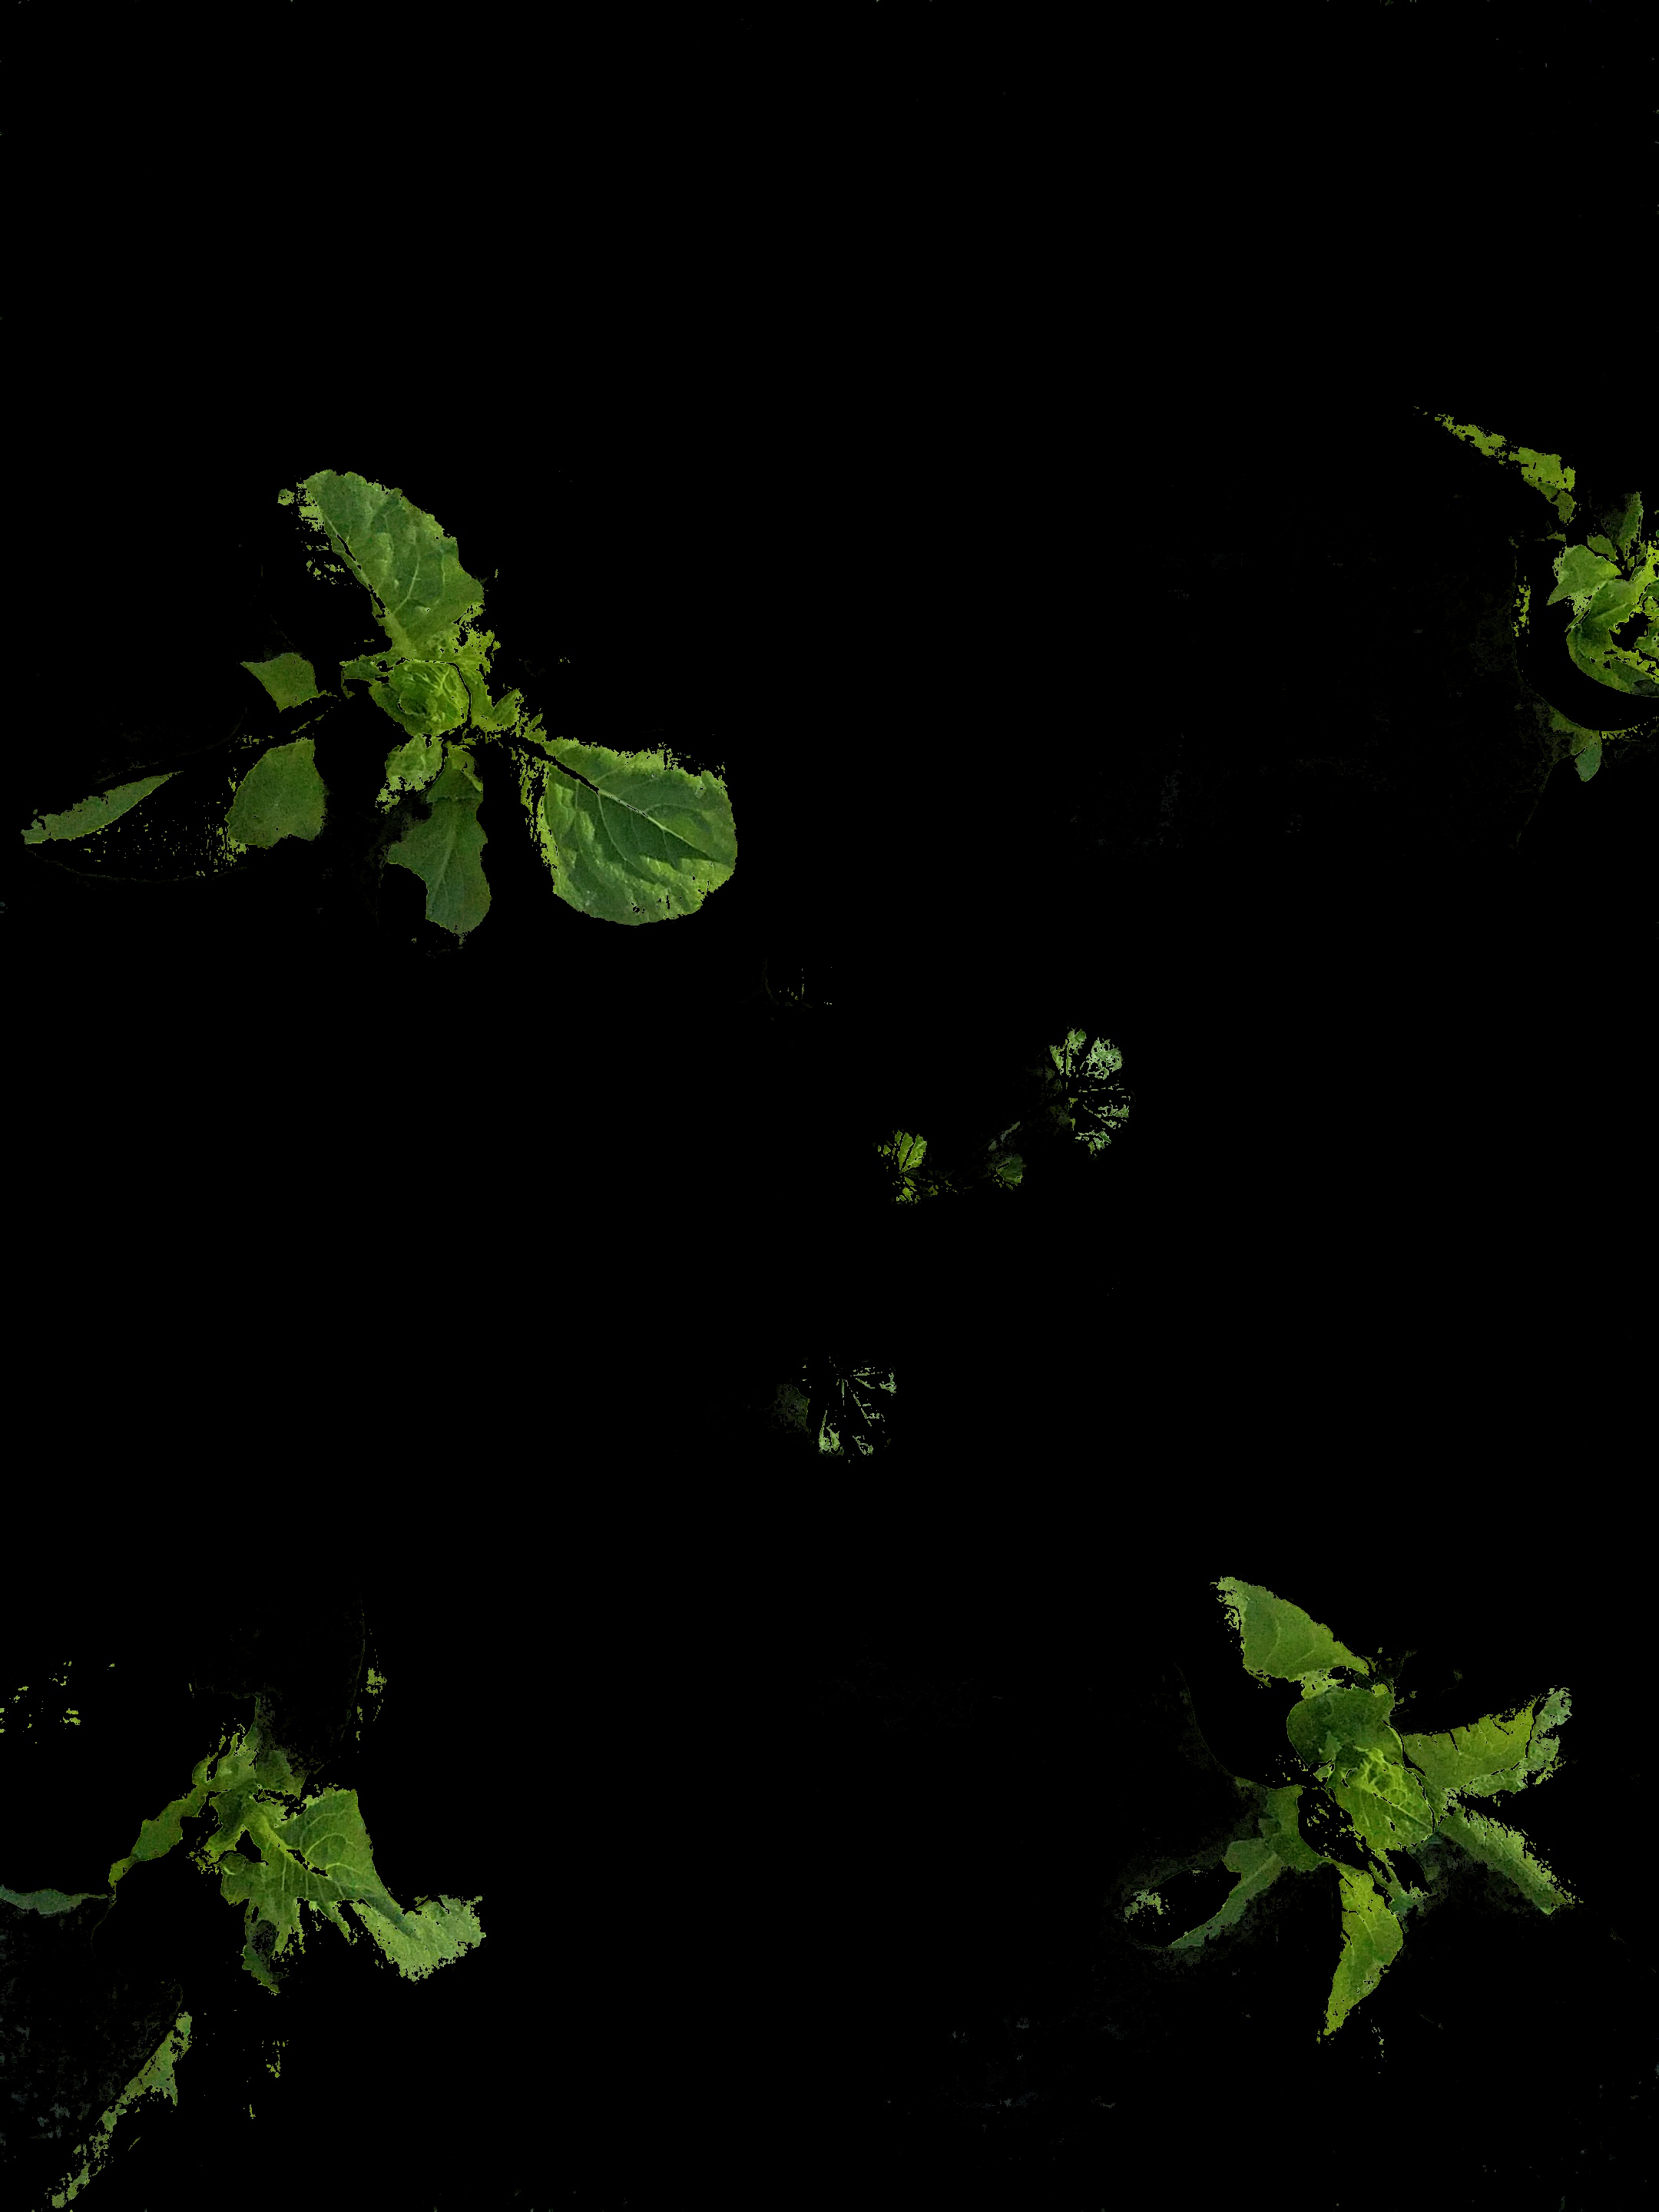
\includegraphics[height=0.10\textheight]{figures/20201117_112624-NGRDI.jpg} \label{fig:nrgdi}} \\
\subfloat[Com1]{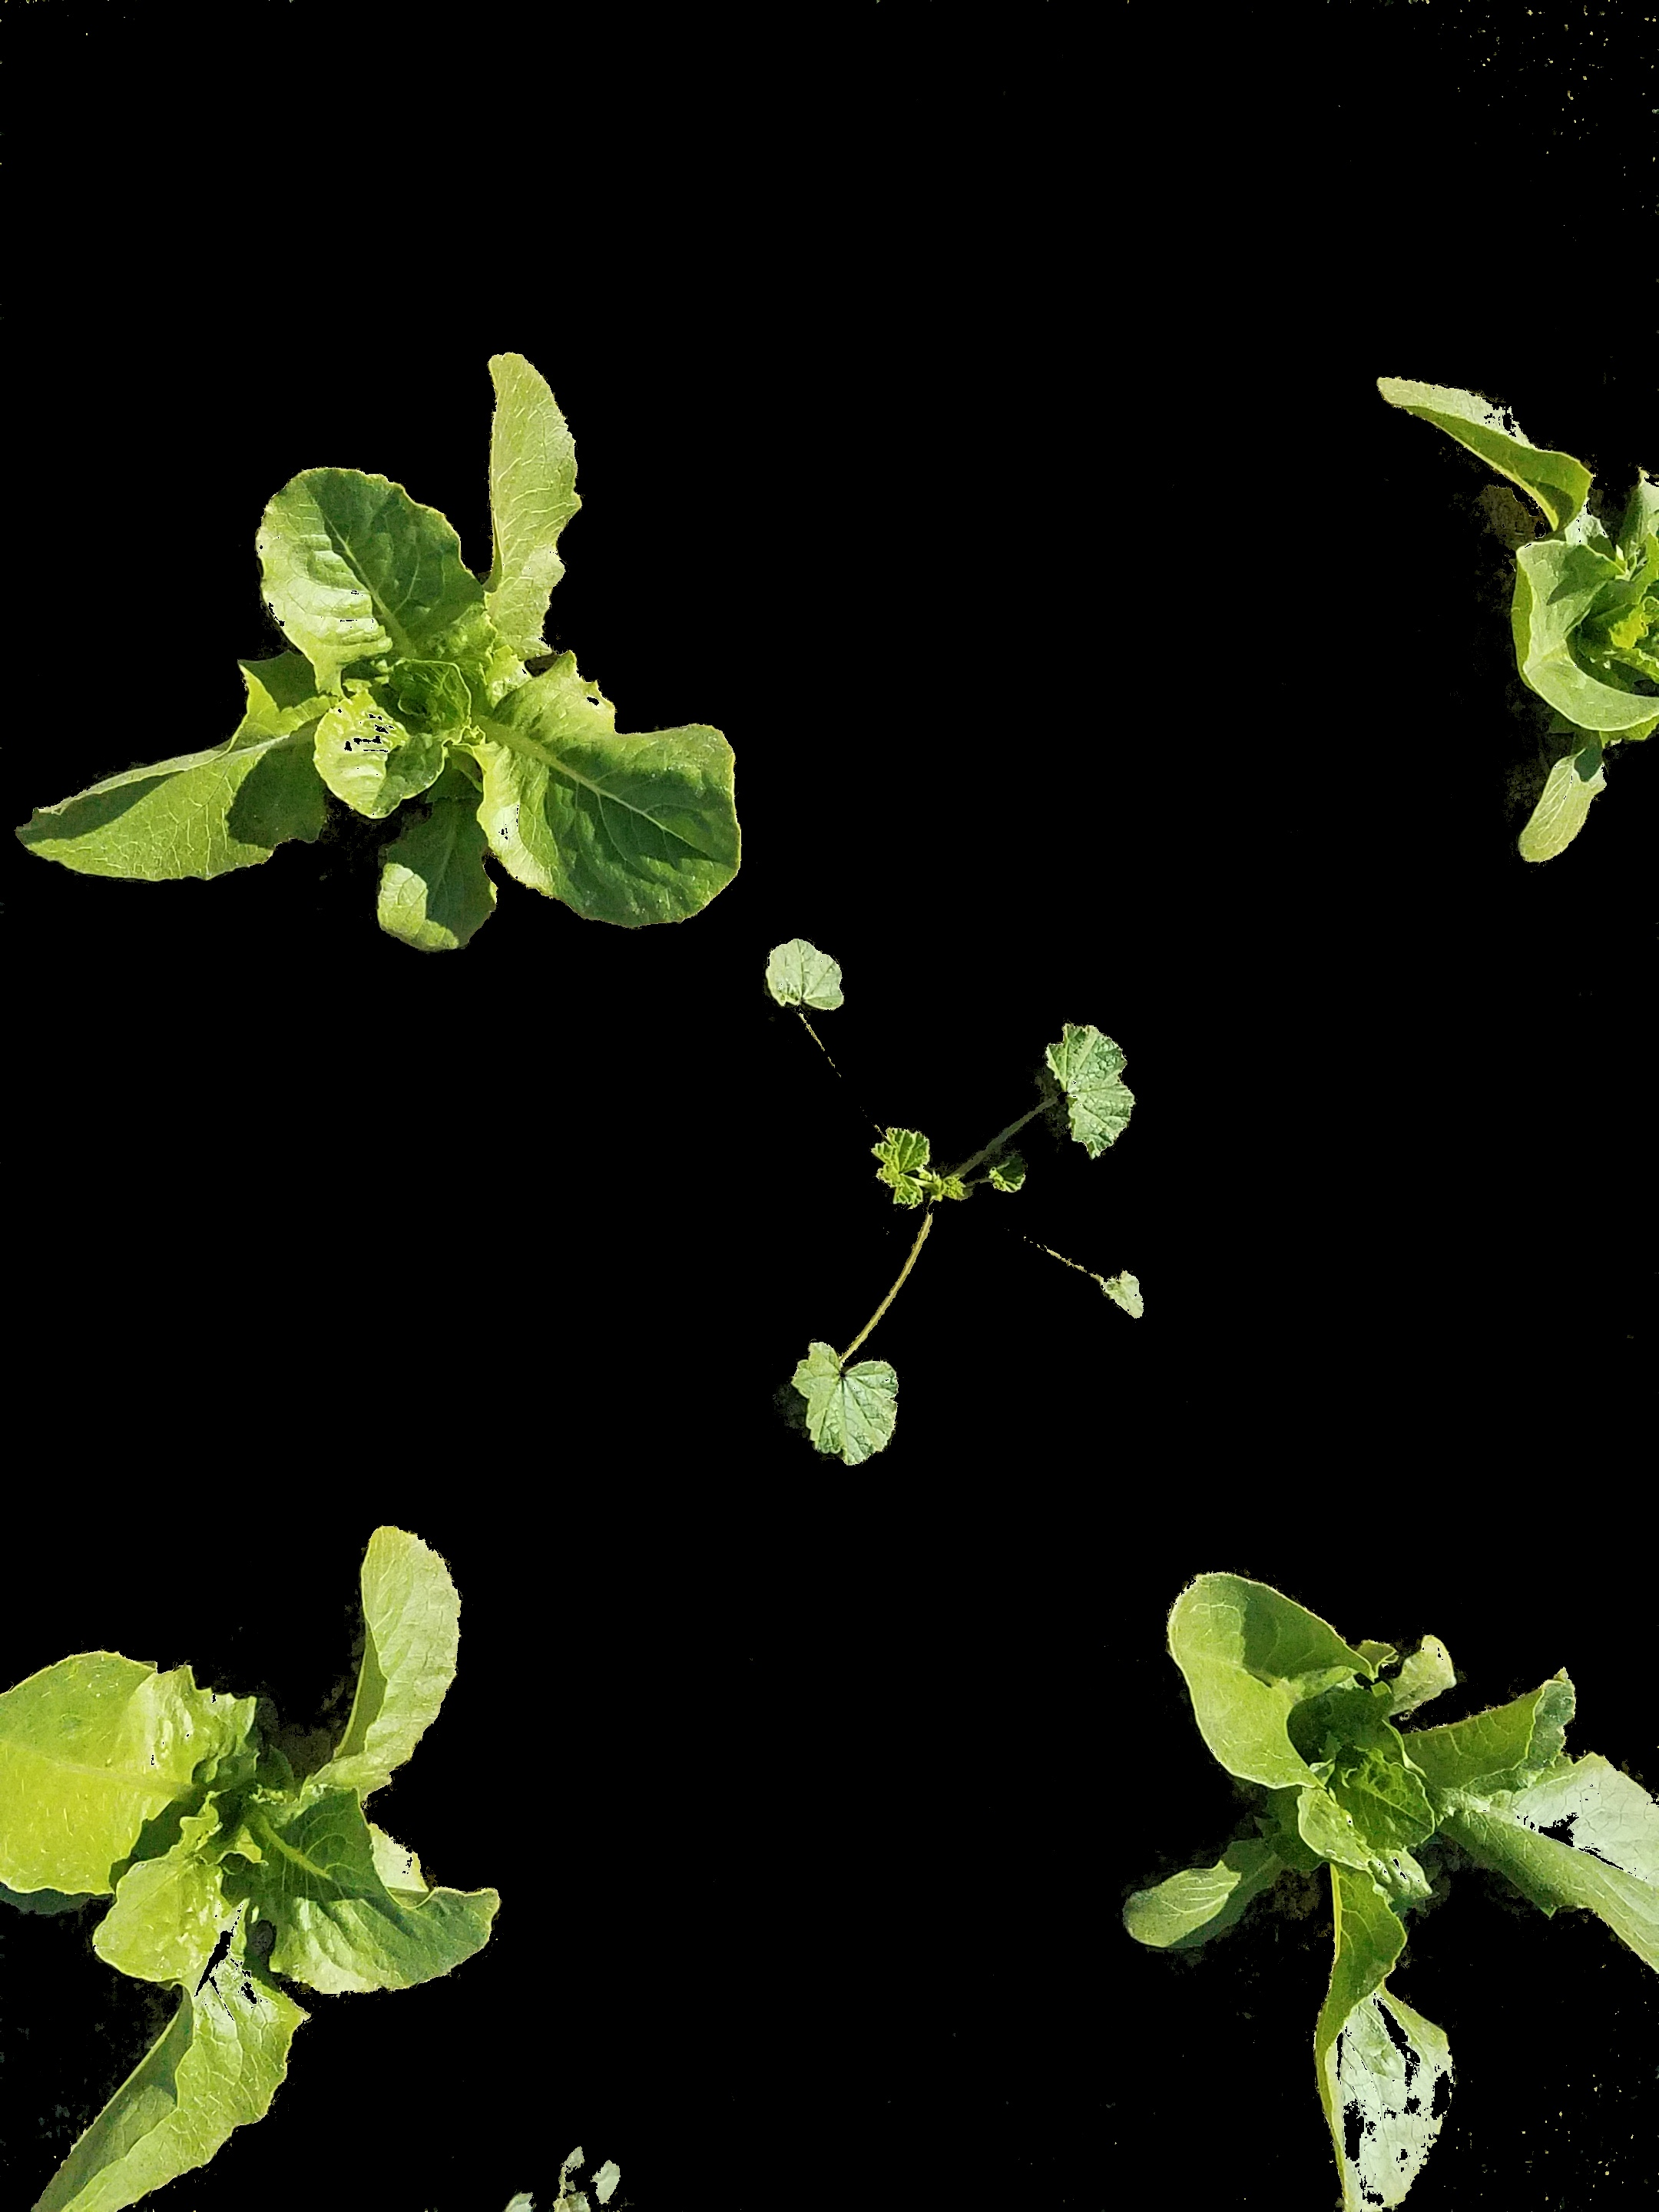
\includegraphics[height=0.10\textheight]{figures/20201117_112624-COM1.jpg} \label{fig:com1}} &
\subfloat[Com2]{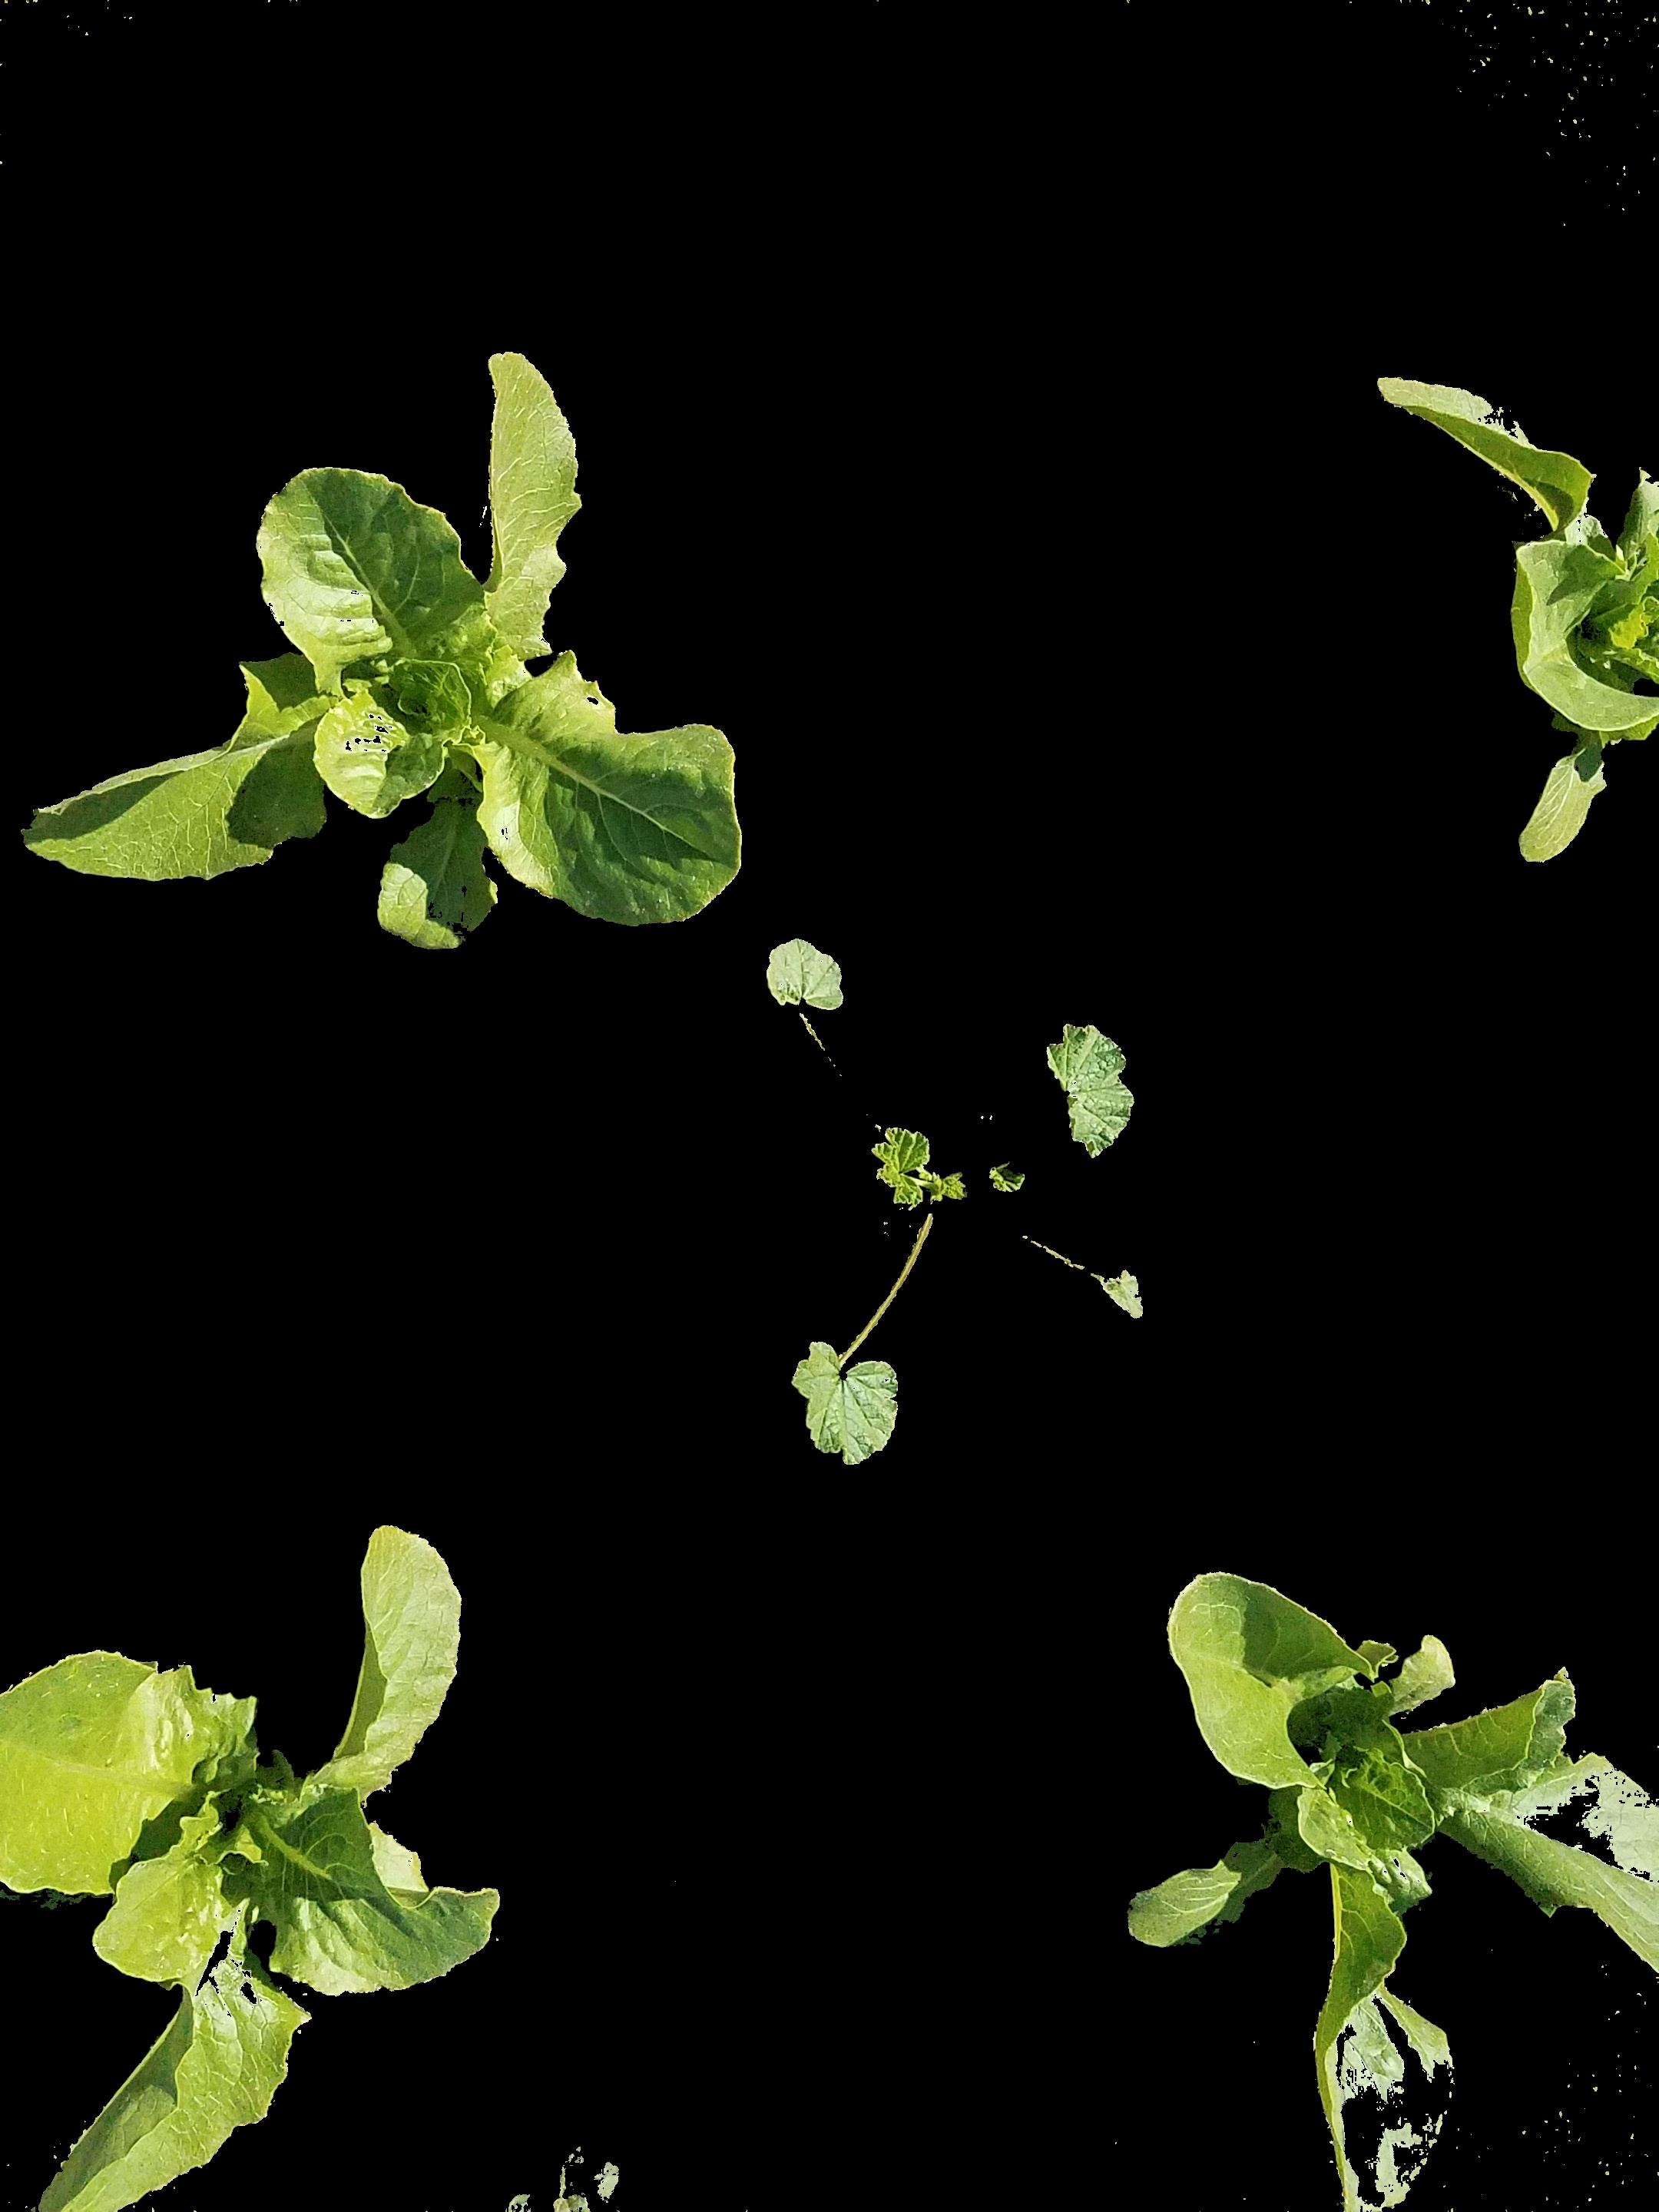
\includegraphics[height=0.10\textheight]{figures/20201117_112624-COM2.jpg} \label{fig:com2}}&
\subfloat[MEXG]{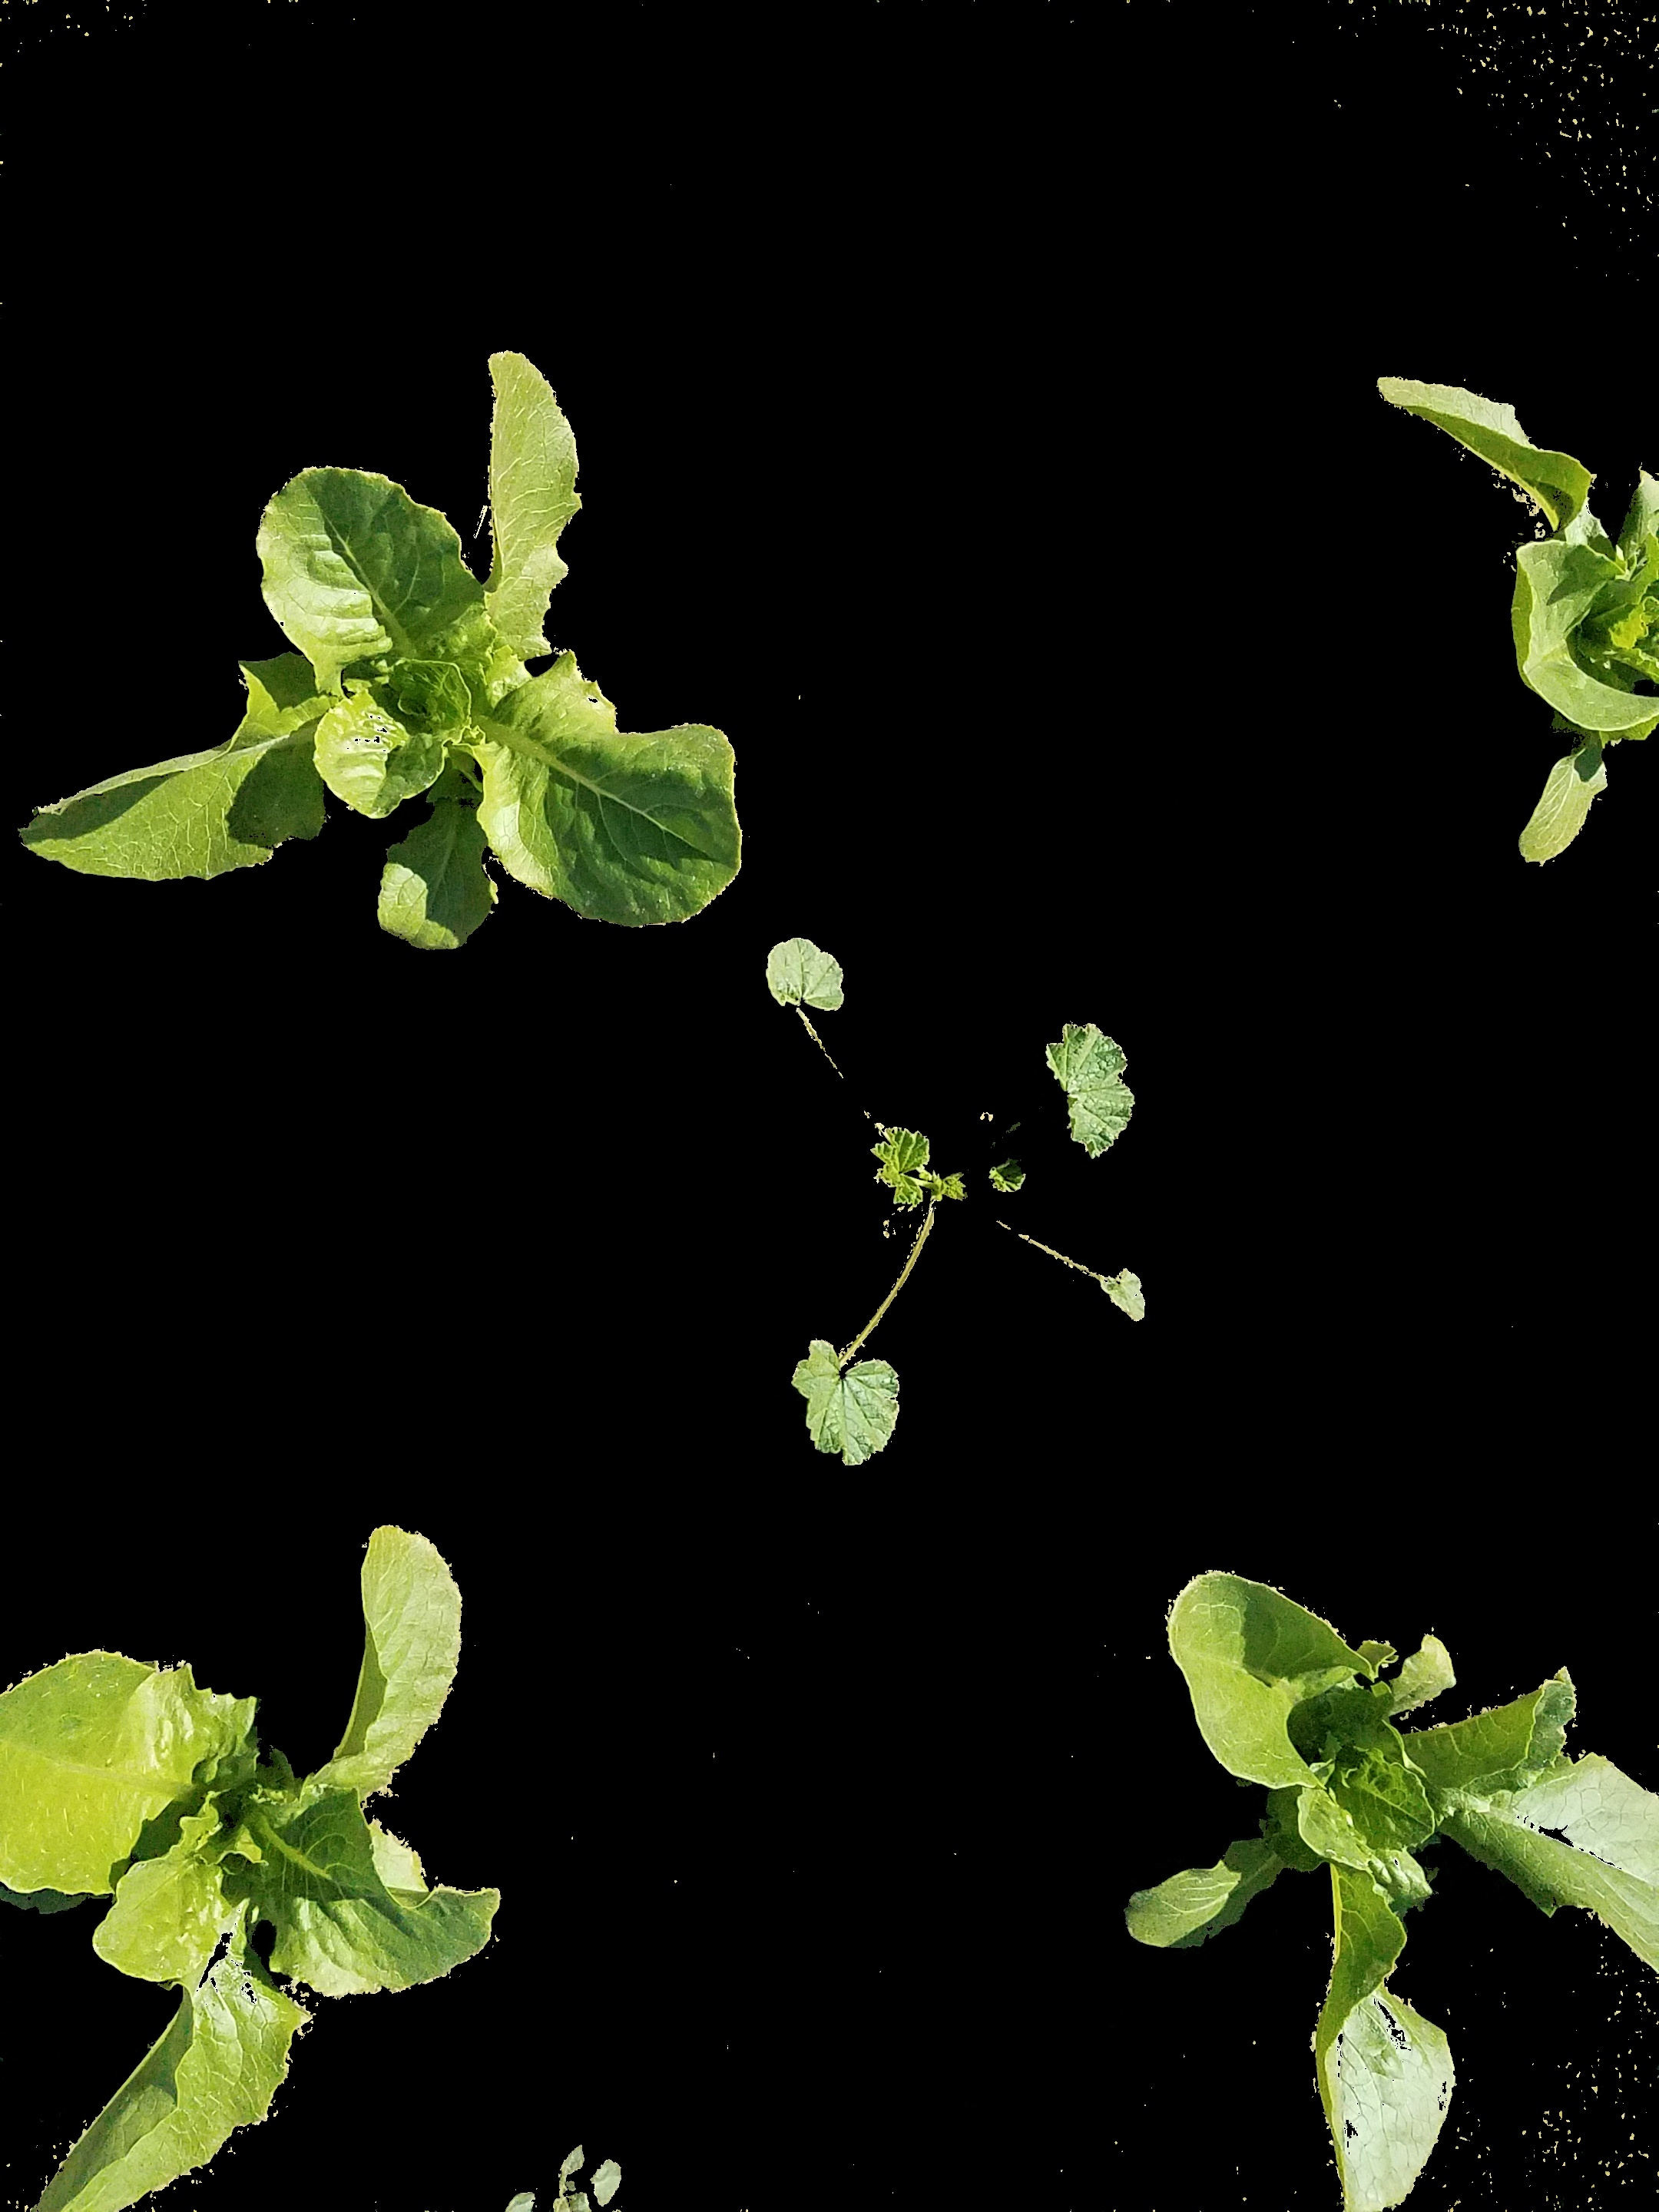
\includegraphics[height=0.10\textheight]{figures/20201117_112624-MexG.jpg} \label{fig:mexg}} &
\subfloat[TGI]{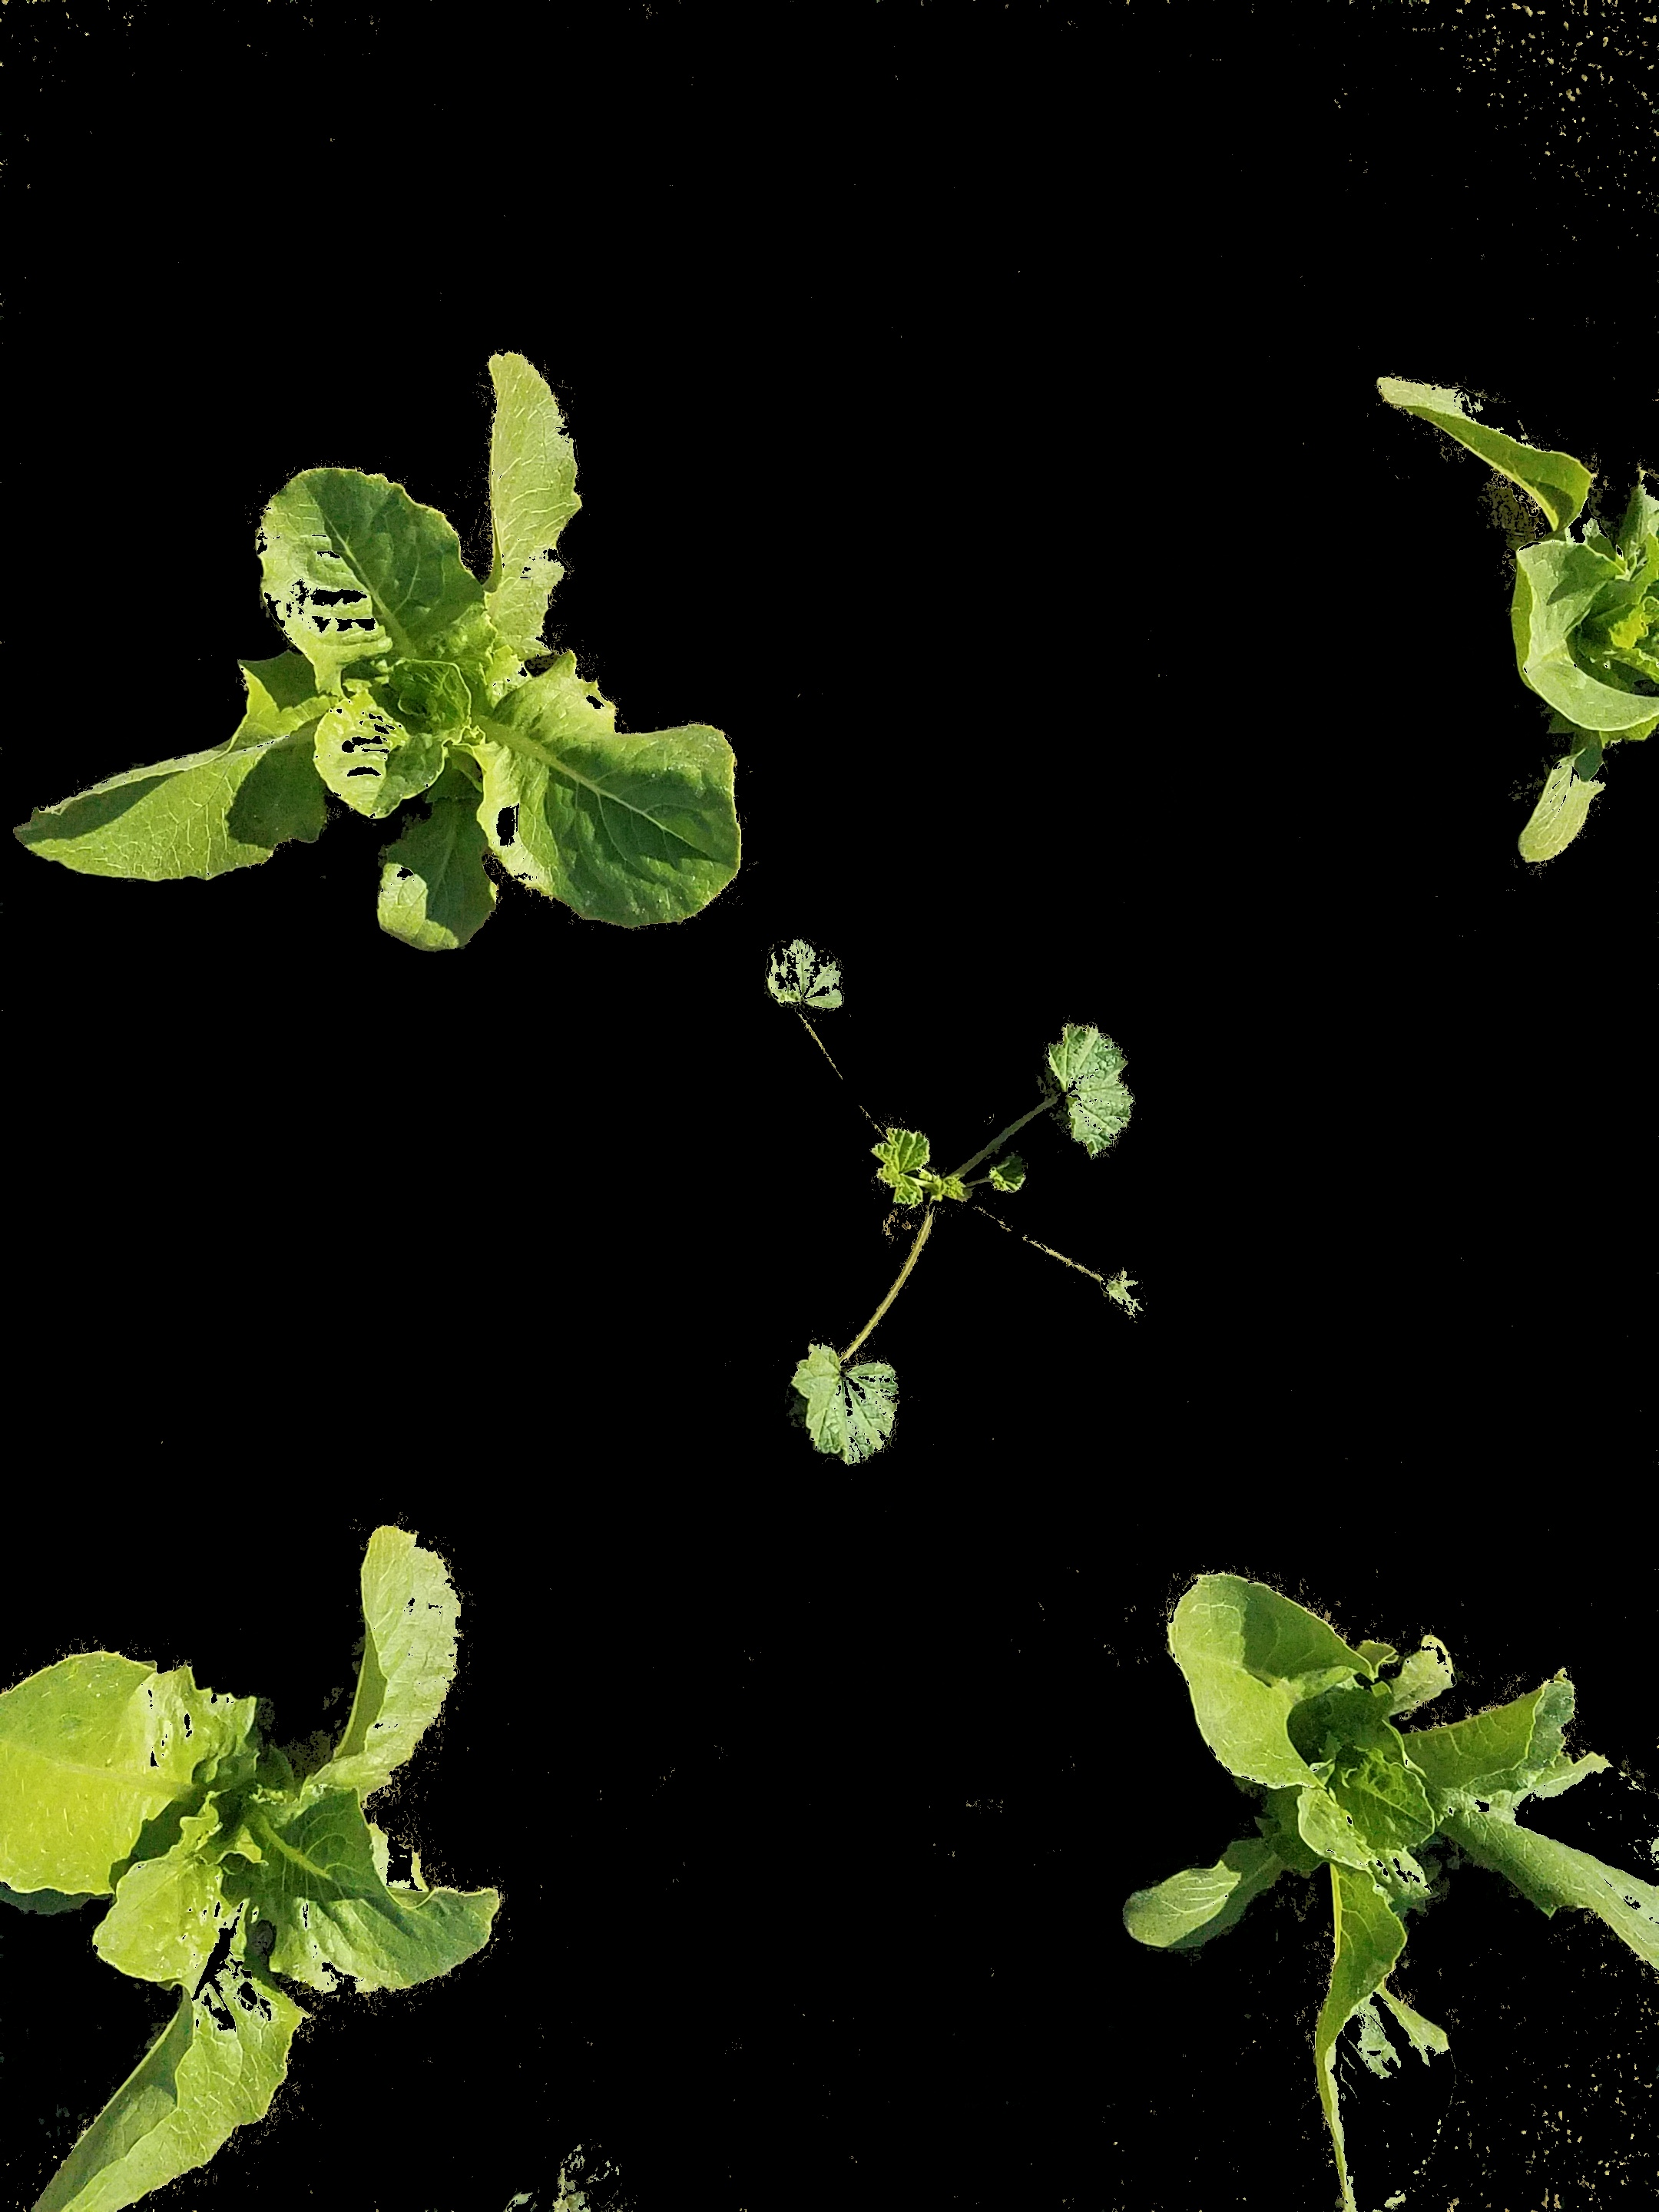
\includegraphics[height=0.10\textheight]{figures/20201117_112624-TGI.jpg} \label{fig:tgi}} &
\subfloat[VEG]{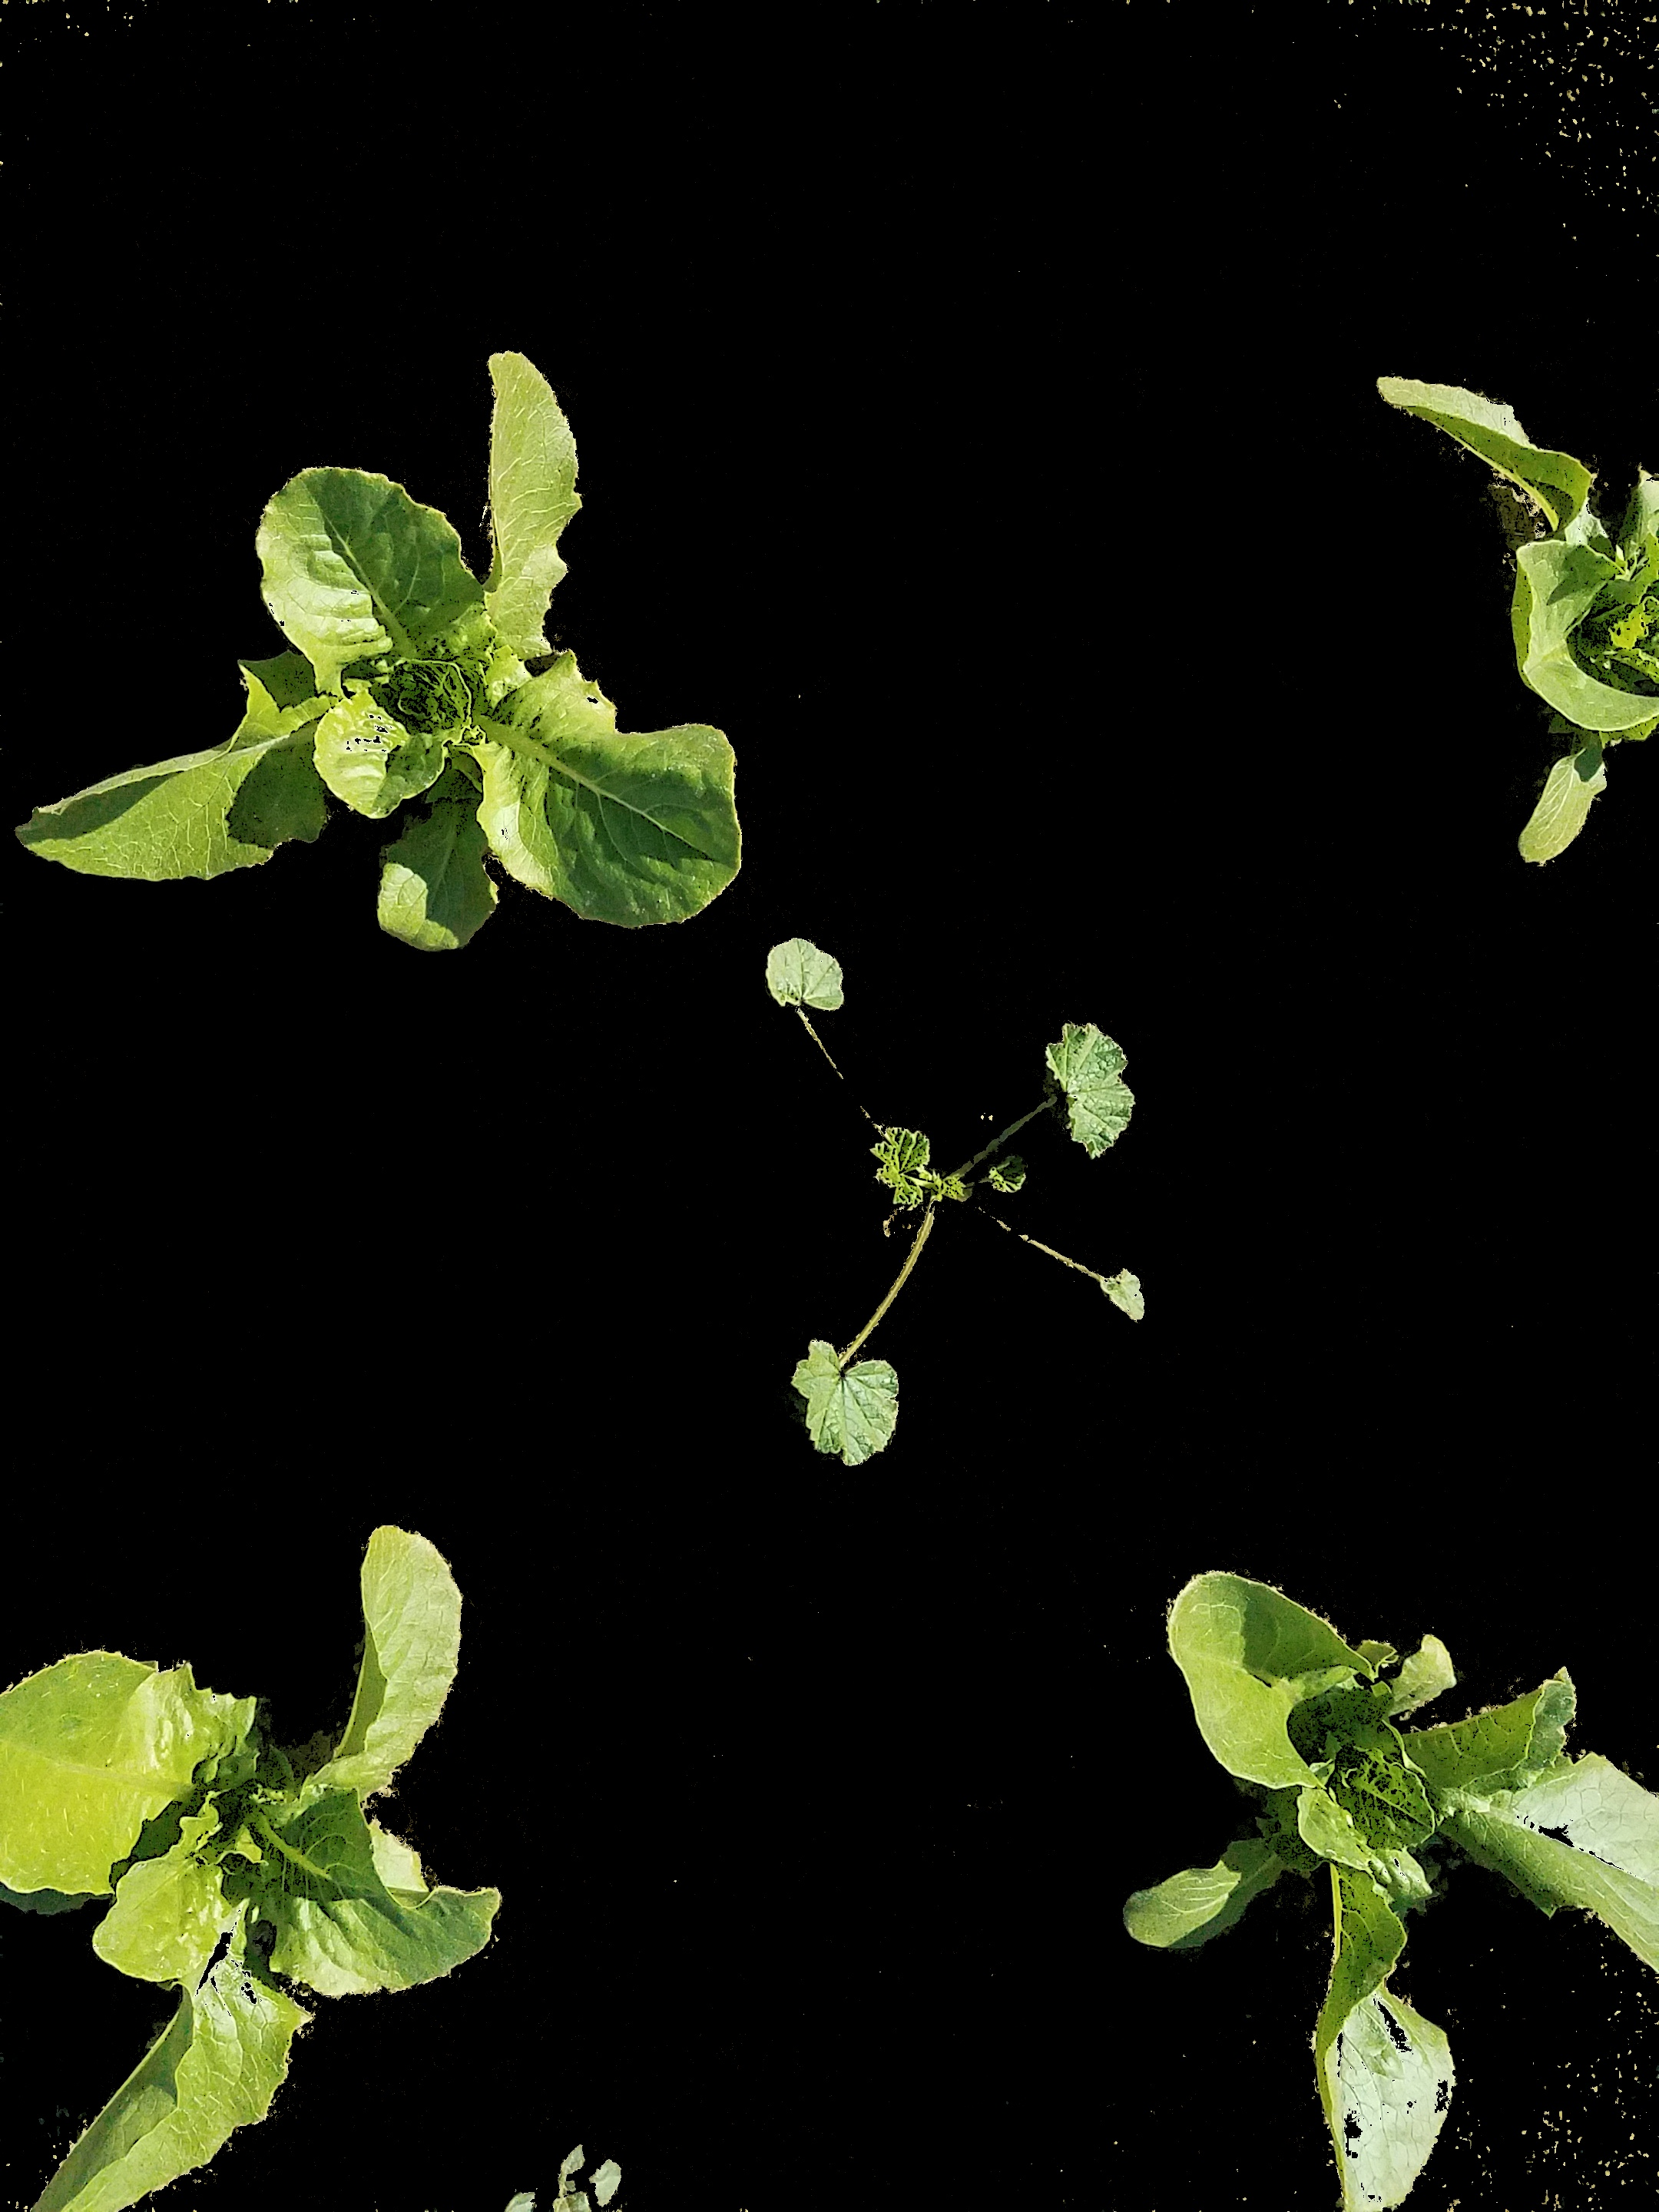
\includegraphics[height=0.10\textheight]{figures/20201117_112624-VEG.jpg} \label{fig:veg}} &
\subfloat[Original]{\includegraphics[scale=0.0215,angle=90]{figures/20201117_112624.jpg} \label{fig:original}} \\

\end{tabular}
\caption[Results of various visible-light image segmentation techniques]{Various visible-light image segmentation techniques (See Table \ref{table:indices} for details). At first glance, many of the segmentation algorithms produce similar results, but some of the methods are not sensitive to less green portions of the plants -- slender stems. Contrast the results seen in \ref{fig:exr} and \ref{fig:mexg}, with the slender stems of the plant in the middle of the image not present in the result of the former.}
\label{figure:results}
\end{figure}

There are two sorts of mistakes encountered in segmentation, as there are only two sorts of things in the image: things that are vegetation (crop and weeds) and things that aren't (typically, the ground, but also items that are expected to appear, such as irrigation equipment). Omission of a crop leaf is apparent in Figure \ref{fig:ndi}, showing the result of using NDI.  The center plant is only partially visible in this case, and it goes without saying that what is not shown cannot be classified. Contrast that with the result shown in Figures \ref{fig:hi} and  \ref{fig:hv}, where the ground is featured. This case may be due to the shadow of the plant containing too much green as sunlight passes through the leaf. Figure \ref{fig:overlay} illustrates the effects of the index and errors -- of special note here is the error that is shown in the upper right-hand portion of Figure \ref{fig:overlay-cive}. These errors may result in the ground mistakenly identified as vegetation. Applying the NDI mask produces the errors discussed previously -- the leaf shadow is identified as vegetation. The evaluation of errors in index-based approaches is illustrated by Figure \ref{fig:segmentation-errors}.

\begin{figure}[H]
	\centering
	\subfloat[CIVE mask overlay\centering]{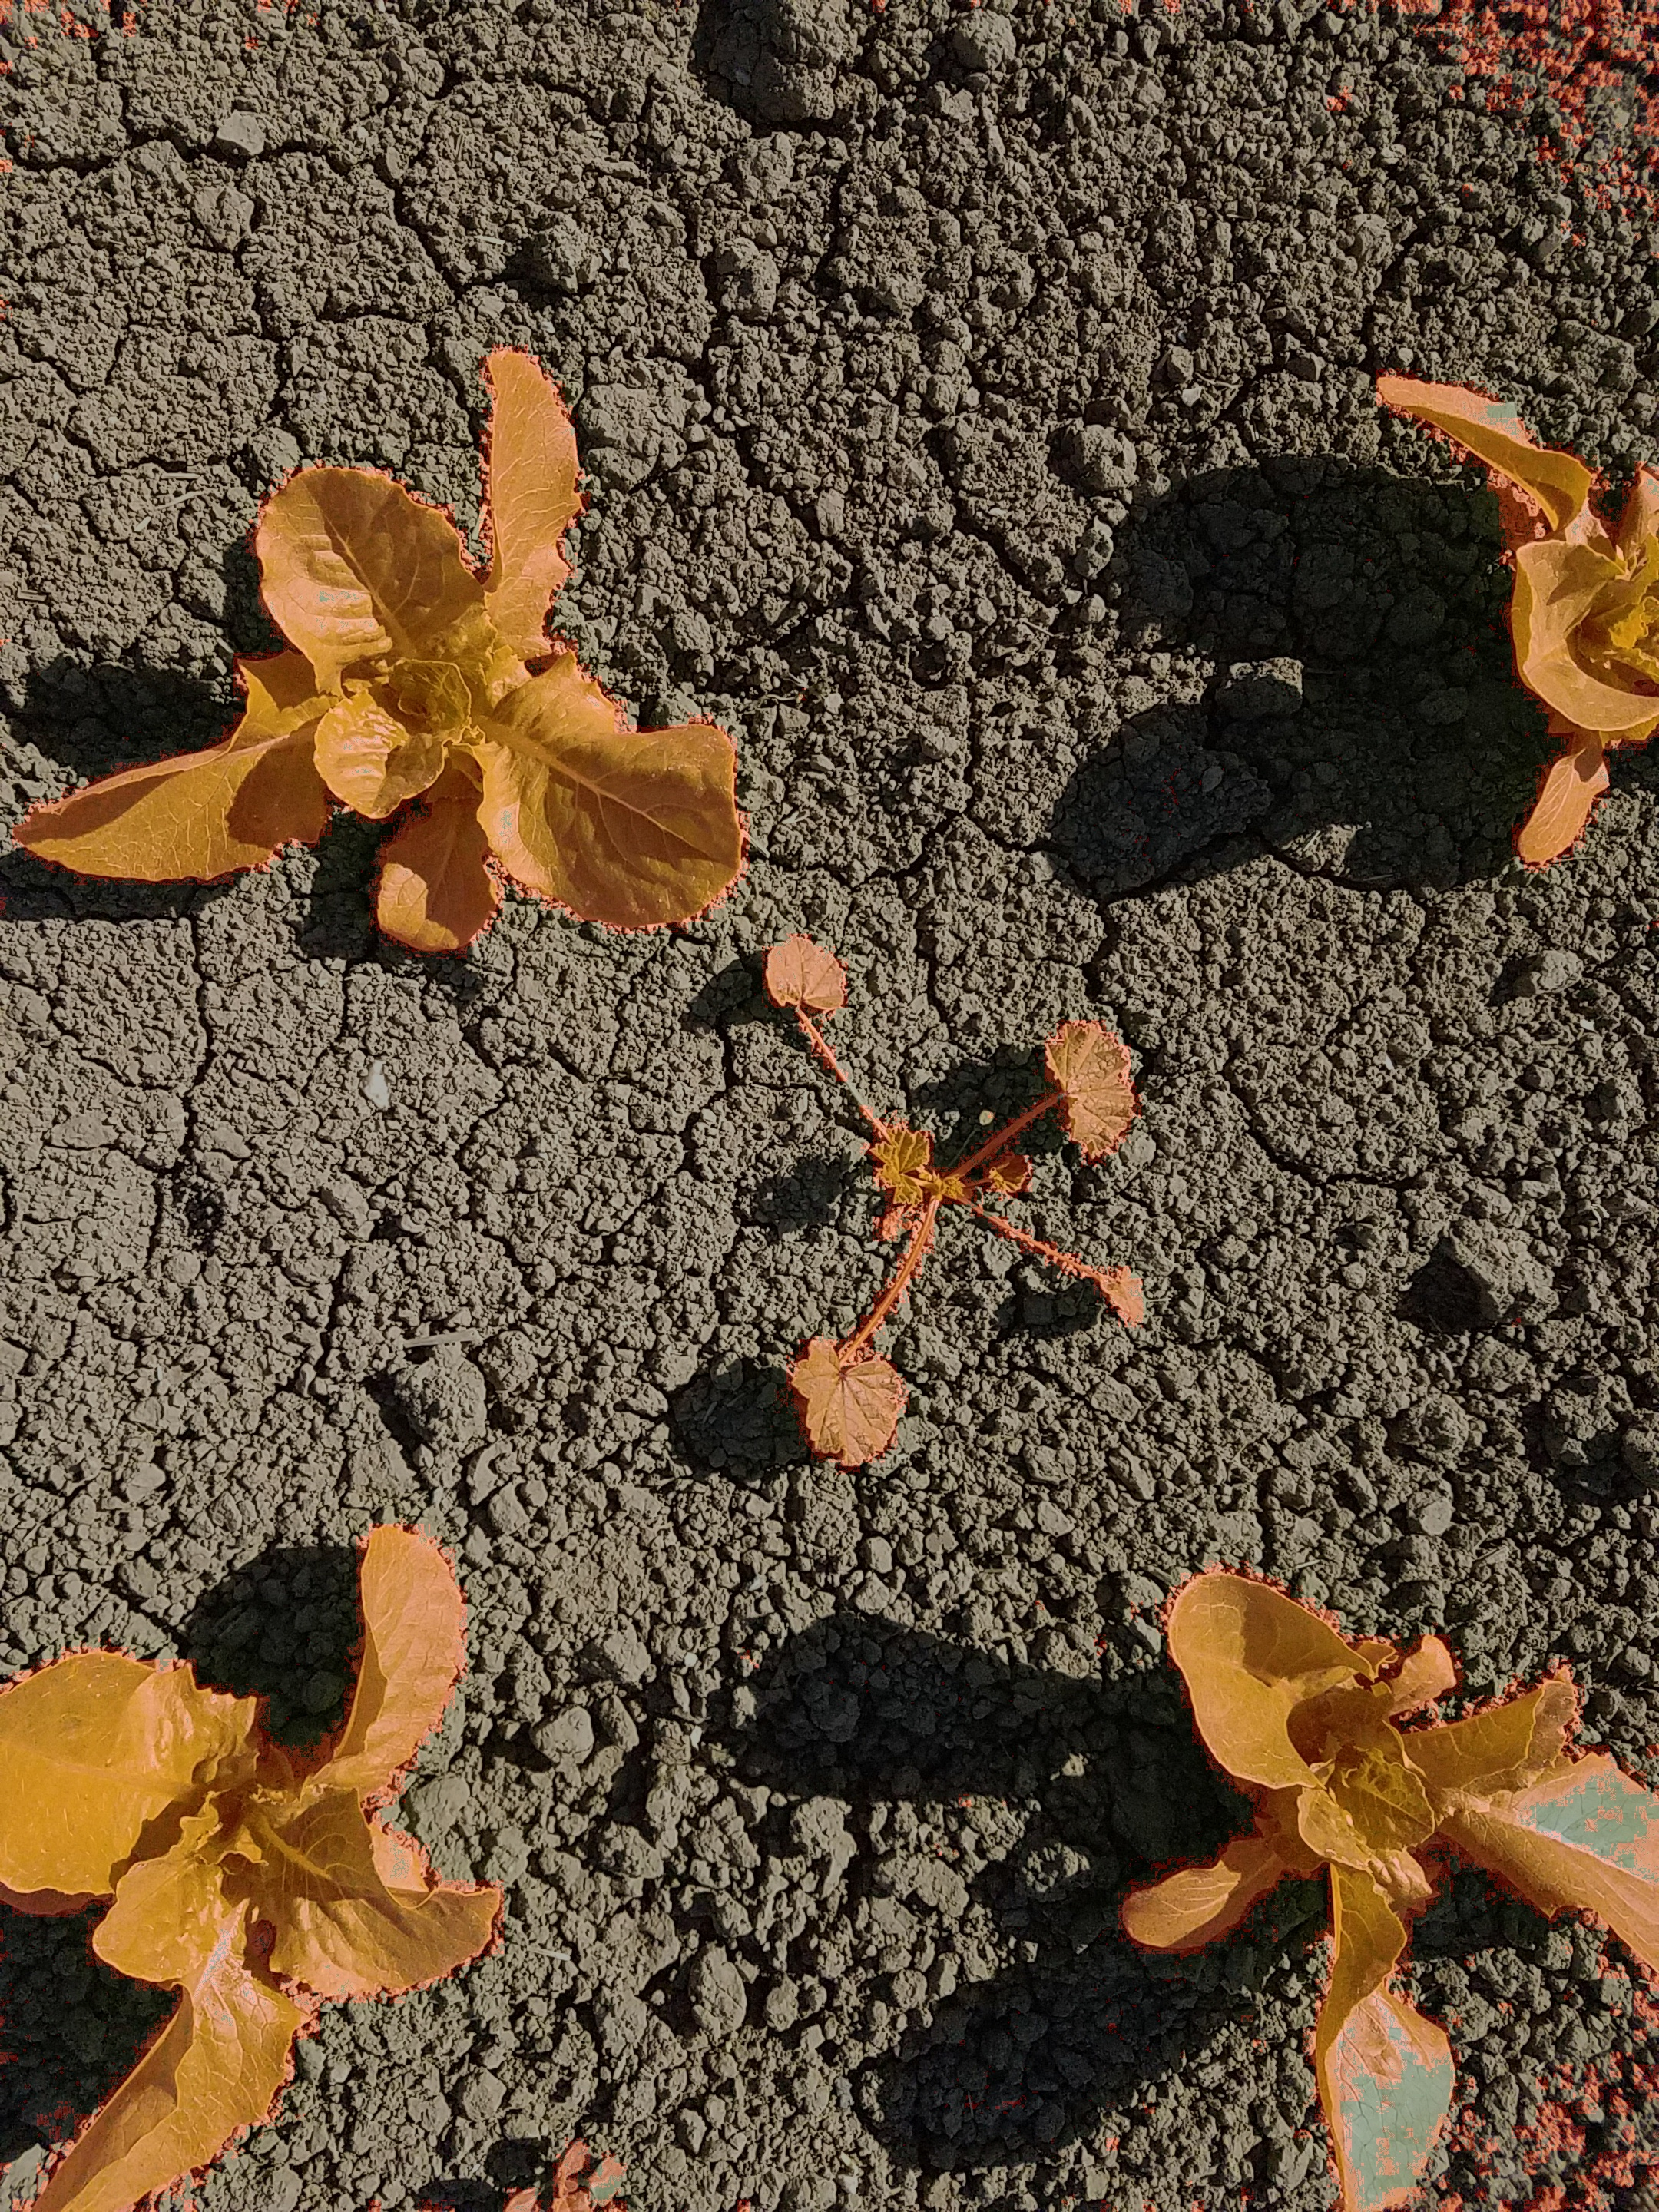
\includegraphics[width=0.45\textwidth]{figures/overlay-cive.jpg}\label{fig:overlay-cive}}
	\hfill
	\subfloat[NDI mask overlay\centering]{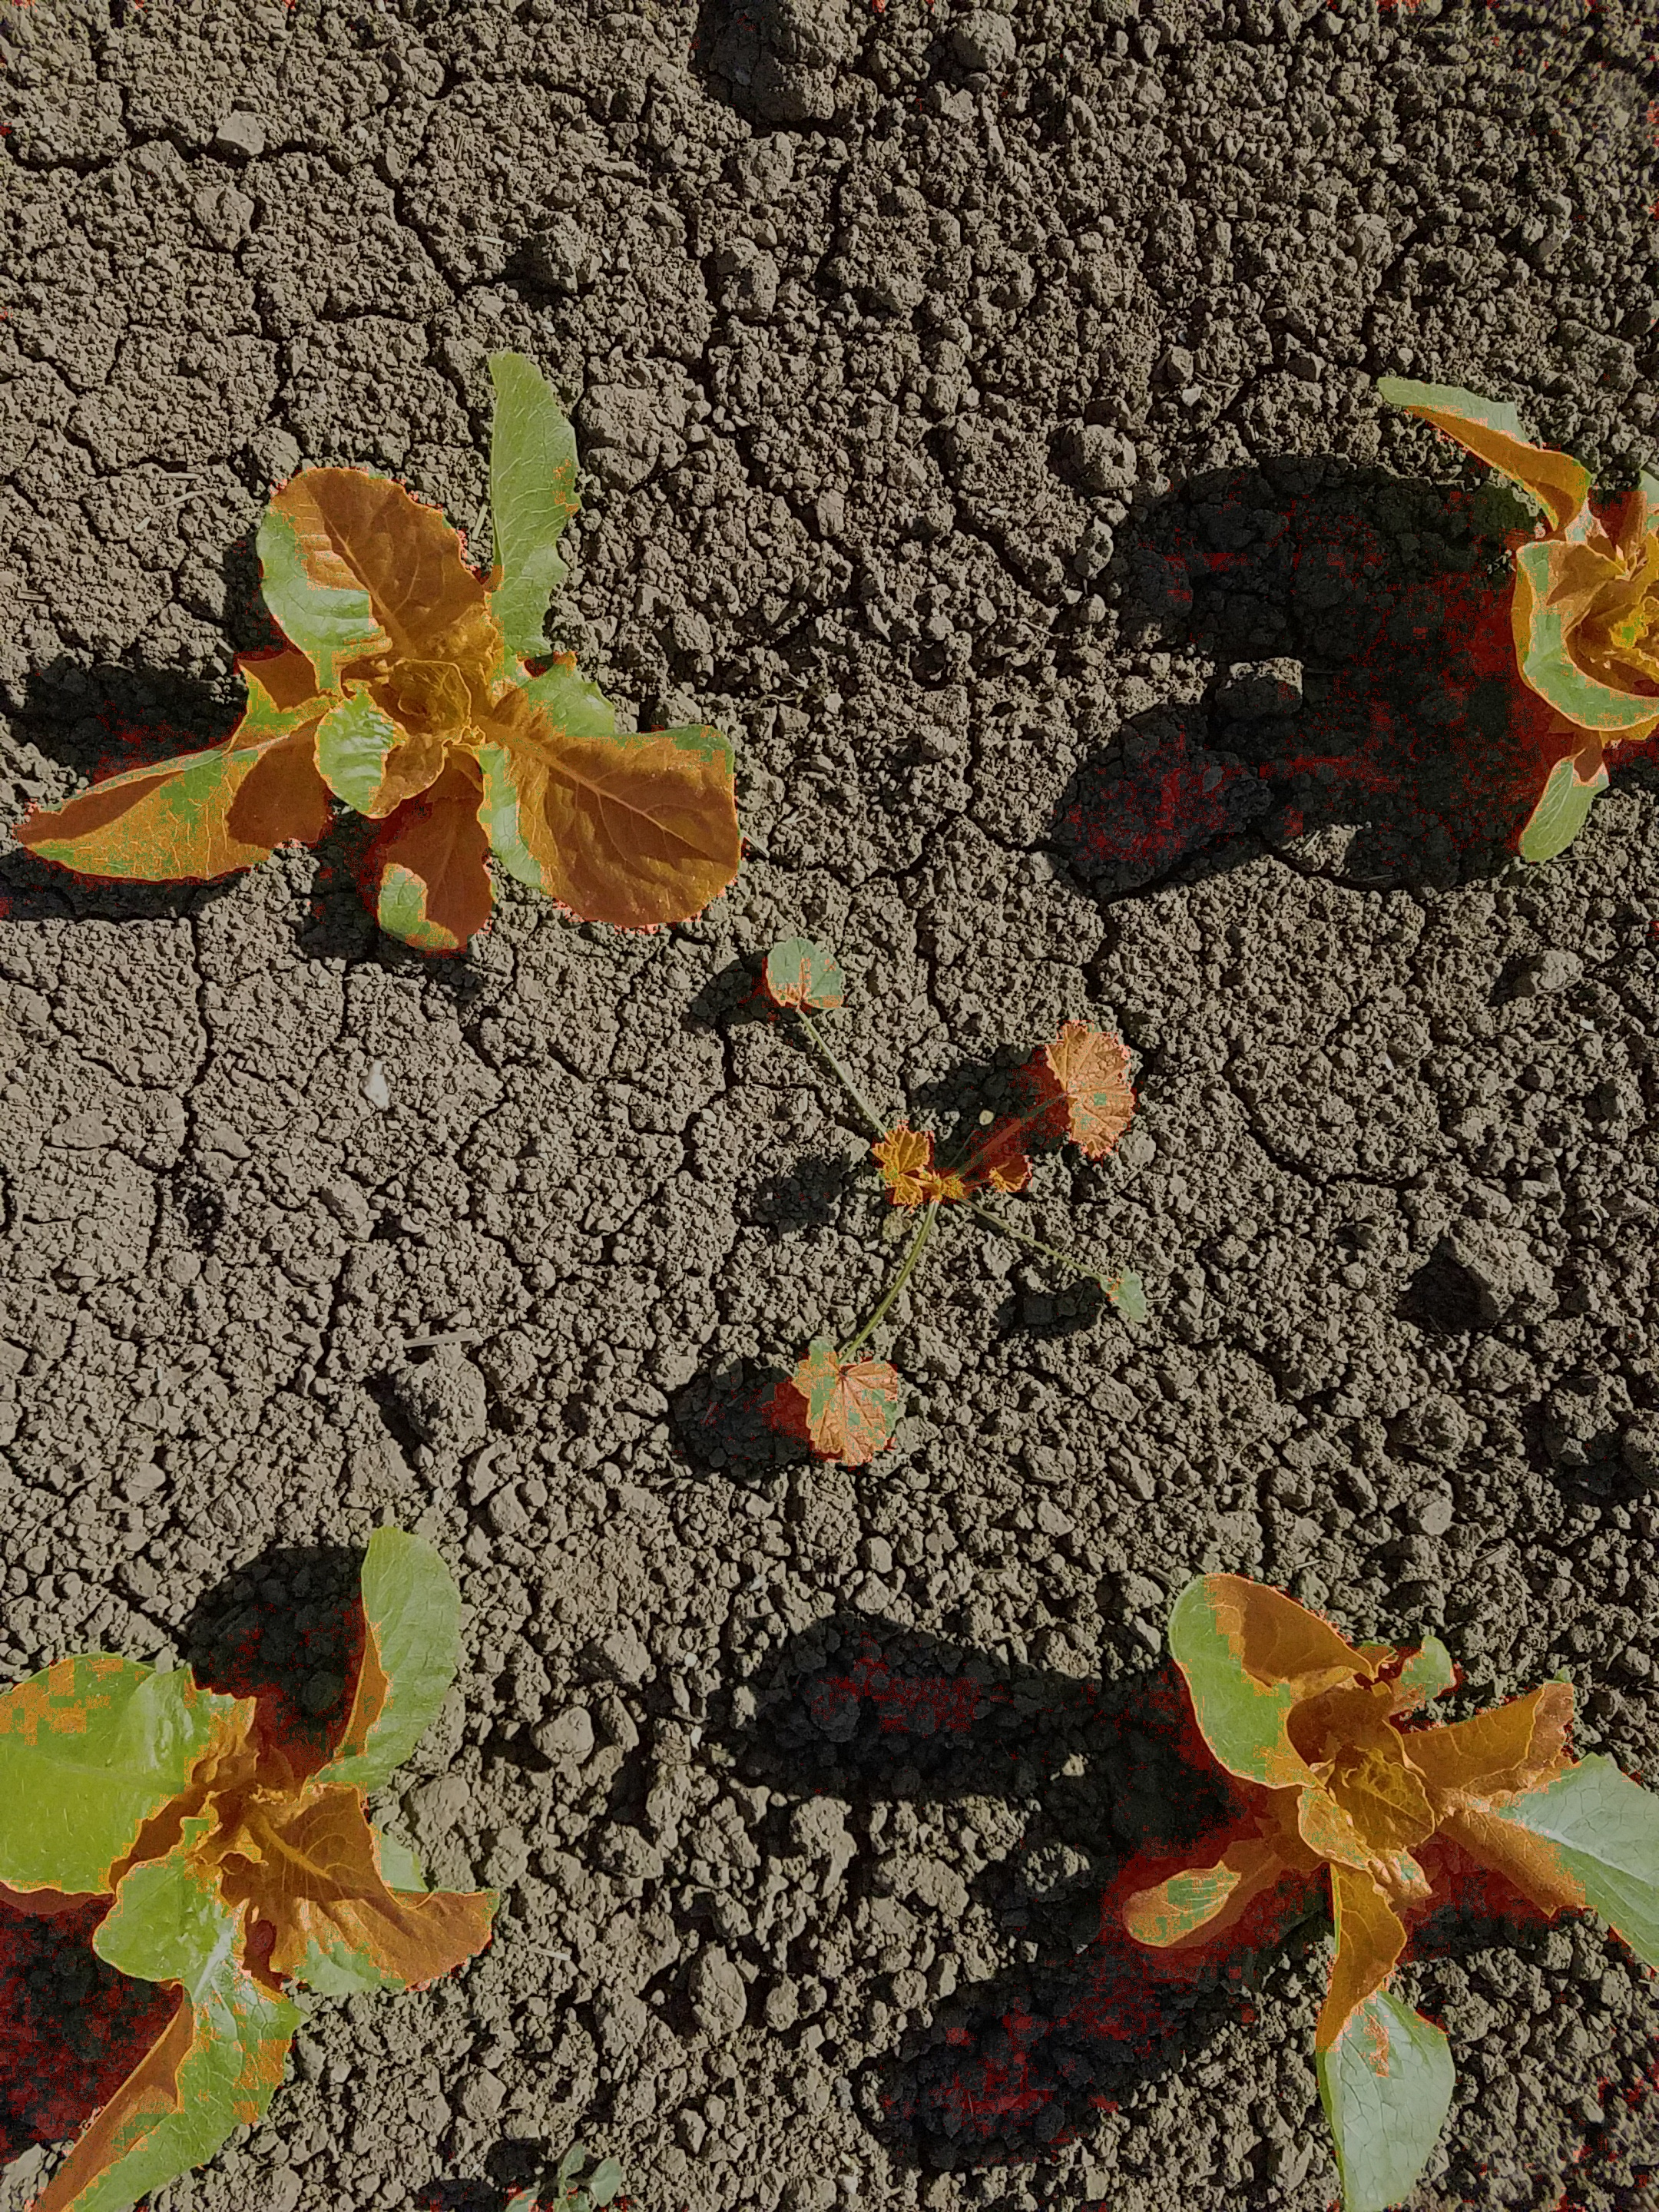
\includegraphics[width=0.45\textwidth]{figures/overlay-ndi.jpg}\label{fig:overlay-ndi}}
	\caption[Masks overlayed on original images]{Masks produced with CIVE and NDI overlayed on the original image. In these images, the masks used are colored red and blended with the original image. Areas that are tinted red will be shown, so a `correct' mask will completely cover vegetation. Note the mask shown in \ref{fig:overlay-ndi} does not cover the plant completely, and segments out shadow portions of the image. What seems to be going on here is that sunlight is shining through the leaf, making the ground green enough to be interpreted as vegetation. Contrast this with the errors seen in \ref{fig:overlay-cive}, where portions of the ground are incorrectly segmented as vegetation in cases not attributable to color contamination. (The upper right-hand portion of \ref{fig:overlay-cive} is a good example of this error.) Photo: Dr. Mark Seimens, University of Arizona.}
	\label{fig:overlay}
\end{figure}

\subsubsection{HSI and HSV}
The Hue, Saturation and Intensity (HSI) and Hue Saturation and Value (HSV) color spaces present an opportunity to consider how saturated the colors are instead of just emphasizing the green found it an image. While that is a bit of an over-simplification of basing a technique on the values found within the RGB bands, it is essentially what is happening. Hue based approaches take much the same approach in one respect -- the hue frequently present in vegetation (green) is represented as peaking around $120^o$ in both models. This is convenient, certainly, as simply considering points as vegetation of they contain hue values around the peak. How wide this range is, of course, will determine what is captured. And while the topic of color is revisited in Section ~\ref{section:problems-color}, consider that leaves contain much that is not green, just as the ground contains much that is not brown. A leaf may contain hue values in the range of 40-70, an indication that the hue is toward the red end of the representation. Likewise, a patch of dirt may contain hue values in the range of 15-20, an indication that the hue is much more red than anything else. HSV is a bit more complicated, in that the V band should be normalized between $(0..1)$ and multiplied by the H value. Lacking more creative terms, these indices will be referred to as HI and HV. 

\begin{equation}
	\label{equation:hsi}
	HSI
    \begin{split}
		discard~pixels~with~H~channel &\geq 190~or \leq 55\\
		discard~pixels~with~S~channel &\leq 0.45 \\
		discard~pixels~with~I~band &\geq 50
    \end{split}
\end{equation}

\begin{equation}
	\label{equation:hsv}
	HSV
	\begin{split}
		H * norm(V) \\
	\end{split}
\end{equation}

\subsubsection{CIELAB}
The CIELAB color space, often referred to with L*A*B* in the name, expresses color along three lines: Lightness (L), Green-Red (A), and Blue-Yellow (B). These values seen in these bands have different ranges, L ranging from 0 (black) to 100 (white), A ranging from negative (green) to positive (red), and B ranging from negative (blue) to positive (yellow). The A and B bands are not technically limited to a specific range, as this space was designed to exceed human perception. Human perception of these colors can be covered with a $\pm 150$ range, and implementations tend to limit the values reported in these bands for pragmatic reasons.  For the purposes of indexing vegetation the bands of  most interest are the A and B bands. Taking the difference between B and A and discarding pixels with a difference is below 30 yields acceptable results. This index will be referred to as CI throughout this document.

\begin{equation}
		\label{equation:cielab}
		B - A, discard~results~\leq~30
\end{equation}

\subsubsection{YCbCr}
This color space (sometimes termed YCC) is frequently encountered in video transmission, as it is designed to address the redundancies seen in the RGB color space. It uses the $Y$ channel to carry Luma information (black and white) and two color channels expressing the blue difference (Cb) and red difference (Cr). Separating the brightness from the color components allows the color representations to match human perception -- as our eyes are more sensitive to changes in brightness than they are to color. As with other indices, the objective is to exaggerate the band vegetation occupies and ignoring components that are not. Using equation \ref{equation:ycbcr} achieves that goal.
\begin{equation}
	\label{equation:ycbcr}
	\ln(Cr) * Cb, discard\ results\geq 890
\end{equation}
This index will be referred to as YCbCRI throughout this document.

\subsubsection{YIQ}
The YIQ model of color was used by the (analog) NTSC color TV system. Later, digital transmission schemes used different color spaces, notably the YCbCr that will be addressed in more detail in a separate section. These schemes have a common approach: \textit{chrominance} (a color component) is added to a black and white image. In the YIQ model, $Y$ represents the luma information (black and white), with $I$ (in-phase, representing red-cyan contrast) and $Q$ (quadature, representing magenta-green contrast) the chrominance information. 
The processing employed here is to convert the image to the YIQ color space and take the mean value for the $I$, or in-phase component for the blob's pixels. (\cite{MathWorks_undated-jg}) For segmentation purposes, the information in the Q band is helpful, primarily in discarding things that are not vegetation.
\begin{equation}
	\label{equation:yiq}
	discard\ any\ pixel\ with\ Q\ band\leq 0.04
\end{equation}
This index will be referred to as YI throughout this document.

\begin{figure}[H]
\centering
\begin{tabular}{ccc}
	\subfloat[CIElab]{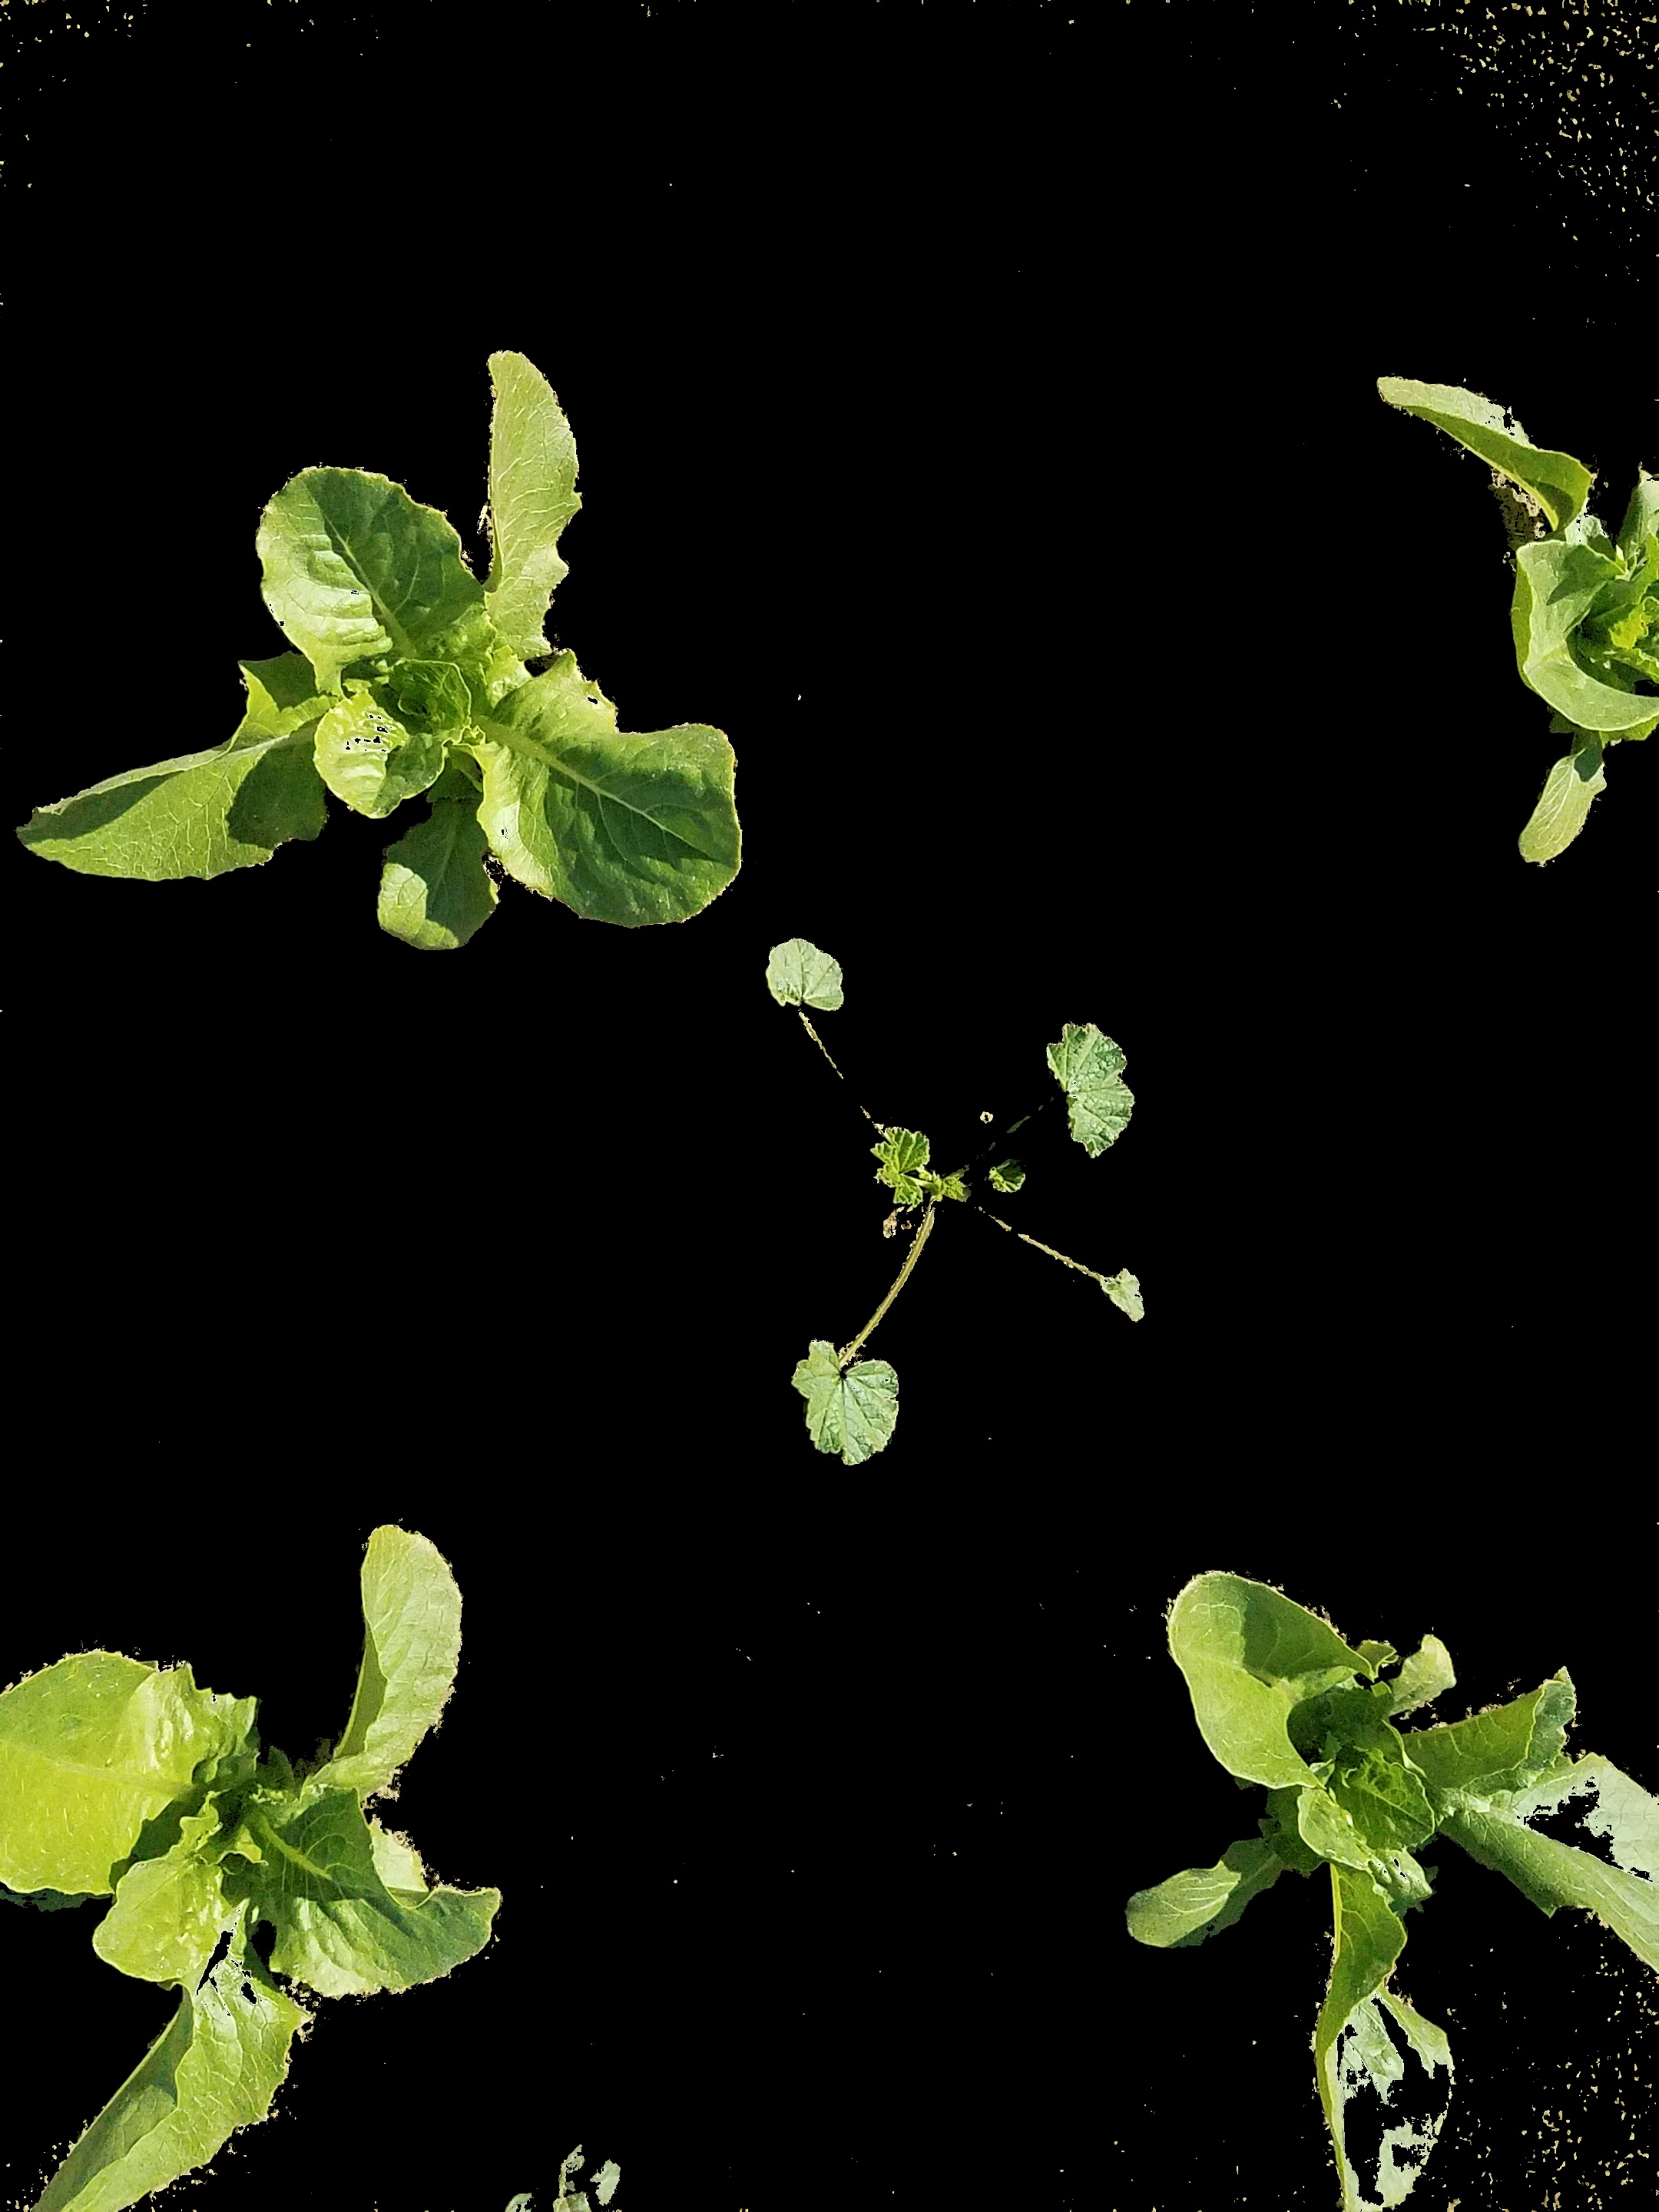
\includegraphics[width = 1.25in]{figures/20201117_112624-CI.jpg} \label{fig:ci}} &
	\subfloat[HSI]{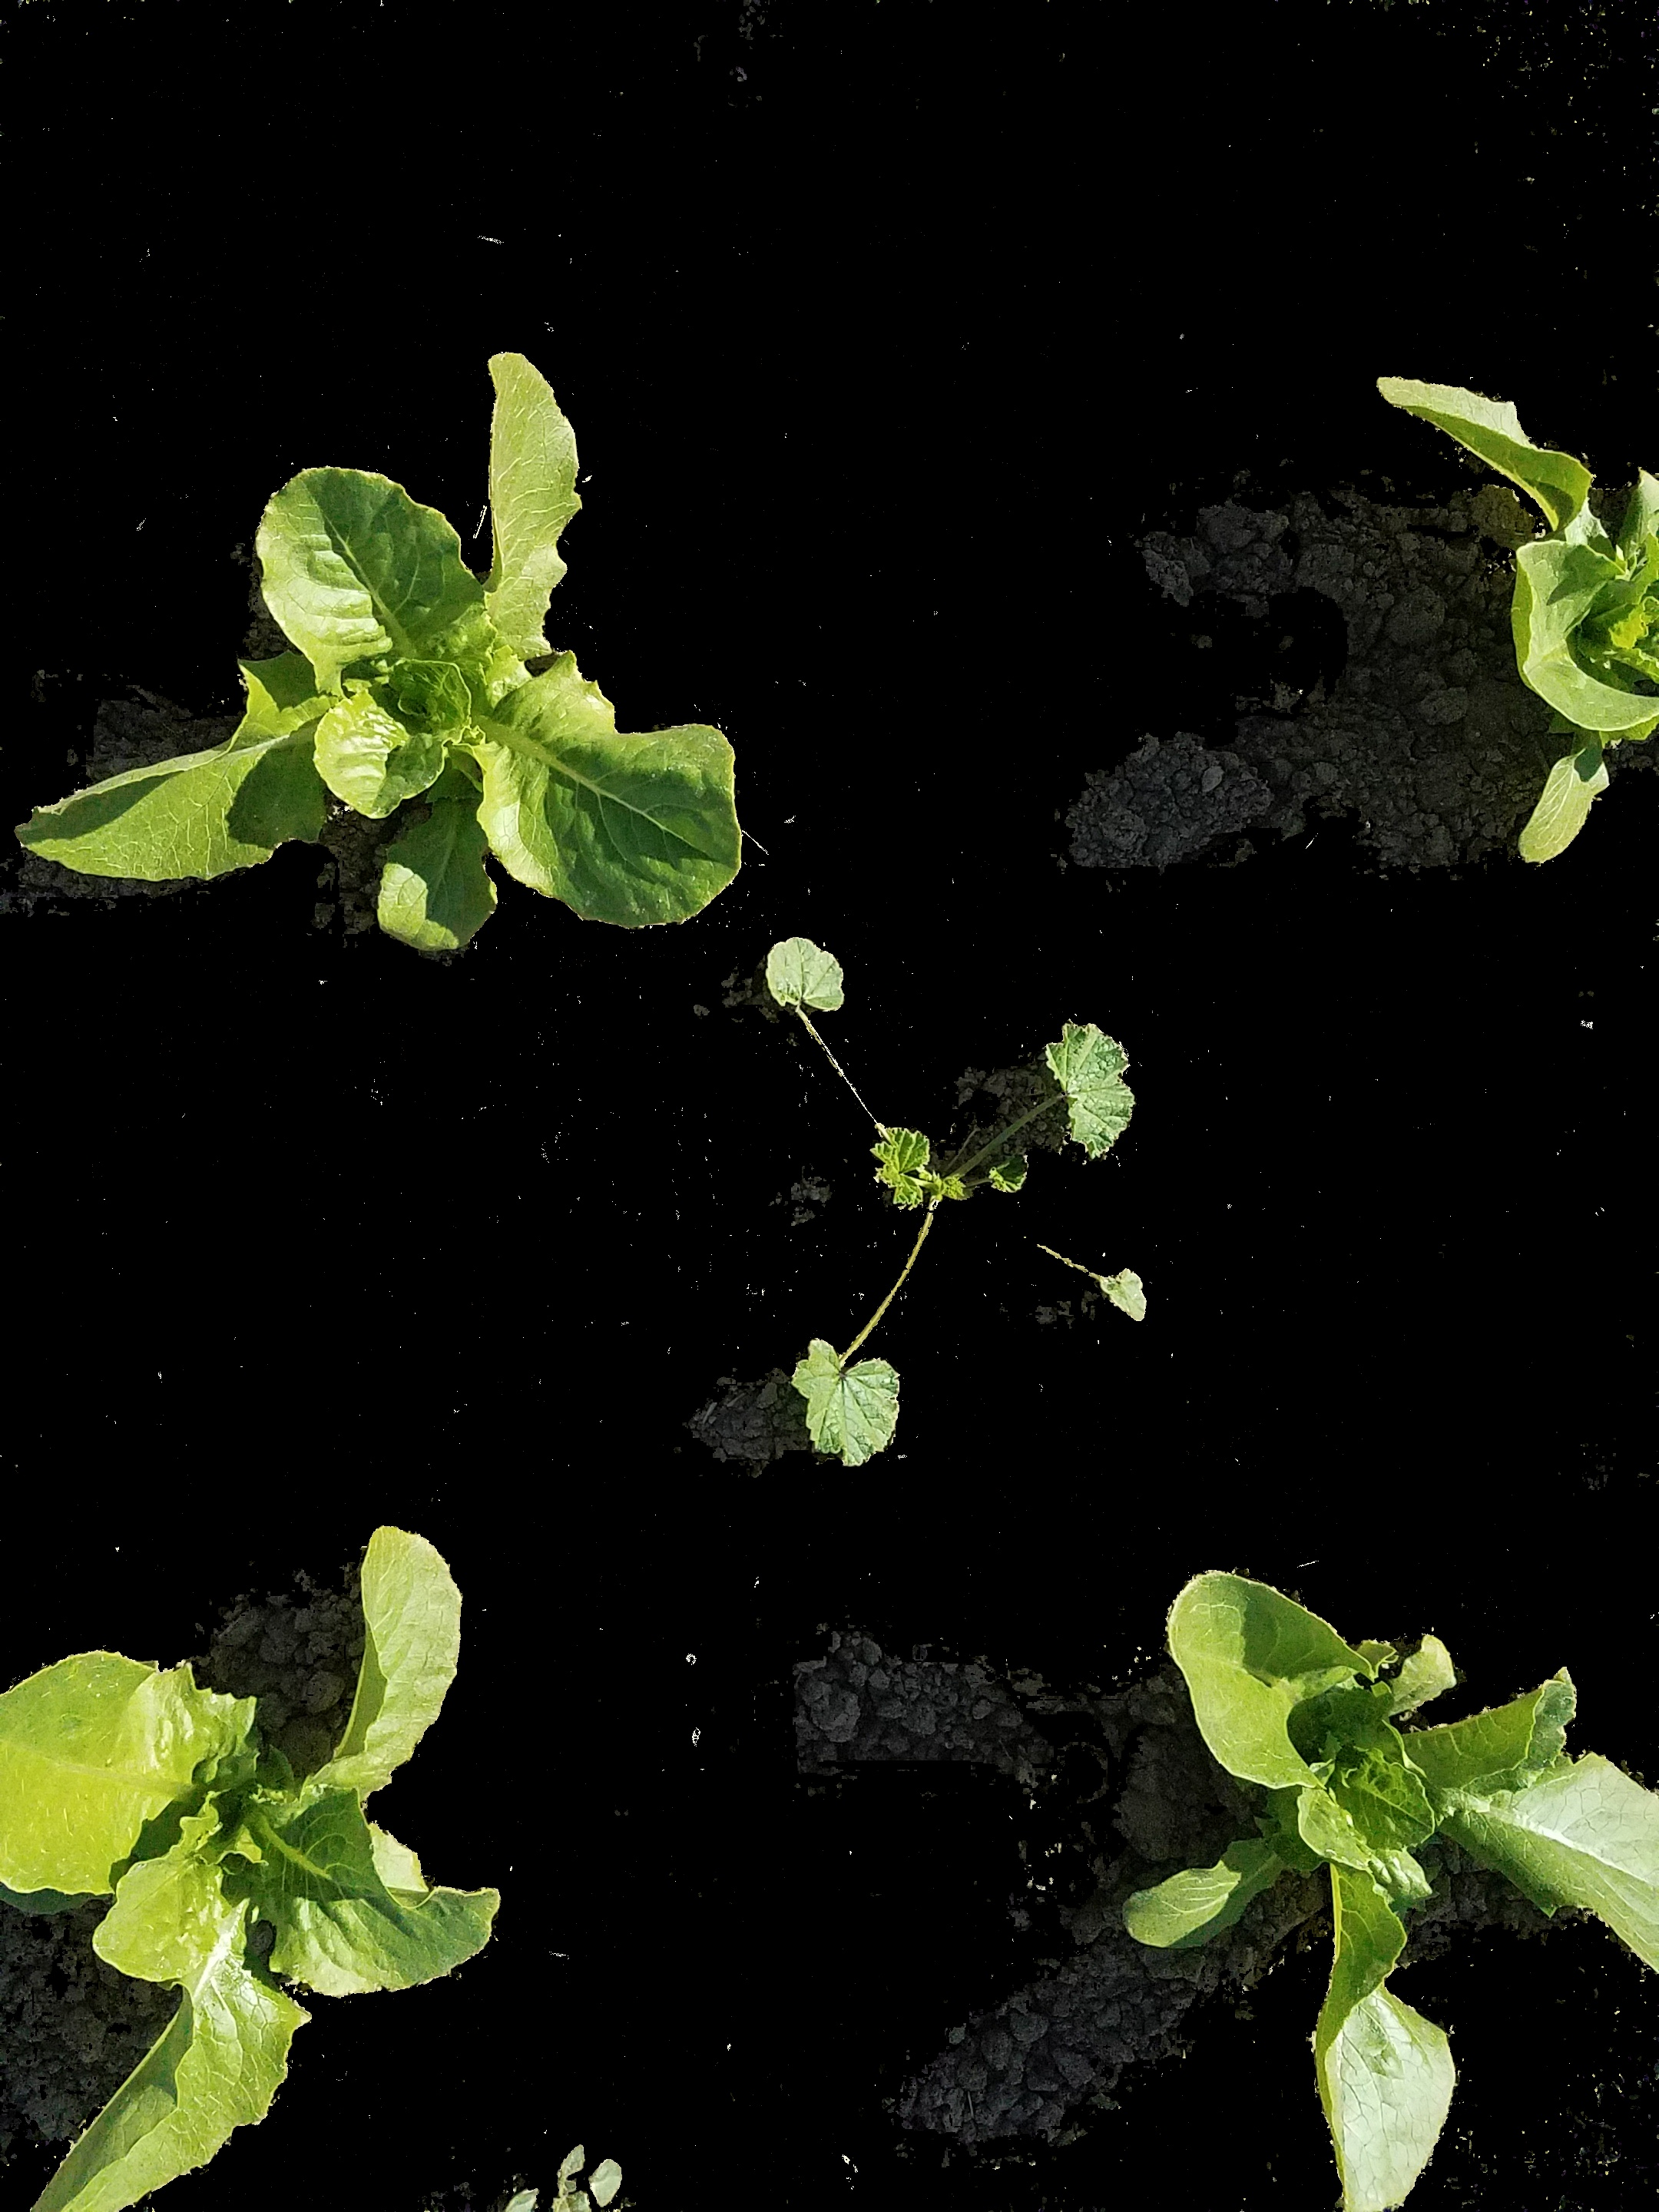
\includegraphics[width = 1.25in]{figures/20201117_112624-HI.jpg} \label{fig:hi}} &
	\subfloat[HSV]{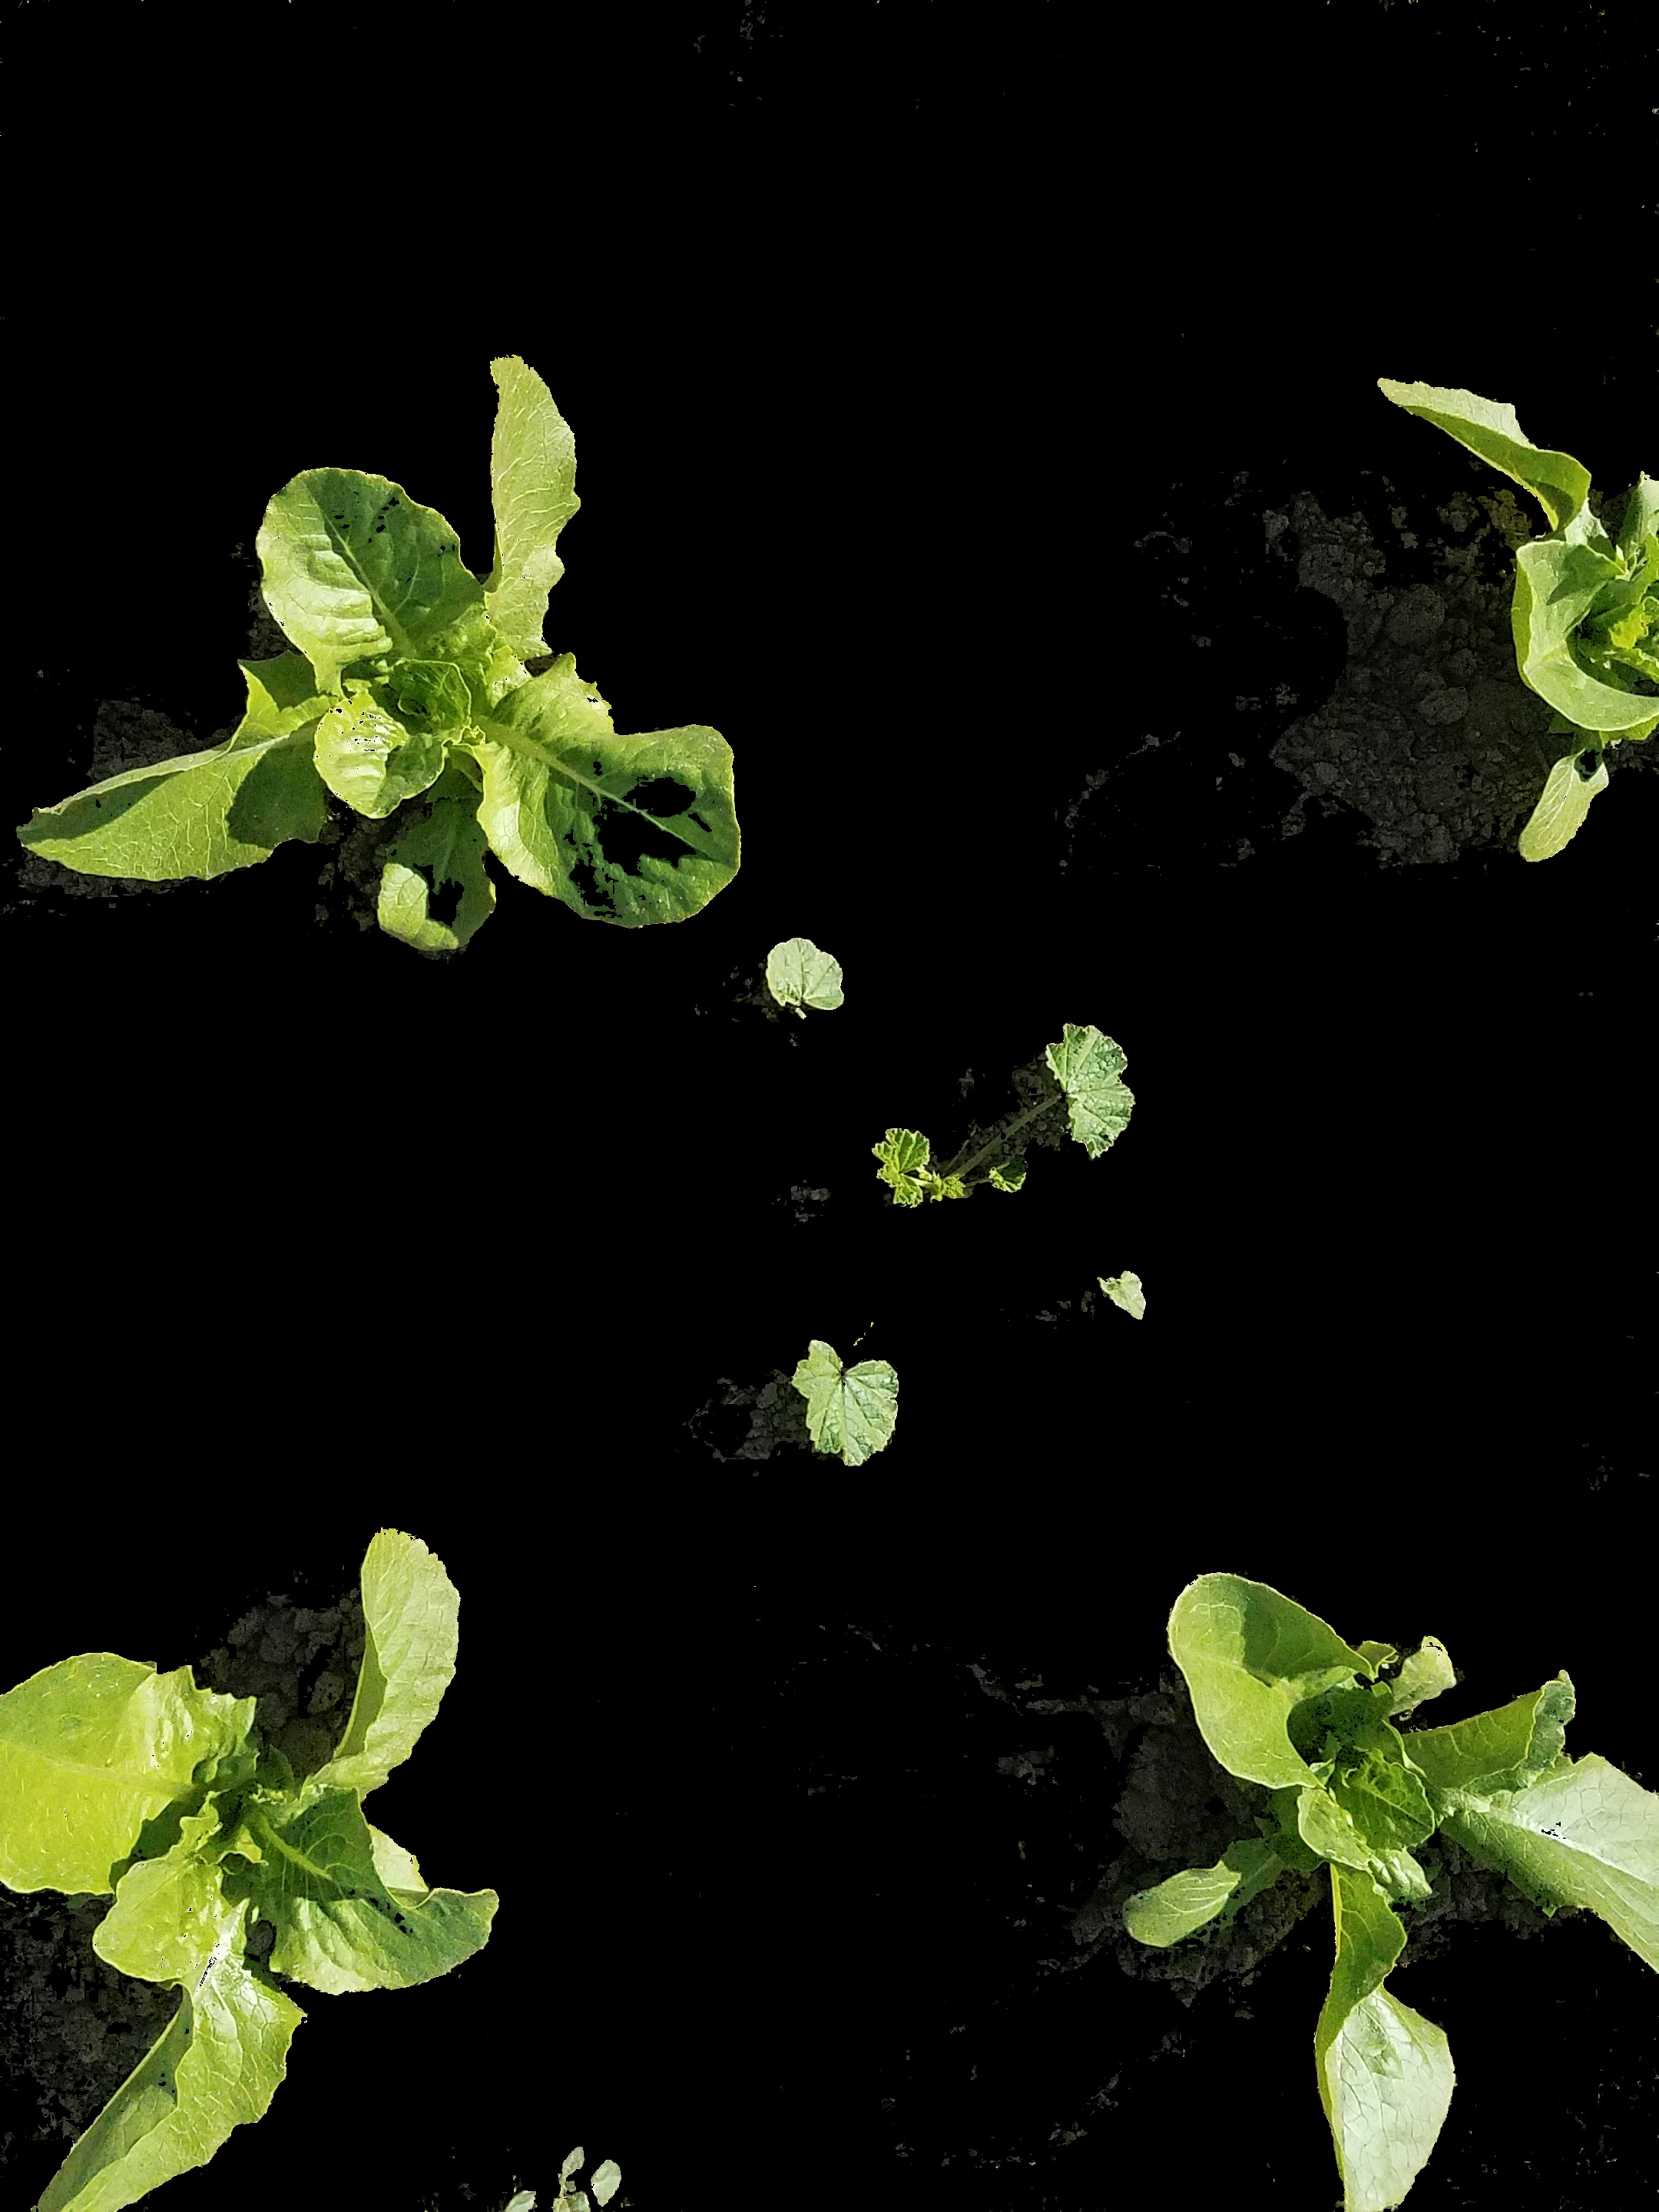
\includegraphics[width = 1.25in]{figures/20201117_112624-HV.jpg} \label{fig:hv}} \\
	\subfloat[YCbCr]{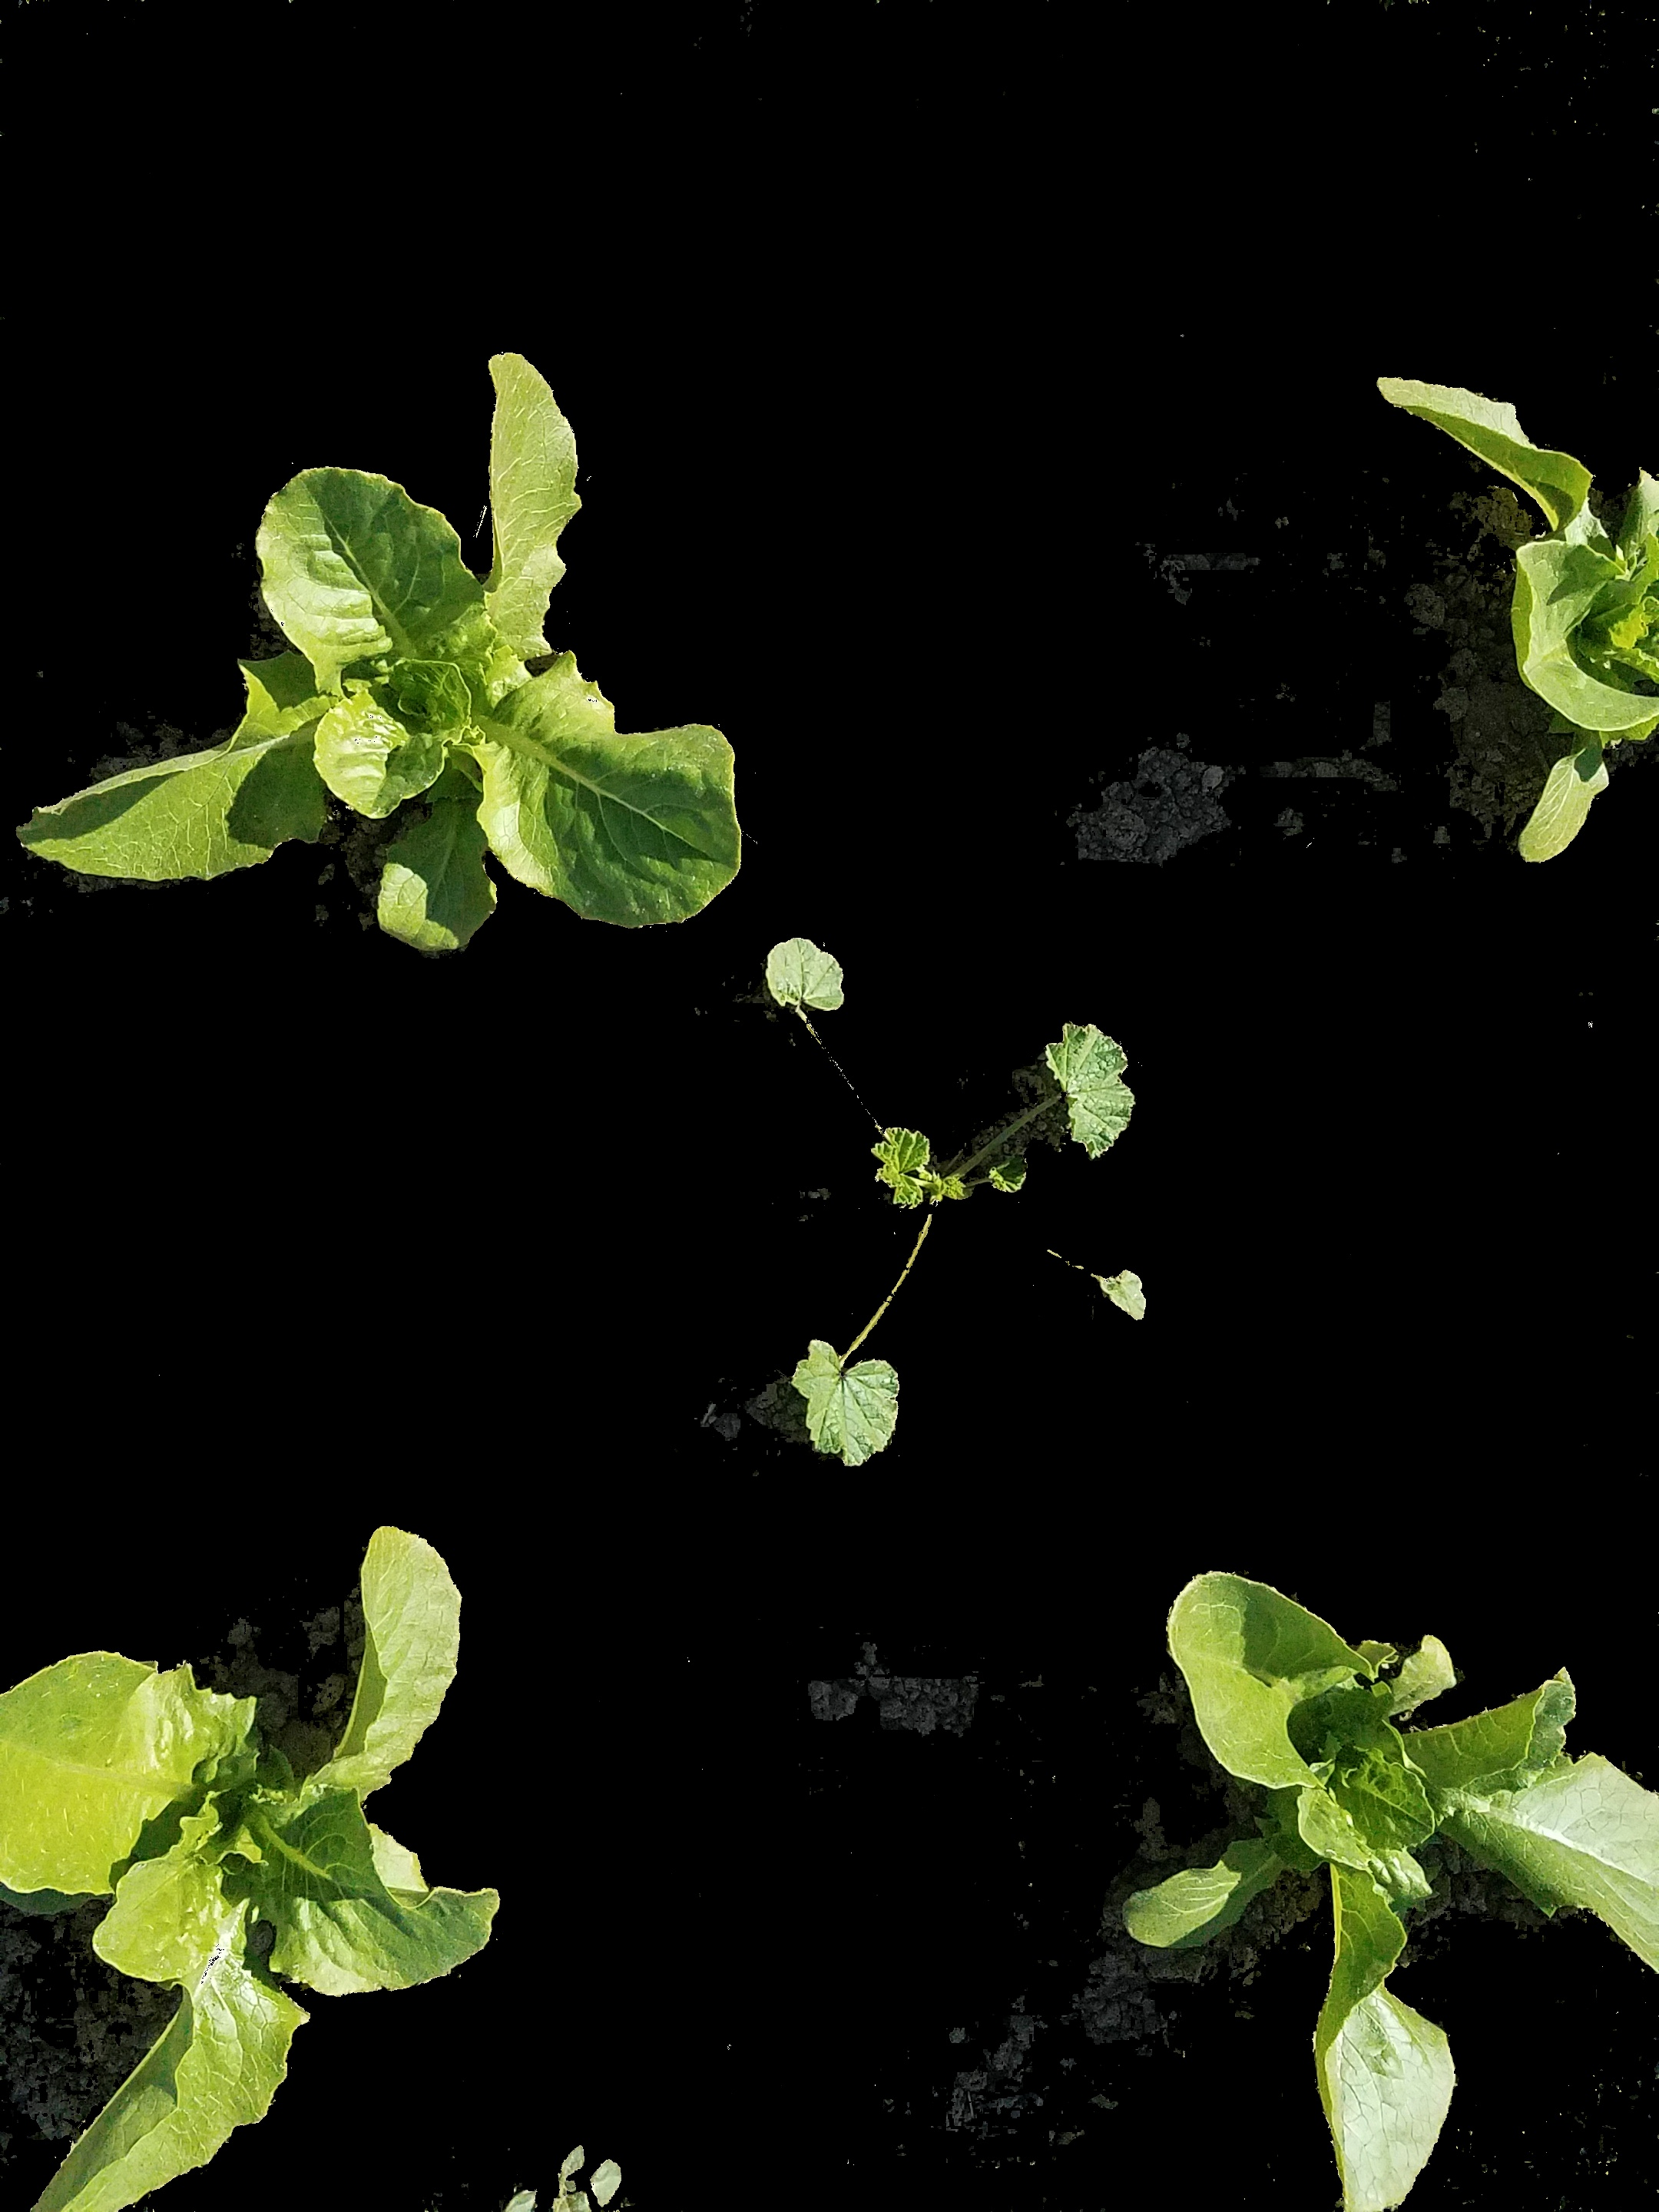
\includegraphics[width = 1.25in]{figures/20201117_112624-YCbCrI.jpg} \label{fig:ycbcr}} &
	\subfloat[YIQ]{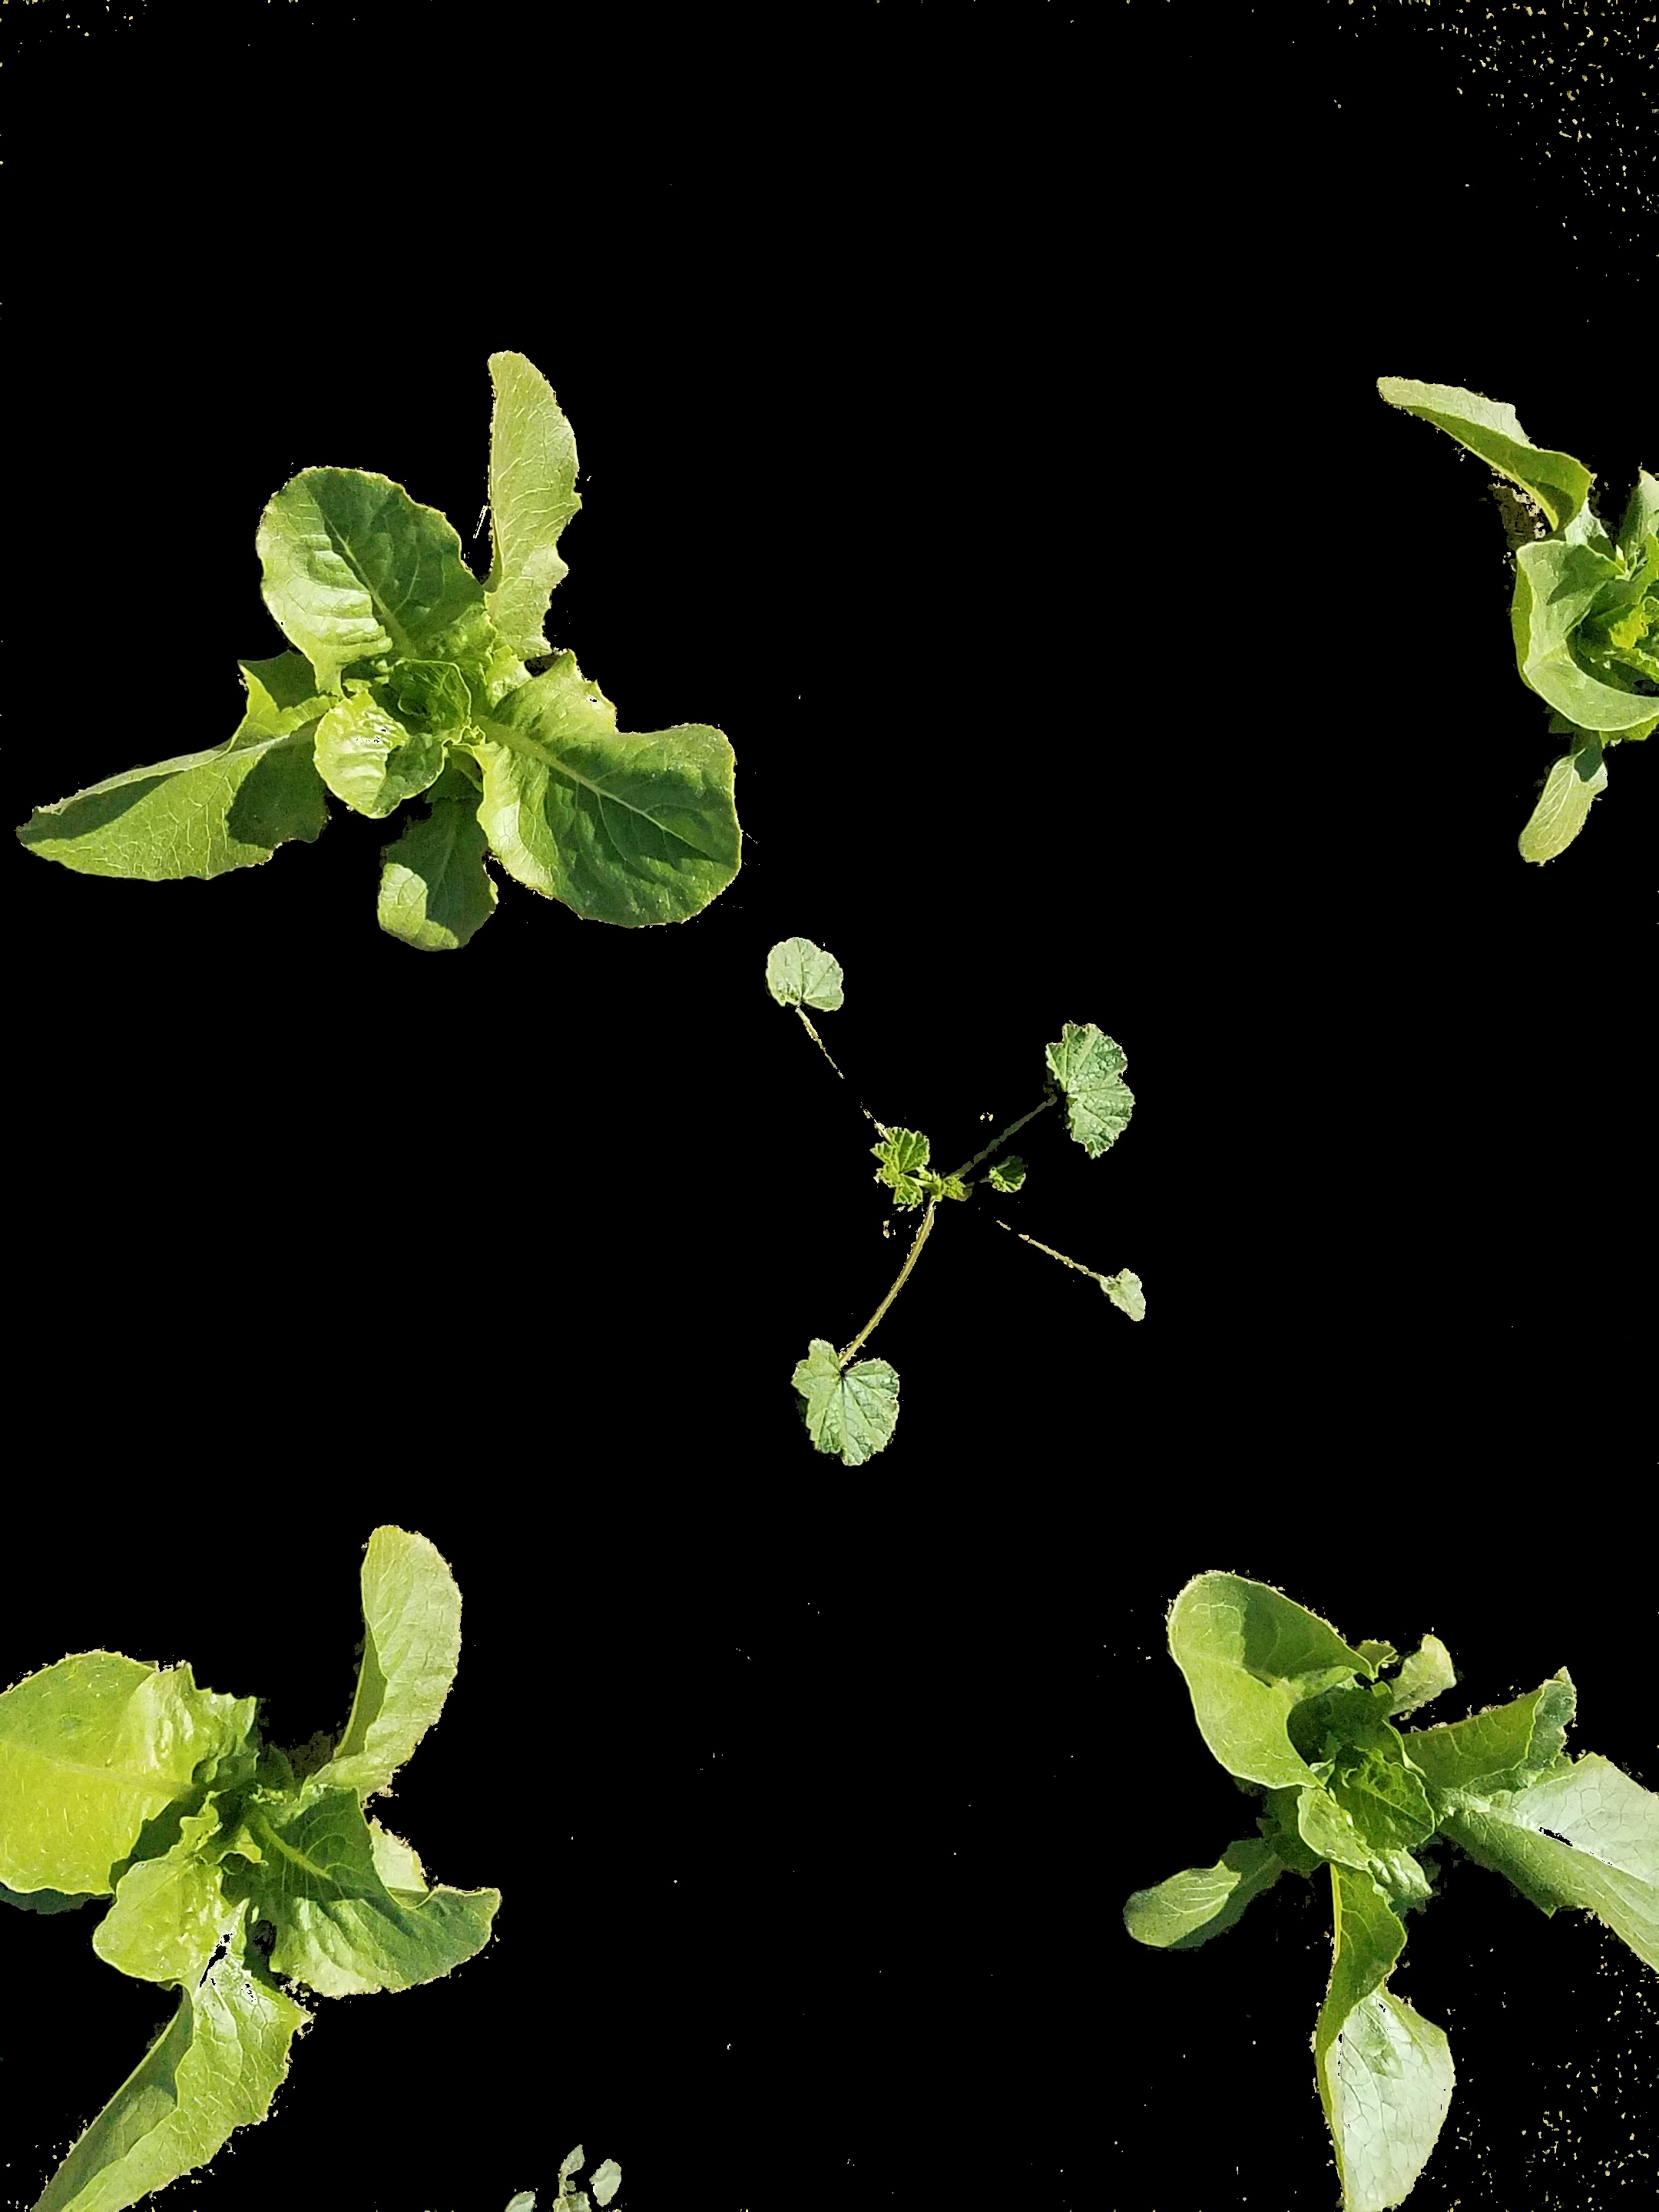
\includegraphics[width = 1.25in]{figures/20201117_112624-YI.jpg} \label{fig:yiq}} &
	\subfloat[Original]{\includegraphics[scale=0.0415,angle=90]{figures/20201117_112624.jpg} \label{fig:original}} \\
	\end{tabular}
	\caption[Segmentation results from various colorspaces outside RGB]{Segmentation results from various colorspaces outside RGB. The \ref{fig:ci} and \ref{fig:yiq} segmentation approaches are relatively clean, providing vegetation images that are free of ground clutter. The other three approaches, while providing good vegetation images, show too much of the ground, particularly in areas near to a plant, likely due to color contamination in the shadow area.}
	\label{figure:results-colorspaces}
\end{figure}

\subsection{Index Evaluation}
Figure \ref{fig:segmentation-errors} shows the error rates encountered with various segmentation techniques, both RGB-centric and those based on other color spaces. Indexing based on the \textit{hue} of the HSI colorspace produced the best results, the \textit{Excessive Red} (based on RGB) index the worst. Curiously, the index based on the other hue-centric color space, HSV, performed significantly worse. There is no one `correct' index approach, of course. It is more a matter of which sort of error can be tolerated within a system. While the HI approached exhibited the best overall error rate, NGRDI might be a better choice if the false positive error rate is a concern. This study will use the NDI and YCbCr index approaches.
 
% Bar chart produced with this command
%  python evaluate-masks.py -i ../lib/mask.jpg -t ../lib/testing/20201117_112624
\begin{figure}[h]
	\centering
	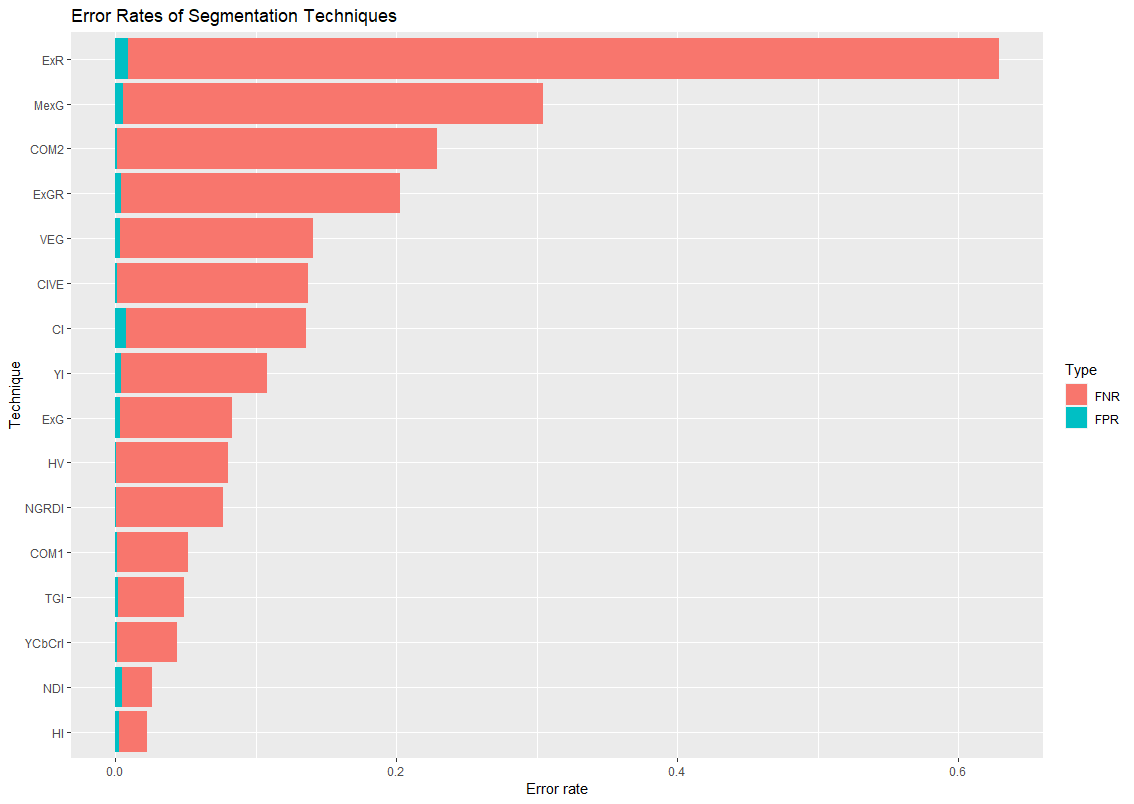
\includegraphics[width=.75\linewidth]{figures/segmentation-error-rates.png}
	\caption[Error rates of segmentation algorithms]{Average error rates for the images. False positive (Vegetation identified as ground) and false negative (Ground identified as vegetation) error are summarized by this figure. Of special note here are the errors encountered with NRGDI and HI approaches, as they represent clear differences in errors. The majority of the errors shown by the HI index mistakenly shows the ground as vegetation, with NDGRI  doing the opposite, hiding vegetation.}
	\label{fig:segmentation-errors}
\end{figure}

\subsubsection{Problem: Reflections and Shadows}
Reflections within vegetation provide a challenge not easily surmounted.  In some cases, the area in reflection is not merely brighter than the surrounding pixels, but is completely devoid of usable pixels, as it is completely white (sometimes referenced as \textit{clipped}). This leads to the situation where portions of the vegetation are not present in the final segmented image, as the pixels do not contain the values associated with vegetation.  Deep shadows suffer from a problem similar to reflections in that they may be seen as nearly pure black. While mild shadows or reflections do not present much of a challenge, as vegetation in these areas typically have pixel values that are closely associated with their class. Reflections and shadows can be partially mitigated by a technique that improves the overall contrast of the image: \textit{histogram equalization}. Histogram equalization, for lack of a more precise description, stretches out the contrast over a broad range. While histogram equalization cannot reconstruct pixels than have been registered as pure white or pure black, this approach yields images with a more uniform intensity distribution.


% This produces figures that have aligned captions -- the [t] bit does the trick
\begin{figure}[H]
	\centering
	\subfloat[Leaf with reflection]{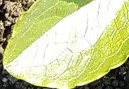
\includegraphics[width=.22\linewidth]{figures/reflection.jpg}\label{fig:leaf-with-reflection}}
	\hfill
	\subfloat[Before]{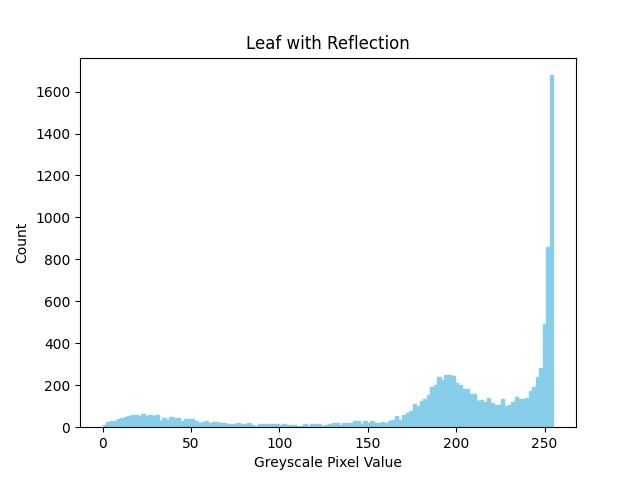
\includegraphics[width=.22\textwidth]{figures/reflection-histogram.jpg}\label{fig:reflection-histogram}}
	\hfill
	\subfloat[After equalization]{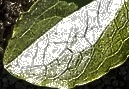
\includegraphics[width=.22\textwidth]{figures/reflection.equalized.jpg}\label{fig:leaf-equalized}}
	\hfill
	\subfloat[After equalization]{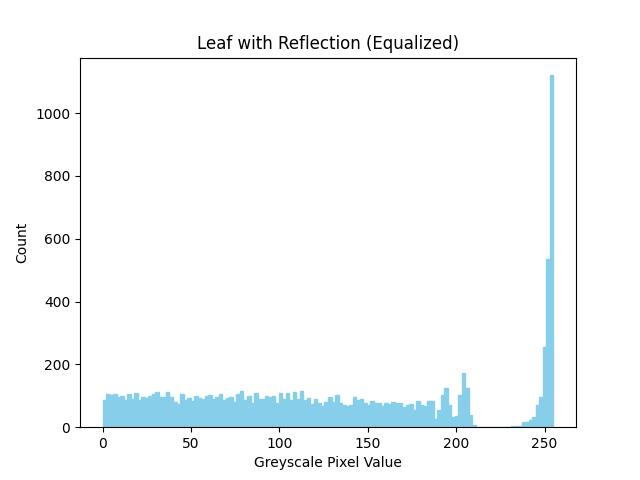
\includegraphics[width=.22\textwidth]{figures/reflection-histogram-equalized.jpg}\label{fig:leaf-equalized-histogram}}
	\caption[Reflection problems in segmented vegetation]{Reflections may be clipped (completely white) containing no usable information. While histogram equalization improves the image somewhat, applying that technique cannot reconstruct pixels that have been recorded as pure white. Figure \ref{fig:leaf-with-reflection} shows a portion of an image with a reflection strong enough to render a significant portion of the image unusable. Note the pixel count for pure or nearly pure white pixels in both \ref{fig:reflection-histogram} and \ref{fig:leaf-equalized-histogram} remain constant.  Those pixels should contain values indicative of vegetation. Aside from being a bit more pleasant to look at, these images differ in way that may have an impact on threshold selection. Note that the histogram of \ref{fig:reflection-histogram} no longer has the same shape, as intensities have be redistributed, eliminating the small bump.}
	\label{fig:reflection}
\end{figure}

\subsubsection{Color problems}
\label{section:problems-color}
Many of the indexes suffer from the same problem: they are focused on vegetation being green. Green stems and leaves are easily detected, but stems and leaves of other colors are not. Consider commonly encountered red-leaf lettuce. Depending on the stage of development and the angle of view, the leaves can be partially or entirely red (or a deep purple color). This is not limited to crops, of course, as weeds such as redroot pigweed (\textit{Amaranthus retroflexus}) have red at the base of the leaves. Likewise, some weeds exhibit red stems. Purslane (\textit{Portulaca oleracea}) has red stems, and as an added complication, red edges on the leaves. Attempts to reveal the stems are complicated by the ground often containing a strong red coloration. Unfortunately, the band of color featured in the stems (red) is frequently found in the background (soil), so attempts to make the stems appear in the masked image are problematic, as this solution tends to bring unwanted ground pixels in the final image that contain hues found within the stems. The result of this is that the non-green portions of the vegetation does not appear in the resulting segmentation.  Even predominately green vegetation has non-green portions. Flowers are often missed by a green-centric index. While the omission of flowers may be desirable in further processing, if the flower obscures green vegetation that would otherwise be identified as such, that complicates further processing, especially when the green portion is significantly obscured. Uncorrected colors also complicate segmentation, as the same plant's leaves may be captured differently with two different cameras or under different lighting conditions. Under controlled lighting conditions (such as would be encountered in an enclosed system) color calibration is not essential every time, but systems that use ambient lighting require calibration each time to achieve optimal results. While the loss of red portions of the plant may not be a significant factor in subsequent processing, this should be taken into account. It may be the case that a single plant appears to be many more, as seen in \ref{fig:ndi}.
There are two other color problems mentioned previously that are worth repeating there. Even green portions of the vegetation may be green ``enough''. The segmented images in Figure \ref{figure:results} have discarded ground pixels while retaining most of the vegetated pixels that will be used is subsequent processing, but a close examination reveals that pixels in the stems of the weed in the center are also eliminated, as they are less green than the rest of the plant. Likewise, immature vegetation where stems are not sufficiently green will not appear in the final image. The color of a pixel may also be ``contaminated'' with color, as shadows or the edges of shadows may contain the color of the vegetation casting the shadow.
Color problems have profoundly negative effects on index accuracy. Figure \ref{fig:segmentation-color-problem} illustrates this on a single image of Purslane. While this may not ultimately result in errors in forming negative treatment plans, as the identification of a single weed as multiple plants, it may have some effects that are not desirable. More herbicide, for instance, may be applied than is required, given that multiple plants are identified where a single plant exists. Even the calculation of weed population is distorted, reporting the incorrect weed count.


\begin{figure}[H]
	\centering
	\subfloat[Field view of Purslane]{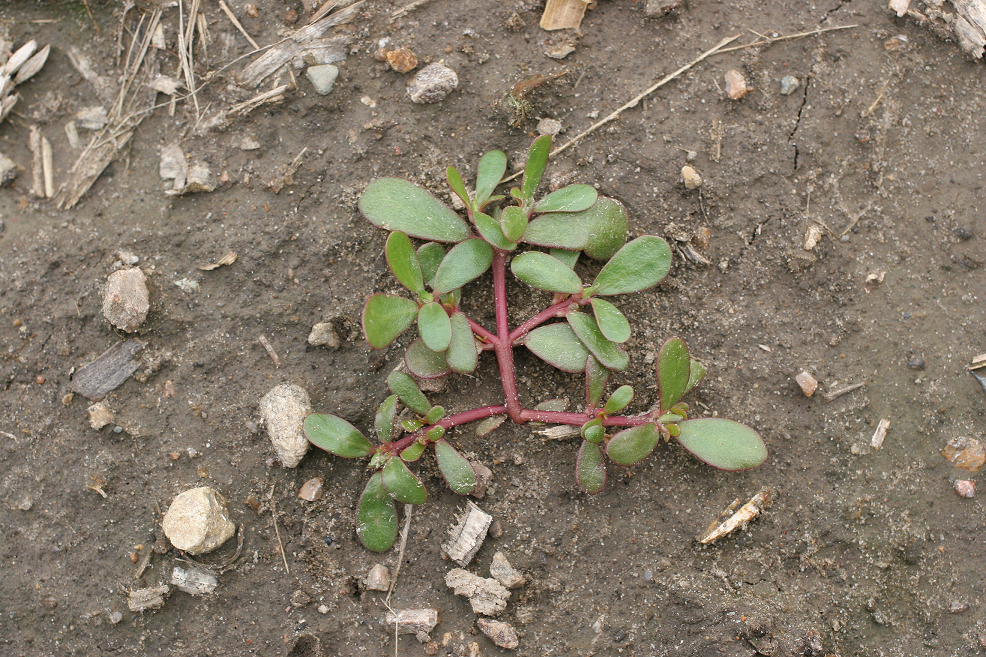
\includegraphics[width=.3\linewidth]{figures/purslane.png}\label{fig:purslane-original}}
	\hfill
	\subfloat[Image processed with NDI]{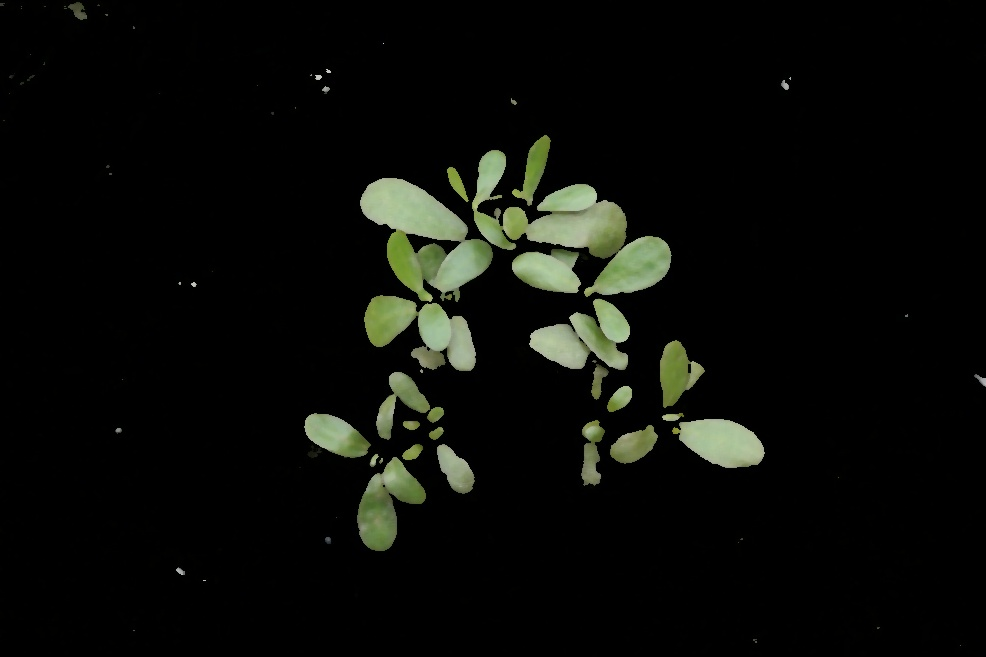
\includegraphics[width=.3\linewidth]{figures/ndi-purslane.jpg}\label{fig:purslane-ndi}}
	\hfill
	% Bar chart produced with this command
	% python evaluate-masks.py -i c:\uofa\weeds\lib\testing\IMG_1133 -s c:\uofa\maricopa\corrected\2024-04-24\iphone-drip\IMG_1133.jpg -t d:\maricopa\masks\2024-04-24\IMG_1133-mask.jpg -l ..\jetson\logging.ini
	\subfloat[Error rates]{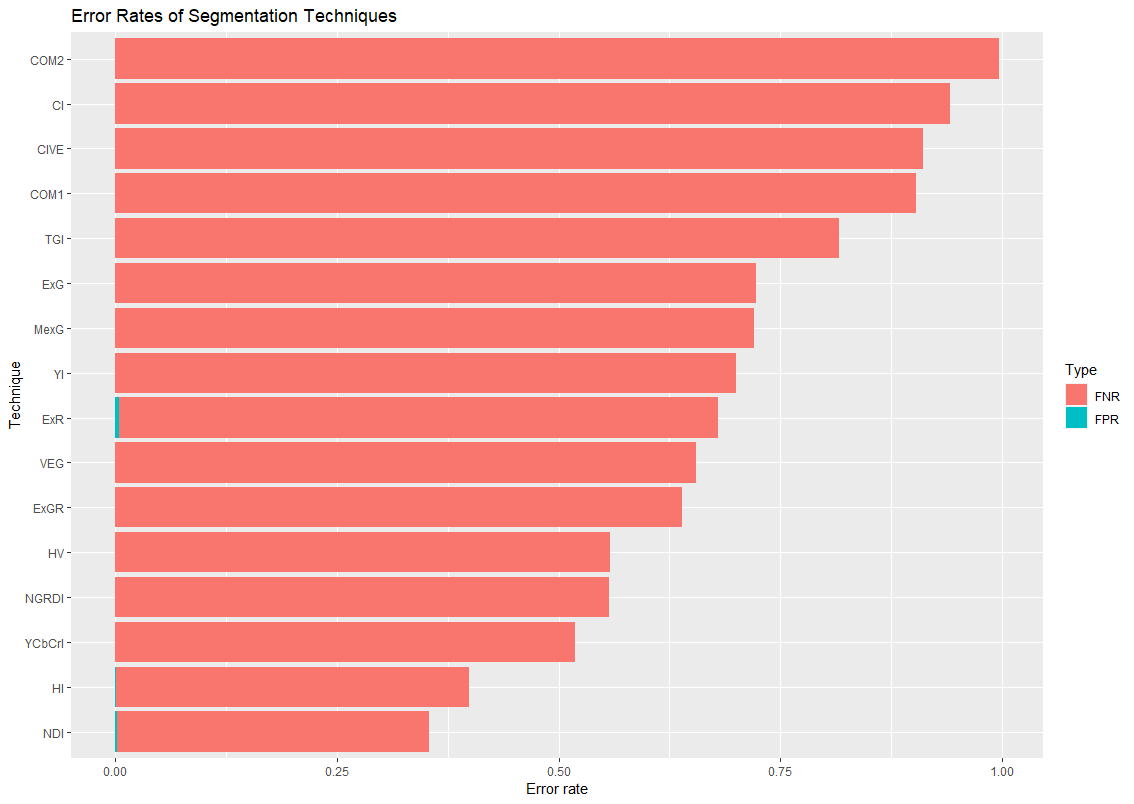
\includegraphics[width=.3\linewidth]{figures/segmentation-error-rates-color.png}\label{fig:error-rates}}
	\caption[Missing red portions of vegetation]{The red portions of the vegetation are missing after the index has been applied, as \ref{fig:purslane-ndi} shows. While the absence of stems may not affect further image processing using factors like leaf texture in classification, the absence of the red portions of features such as leaves may complicate attempts to use factors that are affected such as shape. As \ref{fig:error-rates} shows, the presence of red in a significant portion of the vegetation has a negative impact on the error rates of the algorithms examined.}
	\label{fig:segmentation-color-problem}
\end{figure}

\subsection{Classification Based}
\label{section:classification}
A different approach is to classify each of the pixels in an image as belonging to one of two classes: vegetation or ground (This is often referred to as \textit{semantic segmentation}) Table \ref{table:ml-segmentation} shows the results of building models using the following approaches:  Support Vector Machine, Linear Discriminant Analysis, and Multi-layer Perceptron (MLP)\footnote{These implementations were provided in this \textit{scikit-learn} Python package.}. Each technique was applied to these color spaces: RGB, YIQ, YUV, HSI, HSV, YCbCr, and CIELab. A set of images taken from 2M AGL was selected and 20 samples taken from each of the 58 images, 10 ground points and 10 vegetation points. The term \textit{samples} in this context means that for each of the points sampled, the values for each of the color spaces identified in Section \ref{section:classification} were recorded. Based on these sample points, models were created and trained on 60\% of the data using the Scikit-learn Python library. While the RGB color space is commonly encountered, using it did not produce the best results for any of the techniques examined. That distinction tended to be -- but not always was -- the YIQ space. There are some important exceptions to keep in mind, particularly the performance of LDA, where identical scores for both RGB and YIQ spaces are seen. Using these classification approaches is not particularly pragmatic from a realtime perspective, as classifying every pixel in a modest 12MP image can take several hours on a modestly powerful CPU. Given the poor performance in terms of compute time of this technique, it will not be considered for this project.\footnote{An approach optimized for a GPU would, no doubt, be much faster, but that is an exercise that is beyond the scope of this document.}

\begin{figure}[H]
	\centering
	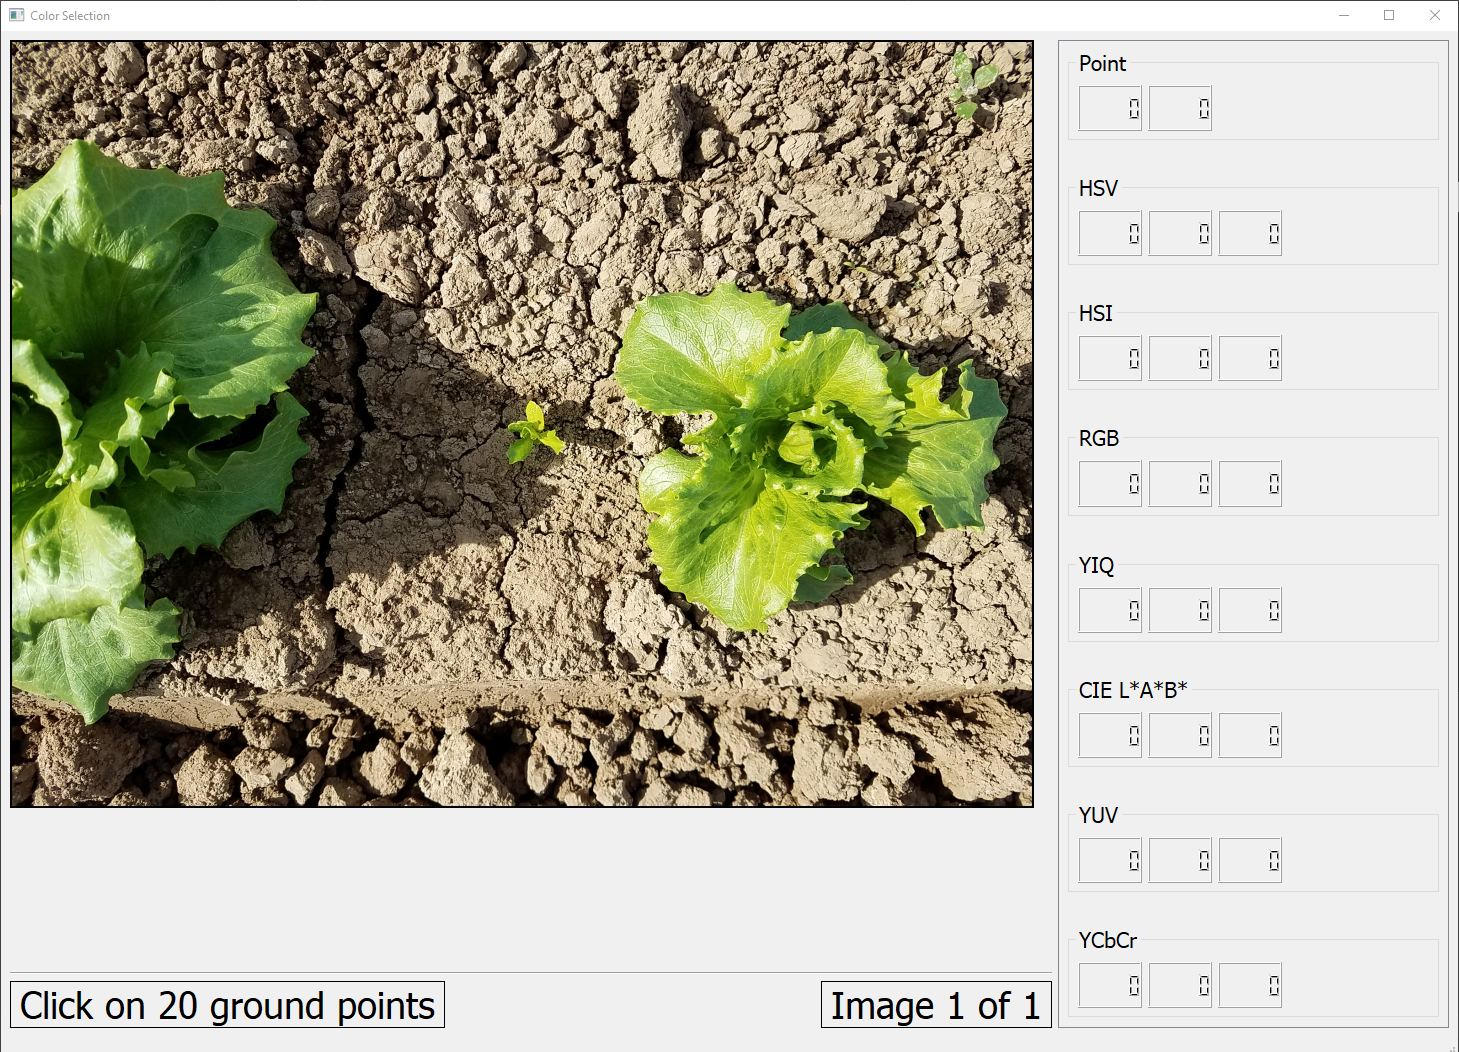
\includegraphics[scale=0.30]{./figures/color-screenshot.png}
	\caption[Color sampling UI]{This application allows a specified number of ground and vegetation points to be sample for each image in a set. The color values along the left-hand side of the interface are simply for debug purposes, not for user interaction. Users simply click on the specified number of ground and vegetation points, and the image automatically advances through the set.}
	\label{fig:color-application}
\end{figure}

%
% Begin Copied Table from this command
% python segment.py -i images -o segmented -t ../util/segmentation-training.csv  -b -s -l logging.ini -a all
% Minor manual edit: Remove leading space from header lines

Table \ref{table:ml-segmentation} shows a summary of the three classification approaches in various color spaces, giving the Area Under the Curve (AUC), Precision, Recall, and F1 scores. And while the the scores reported are encouraging, the resulting segmented images are not.

% Spacing between the rows
{
\renewcommand*{\arraystretch}{0.89}

%
% Begin Copied Table from this command
% python segment.py -i images -o segmented -t ../util/segmentation-training.csv  -b -s -l logging.ini -a all
% Minor manual edit: Remove leading space from header lines & data


\begin{longtable}{llrrrr}
\caption[Machine Learning Segmentation]{Machine Learning Segmentation}
\label{table:ml-segmentation}\\
\toprule
Technique &  Color &  AUC & Precision & Recall &   F1\\
\midrule
\endfirsthead
\caption[]{Machine Learning Segmentation} \\
\toprule
Technique &  Color &  AUC & Precision & Recall &   F1\\
\midrule
\endhead
\midrule
\multicolumn{6}{r}{{Continued on next page}} \\
\midrule
\endfoot

\bottomrule
\endlastfoot
MLP &RGB & 0.93 &      0.88 &   0.95 & 0.91 \\
MLP &YIQ & 0.94 &      0.88 &   0.96 & 0.92 \\
MLP &YUV & 0.94 &      0.88 &   0.96 & 0.92 \\
MLP &HSI & 0.91 &      0.86 &   0.94 & 0.90 \\
MLP &HSV & 0.90 &      0.87 &   0.94 & 0.91 \\
MLP &YCBCR & 0.94 &      0.88 &   0.96 & 0.92 \\
MLP &CIELAB & 0.94 &      0.88 &   0.96 & 0.92 \\
LDA &RGB & 0.94 &      0.88 &   0.96 & 0.92 \\
LDA &YIQ & 0.94 &      0.88 &   0.96 & 0.92 \\
LDA &YUV & 0.94 &      0.88 &   0.96 & 0.92 \\
LDA &HSI & 0.91 &      0.86 &   0.95 & 0.90 \\
LDA &HSV & 0.90 &      0.86 &   0.95 & 0.90 \\
LDA &YCBCR & 0.94 &      0.88 &   0.96 & 0.92 \\
LDA &CIELAB & 0.94 &      0.88 &   0.96 & 0.92 \\
SVM &RGB & 0.94 &      0.89 &   0.96 & 0.92 \\
SVM &YIQ & 0.92 &      0.88 &   0.82 & 0.85 \\
SVM &YUV & 0.93 &      0.86 &   0.93 & 0.89 \\
SVM &HSI & 0.91 &      0.87 &   0.94 & 0.90 \\
SVM &HSV & 0.90 &      0.87 &   0.94 & 0.90 \\
SVM &YCBCR & 0.92 &      0.85 &   0.91 & 0.88 \\
SVM &CIELAB & 0.91 &      0.86 &   0.96 & 0.90 \\
\end{longtable}

% 
% End copied table
%
}

\subsection{Semantic Segmentation}
Semantic segmentation is a convolutional neural network (CNN) using a trained model to classify each pixel in an image with a class label.  For the most part, agricultural images contain only two things: plants and the ground. While there are exceptions to this, of course, as images may include debris on the ground, irrigation equipment, etc., but from another viewpoint, images contain pixels that are plants and pixels that aren't.  The focus here is not to actually classify what each pixel represents (a broccoli plant, a segment of pipe, the ground, etc.), but to produce a mask that can be applied to the image to isolate vegetated pixels. This approach differs from the prior two approaches in that while index-based approaches consider no information about other images, and learning base approaches consider samples of a set of images to predict class membership, the deep-learning techniques considered in this section are trained on both images and the corresponding masks.

\subsubsection{U-Net}
The name of the U-Net architecture derives from the U-shaped arrangement of the downward decoder section and the upward encoder section. Developed initially for the segmentation of bio-medical images \cite{Ronneberger2015-ye}, this technique has been more widely adopted into various use cases.

\begin{figure}[H]
	\centering
	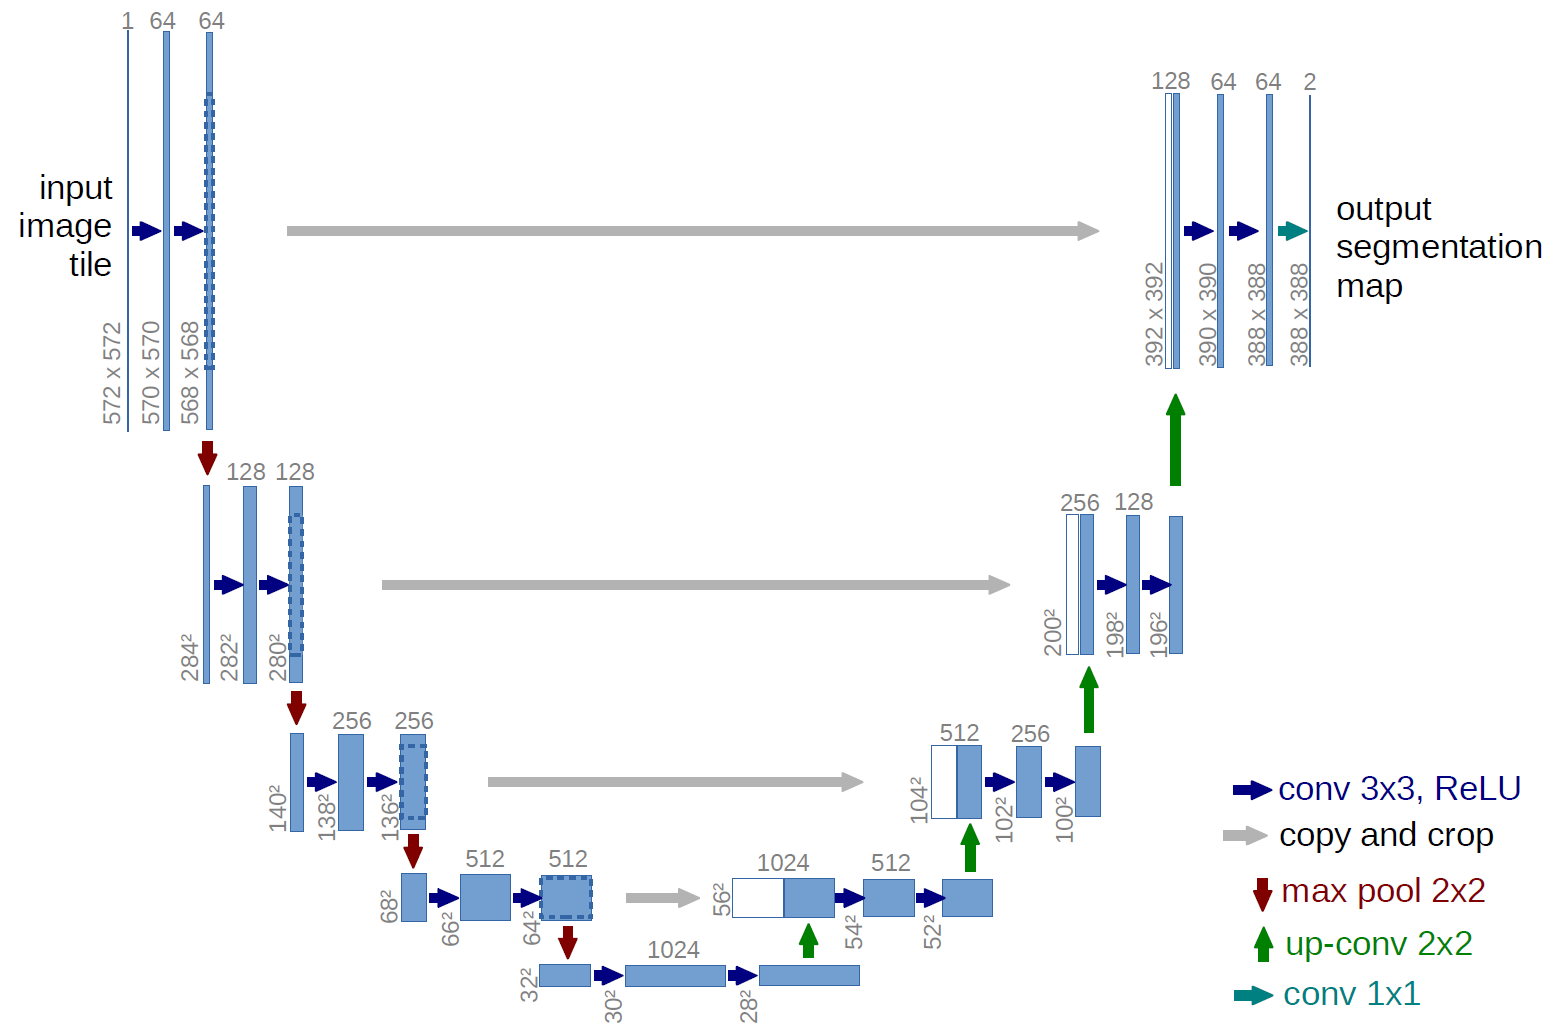
\includegraphics[height=5cm]{figures/u-net-architecture.png}
	\label{fig:u-net}
	\caption[U-Net architecture]{The name of U-Net architecture refers to the arrangement of decoders (often referred to as a contracting path) and encoders (the expanding path)}
\end{figure}
This architecture has a bit of a limitation that must be taken into account in image sets: the length of each image's axis must be a multiple of 16. That is, a 32x32 image will work, but a 32x90 image will not. The images and masked used for training and testing should be resized to fit this limitation. Additionally, the images must be down-sampled to achieve realistically short mask production times. (That is, the images were 1008x752 instead of the original 4032x3024) Using a model trained on images and associated masks from the MAC to a set of test images yields fairly low error rate masks when  those masks are evaluated against the ground truth: FPR of 0.0005 and FNR of 0.06, comparable to the lower rates achieved with some index-based approaches.

\begin{figure}[H]
	\centering
	\subfloat[Ground truth mask]{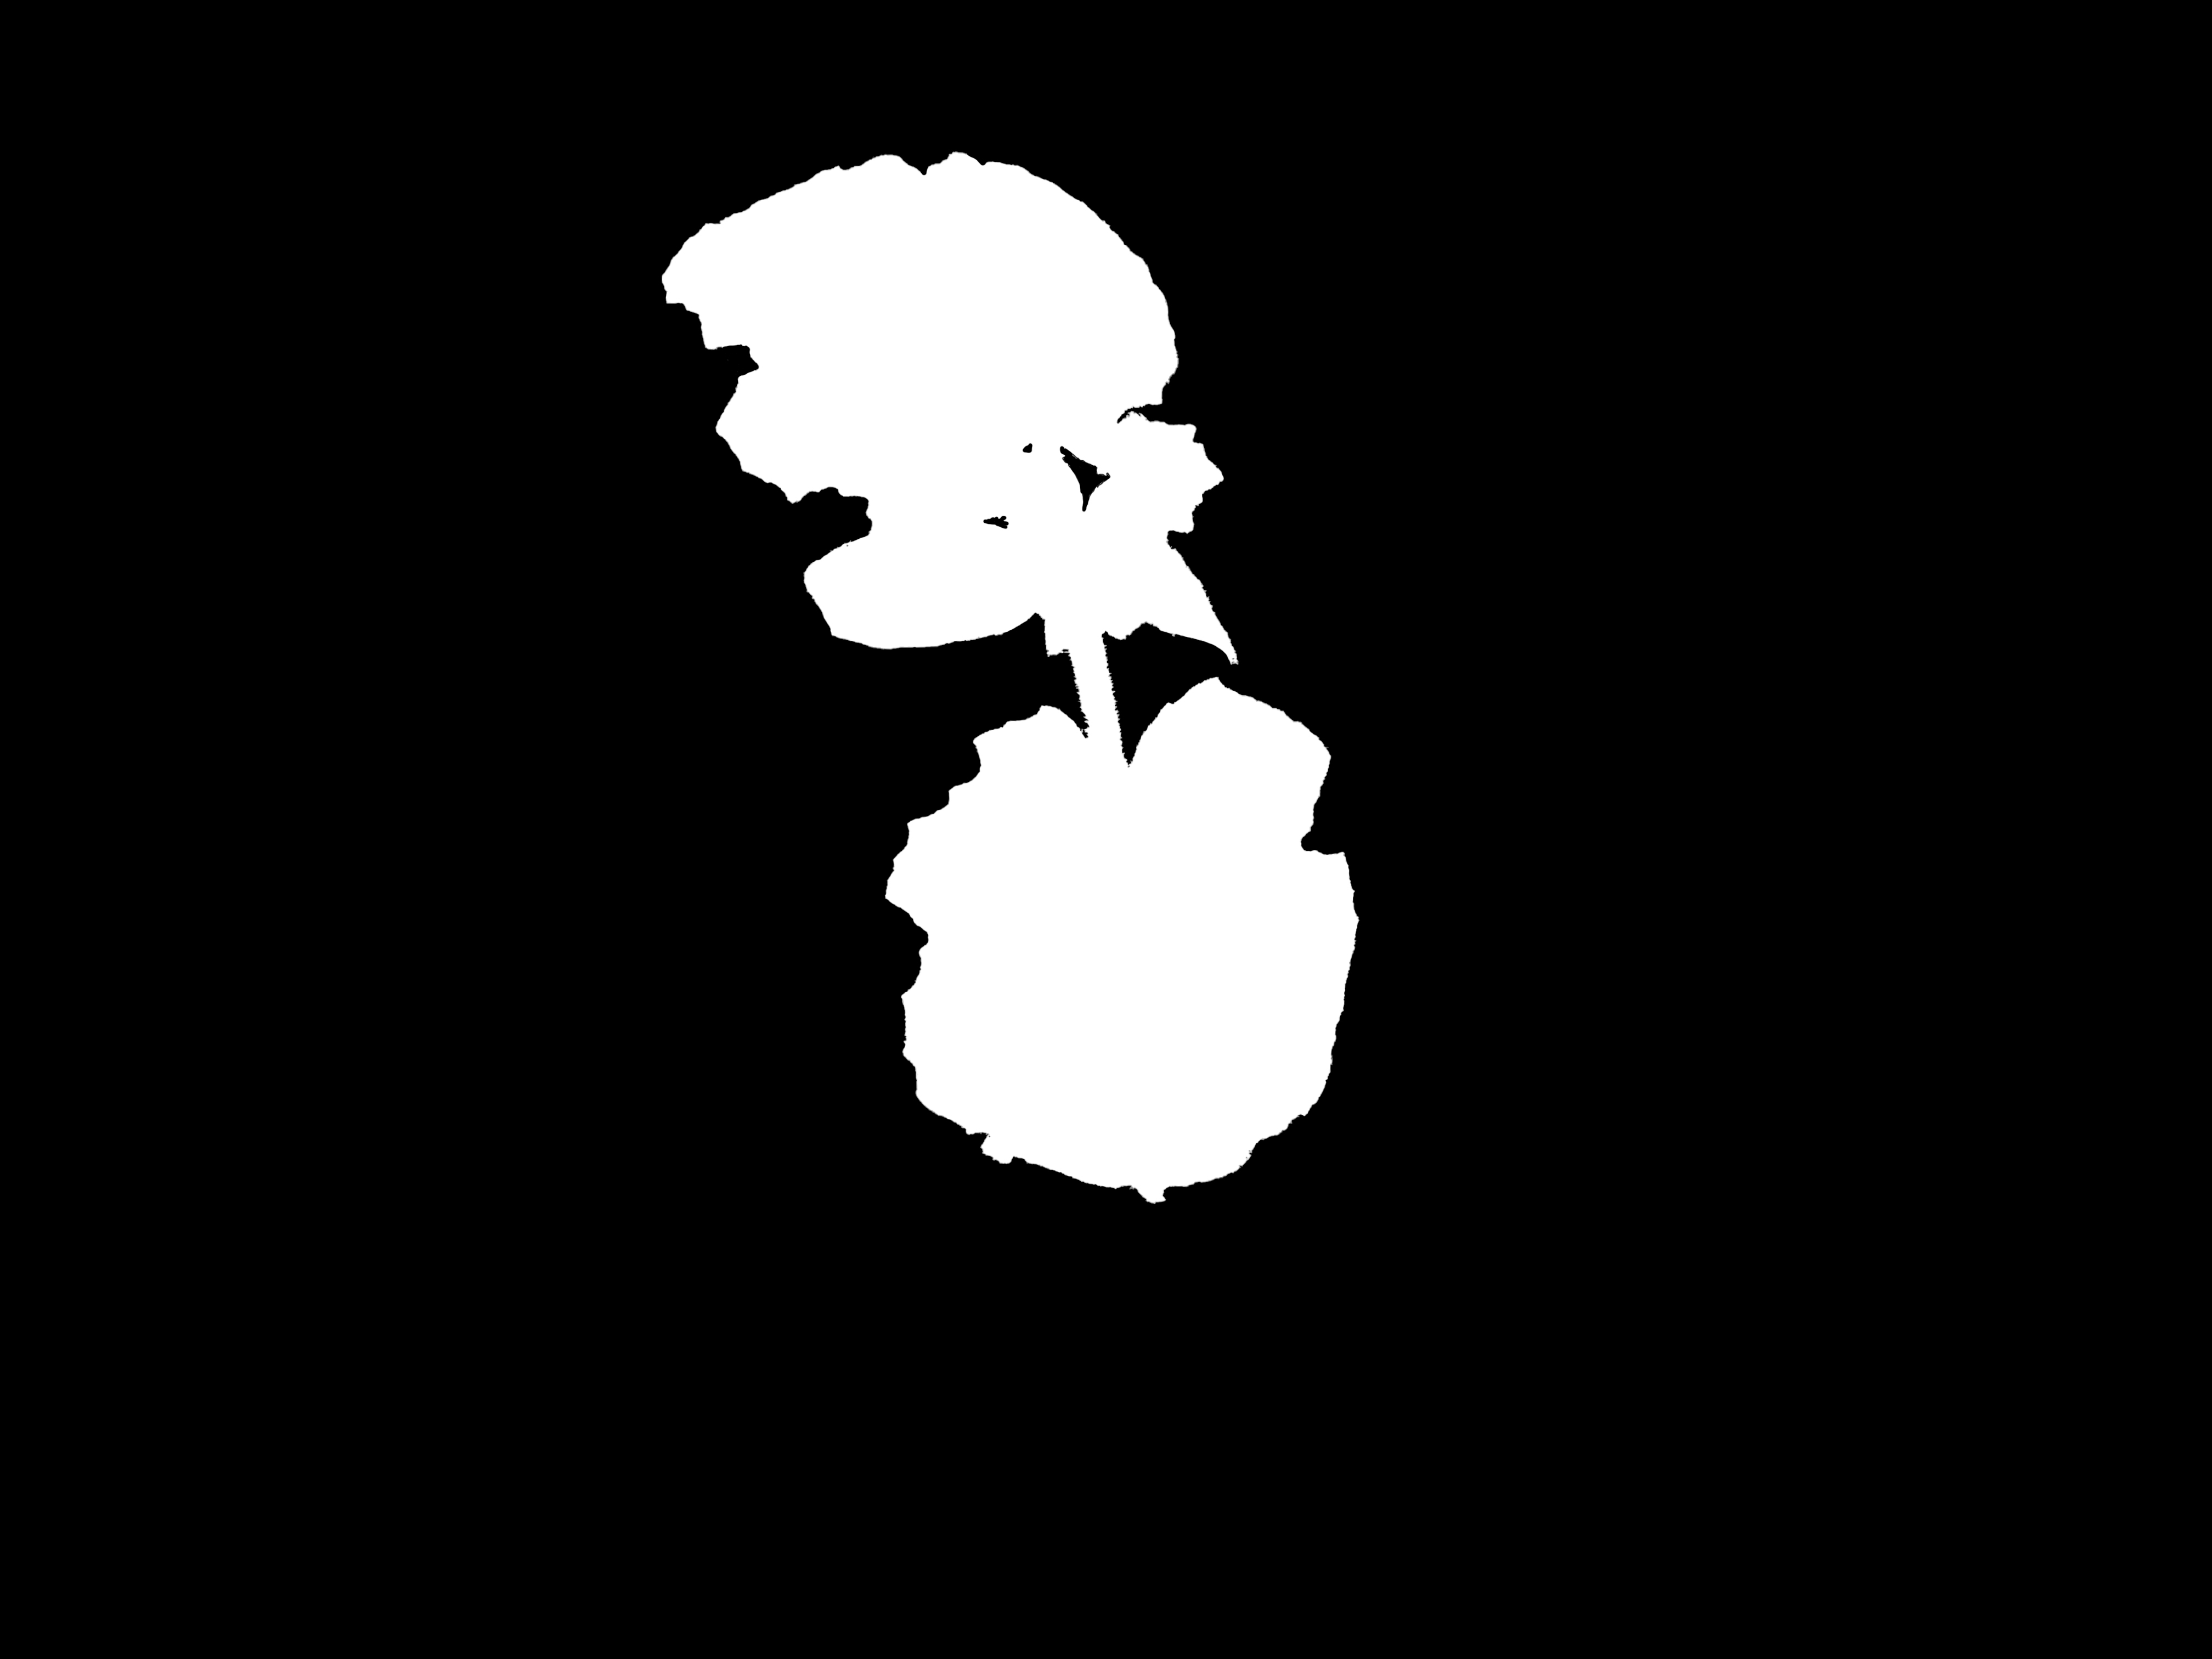
\includegraphics[width=.3\linewidth]{figures/IMG_1115-mask.jpg}}
	\label{fig:unet-original}
	\hfill
	\subfloat[U-Net mask]{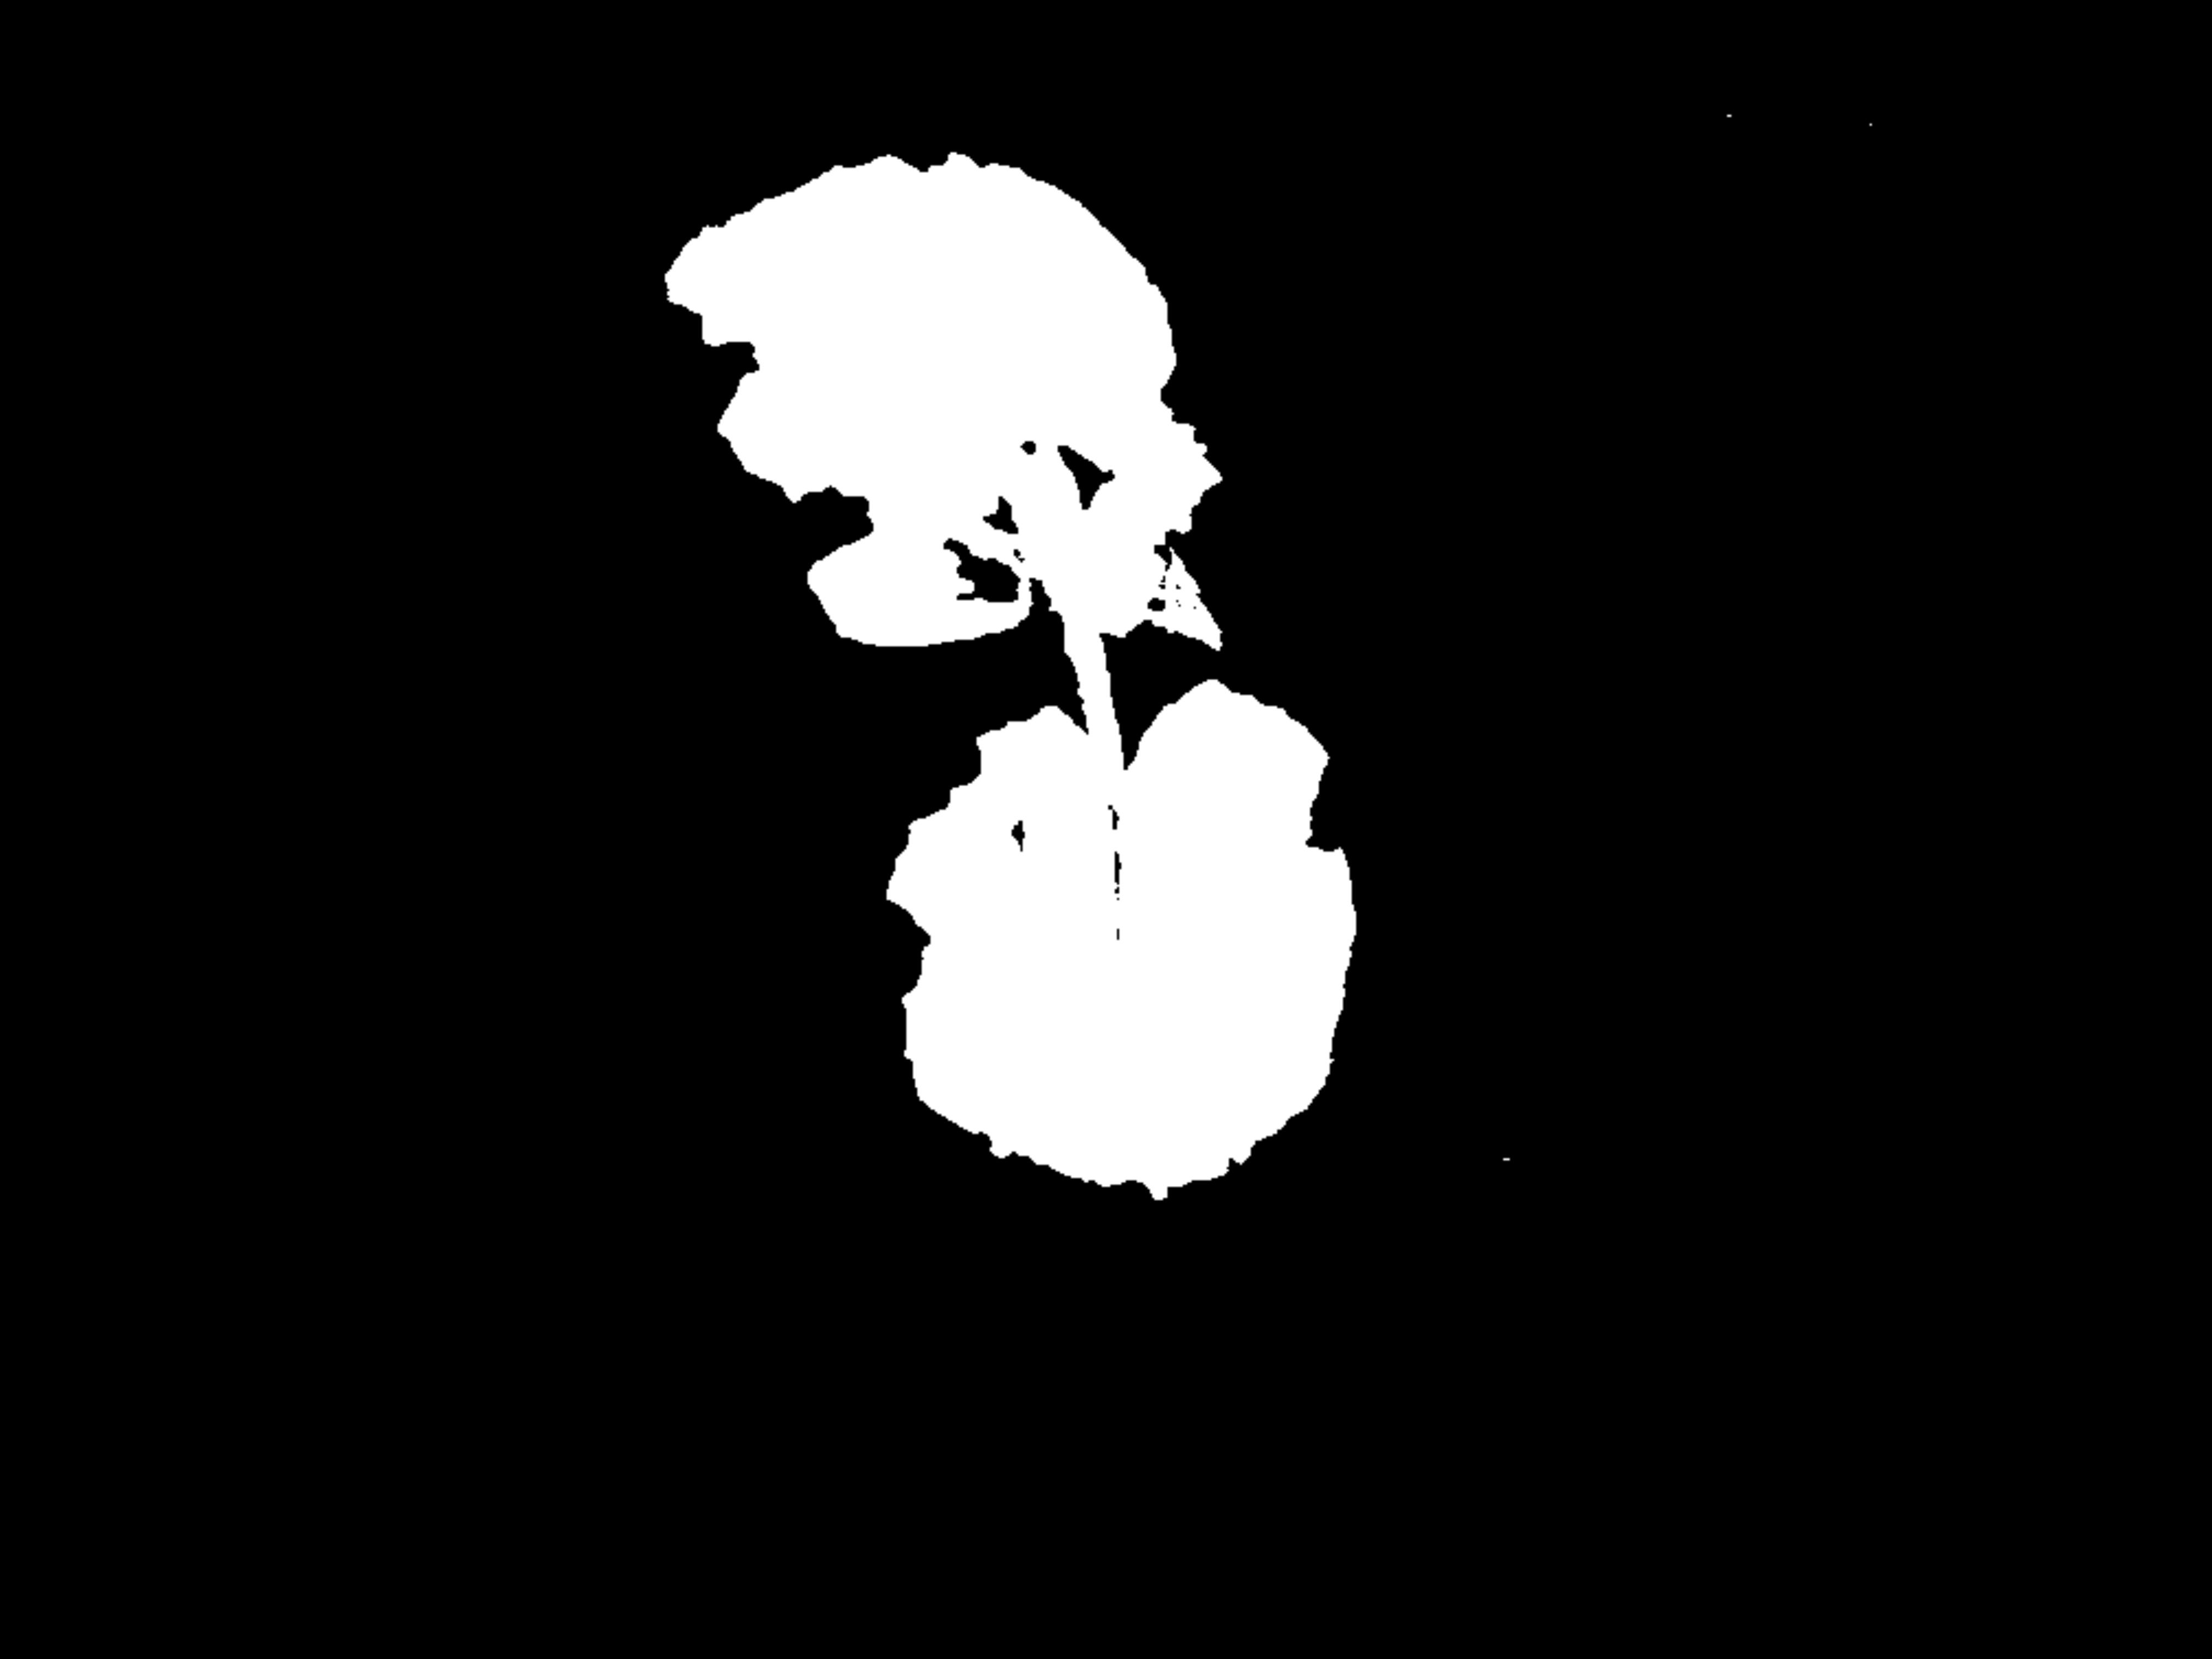
\includegraphics[width=.3\linewidth]{figures/IMG_1115-mask-unet.png}}
	\label{fig:unet-mask}
	\hfill
	\subfloat[Apply U-Net mask]{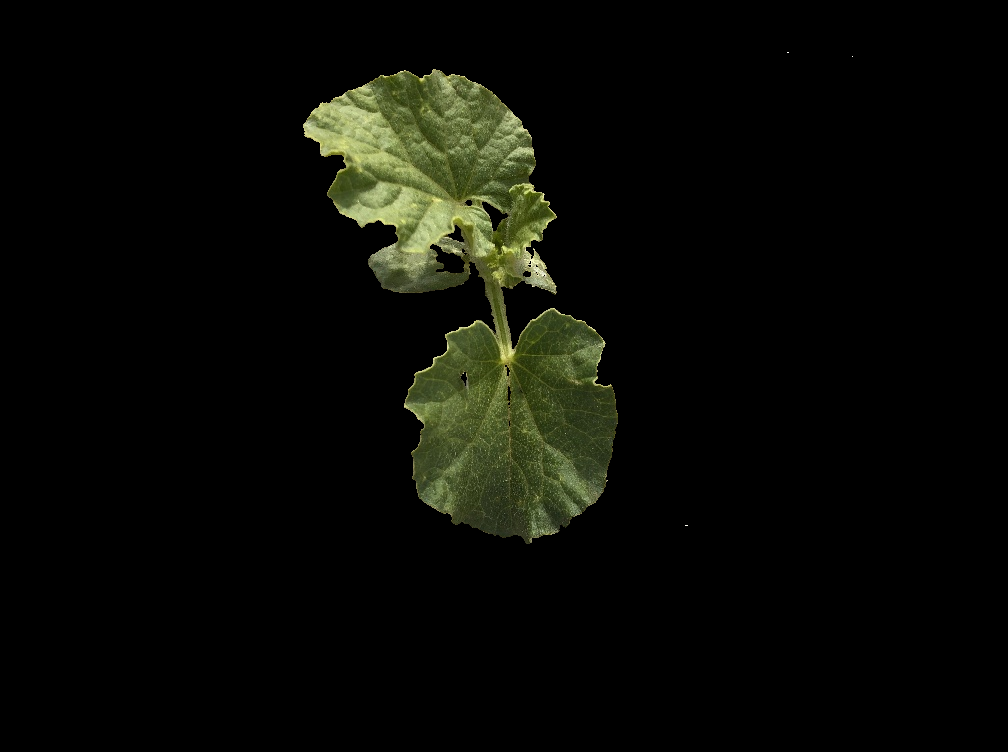
\includegraphics[width=.3\linewidth]{figures/IMG_1115-original-masked.png}}
	\label{fig:unet-original-masked}
	\caption[U-Net segmentation vs ground truth]{The mask produced with U-Net shows some errors within the leaf, but is quite close to a match for the ground truth.}
	\label{fig:u-net-segmentation}
\end{figure}


\section{Blob Identification}
Segmented images yield images with only vegetated pixels. Single items within those images are often called (somewhat generically) \textit{blobs}, and as that is the term generally used by the OpenCV software libraries used for image processing, that is the term adopted for this document. Blobs are the largest area of contiguous pixels with non-zero values.  The mask produced in the previous section is quite close to being suitable for the purposes of masking out non-vegetated pixels while allowing vegetated pixels of the original image, but requires some further refinement with morphological operations \textit{dilation} and \textit{closing} before it can be used, as the mask produced using only the index tends to hide portions of the vegetation.

\begin{figure}[h!]
	\centering
	\begin{subfigure}[h]{.48\textwidth}
	  \centering
	  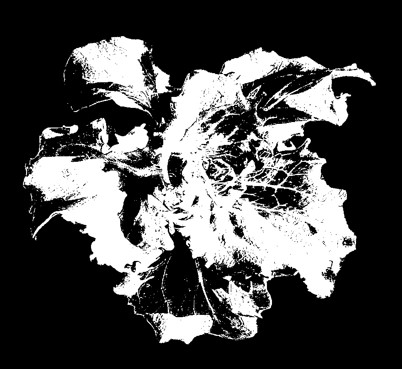
\includegraphics[height=5cm]{./figures/mask-raw.jpg}
	  \caption{Unrefined mask}
	  \label{fig:mask-raw}
	\end{subfigure}
	\hfill
	\begin{subfigure}[h]{.48\textwidth}
	  \centering
	  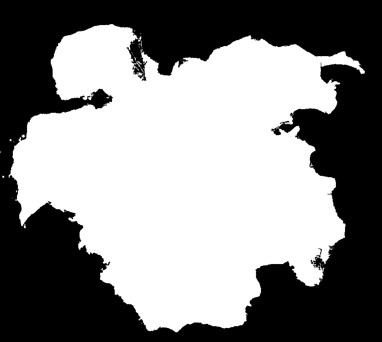
\includegraphics[height=5cm]{./figures/mask-processed.jpg}
	  \caption{Mask refined with pixel dilation and closing}
	  \label{fig:mask-processed}
	\end{subfigure}
	\caption[Mask before and after morphological refinements]{The unprocessed and refined mask. The unrefined mask in Figure~\ref{fig:mask-raw} would not allow for many of the details of the plant to be present in the final image. Note that large portions of some of the leaves are rendered as black, even as the vegetation edges are not. After the pixels are dilated with a 5x5 kernel of all 1s, the mask shown in Figure~\ref{fig:mask-processed} is produced, allowing all pixels within the leaf area to be present in the final image.}
	\label{fig:mask-before-and-after}
\end{figure}


Blobs are identified as an object requiring classification, but not yet classified. Figure~\ref{fig:original-masked} is an example of this concept. This image shows eight blobs that can be classified: three lettuce plants and a single weed plant that appears as five plants in the final image.

\section{Feature Extraction}
Once the vegetation is isolated and blobs identified, various features can be extracted for subsequent use in classification. These features include position-independent characteristics such as shape, hue, and textural characteristics as well as position-dependent features such as where a plant resides relative to the crop-line and size ratios between objects.  

\subsection{Shape Characteristics}
The shape of an object can be globally or locally described by various factors \parencite{Zhang2004-cm}. The problem quickly encountered in using shape in this instance is that a 3D object is projected on to a 2D plane, losing information in the process. The object in the resulting image is, of course, only a partial representation of the object as it exists in the real world. As section \ref{problem-overlap} shows in greater detail, even simple, but common occurrences such as object overlap complicate attempts to exploit shape. The classification examined in this paper will consider only the former, global descriptors that apply to an entire object. Shape parameters used in classification must exhibit three characteristics: scale invariance, rotation invariance, and translation invariance. Rotation invariance is, perhaps, the most relatable of these. While a camera mounted on a UAV or tractor will collect imagery in the same orientation, plants are not so obliging in their growth. Two plants might have leaves that may look extremely similar (and could be said to be of the same shape), but are rotated by 90\si{\degree}. Scale invariance is almost as easy to describe: two leaves have the same shape, but are simply of different size due to differences in the time of emergence. Translation invariance means that the same descriptor is derived without considering the position of the object within the image.  A fourth invariance is a bit more complex: viewpoint. While a camera capturing images as it passes overhead can always -- within a very small variation -- be considered to have the same viewpoint, the same does not hold true for the plants in the image. Two leaves can have the same physical shape, but differences in orientation with respect to the Z-axis (consider the case where the tip of one leaf is closer to the ground) produce significantly different descriptions of their shape. While a perfect shape descriptor would be invariant under all of these, it is typically not realistic to arrive at a shape descriptor that is invariant in all cases.
The shape parameters considered in this analysis are expressions describing the perimeter of the plant. The shape formulae used to extract the various shape features are given in Table~\ref{tab:shape-formulae}, but some concepts and formulae warrant further explanation.

\subsubsection{Shape Basics}
Before delving into some of the specifics of describing a shape, it may be necessary to discuss two topics that will appear is some of the details that follow: \textit{perimeter}, and \textit{major$/$minor axis}. The perimeter of an object, in this context, consists of the set of pixels that form the boundary of an object. An example perimeter is shown in \ref{fig:bounding-box}. The blue pixels following the edge of the plant defines the perimeter. While the perimeter is a concept that is probably most familiar to a wide audience, the major and minor axes are probably not. The major axis is the longest line that can be drawn through an object. If two objects of equal area are considered, one circular and one oval, the oval will have a longer major axis. The minor axis is considered to be the longest line that can be drawn perpendicular to the major axis.

\begin{figure}[h!]
	\centering
	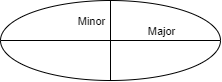
\includegraphics[scale=0.5]{./figures/shape-major-minor.png}
	\caption[Major/Minor Axis]{The major/minor axis of an object are illustrated by this simple example using an oval. The major axis is the longest line that can be drawn though the oval, and the minor axis is the longest line that can be drawn perpendicularly though that axis.}
	\label{fig:major-minor}
\end{figure}


\subsubsection{Bounding Box and Convex Hull}
An object can be said to have rectangular box of minimum size that completely encloses the object, commonly termed the \textit{bounding box}. The box placed around the object without regard for orientation -- that is, the placement makes no attempt to align the edges of the box with the edges of the image, so it may appear tilted at normal viewing angles. The \textit{convex hull}, likewise, is a convex shape with straight lines and of minimum size that completely encloses the object.   
\begin{figure}[h!]
	\centering
	\begin{subfigure}[h]{.48\textwidth}
	  \centering
	  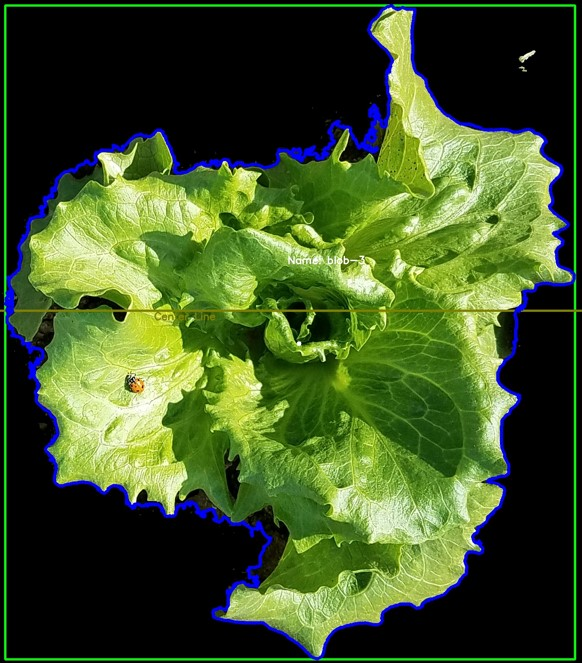
\includegraphics[height=5cm]{./figures/shape-bounding-box.jpg}
	  \caption{A bounding box}
	  \label{fig:bounding-box}
	\end{subfigure}
	\hfill
	\begin{subfigure}[h]{.48\textwidth}
	  \centering
	  \includegraphics[height=5cm]{./figures/shape-convex-hull.jpg}
	  \caption{A convex hull}
	  \label{fig:convex-hull}
	\end{subfigure}
	\caption[Bounding box and convex hull]{A bounding box and a convex hull (both noted in green) surround an object, but a convex hull is a shape with the minimum size that can contain the object. A bounding box is the minimum sized rectangle that can contain the object.}
	\label{fig:bounding-and-hull}
\end{figure}
The convex hull is a simple polygon whose vertices are a subset of the points found in the edge of the original shape. A widely used algorithm for determining the convex hull, \textit{Graham's Scan} is fairly efficient, $\mathcal{O}(n\log n)$, as \citeauthor{Klette2004-qz} show in this excerpt (altered for clarity with assistance from lecture notes from \citeauthor{Prosser1998-mi}). \parencite{Klette2004-qz}
\begin{quote}
\begin{enumerate}
	\item{Find the bottom-most point by comparing \textit{y} coordinate of all points. If there are two points with the same \textit{y} value, then the point with smaller \textit{x} coordinate value is considered. Let the bottom-most point be $P0$. Put $P0$ at first position in output hull.}
	\item{Sort the remaining points $p_i$ of $S$ in order of increasing angles $\eta_i$; if the angle is the same for more than one point, keep only the point furthest from $p$. Let the resulting sorted sequence of points be $q_i,..., q_m$.}
	\item{Initialize $C(S)$ by the edge between $p$ and $q_1$.}
	\item{Scan through the sorted sequence. At each left turn, add a new edge to $C(S)$; skip the point if there is no turn (a collinear situation); backtrack at each right turn.}
\end{enumerate}
\end{quote}
The most salient problem with the convex hull, however, is one that will have an adverse affect on all shape descriptors: distortions introduced by the resolution of the same object at different altitudes. That is, the edges are described by fewer pixels as the distance between the camera and plant increases, resulting in increased pixelation. While this can be minimized to some extent by blurring the image prior to performing the hull calculations, the hull is still distorted by this lower resolution.

\subsubsection{Area \& Size Ratio}
The area of the plant in the segmented image is simply the number of pixels with non-zero values. The term \textit{area} in this context is considered only in terms of pixels, not how much the pixel captures of the ground (e.g., the $cm^2$ each pixel represents). The relative area of two plants can then be compared to predict membership in a class. For instance, if a plant is $\frac{1}{3}$ the size of the largest plant in the image it is more likely than not a weed. This ratio is highly dependent on the development phase of the crop, as the reverse could be true for crop just emerging compared to much larger weeds. For the classification purposes presented here, the larger item is presumed to be crop.

% Figure produced with this command
% make weeds-no-db INPUT=/cygdrive/d/dissertation/ OUTPUT=/cygdrive/d/dissertation/output/ TRAINING=/cygdrive/d/maricopa-test/imbalance/processed/final/corrected.csv THRESHOLD=TRIANGLE INDEX=com2 DECORATIONS=area SESSION=shape
\begin{figure}[h!]
	\centering
	\includegraphics[height=4cm]{./figures/shape-area.jpg}
	\caption[Shape attribute: Area \& Size Ratio]{The area of the object in terms of numbers of pixels. By itself, this is not a particularly useful metric, but it may be useful to consider the relative sizes of plants to each other. As can be seen in this example, the crop plant is several times the size of the weed. This is, of course, highly dependent on the phase of development and how long the weed has been allowed to grow.}
	\label{fig:shape-area}
\end{figure}

\subsubsection{Length/Width Ratio}
\label{sec:length-width-ratio}
The ratio of width to length is not -- as the name might imply -- a simple ratio of two measurements, but is expressed as:
\begin{equation}
S = 
	\begin{bmatrix}
	Var(X) & Cov(XY) \\[0.3em]
	Cov(XY) & Var(Y) \\[0.3em]
	\end{bmatrix},
\lambda = \frac {eig_{1}(S)} {eig_{2}(S)}
\end{equation}
Where $eig_{1}(S)$ and $eig_{2}(S)$ are the maximum eigenvalues of the matrix $S$, with $\lambda$ representing the ratio. (\cite{Lin2017-xq}) The X and Y positions refer to an object's perimeter -- the boundary between an object's edge and the background.

% Figure produced with this command
%  make weeds-no-db INPUT=/cygdrive/d/dissertation/ OUTPUT=/cygdrive/d/dissertation/output/ TRAINING=/cygdrive/d/maricopa-test/imbalance/processed/final/corrected.csv THRESHOLD=TRIANGLE INDEX=com2 DECORATIONS=lw_ratio SESSION=shape

\begin{figure}[h!]
	\centering
	\includegraphics[height=4cm]{./figures/shape-lw-ratio.jpg}
	\caption[Shape attribute: Length-Width ratio]{The length-width ratio of plants. Note that the length-width ratio of the plant on the left of the image cannot be determined, as it is cut off, a common occurrence in images.}
	\label{fig:shape-area}
\end{figure}

\subsubsection{Boundary Descriptors}
Once again focusing on the edge of an object there are two global descriptors of an object's edge that are used here: the bending energy and the radial distance. Describing the bending energy of an object involves a few preliminary steps. Changes in the $(x,y)$ position of edge pixels can be described by a \textit{chain code}. A chain code representation of a boundary describes unit length changes in the $(x,y)$ positions of the boundary,  where changes in the position are noted by their position in a matrix:

 \begin{figure}[h!]
	\centering
	\begin{subfigure}[h]{.4\textwidth}
	  \centering
	  \includegraphics[height=3cm]{./figures/chain-code-matrix.jpg}
	  \caption{Chain code matrix}
	  \label{fig:chain-code-matrix}
	\end{subfigure}
	%\hfill
	\begin{subfigure}[h]{.4\textwidth}
	  \centering
	  \includegraphics[height=3cm]{./figures/chain-code-cells.jpg}
	  \caption{Example edge}
	  \label{fig:chain-example}
	\end{subfigure}
%	\hfill
%		\begin{subfigure}[h]{.25\textwidth}
%	  \centering
%	  \includegraphics[height=2cm]{./figures/chain-code-result.jpg}
%	  \caption{Result}
%	  \label{fig:chain-result}
%	\end{subfigure}
	\caption[Boundary chain codes]{Chain codes of the transitions of an object's edge -- as seen in successive pairs of coordinates -- are described by positions within an 8 position matrix, with each position noting the change in the $(X, Y)$ coordinate (steps of length 1 along the $x,y$ axis lines and of length $\sqrt{2}$ for diagonal movements). In this example the edge has a chain code of 2,1,0,7,7,0,1,1. While this example shows an open curve with a distinct beginning and ending, the boundary of a plant is a closed curve with no distinct end or beginning. A 4 direction matrix is is also used, as is a general $N$-directional chain $(N > 8\ and\ N =2^k)$, although those variants are not addressed in this document. The 8 position matrix is, perhaps, the most relatable, as changes in adjacent boundary pixels always take one of the 8 possibilities present in the matrix. The matrix shown in \ref{fig:chain-code-matrix} is a $3x3$ matrix, but the middle position (implying no change) is not possible -- this is simply an illustration.}
	\label{fig:chain-codes}
\end{figure}

The \textit{$\kappa$-slope} of a given boundary point $(X_i, Y_i)$ is estimated from the slope of the line joining positions $(X_{i-k/2}, Y_{i-k/2})$ and $(X_{i+k/2}, Y_{i+k/2})$ with this equation:
\begin{equation}
\tan^{-1}\left(\frac{Y_{i+k/2} - Y_{i-k/2}}{X_{i+k/2} - X_{i-k/2}}\right)
\end{equation}
 
 The \textit{$\kappa$-curvature} of the boundary at location $(X_i,Y_i)$ can be estimated by this equation:
 \begin{equation}
 \tan^{-1}\left(\frac{Y_{i+k} - Y_{i}}{X_{i+k} - X_{i}}\right) - \tan^{-1}\left(\frac{Y_{i} - Y_{i-k}}{X_{i} - X_{i-k} }\right)
 \end{equation}
 The goal of this metric is to assess the concavity or convexity of points along the perimeter. Consider the weed in Figure \ref{fig:curvature-weed} with the computed $\kappa$-curvature.
 
  \begin{figure}[h!]
	\centering
	\begin{subfigure}[h]{.4\textwidth}
	  \centering
	  \includegraphics[height=4cm]{./figures/for-curvature-blob-1.jpg}
	  \caption{Weed}
	  \label{fig:curvature-weed}
	\end{subfigure}
	%\hfill
	\begin{subfigure}[h]{.4\textwidth}
	  \centering
	  \includegraphics[height=4cm]{./figures/curvature-blob-1.jpg}
	  \caption{$\kappa$-curvature}
	  \label{fig:curvature-plot}
	\end{subfigure}
	\caption[Example of $\kappa$-curvature]{The $\kappa$-curvature of various points around the perimeter of the weed are illustrated here. Positive values are indicative of convex shapes. Likewise, negative values indicate concave shapes.  While it is tempting to relate the values shown in the graph to the image displayed (as the figure invites the user to do), exact correlation is not advised, as the points sampled may not match the finer details that can be seen in the leaf. This example uses a relatively coarse sampling. However, the image does show a pronounced curve at the lower edge that can be seen in the curvature plot.}
	\label{fig:curvature}
\end{figure}
This leads to a global descriptor used in classification: \textit{bending energy}. Bending energy is typically described as the energy required to bend a rod to the shape under consideration, and is expressed as the sum of squares of the $\kappa$-curvature over the boundary length $L$.
\begin{equation}
\frac{1}{L} \sum_{p=1}^{L}\kappa(p)^2
\end{equation}
While there will be no bending of rods required for classification, this global metric can be used to express the overall shape of the perimeter, exploiting the fact that weeds in a crop and the crop itself exhibit different shapes.

% Figure produced with this command
%  make weeds-no-db INPUT=/cygdrive/d/dissertation/ OUTPUT=/cygdrive/d/dissertation/output/ TRAINING=/cygdrive/d/maricopa-test/imbalance/processed/final/corrected.csv THRESHOLD=TRIANGLE INDEX=com2 DECORATIONS=bending SESSION=shape

\begin{figure}[h!]
	\centering
	\includegraphics[height=4cm]{./figures/shape-bending.jpg}
	\caption[Shape attribute: Bending Energy]{The bending energy}
	\label{fig:shape-bending}
\end{figure}

The \textit{radial distance} can also be used to describe the shape. \citeauthor{Kilday1993-aq}, in a study of classification of lesions in mammogram images, describe techniques to exploit the radial distance of a shape \parencite{Kilday1993-aq}. Before stepping through those techniques, it may prove useful to step back a bit and look at radial distances of an object.
\begin{figure}[H]
	\centering
	\includegraphics[width=.25\linewidth]{./figures/radial-distance.jpg}
	\caption[Radial distance from object centroid]{The radial distance from object centroid is noted by \textit{d} in this figure. Scale invariance is achieved by expressing functions of the normalized distance (using the maximum radial distance of the object).}
	\label{fig:radial-distance}	
\end{figure}
As Figure \ref{fig:radial-distance} shows, the radial distance referred to is the distance from an object's centroid (geometric center) to its perimeter $(x,y)$ locations. To make this distance scale invariant, the normalized distance to the maximal distance is used. Using the normalized radial distance, the mean and standard deviation is given by these equations for the $i^{th}$ blob:
\begin{equation}%\labeleqn{Radial distance mean and standard deviation}
\bar{x}_i = \frac{1}{N}\sum_{k=1}^{N}r_k \qquad
\sigma_i = \sqrt{\frac{1}{N}\sum_{k=1}^{N}({r_k} - \bar{x}_i)^2}
\end{equation}
By themselves these metrics may not be particularly useful in predicting class membership, however these provide useful information for metrics that may be. The number of times the normalized radial distance crosses the mean, for instance, provides an estimate of the roughness of a perimeter. So while the radial distance is not used directly, it is used indirectly as a roughness metric.


% Begin table of shape equations
\begin{longtable}{x{\dimexpr.15\columnwidth-2\tabcolsep}
                  x{\dimexpr.425\columnwidth-2\tabcolsep}
                  x{\dimexpr.425\columnwidth-2\tabcolsep}}
%\begin{hyphenrules}{nohyphenation}
    \caption{Shape Features}\label{tab:shape-formulae}  \\
\toprule
{\textbf{Feature}} & {\textbf{Formula}} & {\textbf{Comment}}
\tabularnewline
\midrule
    \endfirsthead
%%%%
    \caption{Shape Features (cont.)}\label{tab:shape-formulae}  \\
\toprule
{\textbf{Feature}} & {\textbf{Formula}} & {\textbf{Comment}}
\tabularnewline
\midrule
    \endhead
%%%%
\midrule[\heavyrulewidth]
\multicolumn{3}{r}{\footnotesize\itshape
                   Continued on the next page}
    \endfoot
%%%%
\bottomrule
    \endlastfoot
%%%%
		Perimeter
		& \begin{minipage}[t]{0.3\textwidth}
			$\sum_{i=1} ^{N-1}\left|X_1 - X_{i+1}\right| $
		   \end{minipage}     
		& Count of pixels forming the boundary of an object
\tabularnewline\addlinespace

		Major/Minor Axis     
		& $\sqrt{(x_2 - x_1)^2 + (y_2 - y_1)^2} $                    
		& Major axis is the longest line that can be drawn through the object. Minor axis is the longest line that can be drawn through the object such that the line remains perpindicular to the major axis.
\tabularnewline\addlinespace

		Compactness      
		& \begin{minipage}[t]{0.3\textwidth}
			$\frac{4\pi * area}{(perimeter)^2}$ 
		   \end{minipage}
		& Ratio of an object's area to the area of a circle having the same perimeter 
\tabularnewline\addlinespace

		Elongation      
		& $\frac{width_{bounding}}{length_{bounding}}$ 
		& Ratio of the width of the object's bounding box to its width
\tabularnewline\addlinespace

		Eccentricity      
		& $\frac{length_{minor}}{length_{major}}$
		& Ratio of the minor to major axis
\tabularnewline\addlinespace

		Convexity   
		& $\frac{convex~perimeter}{perimeter}$ 
		& Ratio of the convex perimeter to the perimeter.
\tabularnewline\addlinespace

		Solidity    
		& $\frac{area}{convex~area}$ 
		&  Ratio of an object's area to its convex area. 
\tabularnewline\addlinespace

		Circularity    
		& $\frac{4\pi * area}{convex~perimeter}$ 
		& Ratio of an object's area to its convex perimeter. 
\tabularnewline\addlinespace


		Shape Index    
		& $\alpha = \frac {e} {4 \sqrt{A}}$ 
		&  Relationship between an object's perimeter and its area
\tabularnewline\addlinespace

		Width/Length Ratio
		& \begin{minipage}[h]{0.10\textwidth}
			\begin{eqnarray*}
				S = 
				\begin{bmatrix}
					Var(X) & Cov(XY) \\[0.10em]
					Cov(XY) & Var(Y) \\[0.10em]
				\end{bmatrix}
			\lambda = \frac {eig_{1}(S)} {eig_{2}(S)}
			\end{eqnarray*}
		  \end{minipage}
		& See section~\ref{sec:width-length-ratio}
\tabularnewline\addlinespace

		Bending Energy    
		& $\frac{1}{L} \sum_{p=1}^{L}\kappa(p)^2$ 
		&  The energy required to bend a rod to the perimeter shape
\tabularnewline\addlinespace

\label{table:shape-formulae}
\end{longtable}
}

% End table of shape equations

%
% C O L O R
%
\subsection{Color}
Color presentations of an image are ubiquitous, and while the Red-Blue-Green (RGB) color space is widely familiar, an image can be represented in other color spaces. RGB representation is nothing more than three channels, each of which note (respectively) the levels of Red, Green, and Blue in the image.  Examining each of these channels in isolation usually results in an odd -- but fairly realistic -- view of an object. Other color spaces do not alter the image itself, just the representation of the colors found in the image.  Choosing to represent the amounts of red, green, and blue in an image is just as arbitrary as other mechanisms, however closely aligned it is with human color perception. Other schemes provide somewhat equivalent -- but typically superior -- encodings of the colors found in the image. The representations are, most often, superior in some way, perhaps either in the range of colors represented or the efficiency of that representation. Each of the representations may have an advantage over the RGB model, but those advantages are of no concern here. Classification will use both components of those representations (i.e., the mean of an object's \textit{hue} in the HSI space) as well as the data contained within those components being used in other techniques (GLCM, for instance). All of the color representation schemes that follow all follow the RGB model in one key respect: each represents an image using three channels. RGB represents the amount of green in the image in the G channel, while the HSV space represents the saturation of the hue in the S channel. This characteristic is not something that will be exploited in classification, however. The representation itself may be superior in some aspect to other representations, but aspects of that representation that can be used for classification is the concern in this problem space. While viewing the vegetation in one of the components can be fairly seen as not accurately representing the same experience one would have in viewing the object in daylight or other presentations, these components often have information relevant to the task at hand. This section presents a brief overview of the color spaces used in classification.

\subsubsection{RGB}
The RGB color space is both the most frequently encountered and easily explained colorspace. The levels or red, green, and blue are expressed as the amount of these colors for each pixel. The normal human eye contains three types of color-sensitive cone cells. Each cell is responsive to light of either longer or shorter wavelengths, which we often refer to as red, green, and blue. A triple (r,g,b) is used to describe the color values of a pixel ranging from completely black, (0, 0, 0), to completely white (255, 255, 255).

%
% Figure from here:
% https://en.wikipedia.org/wiki/RGB_color_spaces
%
\begin{figure}[H]
	\centering
	\includegraphics[width=5cm]{./figures/RGB_Cube_Show_lowgamma_cutout_b.png}
	\caption[RGB Cube]{RGB Cube. (Creative Commons)}
	\label{fig:rgb-cube}
\end{figure}

Consider the color values encountered for both a weed and a crop. Figure \ref{fig:transects-rgb} illustrates the values encountered for both the ground and vegetation, but notice that the ground beside the weed exhibits significant overlap with the value encountered with values shown for the crop.  The RGB values might be of interest to examine, but are probably not something that can be exploited directly for classification. This is, however, a fine illustration of a concept that will be exploited: weeds and crop have different color content, even if that difference is not apparent.  The crop, for instance, has a noticeably lower red content that the weed exhibits.
% Figure generated with
% make plot-for-document X=1236 Y=1160 X2=1567 Y2=1141 SUBJECT=Weed BAND=rgb INPUT=/cygdrive/d/dissertation/20190118_124250.jpg  COLOR=rgb
% Change the SUBJECT to reflect the X,Y coordinates, as each figure requires two plots -- the two coordinates are just for the image
% python plot.py -x 1236 -y 1160 -x2 1567 -y2 1141 -i `cygpath -w /cygdrive/d/dissertation/20190118_124250.jpg` -s Weed -l logging.ini -c rgb -b 0 -b 1 -b 2 -t band --length 100
% This generates two files: transect-image.jpg and transect-plot.png -- rename the latter 

\begin{figure*}[h]
	\centering
	\subfloat[Original\centering]{\includegraphics[width=4cm]{./figures/transect-image.jpg}\label{fig:transect-original-rgb}}
	\hfill
	\subfloat[Weed\centering]{\includegraphics[width=6cm]{./figures/transect-plot-rgb-weed.png}\label{fig:transect-weed-rgb}}
	\hfill
	\subfloat[Crop\centering]{\includegraphics[width=6cm]{./figures/transect-plot-rgb-crop.png}\label{fig:transect-crop-rgb}}
	\caption[RGB Transects]{Transects of vegetation in the RGB color space. Figure \ref{fig:transect-original-rgb} shows the transect locations for the weed (\ref{fig:transect-weed-rgb}) and crop (\ref{fig:transect-crop-rgb}) Note the distinct change of the transect as it passes through the weed, where ground pixels are captured. Both of the transects capture a portion of the ground to the left of each plant.}
	\label{fig:transects-rgb}
\end{figure*}
	
\subsubsection{Hue-Centric colorspaces: HSI \& HSV}
The terms {\it color} and {\it hue} are often used interchangeably, and while this is mostly true, hue refers to the dominant color family. Black and white are colors, for instance, but they are almost never referred to as a hue. In this case, the image is converted to the Hue, Saturation, and Value ({\it HSV}) colorspace and the mean value for the hue of a blob's pixels is taken. The saturation of a color expressed by a component of the Hue, Saturation, and Intensity ({\it HSI}) colorspace and the mean value for the saturation of a blob's pixels is taken. (\cite{Forsyth2012-hy})

The Hue, Saturation, and Intensity (HSI) and the Hue, Saturation, and Value (HSV) color spaces are cylindrical-coordinate representations of the RGB color model.  These models, first developed in the 1970s, rearrange the RGB cube representation to be more perceptually relevant. Both models are closely related in that they share an common expression of hue and saturation. While it is a bit simplistic to state, and as the similarities in the name imply, the values for \textit{hue} and \textit{saturation} are identical for these two colorspaces, leaving focus on the \textit{intensity} and \textit{value} components as the unique values that will be analyzed. \parencite[p.~84]{Forsyth2012-hy} Somewhat confusingly, HSV is sometimes referred to as HSB (or Hue, Saturation, and Brightness); likewise, HSI is  is sometimes referred to as HSL (Hue, Saturation, and Lightness), but the two are identical for the most part. In this cylindrical representation, hue is expressed as the angular dimension, red (at 0\si{\degree}), passing through green (at 120\si{\degree}) and blue (at 240\si{\degree}) In each representation, the vertical axis comprises the neutral, achromatic, or gray colors ranging, from top to bottom, white at lightness 1 (value 1) to black at lightness 0 (value 0).

\begin{figure}[H]
	\centering
	\begin{subfigure}[h]{.45\textwidth}
		\centering
		\includegraphics[width=6cm]{./figures/HSV_color_solid_cylinder_saturation_gray.png}
		\caption{HSV/HSB Cylinder}
		\label{fig:hsv}
	\end{subfigure}
	\hfill
	\begin{subfigure}[h]{.45\textwidth}
		\centering
		\includegraphics[width=6cm]{./figures/HSL_color_solid_cylinder_saturation_gray.png}
		\caption{HSL/HSI Cylinder}
		\label{fig:hsl}
	\end{subfigure}
	\caption[HSL and HSV color representations]{HSL and HSV color representations. (Creative Commons)}
	\label{fig:overlap}
\end{figure}

\begin{figure*}[h]
	\centering
	\subfloat[Original\centering]{\includegraphics[width=4cm]{./figures/transect-image.jpg}\label{fig:transect-original-rgb}}
	\hfill
	\subfloat[Weed\centering]{\includegraphics[width=6cm]{./figures/transect-plot-hsv-weed.png}\label{fig:transect-weed-hsv}}
	\hfill
	\subfloat[Crop\centering]{\includegraphics[width=6cm]{./figures/transect-plot-hsv-crop.png}\label{fig:transect-crop-hsv}}
	\caption[HSV Transects]{Transects of vegetation in the HSV color space. Figure \ref{fig:transect-original-rgb} shows the transect locations for the weed (\ref{fig:transect-weed-hsv}) and crop (\ref{fig:transect-crop-hsv}) Note the distinct change of the transect as it passes through the weed, where ground pixels are captured. Both of the transects capture a portion of the ground to the left of each plant.}
	\label{fig:transects-hsv}
\end{figure*}

\begin{figure*}[h]
	\centering
	\subfloat[Original\centering]{\includegraphics[width=4cm]{./figures/transect-image.jpg}\label{fig:transect-original-rgb}}
	\hfill
	\subfloat[Weed\centering]{\includegraphics[width=6cm]{./figures/transect-plot-hsi-weed.png}\label{fig:transect-weed-hsi}}
	\hfill
	\subfloat[Crop\centering]{\includegraphics[width=6cm]{./figures/transect-plot-hsi-crop.png}\label{fig:transect-crop-hsi}}
	\caption[HSI Transects]{Transects of vegetation in the HSI color space. Figure \ref{fig:transect-original-rgb} shows the transect locations for the weed (\ref{fig:transect-weed-hsi}) and crop (\ref{fig:transect-crop-hsi}) Note the distinct change of the transect as it passes through the weed, where ground pixels are captured. Both of the transects capture a portion of the ground to the left of each plant.}
	\label{fig:transects-hsv}
\end{figure*}


\subsubsection{YIQ}
The YIQ model (lacking a friendlier name, it simply goes by the initials of its constituent channels) of color was used by the (analog) NTSC color TV system. Later, digital transmission schemes used different color spaces, notably the YCbCr that will be addressed in more detail in a separate section. These schemes have a common approach: \textit{chrominance} (a color component) is added to a black and white image. In the YIQ model, $Y$ represents the luma information (black and white), with $I$ (in-phase) representing red-cyan contrast, and $Q$ (quadature) representing magenta-green contrast) the chrominance information.  The YIQ and YUV color spaces are variants of each other, as they follow the same basic representation, a luma representation with chrominance in two additional channels.  The U \& V values can be considered the X \& Y axes within the color space, while $I$ \& $Q$ are a second set of axes rotated by $33^o$. Different (and now obsolete) technologies used these encodings: YUV was used by PAL, and YIQ was used by NTSC.


The processing employed here is to convert the image to the YIQ color space and take the mean value for the $I$, or in-phase component for the blob's pixels. (\cite{MathWorks_undated-jg})
\begin{figure}[h!]
	\centering
	\includegraphics[scale=0.4]{./figures/yiq.png}
	\caption[YIQ color space at $Y = 0.5$]{A view of the YIQ color space for $Y=0.5$. Of special note here is that the $I$ and $Q$ axes are normalized from -1 to +1. In the YIQ space, the $Y$ component is used by black and white receivers (perhaps difficult to find nowadays), as it represents the Luma information. (Creative Commons)}
	\label{fig:yiq-space}
\end{figure}
The $I$ component is the feature of interest here, and conversion of RGB to YIQ is achieved with this transformation:
\begin{equation}
	\begin{bmatrix}
	Y \\[0.3em]
	I \\[0.3em]
	Q \\[0.3em]
	\end{bmatrix}
	\approx
	\begin{bmatrix}
	0.299 & 0.587 & 0.114 \\[0.3em]
	0.5959 & -0.2746 & -0.3213\\[0.3em]
	0.2115 & -0.5227 & 0.3112 \\[0.3em]
	\end{bmatrix}
	\begin{bmatrix}
	R \\[0.3em]
	G \\[0.3em]
	B \\[0.3em]
	\end{bmatrix}	
\end{equation}
Here we also see convenience and ubiquity of the RGB colorspace. More often than not, color spaces are expressed as transformation from the RGB values, a technique that will be used in this section.

As Figure \ref{fig:hue_vs_inphase} shows, the tight grouping of the mean hue of an object class (it is not particularly important, at this juncture, what class $0$ and $1$ actually are), while interesting, is not something that can be used to predict if a plant is a weed or crop.  The somewhat greater variation of the other class is, likewise, interesting, but not an aspect of the data that can be exploited in classification. The in-phase component of the YIQ space, however, demonstrates a fairly clean separation that can, as there is little overlap between the two classes.


\begin{figure}[H]
	\begin{subfigure}[h]{0.48\linewidth}
		\includegraphics[width=1\linewidth]{./figures/hsi-hue.jpg}
		\caption{Hue in HSI}
		\label{subfig:hue}	
	\end{subfigure}
	\hfill
	\begin{subfigure}[h]{0.48\linewidth}
		\includegraphics[width=1\linewidth]{./figures/yiq-in-phase.jpg}
		\caption{In-phase in YIQ}
		\label{subfig:in_phase}		
	\end{subfigure}%
	\caption[Prediction using hue in HSI and In-phase in YIQ]{While the grouping of hue values is certainly tighter in one group (Figure~\ref{subfig:hue}), the complete overlap between means that group assignments cannot be made with confidence. In contrast, the values of the in-phase component in the YIQ space (Figure~\ref{subfig:in_phase}) shows relatively clean separation between the two groups.}
	\label{fig:hue_vs_inphase}
\end{figure}

\begin{figure*}[h]
	\centering
	\subfloat[Original\centering]{\includegraphics[width=4cm]{./figures/transect-image.jpg}\label{fig:transect-original-rgb}}
	\hfill
	\subfloat[Weed\centering]{\includegraphics[width=6cm]{./figures/transect-plot-yiq-weed.png}\label{fig:transect-weed-yiq}}
	\hfill
	\subfloat[Crop\centering]{\includegraphics[width=6cm]{./figures/transect-plot-yiq-crop.png}\label{fig:transect-crop-yiq}}
	\caption[YIQ Transects]{Transects of vegetation in the YIQ color space. Figure \ref{fig:transect-original-rgb} shows the transect locations for the weed (\ref{fig:transect-weed-rgb}) and crop (\ref{fig:transect-crop-rgb}) Note the distinct change of the Luma line of the transect as it passes through the weed into the area where ground pixels are captured, but the Blue-difference and Red-Difference values remain relatively stable. Contrast this with what is shown in the transect of the crop, where the same sort of abrupt change is seen in the Luma, but the difference between the Blue-difference and Red-difference is more noticeable. Both of the transects capture a portion of the ground to the left of each plant.}
	\label{fig:transects-yiq}
\end{figure*}


\subsubsection{CIElab}
Often going by the somewhat awkward acronym L*a*b*, this colorspace was intended to approximate human vision, as the $L$ component expresses  the lightness of an object, an attribute seen a more applicable to perception of an object's color than the RGB model of mixtures of the three underlying colors.  The $A$ and $B$ components contain data about green to red, and blue to yellow, respectively, the four unique colors humans can perceive. While the space is not completely uniform, it is often employed in describing small changes in color. That is, numeric changes correspond to perceptual changes. The CIElab color space was standardized in the mid-1970s but remains in widespread use today. \parencite{Wikipedia_contributors2023-xt}  The $A$ and $B$ axes are theoretically unbound, but are typically limited to some practical range, say +127 to -127. 

\begin{figure}[H]
	\centering
	\includegraphics[width=.35\linewidth]{./figures/cielab-colorspace.jpg}
	\caption[CIElab colorspace]{In the CIElab colorspace, positive values for $B$ indicate more yellow; likewise negative values for $B$ indicate more blue. The values for $A$ similarly indicate more red (positive) or more green (negative). This is often referred to as an \textit{opponent representation} (yellow-blue and red-green) (Illustration reproduced from Color Application Specialists)}
	\label{fig:cielab}	
\end{figure}

Perceptual uniformity and pragmatic implementation details aside, the use of this colorspace is motivated by some of its salient features, most notably the ability to capture small color changes. These small color changes are expected to be significant in distinguishing crop from weed.

\begin{figure*}[h]
	\centering
	\subfloat[Original\centering]{\includegraphics[width=4cm]{./figures/transect-image.jpg}\label{fig:transect-original-rgb}}
	\hfill
	\subfloat[Weed\centering]{\includegraphics[width=6cm]{./figures/transect-plot-cielab-weed.png}\label{fig:transect-weed-cielab}}
	\hfill
	\subfloat[Crop\centering]{\includegraphics[width=6cm]{./figures/transect-plot-cielab-crop.png}\label{fig:transect-crop-cielab}}
	\caption[CIELab Transects]{Transects of vegetation in the CIELab color space. Figure \ref{fig:transect-original-rgb} shows the transect locations for the weed (\ref{fig:transect-weed-rgb}) and crop (\ref{fig:transect-crop-rgb}) Note the distinct change of the Luma line of the transect as it passes through the weed into the area where ground pixels are captured, but the Blue-difference and Red-Difference values remain relatively stable. Contrast this with what is shown in the transect of the crop, where the same sort of abrupt change is seen in the Luma, but the difference between the Blue-difference and Red-difference is more noticeable. Both of the transects capture a portion of the ground to the left of each plant.}
	\label{fig:transects-cielab}
\end{figure*}

\subsubsection{YCbCr}
Often encountered for digital video, YCbCr encodes both luminance information ($Y$, black and white) and chrominance information ($Cb$, $Cr$). In that respect, of course, it is similar to other spaces separating luma from color encoding (YIQ, for instance). By separating the component the human eye is most sensitive to, brightness ($Y$) from color ($Cb$ and $Cr$), the color components can be altered to achieve efficiencies in storage or transmissions that would not be possible where each and every pixel must be represented by the levels of Red, Green, and Blue.  The $Cb$ and $Cr$ components represent the difference between a reference value and the blue or red component, respectively. The JPEG image format exploits these efficiencies in creating compressed images. While the efficiencies of the representation are not of interest in classification, the color representation is. This color space is similar to another encoding commonly encountered in digital video, YUV. The two spaces are nearly identical; YCbCr is a scaled version of YUV (used in analog broadcasts). This color space is also referred to by the somewhat shortened abbreviation YCC, although this document will continue to use YCbCr.

The ECMA report on the JPG file format gives this transformation for RGB to YCbCr:
\nocite{Ecma2019-yo}
\begin{equation}
	\begin{bmatrix}
	Y \\[0.3em]
	C_b \\[0.3em]
	C_r \\[0.3em]
	\end{bmatrix}
	\approx
	\begin{bmatrix}
	0.2126 & 0.7152 & 0.0722 \\[0.3em]
	-0.1146 & -0.3854 & 0.5 \\[0.3em]
	0.5 & -04542. & -0.458 \\[0.3em]
	\end{bmatrix}
	\begin{bmatrix}
	R \\[0.3em]
	G \\[0.3em]
	B \\[0.3em]
	\end{bmatrix}	
\end{equation}

\begin{figure*}[h]
	\centering
	\subfloat[Original\centering]{\includegraphics[width=4cm]{./figures/transect-image.jpg}\label{fig:transect-original-rgb}}
	\hfill
	\subfloat[Weed\centering]{\includegraphics[width=6cm]{./figures/transect-plot-ycbcr-weed.png}\label{fig:transect-weed-ycbcr}}
	\hfill
	\subfloat[Crop\centering]{\includegraphics[width=6cm]{./figures/transect-plot-ycbcr-crop.png}\label{fig:transect-crop-ycbcr}}
	\caption[YCbCr Transects]{Transects of vegetation in the YCbCr color space. Figure \ref{fig:transect-original-rgb} shows the transect locations for the weed (\ref{fig:transect-weed-rgb}) and crop (\ref{fig:transect-crop-rgb}) Note the distinct change of the Luma line of the transect as it passes through the weed into the area where ground pixels are captured, but the Blue-difference and Red-Difference values remain relatively stable. Contrast this with what is shown in the transect of the crop, where the same sort of abrupt change is seen in the Luma, but the difference between the Blue-difference and Red-difference is more noticeable. Both of the transects capture a portion of the ground to the left of each plant.}
	\label{fig:transects-ycbcr}
\end{figure*}


\subsection{Textural}
Textural descriptors of a object are formal expressions of the relationship pixel values have with one another, reducing a tactile experience to a numerical one. Common texture descriptions, bumpy, rough, smooth, etc., refer to a quality that is useful for a human description, but tends not to be particularly exact. Each of these descriptors, however, has a few attributes in common that can then be used to quantify them relative to a fingertip: the difference between high and low points, and the spacing of these high and low points. A smooth surface could be said to have low difference between high and low points, with small spacing. A rough surface would exhibit fairly large differences between high and low points with relatively wide spacing (at least compared to a human fingertip). While this list of descriptors is not comprehensive, and the additional quantification incomplete, this gives a sense of what is meant by a more formal texture description. Textural descriptors quantify (at least) two items: the neighborhood where a change is seen, and the direction of that change. Consider, for instance, the coat of a smooth-haired dog. Most of the hairs encountered would be aligned in the same direction, and in that direction the same texture would be encountered.
Classifying the texture is -- like color -- an analysis of the interior of the plant, and for this analysis three techniques will be used:  \textit{Grey-level Co-occurrence Matrix} (GLCM), \textit{Local Binary Pattern} (LBP) and \textit{Histogram of Oriented Gradients} (HOG). These approaches consider a pixel's relationship with surrounding pixels. 

\subsubsection{GLCM}
In \textit{Grey-level Co-occurrence Matrix} (GLCM) (\cite{Haralick1973-gr}, \cite{Hall-Beyer2017-nx}), Haralick describes the analysis of an image that has been converted to greyscale values to note the relationship. Before delving into the details of the use of GLCM, it might be helpful to address what it is.

\begin{figure}[H]
	\begin{subfigure}[h]{0.28\linewidth}
		\includegraphics[height=3cm]{./figures/glcm-example.jpg}
		\caption{Sample image}
		\label{subfig:glcm_sample}	
	\end{subfigure}
	\hfill
	\begin{subfigure}[h]{0.28\linewidth}
		\includegraphics[height=3cm]{./figures/glcm-numeric.jpg}
		\caption{Numeric equivalent}
		\label{subfig:glcm_numeric}		
	\end{subfigure}
	\hfill
	\begin{subfigure}[h]{0.28\linewidth}
		\includegraphics[height=3cm]{./figures/glcm-matrix.jpg}
		\caption{Co-occurence matrix}
		\label{subfig:glcm_matrix}		
	\end{subfigure}%
	\hfill
	\caption[GLCM matrix explained]{The GLCM matrix concept is based on the contents of adjacent pixels. \ref{subfig:glcm_sample} shows a simple image containing only three values: 0, 1, and 2 -- as seen in a matrix of the numeric values shown in \ref{subfig:glcm_numeric}. A co-occurrence matrix is the count of the number of times adjacent pixels are found.  For instance, cell (0,0) contains a count of the times $0$ is adjacent to another $0$, $4$.}
	\label{fig:glcm-explained}
\end{figure}
As Figure \ref{fig:glcm-explained} shows, a co-occurrence matrix is simply a count of a specific value appearing adjacent to another value. However, this brings up two additional factors of what is meant by \textit{adjacent}: how far away a neighbor is, and what angle is considered when forming the count. In the simplistic example, an adjacent neighbor is considered to be directly adjacent (1 away) at an angle of $90^o$ degrees. Alternatively, a neighbor might be considered directly adjacent, but $135^o$ away.  With this in mind the (0,0) count would be $3$, instead of the $4$ shown in \ref{subfig:glcm_matrix}. This study considers pixels immediately adjacent to be neighbors (neighbor distance of 1), but ignores an inconvenient  complication: in very high resolution images, the immediately adjacent neighbor is, quite often, nearly identical the pixel in question. The angle of the relationship is a bit more complicated. While images of crops are often gathered in an orderly manner along a row such that orientation is maintained (as can be expected from a camera aboard a UAV or mounted on on a ground-based system towed by a tractor), the vegetation is not so orderly. Otherwise quite similar plants are encountered in the field have markedly different texture descriptors depending on orientation. That is, different GLCM values for the same plant or obtained simply by rotating it by $45^{\circ}$. That is, the texture description of two lettuce plants might differ markedly based on their growing orientation. Expressing an orientation-independent feature (texture) as differing with rotation may work well for an analysis of a single, static image set, but may yield sub-optimal results when applied to a general case where rotational differences are expected. \citeauthor*{Haralick1973-gr} discuss this, suggesting that the mean of calculations be used instead of the individual angles (calculations performed at $0^o, 45^o, 90^o, 135^o$, and $180^o$ -- angles greater than $180^o$ are not considered. Computations are made for each of the angles (0$^{\circ}$, 45$^{\circ}$, 90$^{\circ}$, 135$^{\circ}$, 180$^{\circ}$). The angular computations are then averaged to address the orientation of the plant. That is, the computations made at one orientation differ when the plant is rotated by $45^o$. In instances where leaves can be laid out and assessed all in the same orientation, this it not a concern, but in field scenarios where plants can grow in unpredictable orientations, it is. The co-occurrence matrix is not used as is for an assessment of texture, and Table~\ref{tab:glcm-formulae} details the subset that will be used in this analysis.

 The term \textit{grey-level} implies that the use of the co-occurrence matrix will be limited to greyscale images. Indeed, that is what \citeauthor{Haralick1973-gr} discuss in their article. Instead, the co-occurrence matrix will also be computed for each of the channels in the YIQ, RGB, CIELab, HSI, HSV, YCbCr colorspaces using the equations detailed in Table~\ref{tab:glcm-formulae}. For instance, the ASM calculation will be performed on the Cb channel of the image in YCbCr space, resulting in $133$ values for each blob. While co-occurrence matrices are used for channels in various colorspaces, this document will continue to reference the entire class as GLCM. 
\begin{longtable}{x{\dimexpr.15\columnwidth-2\tabcolsep}
                  x{\dimexpr.225\columnwidth-2\tabcolsep}
                  x{\dimexpr.625\columnwidth-2\tabcolsep}}
%\begin{hyphenrules}{nohyphenation}
    \caption{GLCM Formulae}\label{tab:glcm-formulae}  \\
\toprule
{\textbf{Feature}} & {\textbf{Formula}} & {\textbf{Comment}}
\tabularnewline
\midrule
    \endfirsthead
%%%%
    \caption{GLCM Features (cont.)}\label{tab:glcm-formulae}  \\
\toprule
{\textbf{Feature}} & {\textbf{Formula}} & {\textbf{Comment}}
\tabularnewline
\midrule
    \endhead
%%%%
\midrule[\heavyrulewidth]
\multicolumn{3}{r}{\footnotesize\itshape
                   Continued on the next page}
    \endfoot
%%%%
\bottomrule
    \endlastfoot
%%%%
		Homogeneity
		& \begin{minipage}[t]{0.3\textwidth}
			$\sum_{i} \sum_{j}\frac{c}{1 + \left|i-j\right|} $
		   \end{minipage}     
		& An expression of how much a pixel is similar to its neighbor
\tabularnewline\addlinespace

		Entropy     
		& $-\sum_{ij}c_{ij}\log_{2}(c_{ij}) $                    
		& An expression of how orderly the image is
\tabularnewline\addlinespace

		Correlation      
		& \begin{minipage}[t]{0.3\textwidth}
			$-\sum_{ij}\frac{(i-\mu_{i})(j - \mu_{j}) c_{ij}}{\theta_{i}\theta_{j}}$ 
		   \end{minipage}
		& An expression of the linear relationship between neighboring pixels 
\tabularnewline\addlinespace

		Dissimilarity      
		& \begin{minipage}[t]{0.3\textwidth}
			$-\sum_{ij}\frac{(i-\mu_{i})(j - \mu_{j}) c_{ij}}{\theta_{i}\theta_{j}}$ 
		   \end{minipage}
		& An expression of how much neighboring pixels differ 
\tabularnewline\addlinespace

		Contrast      
		& $\sum_{i}\sum_{j}{(i - j)}^2 c_{ij}$ 
		& Expresses the contrast between a pixel and its neighbor
\tabularnewline\addlinespace

		ASM      
		& $\sum_{ij}P{ij}^2$
		& Angular Second Moment -- high values are seen when the cell is very orderly
\tabularnewline\addlinespace

		Energy   
		& $\sqrt{ASM}$ 
		& The opposite of entropy
\label{table:glcm-formulae}
\end{longtable}

Figure~\ref{fig:glcm} illustrates an example of GLCM calculations in weed and crop images. While the clusters seen are not neatly divided, two clusters can be seen with the points sampled. This example plots the ASM and Homogeneity of greyscale images to illustrate the textural differences between plants.

\begin{figure}[H]
	\begin{subfigure}[h]{0.28\linewidth}
		\includegraphics[height=5cm]{./figures/glcm-crop.png}
		\caption{Lettuce}
		\label{subfig:glcm_crop}	
	\end{subfigure}
	\hfill
	\begin{subfigure}[h]{0.28\linewidth}
		\includegraphics[height=5cm]{./figures/glcm-weed.png}
		\caption{Pigweed}
		\label{subfig:glcm_weed}		
	\end{subfigure}%
	\hfill
	\begin{subfigure}[h]{0.28\linewidth}
		\includegraphics[height=5cm]{./figures/glcm-plot.png}
		\caption{ASM \& Homogenity}
		\label{subfig:glcm_plot}		
	\end{subfigure}%
	\hfill
	\caption[An example of GLCM calculations for weed and crop]{GLCM calculations derived from crop (\ref{subfig:glcm_crop}) and weed (\ref{subfig:glcm_crop}) show that the sampled points in weeds (green dots) and crop (blue dots) fall into two clusters. While this does not account for differences in lighting conditions or resolution between the two images, this illustrates the expected textural differences between the two plant types that are more easily seen (``weeds just look like they would feel different than crops''), than quantified. Crop image source: Dr. Mark Siemens, University of Arizona. Weed image source: University of California Agriculture and Natural Resources}
	\label{fig:glcm}
\end{figure}

While the term \textit{Grey Level} is often applied to this technique (and will be used throughout this document with the GLCM abbreviation), the technique will be applied not just to images converted from the RGB colorspace to greyscale, but to the various colorspaces previously discussed. The calculations will be made on each component of those spaces.  That is, each of the seven calculations are made for each component of the various color spaces (RGB, YIQ, HSI, HSV, YCbCr, and CIELab) in addition to grayscale, resulting in  $133$ features.

These computations, referenced in subsequent sections, take the form \textit{$<$colorspace$>$\_$<$component$>$\_$<$angle$>$}, i.e., \textit{yiq\_i\_energy\_135} to indicate the energy computation at 135$^{\circ}$ of the in-phase component of the blob in the YIQ colorspace.

%
% Produced with this script:
% post/for-figure-glcm.R
% This script produces two graphs, glcm-pairs.pdf and hog-pairs.pdf in the jetson directory.
%

\begin{figure}[H]
	\centering
	\includegraphics[width=0.9\linewidth]{./figures/glcm-pairs.pdf}
	\caption[GLCM parameter correlation assessment]{A breakdown of the GLCM parameter calculations detailed in Table~\ref{table:glcm-formulae} for the sample images (greyscale). In contrast to the samples within an image demonstrated by Figure~\ref{fig:glcm}, these calculations are carried out across the entire plant. To negate the distortions seen with specific orientations of vegetation, these are averages across the entire plant, not specific angles. Some of the relationships are interrelated, so the data may look much more interesting than it actually is. \textit{Energy}, for instance, is the square root of \textit{ASM}, so no special significance should be attributed to that curve presented above. For the purposes of exploring the data, it is not of particular concern what class 0 and 1 represent.}
\end{figure} 

\subsubsection{Local Binary Pattern}
Often shortened to LBP, \citeauthor{Ojala1996-ps} first described Local Binary Patterns, concentrating on a pixel's immediate neighbors, and treating the result as a value that can be thought of as describing that central pixel \parencite{Ojala1996-ps}. While first proposed as a texture descriptor, its use in more general computer vision problems has expanded since it was first introduced. One of the more salient advantages of LBP is that it tends not to differ with illumination changes, as the descriptors are based on relative changes from a central pixel, not absolute. Color, in this approach, is ignored, as images are first converted to greyscale before being analyzed. However useful this approach is, it does have a hard limitation: only a 3x3 matrix can be used to produce the final value. This is more of a limitation than it first appears, as this technique is not suitable for capturing details at varying scales.

The basic algorithm for LBP is reasonably uncomplicated:
\begin{enumerate}
	\item{Choose a pixel in the image and select its neighboring pixels in a circular or rectangular region around it.}
	\item{Take the threshold (intensity of the selected pixel).}
	\item{Go through every neighboring pixel and check whether its intensity is greater than or less than the threshold.}
	\item{Assign 1 to the neighboring pixel, if the intensity of the neighboring pixel is greater than the threshold.}
	\item{Assign 0 to the neighboring pixel, if the intensity of the neighboring pixel is less than the threshold.}
	\item{Combine the binary values for all neighboring pixels to obtain a binary code for the central pixel.}
	\item{Repeat steps 10-6 for each pixel in the image to obtain a binary code for each pixel.}
\end{enumerate}

\begin{figure}[H]
	\begin{subfigure}[h]{0.48\linewidth}
		\centering
		\includegraphics[height=2cm]{./figures/lbp_thresholding.jpg}
		\caption{LBP Thresholding}
		\label{subfig:lbp-thresholding}	
	\end{subfigure}
	\hfill
	\begin{subfigure}[h]{0.48\linewidth}
		\centering
		\includegraphics[height=2cm]{./figures/lbp_calculation.jpg}
		\caption{LBP Calculation}
		\label{subfig:lbp-calculation}		
	\end{subfigure}%
	\caption[Local Binary Pattern thresholding and calculation]{To determine the LBP value of the central pixel (marked in red in \ref{subfig:lbp-thresholding}), the value is thresholded to produce the second matrix: where the original matrix has a value $<$ 4 the original value is replaced with a 0. Values greater than 4 are replaced by a 1. This result matrix is then used as the binary values of a single integer, 23 in this example. Considering a 3x3 matrix, there are $2^8$ possibilities. (Images reproduced from PyImageSearch)}
	\label{fig:lbp}
\end{figure}



LBP suffers from a few other disadvantages that must be taken into account. LBP is sensitive to noise in the image under consideration, yielding incorrect descriptors than have been ``contaminated'' with noise. Effective de-noising the images is essential in combating this. A more substantial shortcoming is that the relatively small sample size of a pixels immediate neighbors means that large scale texture may not be effectively captured. This shortcoming is exacerbated, of course, by extremely high-resolution images, where immediate neighbors are often not very different than a pixel under consideration. In contrast to the rotational problems seen with GLCM, LBP is rotation invariate. It is probably correct to view techniques such as GLCM as effective at capturing \textit{global} texture, and LBP more effective at describing \textit{local} texture.

To make this technique more useful, a variant of this is used, where a circular neighborhood is considered instead of a square. The radius of the circle allows consideration of features at different scales.  Subsets of an image can then be described by moving the square or circular neighborhood across the image.  Sampling in a circular pattern will mean that some samples will not be be between two pixels. In this case, the intensity value used for the comparison can be determined by bilinear interpolation. This sampling discrepancy between a pixel's center and the actual sampling point can be seen in the middle neighborhood diagram of Figure ~\ref{fig:lbp-circular}, where pixel centers and sampling points are not aligned in many instances.

\begin{figure}[H]
	\centering
	\includegraphics[height=2cm]{./figures/lbp_circular.jpg}	
	\caption[Local Binary Pattern circular neighborhoods]{The size of a neighborhood can be varied depending on the size of the detail to be characterized. The neighborhood on the left roughly corresponds to the 8 position square neighborhood seen in Figure \ref{fig:lbp} (Image reproduced from PyImageSearch)}
	\label{fig:lbp-circular}
\end{figure}

An introduction to LBP concepts would not be complete without addressing the notion of \textit{LBP Uniformity}. An LBP is considered to be uniform if it has at most two $0 \rightarrow 1$ or $1 \rightarrow 0$ transitions in the binary representation. The LBP pattern $01000000$ shows one $0 \rightarrow 1$ transition and one $1 \rightarrow 0$ transition, making it uniform. A pattern such as $01010000$ would not be considered uniform, as there are more than two transformations. Uniform transitions are featureless areas often termed \textit{flat}.

%
% Figures generated with:
% python lbp-graph.py -l ../documents/figures/example-weed.jpg -r ../documents/figures/example-crop.jpg -o ../documents/figures -radius 5
% Using make
% make lbp-figure LEFT=../documents/figures/example-weed.jpg RIGHT=../documents/figures/example-crop.jpg OUTPUT=../documents/figures

\begin{figure}[H]
	\centering
	\begin{subfigure}{0.48\linewidth}
		\centering
		\includegraphics[scale=.5]{./figures/lbp-left.jpg}
		\caption{LBP Transitions of weed}
		\label{subfig:lbp-weed}	
	\end{subfigure}
	\hfill
	\begin{subfigure}{0.48\linewidth}
		\centering
		\includegraphics[scale=.5]{./figures/lbp-right.jpg}
		\caption{LBP Transitions of crop}
		\label{subfig:lbp-crop}		
	\end{subfigure}%
	\caption[Local Binary Pattern of a weed and crop plant histogram]{Local Binary Pattern of a weed and crop plant histogram. While the counts (note that the Y axis is log scale) show similar shapes, there are important differences between the two. The counts at the left and right edges of the histograms represent \textit{flat} areas -- regions where neighboring pixels are all white or all black (not surprising, given that the images are segmented, with black substituted for the background). The center peak seen in both images can be thought of as representing the \textit{edges} found in the images. The two dips seen in both graphs are typically referred to as \textit{corner} areas. While the shapes of the dips are similar, there are clear differences between the two. Graphs taken of $radius=5$.}
	\label{fig:lbp}
\end{figure}

As is the case with the GLCM variations, the channels of additional color spaces will be used here to compute metrics: RGB, YIQ, HSI, HSV, YCbCr, and CIELab in addition to grayscale result in $19$ metrics for each blob.

\subsubsection{Histogram of Oriented Gradients}
Often shortened to \textit{HOG}, this technique is a way to formalize the gradient orientation and magnitude of local portions of an image\parencite[p.~155]{Forsyth2012-hy}. This is a structural analysis that gives insight to not only the overall shape of the object, but to the interior details as well, as this technique is geared toward the identification of high-contrast edges within the object. Contrast this with the shape analysis detailed earlier in the document where the concern was limited almost exclusively to the perimeter of the vegetation.  As shape analysis considers only the edge of the blob, the vegetation is effectively a cartooned image, providing only areas of black and white. This technique considers small cells within an image, lowering the risk that a gradient with low contrast will be missed, as it will be compared (and normalized) within that small cell. While much of the literature on this topic focuses on describing an entire scene, that is not the case here, as the background has been eliminated and the object in question is known to be vegetation. The concept underlying this technique is that the distribution of gradient intensities across an object is a descriptor of that object. An object is analyzed in terms of a set of small, overlapping regions called \textit{cells}.
The detail shown in Figure~\ref{fig:hog} is still recognizable as vegetation, but illustrates gradient orientation of 16x16 pixels\footnote{The cell size can be varied, of course. This size was selected somewhat arbitrarily.} cells of the image, not pixel values. It is these orientations that will be exploited in classification.  For the classification approach described in this document, the gradients will be reduced to a few numbers to describe each plant. Specifically the mean, standard deviation, and the range of the magnitudes of the gradient descriptors for a plant. In lettuce the orientation of a gradient is visible even to the unaided eye, as the vein structure can be used to classify the image \parencite{Elhariri2014-eo}. While detailed analysis of structures will not be directly used in classification, the overall effect of those structures will be used. That is, to say that leaf is ``very veiny'' or ``quite rough'' can be quantified with a few numbers that are reflective of the overall texture of the plant.
\begin{figure}[H]
	\centering
	\includegraphics[width=0.4\linewidth]{./figures/hog.jpg}
	\caption[HOG Representation of Lettuce]{HOG Representation of greyscale lettuce image. This image represents not the actual pixels of the image, but is a representation of the gradients found within each 16x16 cell. The image on the left in the image above shows a detail portion of the overall image. Relatively uniform areas expose little of interest, but areas where features such as veins, where high-contrast edges are found expose areas that can be of interest.}
	\label{fig:hog}
\end{figure}

\begin{figure}[h!]
	\centering
	\includegraphics[width=0.7\linewidth]{./figures/hog-pairs.pdf}
	\caption[HOG features used in classification]{Instead of considering the values of small cells contained within the perimeter of the blob, the classification will use attributes of that portion of the image. That is, the measurements shown in this figure are for the blob in question, not for the image as a whole. For the purposes of exploring the data, it is not of particular concern what class 0 and 1 represent.}
	\label{fig:hog-pairs}
\end{figure}



\subsection{Distance from Cropline}
The cropline in a planting is, simply, the line along the bed where crop can be expected. Under field conditions where images are acquired from a constant position (such as would be obtain from a towed system) the cropline will appear in the same spot in each photo. For classification purposes, the idea is obvious to anyone who has had the pleasure of performing weeding along a cropline: things along the cropline are likely to be crop, and things not along the cropline are likely to be weeds. Things are a bit more complicated than that, of course, and it is probably more accurate to use the terms \textit{desired} and \textit{undesired} to classify vegetation. Weeds may appear along the cropline or within close proximity to crop\footnote{The concept of a defining a buffer zone around crop to avoid damage during an negative treatment will not be discussed in this document, but is worthy of consideration, as a weed may be identified correctly, but its proximity to the crop exceeds the accuracy of the treatment system -- useful for a survey, but not for negative treatment.}, and crop may appear in places other than the main cropline, making it \textit{undesirable}, but referring to it as a weed would lead to confusion. A further complication here is that the crop line cannot be accurately determined from images acquired in close proximity to the ground (30cm in the case of this study). While there are some useful metrics (the two largest objects in the image along the same line that follows the bed form the crop line), such metrics are less useful when conditions complicate things: weeds may be bigger than crop in early stages, weeds may be in alignment, etc. However there is also a complication resulting from image acquisition: there may be only a single plant within view. This can be mitigated by stitching together subsequent images to find the crop line. 

Crops will most often have a distance from the cropline very close to zero. Weeds, on the other hand, may have a distance close to zero if they appear within the line of crop, but often appear far from the crop line.
\begin{figure}[h!]
	\centering
	\includegraphics[width=0.4\linewidth]{./figures/normalized-distance.jpg}
	\caption[Distance from Cropline]{Distance from Cropline. Vegetation far from the cropline are most often weeds. In this somewhat simplified example, the cropline is determined by considering the two largest plants in the image. The distance from each plant to this cropline is easily computed.}
	\label{fig:normalized-distance}
\end{figure}
Figure~\ref{fig:normalized-distance} illustrates the concept of a cropline and the distance of vegetation from it. In this image we see two growths of lettuce that are very close to the cropline (distances here are in pixels, but the units are not significant. This could be expressed in millimeters.) at 0 and 0.375 and a weed lying 0.4347 units from the cropline. The values normalized between 0 and 1 by considering the maximum distance the vegetation could be away from the crop line. The line marked \textit{Center Line} is for reference purposes and can be ignored for now.  There are two additional items that are worth noting about this image: the dots connecting the plant to the cropline are the {\it centroids} mentioned earlier, and the colored bounding boxes signify the class of the object, something we will return to in a later section. It is tempting to use a an approximation in this instance, as the crop tends to be the biggest object close to the center line of the image. The image is a good illustration of why this approach is a bit more complicated than it first appears. The cropline is not along the horizontal center line of the image.

While images obtained in close proximity to the planting beds may contain only a single cropline, images contained from higher distances AGL will often contain multiple croplines. In the former case, it is often the case that fairly simple metrics can be used to determine the cropline -- size ratios between vegetation.  The line connecting the two largest plants, for instance, is, more often than not, the cropline. This is the case, however, only for those images taken from very low distances above ground (30 cm or so) where the image contains only a single row. For imagery taken from higher distances AGL, a different approach is called for. \citeauthor*{Dian_Bah2017-kd} discuss the use of a Hough Transform \parencite{Illingworth1988-nw} to identify planting rows in AUV imagery; a technique that will be used here. \citeauthor{Ji2011-qb} analyze Hough transforms and \textit{random} hough transforms \parencite{Ji2011-qb} for three different plant densities, showing that the random hough transform was more computational efficient than a simple hough transform. Exploiting a hough transform to find the cropline would involve a bit of pre-processing that is fairly easy, replacing the vegetation with a small square occupying the center. This approach, however, is complicated by a feature difficult to overcome, depending on the development phase. It may be difficult to determine the center of or point of ground emergence of vining plants (such as cantaloupe) whereas non-vining plants (such as broccoli) are well suited to this treatment.

\begin{figure}[H]
	\centering
	\begin{subfigure}[h]{0.45\linewidth}
		\centering
		\includegraphics[width=6cm]{./figures/cantaloupe-early.jpg}
		\caption{Early stage of development}
		\label{subfig:cantaloupe-early}	
	\end{subfigure}
	\begin{subfigure}[h]{0.45\linewidth}
		\centering
		\includegraphics[width=6cm]{./figures/cantaloupe-late.jpg}
		\caption{Later stage of development}
		\label{subfig:cantaloupe-late}		
	\end{subfigure}%
	\caption[Early and later stages of vining plant development]{Early and later stages of plant development complicate identification of the crop row using a hough transform. While the vegetation in \ref{subfig:cantaloupe-early} can be easily replaced by a square centered on the plant, both the center and the point where the plant emerges from the ground is not easily obtained in the later phase shown in \ref{subfig:cantaloupe-late}.}.
	\label{fig:cantaloupe}
\end{figure}

\begin{figure}[h!]
	\centering
	\includegraphics[width=0.8\linewidth]{./figures/hough-transform-rectangles.jpg}
	\caption[Rectangles for hough transform]{Rather than perform a hough transform on the raw image of the vegetation, each plant is first transformed into a series of rectangles, the center of which is the centroid of each plant. }
	\label{fig:hough-transform}
\end{figure}



\subsection{Overlapping Vegetation}
\label{problem-overlap}

Before considering the details of classification, it is worth considering a problem that is sometimes seen: overlapping vegetation. While vegetation can overlap itself (in that leaves may obscure other leaves in the same plant), this becomes problematic when desired and undesired vegetation overlap, creating the appearance of two plants being seen as one. Normal overlap within a plant's leaves renders edge detection ineffective in this instance -- that is, distinguishing between expected, normally occurring overlap within a plant's leaves, and overlap between plants is problematic. Overlapping vegetation is problematic in the current processing flow, as a plant is identified by the pixels within a contiguous  perimeter. In this case it is detected as part of the adjoining vegetation, distorting the calculations detailed in previous sections.  Consider this portion of an image:

\begin{figure*}[h]
	\centering
	\subfloat[Raw Image\centering]{\includegraphics[width=6cm]{./figures/overlapping-weed.jpg}}
	\hfill
	\subfloat[Segmented Image\centering]{\includegraphics[width=6cm]{./figures/overlapping-weed-segmented.jpg}}
	\caption[Crop and Weed overlap]{Crop and Weed overlap -- this image contains a problem commonly encountered, the situation where there is overlap between the crop and weeds. In this instance, the crop partially obscures the weed. The blob detection algorithm does not use factors such as color differences to distinguish one blob from another, resulting in two plants being processed as a single one, as can be observed in~\ref{fig:overlap-segmented}. As the weed has been falsely identified as belonging to the crop plant, its characteristics contribute to the overall calculations for the blob. Most notably, the shape is distorted, but this also affects color and texture calculations. While the weed in question in the image is probably too close to the crop to treat, it is nevertheless a problem for classification that will be addressed in a later section of this document.}
	\label{fig:overlap}
\end{figure*}


The object detection algorithms are based on shapes of binary images, leading to the case where a few leaves of the weed are incorrectly identified as part of the crop. In this case,some leaves are identified as separate plants and are marked as requiring treatment, but this may not be the case with a larger plant requiring treatment that happens to overlap with desired vegetation. This affects not only the inclusion of weeds with crop, but the misidentification of several weeds as a single plant, as this image demonstrates.  Two of the plants in the image are identified as a single blob as the overlapping leaves of multiple plants makes it appear as one. While this a mistake that will result in the distortion of metrics, the weed occupies a space so close to the crop that it would not be treated even if properly identified.

\subsection{Weed Shapes and Color}
There are two complications with the identification of weeds by considering shape.  Computation of the shape index of objects within the image are complicated by poor lighting requiring more pixel dilation to make the vegetation appear to be a single plant. This, in turn, distorts the computation of the shape index of the object. The second problem is driven by an unfortunate fact: portions of plants are not green (or not green enough). The indices covered in Table \ref{table:indices} fail to capture elements of the vegetation that are other than the commonly encountered green.

Consider a sample of Purslane detailed in Figure~\ref{fig:segmentation-problem}. As the red stems are not detected by the green-centric index, the resulting segmented image appears to show multiple plants where there is only one.

\begin{figure}[h!]
	\centering
	\begin{subfigure}[h]{.40\textwidth}
		\centering
		\includegraphics[width=6cm]{./figures/purslane.png}
		\caption{Purslane}
		\label{fig:purslane}
	\end{subfigure}
	\begin{subfigure}[h]{.40\textwidth}
		\centering
		\includegraphics[width=6cm]{./figures/purslane-segmented.jpg}
		\caption{Segmented image (NDI)}
		\label{fig:purslane-segmented}
	\end{subfigure}
	\caption[Color problems complicate segmentation]{The red stems found in Purslane complicate use of indices calculated to emphasize green vegetation. As seen in Figure~\ref{fig:purslane-segmented}, the prominent red stems are not present in the final image. The impact of this is that that multiple plants are identified where there is only one. This mistake distorts shape calculations, as the shape considered is the shape of the individual leaves, not the plant as a whole.}
	\label{fig:segmentation-problem}
\end{figure}

Even weeds that are predominantly green have portions that are less green than others. The color of the Purslane stem is a shade of red that is not isolated by considering only a single threshold of the vegetation indices discussed earlier in this document. While using a second threshold value to capture the stems is an option, this approach is complicated by the red content of the background -- the ground may have a significant red hue, a situation not frequently encountered with green vegetation. This problem is not unique to purslane, but can be seen in other vegetation with significant amounts of red leaves such as found in redroot pigweed (\textit{Amaranthus retroflexus}).  The presence of red in leaves mis-identification of leaves as separate plants (stems) and to the distortion of shape metrics (leaves). While this tends toward a negative impact on calculations that involve the entire plant, calculations involving only the texture of the leaves does not appear to have detrimentally affect classification.

\begin{figure}[h!]
	\centering
	\begin{subfigure}[h]{.40\textwidth}
		\centering
		\includegraphics[width=6cm]{./figures/redroot-pigweed.jpg}
		\caption{Redroot pigweed seedling}
		\label{subfig:redroot-before}
	\end{subfigure}
	\begin{subfigure}[h]{.40\textwidth}
		\centering
		\includegraphics[width=6cm]{./figures/redroot-pigweed-COM1.jpg}
		\caption{After segmentation using COM1}
		\label{subfig:redroot-after}
	\end{subfigure}
	\caption[Red coloration within the leaves of redroot pigweed]{The red appearing in the leaves of the redroot pigweed plant (\ref{subfig:redroot-before}) are not present in the segmented image (\ref{subfig:redroot-after}), distorting the shape calculations. The leaves have a distinct redish center, a feature that is almost the opposite of the situation seen with Purslane, where the edges of the leaves exhibited a redish color. While the shape of the exterior edge of a leaf remains unaffected, the interior portion is. Textural and color calculations are not as affected to the same extent, as the red coloration is not as pronounced in the interior of the leaves. This does not mean that those calculations are unaffected, only that they now represent only the green portions of the plant.}
	\label{fig:redroot}
\end{figure}

\section{Manual Classification}
As the classification methods for the vegetation are supervised, producing a classified dataset is required. That is, a human must first mark up each entry in the set of identified vegetation to indicate the class (crop or weed) to which each belongs.  

To allow for (relatively) painless class assignment for the images, a custom label application was developed\footnote{Development details are supplied elsewhere, but the application was developed in Python using the PyQt5 framework for GUI applications.} that presented each segmented image for manual classification. Each of the blobs in the image are assigned a class by the user. That is, a human establishes the ground truth of each plant by setting the ``correct'' type for each blob using the corresponding (highlighted) drop down. The end result of this is to produce a training set that can be used in subsequent algorithmic classification. Table \ref{tab:extract} shows a small sample. Here, the features for each blob are listed, but ignored. Only the type of each blob is set in this step -- 0 representing crop, and 1 representing weed. That the positive class represents a weed is completely arbitrary, having no significance here.

\begin{figure}[H]
	\centering
	\includegraphics[scale=0.30]{./figures/review-application.jpg}
	\caption[Manual classification application screenshot]{Each blob is manually labeled with the correct class, allowing for the supervised classification approaches to classification presented later in this document to function and to assess accuracy. This application presented each image and initial assignment of the individual plants contained within that image, allowing the human expert to correct the initial assignment. Note that the initial assignment is merely for convenience -- the initial class assignment could just as well have been arbitrary. The correct classification is set by the user with the corresponding highlighted dropdown along the left-hand side of the screen. The output of this program is a CSV file that can subsequently be used to create a model. Table \ref{tab:extract} shows a shortened version of this, omitting most of the attributes -- the highlighted column is the only one that is actually changed by this manual classification.}
	\label{fig:review-application}
\end{figure}

\begin{tiny}
% Highlight the last column
\begin{longtable}{llllllh}
\caption[Vegetation Type after Manual Classification]{Vegetation Type after Manual Classification}\\
\toprule
All other & cie\_b\_contrast\_avg	 & cie\_b\_dissimilarity\_avg	& cie\_b\_ASM\_avg	& name & number & \textbf{type} \\
\midrule
\endfirsthead
\caption[]{Parameter Rankings} \\
\toprule
All other & cie\_b\_contrast\_avg	 & cie\_b\_dissimilarity\_avg	& cie\_b\_ASM\_avg	& name & number & \textbf{type} \\
\midrule
\endhead
\midrule
\multicolumn{5}{r}{{Continued on next page}} \\
\midrule
\endfoot

\bottomrule
\label{tab:extract}
\endlastfoot

- &6301.011981218508	&49.71044205222172	&0.4685115397070943	&image-30-blob-0	&180	&0 \\
- &4175.090715594958	&41.10014962780084	&0.1362153347621408	&image-30-blob-1	&181	&0 \\
- &6156.428566816558	&49.36721780237519	&0.4390896935316736	&image-30-blob-2	&182	&0 \\
- &2488.164269406393	&29.97195585996956	&0.046253458	           &image-30-blob-3	&183	&0 \\
- &4975.8718916524285	&45.74685146509714	&0.2129808994576038 &image-30-blob-6	&186	&0 \\
- &3515.707728494623	&43.87426075268817	&0.028970925	           &image-30-blob-7	&187	&0

\end{longtable}
\end{tiny}

The final product of this manual classification is a collection of blobs found in the image with the shape, color, and texture attributes discussed in prior sections as well as the correct type for that blob, indicating if these attributes are for weed or a crop.
%
% I M B A L A N C E
%
\section{Class Imbalance}
Plantings often exhibit a somewhat inconvenient feature: weeds and crop do not appear in the same proportion. While having a low weed count is probably desirable for crop production, it is not for classification. While this can present itself as a relatively mild imbalance of nine weed plants for every 10 crop plants or a more extreme ratio of 1000 crop plants for every weed. In these extreme cases of imbalance, only a few samples of the minority class are used in classification -- and even more unfortunate case is that some weed species may not be present at all in the set used for training. An extreme imbalance is also a reason why citing a 99\% accuracy is a nearly useless claim.  High accuracy is actually quite easy in an imbalance set: just predict everything is a crop. This leaves two approaches: under-sample the majority or over-sample the minority. In cases where weeds (the minority) are relatively few, providing synthetic data to restore data to a 1:1 class ratio may be effective. There are various approaches that all have the same basic approach: generate data from the minority class that is similar -- but not identical -- to the data already present. That is, the minority class is over-sampled with the new, synthetic data. This approach is not just to repeat the data that is already present. \citeauthor{Fernandez2018-fw}, in a book discussing imbalanced datasets, detail several correction algorithms, among them SMOTE, ADASYN, Borderline SMOTE, kmeans, and SVM \parencite{Fernandez2018-fw}. These algorithms seek to address the imbalance by the creation of synthetic samples of the minority class. While the imbalance ratio of the training set will most assuredly deviate from the 1:1 ideal, it is not particularly important what the specific ratio is, as the data will be trimmed to reflect the various ratios. That is, while a dataset may have a relatively low imbalance of 10:8, samples of the minority class are discarded to achieve a much higher imbalance. In most cases. of course, the solution is to simply collect sufficient training data such that a severe imbalance does not exist, but this may not be a practical solution. 
\subsection{Over-sampling}
\label{section:over}
\subsubsection{SMOTE}
\label{section:smote}
The \textit{Synthetic Minority Oversampling TEchnique} is the basic technique used for re-balancing the data set -- other techniques in this section are extensions to that approach \parencite{Chawla2002-dk}. Synthetic data is generated by selecting examples that are close in terms of the \textit{k} nearest neighbors, and selecting new points along the line connected those peers. This technique is not without drawbacks worthy of consideration: it generates data in the same direction, a complication for classification in that the decision surface is distorted, and tends to generate noisy data. The synthetic data points do not exhibit the same variation of the underlying real data points, leading to an introduction of over-fitting.
\begin{figure}[H]
	\centering
	\includegraphics[scale=0.35]{./figures/smote.png}
	\caption[SMOTE selection of synthetic data points]{Generating synthetic data points using the SMOTE algorithm considers the \textit{k} nearest neighbors ($N_{1..4}$) to a point under consideration ($X_1$).  The SMOTE algorithm identifies points along the lines connecting a point to its neighbors ($S_{1..5}$). These points are the synthetic samples used to correct the imbalance.}
	\label{fig:smote}
\end{figure}

\subsubsection{ADASYN}
\label{section:adasyn}
The Adaptive Synthetic Sampling approach considers the distribution of the minority points, giving more emphasis to points that a harder to learn. \cite{He2008-xr} Points that are harder to learn are those that are close to a class border, and in that sense, this approach is close to the \text{borderline} proposal. Contrast this with SMOTE. While sharing the same basic approach (considering the $k$ nearest neighbors), SMOTE samples the points uniformly, leading to an oversampling of dense areas, whereas ADASYN has no fixed ratio, but is based on learning difficulty. ADASYN will generate more points for these samples with high learning when processing the same dataset. The term \textit{harder to learn} is a bit imprecise, and warrants some further discussion. ADASYN creates as difficulty ratio for each point, representing the imbalance level in the local neighborhood of the point. This is done by comparing the number of majority class instances (non-minority) to the number of minority class instances within a specified radius around a point. Minority points with a large set of majority class neighbors are said to be harder to learn than those. A disadvantage of using ADASYN is that outlier points tend to have greater representation in the resulting dataset.

\subsubsection{Borderline}
In the standard SMOTE approach all members of the minority class are considered in synthetic data generation. In this variant first proposed by \citeauthor{Han2005-ui}, only those points far from the class border are considered. The rationale behind this approach is that points close to the border contribute little to distinguishing one class from the other, and should not form the basis for new data \cite{Han2005-ui}. In this scheme, points are considered noise if all of their neighbors are of the majority class. To be eligible for resampling, however, a point must have both majority and minority class neighbors. The rationale here is that samples close to a class border tend to be misclassified, and that by limiting the resampling to those points with the smallest risk of misclassification, the overall correct classification rate would be improved.
\begin{figure}[H]
	\centering
	\includegraphics[scale=0.30]{./figures/borderline.png}
	\caption[Borderline selection of synthetic data points]{In the borderline variant of SMOTE, points close to the border having only majority class neighbors are considered noise, and are not considered as candidates for selection. }
	\label{fig:borderline}
\end{figure}
%
% This article seems to be available only for purchase as the library does not subscribe to that journal
% This is the reference both for borderline and SVM
%


\subsubsection{KMeans}
This variant, like many of the others described here, addresses a weakness in basic SMOTE: points are selected randomly for oversampling consideration. A further downside of the base algorithm is the noise it introduces. As \citeauthor{Last2017-rh} states in a document introducing the algorithm:
\begin{quote}
Another major concern is that SMOTE may further amplify noise present in the data. This is likely
to happen when linearly interpolating a noisy minority sample, which is located among majority class
instances, and its nearest minority neighbor. \parencite{Last2017-rh}
\end{quote}
This approach differs from algorithms such as \textit{borderline} in that this approach views the class to be adjusted in terms of cluster membership.  In this approach, the clusters are formed with the \textit{kmeans} approach and SMOTE is applied to those clusters with a high portion of the minority class.

\subsubsection{Support Vector Machine}
SVM SMOTE increases the points for the minority class along the decision boundary by generating new points along the lines connecting the support vectors and nearest neighbors \cite{Nguyen2011-cb}. In contrast with the KMeans approach, but in the same spirit as the borderline approach, this approach considers those points more important for estimating the best decision boundary, and therefor the best candidates for synthetic data generation. This approach first uses SMOTE to create new minority class samples and then uses the new minority class to train SVM. The samples that are identified as the most difficult to learn are then candidates for oversampling.

\subsection{Combined Under-sampling and Over-sampling}
\label{section:under}
Correcting the imbalance by under-sampling the majority class can have an unfortunate side-effect: information loss. Under-sampling, in its most basic form, involves discarding data to achieve the desired balance. Before the details of under-sampling are covered, perhaps this is a topic best addressed by a simple example. Consider the case where the majority class has 1000 samples, but only a few of those samples are representative without regard to the relationship between them (random discard), the discard may eliminate enough of those samples to have an appreciable effect when presented with a novel dataset. In weed/crop classification, however, members of the majority class (crop) are not likely to have small sets representative of a subset, especially if the sample set is taken from a single crop.
First proposed in 1976, \citeauthor{Tomek1976-bg} described a mechanism to choose discard samples based on their relationship to members of the minority class \parencite{Tomek1976-bg}. Unlike the random selection of candidates, samples must have these characteristics to be considered a \textit{Tomek link}:
\begin{enumerate}
\item{Sample a’s nearest neighbor is b.}
\item{Sample b’s nearest neighbor is a.}
\item{Sample a and b belong to a different class.}
\end{enumerate}
Links with the lowest euclidean distance to  minority class are eliminated.
\begin{figure}[H]
	\centering
	\includegraphics[scale=0.30]{./figures/tomek-a.png}
	\caption[Tomek links]{Tomek links are identified by the proximity of minority and majority class samples. Items with the lowest euclidean distance are eliminated.}
	\label{fig:tomek}
\end{figure}
A second common processing technique is using \textit{edited nearest neighbors} (ENN). The fundamental principle underlying ENN is to remove instances that differ from their nearest neighbors, with the assumption that such instances are likely to be mislabeled (differ from their neighbors) or noisy. The subsequent clarification of the decision boundary may contribute to better outcomes when the dataset is used for training.
\begin{enumerate}
\item{Compute the $k$ nearest neighbors for each observation in the dataset.}
\item{Compare the class label (crop or weed) of each instance with the class label of its $k$ nearest neighbors.}
\item{Remove instances from the majority class that differ from their neighbors}
\end{enumerate}

Typically, both under-sampling and oversampling techniques are used to address the imbalance, as \citeauthor{Batista2004-qz} describes \parencite{Batista2004-qz}. 

\subsection{Assessing Techniques}
To assess the efficacy of over-sampling the minority and a combined over- and under-sampling approach, random instances in a dataset were first dropped to achieve five imbalance ratios and then restored to a 1:1 ratio between the two classes using the over-sampling techniques discussed. Models using the imbalanced data and the artificially balanced data were then compared in terms of the improvement (or degradation) of the Area Under the Curve (AUC) using nine different techniques: Random Forest, Extra Trees, Gradient Boosting, KNN, Linear Discriminant Analysis, Logistic Regression, Multi-Layer Perceptron, Random Forest, and Support Vector Machine. The Receiver Operating Characteristic (ROC) curve represents the probability that the model, if given a randomly chosen positive and negative example, will rank the positive higher than the negative. The AUC is the area underneath this curve -- the closer this area is to 1.0, the better a model is said to be.

As Figure \ref{fig:imbalance} shows, substituting synthetic data improves the AUC of various classification techniques in most cases, but some of the impact is quite trivial and -- in cases -- detrimental (note the case of using a \textit{Random Forest} approach to classification was almost always made worse by these approaches). 
%
% The imbalanced data and analysis requires 4 steps
%
%# 1) Copy the files to be analyzed
%# 2) Classify the vegetation automatically
%# 3) Correct the classifications manually
%# 4) Analyze for imbalance
%
% In post directory:
% make data-for-imbalance
% make classify-for-imbalance
% make review-for-imbalance
% This step should be run twice, 
% make analyze-imbalance INPUT=/cygdrive/d/maricopa-test/imbalance/processed/final/corrected.csv OUTPUT=imbalance.csv RATIO=30:5-10 STEPS=6 IMBALANCE=ALL-COMBINED
% make analyze-imbalance INPUT=/cygdrive/d/maricopa-test/imbalance/processed/final/corrected.csv OUTPUT=imbalance.csv RATIO=30:5-10 STEPS=6 IMBALANCE=ALL-OVER
%
% The actual analysis is performed by this command
% python ./imbalance.py -df ../jetson/training-from-dataframe.csv -ini ../jetson/standalone.ini -lg ../jetson/standalone-logging.ini -a ALL --classifier ALL
%
% The graph for the figure is created with the imbalanced.R script
% imbalance.R
%
\begin{figure}[H]
	\centering
	\includegraphics[width=0.9\linewidth]{./figures/imbalance.png}
	\caption[Class imbalance correction techniques]{The impact on AUC of class over-sampling imbalance correction techniques for various ratios and classification strategies can be seen in this visualization. Each facet of this display shows the effect of a different over-sampling technique. While many classification techniques are improved, the effect on Decision Tree classification is most pronounced. This dataset was first manipulated to achieve the desired ratio before the algorithms were applied. That is, to achieve a 30:1 imbalance, rows in the minority class were randomly dropped. The change in the AUC scores is shown in this plot for various ML techniques and for each of the correction approaches discussed.}
	\label{fig:imbalance}
\end{figure}

While the difference in the AUC achieved with classification using MLP and SVM (some clarification may be in order: SVM refers to a classification, and SVM-SMOTE refers to the correction technique.) stands out, almost all classification techniques were improved by the correction with a few exceptions. Correcting low-imbalance sets (30:5) yielded worse results in several instances. The postive impacts, however, can be characterized as minimal, however. Consider the ROC curves shown in Figure \ref{fig:auc}, showing the ROC curve achieved before and after correction using ADASYN.

\begin{figure*}[h]
	\centering
	\includegraphics[height=0.35\textheight]{figures/roc-corrected.png}
	\caption[Before and after correction]{Before and after correction by oversampling the minority class with the ADASYN approach. Note that in many instances the effect of the correction on the ROC curve is quite modest. The dashed green line appearing in each of the graphs is representative of a random classifier, and appears only as a reference. A positive impact on classification using a gradient boosted technique is present, and that technique can certainly benefit from correction. }
	\label{fig:auc}
\end{figure*}

Combining over- and under-sampling techniques yielded worse results in many instances, but produced better results in most. As Figure \ref{fig:combined} shows, the impact tended to be more positive than negative, but Decision Tree seems to have been the biggest beneficiary of both techniques. Random Forest, and Logistic Regression, likewise, were both strongly negatively affected.
\begin{figure}[H]
	\centering
	\includegraphics[width=0.9\linewidth]{./figures/combined.png}
	\caption[Combined Over and Under-sampling]{The impact on AUC of using a combined over- and under-sampling approach to class imbalance correction techniques for various ratios and classification strategies can be seen in this visualization. The strategy of using SMOTE+ENN has a particularly negative effect for many of the classification techniques, but the improvement in Decision Tree classification is a clear standout for both techniques.}
	\label{fig:combined}
\end{figure}

As with over-sampling the minority class, the effect was still modest, however. As seen in Figure \ref{fig:auc-tomek}, the ROC curves of uncorrected and corrected are, in general, quite close.  A notable exception was the difference in the curves shown by \textit{Gradient Boosting}. That classification technique visibly benefited from the combined approach of over- and under-sampling.

\begin{figure*}[h]
	\centering
	\includegraphics[height=0.25\textheight]{figures/roc-corrected-tomek.png}
	\caption[Before and after correction]{Before and after correction by a combined approach of over-sampling the minority class and under-sampling the majority class using Tomek links. Note that in many instances the effect of the correction is quite modest. A positive impact on classification using a gradient boosted technique is present, and that technique can certainly benefit from correction. }
	\label{fig:auc-tomek}
\end{figure*}

%
% S Y S T E M  D E S I G N
%
\section{System Design}
\subsection{Database}
The database held two collections\footnote{The database selected for this project is a document-oriented database, MongoDB. While a detailed discussion of a document-oriented database is beyond the scope of this document, an overly simple comparison to the more frequently encountered relational (SQL) database is to consider collections to be a bit like tables in that model.}, \textit{images} and \textit{blobs}.

The \textit{images} collection held records relating to each of the images gathered:
\begin{itemize}
	\item{\textit{Latitude}, the geographic latitude where the image was acquired}
	\item{\textit{Longitude}, the geographic longitude where the image was acquired}
	\item{\textit{AGL}, the distance above the ground where the image was acquired}
	\item{\textit{Crop}, the crop in the image}
	\item{\textit{Date acquired}, the date the image was acquired}
	\item{\textit{Segmentation Results}, the resulting image of various segmentation algorithms given in Table~\ref{tab:segmentation-formulae}}	
	\item{\textit{Processing Results}, the resulting image of various learning approaches}	
	\item{\textit{Hash}, an identifier of the image}	
\end{itemize}
 While the collection holds resulting images, the database holds only information about the resulting image, not the image itself. The image itself is too large to efficiently store in the database, and is stored in a file on disk. While most of the remaining attributes are widely familiar (and many are directly abstracted from the image EXIF data), the notion of an image \textit{hash} warrants mention here. The hash of an image is the unique fingerprint of the image's bits. This allows the software to definitively determine if a specific image is already within the database. This assessment, however, is not without an important caveat: any modification -- even to an image's EXIF metadata -- will result in an image that will be considered distinct to an otherwise nearly identical image. As image records are inserted into the database only after pre-processing steps -- such as color correction-- are complete, this caveat will ordinarily not affect operation.
 
 The \textit{blobs} collection held records relating to each plants:
 \begin{itemize}
 	\item{\textit{Factors}, the color, shape, and texture factors detailed in prior sections}	
	\item{\textit{Classification}, the predicted class of the blob}	
	\item{\textit{Actual}, the actual class of the blob}	
	\item{\textit{Machine Learning Approach}, the machine learning approach used}	
	\item{\textit{Factors Used}, the factors used for classification}	
	\item{\textit{Parent}, the image in which this blob is found}
	\item{\textit{Hash}, an identifier of the blob}	
 \end{itemize}

There is a 1:N relationship between an image and the blobs found within that image, but the relationship is actually between the segmented image and the blobs found within that segmented image, as the size of the blob will vary based on the segmentation approach. As the use of the database is not particularly relevant to this study, details of the data design and database use are not covered in this document. In fact, it is fair to say that the classification could be accomplished with ordinary CSV files.

\section{Mission Planning}
Missions for UAV flights were planned and executed with Dronelink software, a commercially available package.  Where feasible, missions were conducted in the same ambient light conditions, but an exact match of ambient conditions using uncontrolled lighting is not always possible.
As illustrated by Figure \ref{fig:field-layout} the largest flood irrigated area is \SI{4536}{\metre\squared}, a location where image acquisition took place. While images of this reduced subset will reduce the presence of plants in the adjacent drip irrigation plots, this will not ensure that they are not imaged.  

%Consider the size of the ground captured with a UAV flight at various heights:
%
%\begin{table*}[h!] \centering
%\begin{tabular}{SSSSSSSS} \toprule
%    {AGL (m)} & {Captured Width (m)} & {Images} \\ \midrule
%    1  & 2 & xxx \\
%    2  & 3  & xxx  \\
%    5  & 8  & xxx  \\
%    10  &16  & xxx     \\ \bottomrule
%\end{tabular}
%\caption{Ground captured at various distances AGL}
%\label{table:captured}
%\end{table*}
% Metadata altitude analysis is with this command
% python altitude.py -i d:\maricopa\corrected\2024-05-08\flood-1m d:\maricopa\corrected\2024-05-08\pivot-2m d:\maricopa\corrected\2024-05-08\pivot-5m d:\maricopa\corrected\2024-05-08\flood-10m
The capture area is approaching the width of three plots at 10 meters AGL. While capturing images in the adjacent plots was undesired, doing so had no appreciable affects in classification. While the missions are planned for these heights, environmental factors (wind) and positional accuracy may result in variance of the actual distance AGL achieved. While both factors will vary from one mission execution to another, the image metadata examined from a mission executed on 8 May 2024 shows fairly low standard deviation values for the distance AGL at various heights: 0.06m (1m AGL), 0.08m (2m AGL), 0.08m (5m AGL), and 0.05m (10m AGL). Positional accuracy, as it relates to ground points was not assessed in this study. While an RTK solution could certainly improve positional accuracy along all axes in reporting the exact location of an image, such precision is not particularly relevant to this study, as absolute location will not be used as a factor in classification.

\begin{figure}[h!]
	\centering
	\includegraphics[width=0.8\linewidth]{./figures/test-area.png}
	\caption[Field layout for image acquisition]{The train and test subsets of the 80\% and 100\% water treatment of the flood irrigation is considered for this study. As the drip irrigation is not likely to show many weeds, it was not considered for this study.}
	\label{fig:field-layout}
\end{figure}

Images were color, white-balance, and exposure corrected against images taken before each flight of a Spyder CHECKR24 calibration target using Adobe Lightroom$^{\circledR}$. The digital negative of each image (DNG, a standard format for raw sensor data) was corrected and converted to JPG format for subsequent processing.\footnote{The merits of raw, uncompressed, and unprocessed sensor data versus compressed, processed formats like JPG are beyond the scope of this document, but it is fair to say taking raw sensor data, processing, and then producing a compressed JPG is precisely what consumer products like phone cameras do. So that the color correction step can be inserted, the process of producing an image that can be viewed with most software is altered a bit, but essentially unchanged from what would be expected from a consumer device. The images in all digital cameras start out as the values from a sensor; many cameras simply provide this in a convenient to use format, and JPG is the most widely usable. It is also fair to say that a format like JPG does not actually represent what the sensor ``sees'', but is the result of the in-camera processing of sensor data. This workflow also results in a JPG image set, but separates image acquisition from processing. Color correction, for instance, is more than a bit easier with raw sensor data than a JPG due to  the much wider color spectrum present in the raw sensor data (16.7 million vs 68.7 billion is a big difference)}

\begin{figure}[h!]
	\centering
	\includegraphics[width=0.8\linewidth]{./figures/color-correction.jpg}
	\caption[Color correction target and image set identification]{All images are color corrected for each set. Prior to each collection, this photo was taken with the camera used for the acquisition. The color target captured was subsequently used to create a correction profile for that image set using software supplied by the vendor.}
	\label{fig:color-correction}
\end{figure}

As illustrated in Figure \ref{fig:field-layout}, the train and test image sets acquired were physically separate. The goal is simple to state: items in the training subset should never appear in the testing subset. The side-lap and front-lap of UAV acquired images makes this task much more difficult, although any set of images of adjacent objects will exhibit this complication. Consider a UAV image acquisition of three plants, as shown in Figure \ref{fig:uav-overlap}. In this example, plants (even if it is only a portion) appear in multiple images. While this is expected -- and even desired for stitching the images together -- this complicates splitting the image set into train and test segments such that the same plant does not appear in both segments. The most pragmatic approach here is to simply avoid the problem by not performing a split at all\footnote{An alternative approach was considered and rejected: stitching together all images to form one large one, and then dividing the image up, but this approach would not solve the problem of a plant appearing in both segments}. Collecting, instead, a completely separate train and test set of images. This approach has an additional benefit in that a test set can now be acquired from a different part of the field. Consider the case where the test set is taken from the \textit{drip} treatment area. While it will not have a particularly high weed load, it should be possible to classify the crop in that image set with the same accuracy as seen in the image set taken in the \textit{flood} treatment. While this study did not examine classification accuracy across water treatment methods, the clean separation of the train and test segments also means that test segments can be captured for different crops or different portions of the same field.

\begin{figure}[h!]
	\centering
	\includegraphics[width=0.5\linewidth]{./figures/overlap.png}
	\caption[Image overlap in UAV images]{The same plant appears in multiple images. As seen here, plants \#1 and \#3 appear in two (fully in images \#1 and \#2, partially in images \#3 and \#4), and plant \#3 appears in full in four images. A train/test split is possible, of course, but requires knowledge of what an image contains.}
	\label{fig:uav-overlap}
\end{figure}

To identify specific plants from various altitudes, distinct objects were placed on the ground near the plants to be sampled. For this purpose, round bucket lids with a unique set of dots applied to identify each lid were used. The plant nearest the center of the lid could then be identified from various altitudes. While the results of verifying the features of the same plant from various altitudes is not presented in further detail here, confirming that details used where invariant with altitude was part of this study.


\begin{figure}[h!]
	\centering
	\includegraphics[width=8cm]{./figures/lids.jpg}
	\label{fig:bucket-lids}
	\caption[Identification of specific plants using bucket lids]{Bucket lids with a unique number of round stickers applied to them are used to identify specific plants from various altitudes. At lower distances AGL only a single plant may be in view. At higher distances AGL, however, multiple plants and multiple lids might be in view or the plant may be shifted within the frame. This necessitates having a mechanism to uniquely identify a specific lid. The number of stickers uniquely identifies the lid and stickers are identified in the image by their shape. The intent of this is not so much to identify the lid as it is to identify the closest vegetation to that lid.}
\end{figure}	

Bucket lids are identified by the number of colored stickers they contain -- fortunately the stickers are an easily identifiable, uniform shape: a circle. Identifying a lid consists of two steps: isolating the lids from everything else in the image, and identifying the stickers. For lid isolation, the image is segmented just as would be done with isolating vegetation. In this case, the image is converted to the HSV space and only those pixels with the blue hue of the bucket lid appear in the final image. Round shapes are identified in the segmented image using a variant of the Hough Transform \parencite{Ballard1981-oc}. The most salient limitation to this technique, of course is that a round object that has the same hue of blue as the lid will be identified as a lid. This limitation may be a hindrance to using this technique more widely on a diverse set of images, but will suffice for the purpose of this study.

% Use of subfloat aligns the bottom of images -- important when figures are of different heights
\begin{figure}[H]
	\centering
	\subfloat[Segmented bucket lid]{\includegraphics[width=6cm]{./figures/lid-segmented.jpg}\label{fig:bucket-segmented}}
	\hfil
	\subfloat[Lid beside crop]{\includegraphics[width=8cm]{./figures/DJI_0321.jpg}\label{fig:bucket-lid-with-plants}}
	\caption[Identification of specific bucket lids]{The lids themselves are isolated the same way vegetation is, by applying an index. In this case, the index isolates the blue hue found in the lid, but is not found in the study area. The stickers on the lid and the lid itself are both an easily detected shape, a circle. This figure shows both treatments: the lid itself is separated from the background and circles within the image are highlighted in green. This image shows bucket lid \# 2, as three circles are found: one for the lid itself, and two stickers. Identification of the circle that is the lid is more important than it first appears, as only those stickers completely contained within the lid contribute to its identity. Figure \ref{bucket-lid-with-plants} illustrates the challenge of identifying the same plant across images -- here we see multiple plants, and it is not immediately clear which plant is closest to the center of the lid.}
\end{figure}	


\section{Feature Selection \& Classification}
The features described in the previous section were generated for a set of segmented images, resulting in each plant being described by 715 attributes (recall that a single feature such as ASM would have as many variants as colorspace channels examined in addition to grayscale, so numbers quickly add up). Several techniques were then used to explore the relationship between these attributes and the labeled class: Recursive Feature Elimination, Principle Component Analysis (PCA), Feature Importance, and Univariate Feature Selection.  Specifically, only the most important variables will be selected in the predictions, and those parameters with a weak association are dropped. Unfortunately, different feature ranking techniques identified sets of the most significant features without a clear overlap. There were exceptions to this, of course, as can be seen with the feature \textit{saturation\_mean} identified with the in multiple of the techniques. Among the four techniques there are 10 unique parameters.

%
% MARICOPA
%
% This is what the parameter selection technique shows
%
% Output of this command
% make selections TRAINING=d:\maricopa\processed\2024-05-01\pivot-2m\final\training.csv FACTORS=4 PREFIX=maricopa TYPE=all SUBTYPE=all OUTPUT=d:\maricopa\processed\2024-05-01\pivot-2m\final\classification FORMAT=LATEX
% python Selection.py -df d:\maricopa\processed\2024-05-01\pivot-2m\final\training.csv -fs ALL -f 4 -l -lg logging.ini -of LATEX -co -ty all -s all -p maricopa
% 
% Manual edits
% 1) Remove leading spaces in header
% 2) Remove leading spaces in first data column

{
\begin{small}
% Reduce the row spacing, so to table looks a bit more packed
\renewcommand{\arraystretch}{0.9}
% Make the table page width
\setlength\LTleft{0pt}
\setlength\LTright{0pt}

% Produced with this command:
% make TRAINING=/cygdrive/d/maricopa/corrected/2024-05-15/iphone-pivot/processed/final/corrected.csv TYPE=all SUBTYPE=all OUTPUT=../documents/tables/selections.tex selections

\begin{longtable}{@{\extracolsep{\fill}}p{.5cm}llll@{}}
\caption[Parameter Rankings]{Parameter Rankings}
\label{table:selections}\\
\toprule
{} &                  Recursive &          PCA &                      Importance &                  Univariate \\
\midrule
\endfirsthead
\caption[]{Parameter Rankings} \\
\toprule
{} &                  Recursive &          PCA &                      Importance &                  Univariate \\
\midrule
\endhead
\midrule
\multicolumn{5}{r}{{Continued on next page}} \\
\midrule
\endfoot

\bottomrule
\endlastfoot
0 &                   hog\_mean &  shape\_index &                cie\_l\_lbp\_stddev &                  hog\_stddev \\
1 &                 hog\_stddev &  compactness &           ycbcr\_cr\_lbp\_variance &                    hog\_mean \\
2 &               hog\_variance &    convexity &                        hog\_mean &                hog\_variance \\
3 &  greyscale\_correlation\_avg &   elongation &  hsi\_saturation\_homogeneity\_avg &  hsi\_intensity\_lbp\_variance \\
\end{longtable}




\end{small}
}


 To clarify the names of the parameters, as the naming scheme used may not be immediately clear:
 \begin{itemize}
 	\item{\textit{hog\_mean} -- the mean of the hog descriptor}
 	\item{\textit{hog\_stddev} -- the standard deviation of the hog descriptor}
 	\item{\textit{hog\_variance} -- the variance of the hog descriptor}
 	\item{\textit{grayscale\_correlation\_avg} -- the mean of the GLCM correlation in grayscale}
 	\item{\textit{shape\_index} -- the shape index}
 	\item{\textit{compactness} -- the shape compactness}
 	\item{\textit{convexity} -- the shape convexity}
 	\item{\textit{elongation} -- the shape elongation}
 	\item{\textit{cie\_i\_lbp\_stddev} -- the standard deviation of the LBP descriptor of $I$ channel in CIElab colorspace}
 	\item{\textit{ycbcr\_cr\_lbp\_variance} -- the variance of the LBP descriptor of the $Cr$ channel in YCbCr colorspace}
 	\item{\textit{hsi\_saturation\_homogeneity\_avg} -- the mean of the GLCM homogeneity of the $saturation$ channel in HSI colorspace}
 	\item{\textit{in\_phase} -- the in-phase component of the YIQ colorspace}
 	\item{\textit{ycbcr\_y\_contrast\_avg} -- the mean of the contrast GLCM computation of the $Y$ component of the YCbCr colorspace}
 	\item{\textit{hsi\_intensity\_lbp\_variance} -- the variance of the LBP descriptor of the $intensity$ channel in HSI colorspace}
 \end{itemize}
 
 Some observations on the parameters selected: HOG featured prominently, as three of the four selected sets contained calculations of this descriptor, but PCA contained nothing but shape descriptors. Keep this in mind when examining Table \ref{table:matches-selection}, as the list selected by PCA consistently provided lower AUC, regardless of classification technique.
 	

As there was no clear agreement between the parameters identified by the selection mechanisms, the results were analyzed to assess the outcome of using a given selection technique and how similar 
\footnote{The similarity between two lists is given here by the \textit{cosine similarity}, a technique that considers the elements of an array as vectors in n-dimensional space. In this case, there is a bit of pre-processing of the data, as a list of factors is not something that directly lends itself to computation analysis. Instead, the arrays are converted to lists of the frequency of each term. While this may sound uninteresting at first glance, this information can be used to determine how similar two lists are. The formula $\frac {(A \cdot B)} { \lVert A \rVert * \lVert B \rVert }$ is used to produce that metric.}
the parameters selected by that technique were to the ones identified by other techniques.  That is, if LDA used exactly the list of parameters found with PCA, what would the result be?

In Table \ref{table:matches-selection}, Decision Tree classification, for instance, shows an AUC or $0.69$ with the parameter set identified by \textit{PCA}, but that parameter set is only 25\% similar to the one identified by \textit{Recursive Feature Elimination}.  This table appears to have duplicate entries, so some clarification is probably worth highlighting. Each of the rows shows the AUC achieved using each of the four selection techniques, so there are four entries for each classification technique, even of the selection technique results in identical AUC. The KNN results illustrate this, as the parameter lists given by Recursive Feature Elimination and Univariate Feature Selection both result in an AUC of 0.81.

\begin{small}
{
% Reduce the row spacing, so to table looks a bit more packed
\renewcommand{\arraystretch}{0.9}

% Begin copied table from the output of this command and slightly modified
%  python results.py -c maricopa_parameters.pickle  -n 1 -o latex -p maricopa -od d:\maricopa\processed\2024-05-01\pivot-2m\final\classification --short "Similarity to selection technique" --long "Similarity to selection technique" -s 1.0
% Manual modification
% 1) Replace header with the column span version
% 2) Delete leading spaces


\begin{longtable}{lrrrrr}
\caption[Similarity to selection technique]{Similarity to selection technique}
\label{table:matches-selection}\\
\toprule
% Begin edits
& & \multicolumn{4}{c}{Similarity to Parameters Found}\\
\cmidrule{3-6} 
\multicolumn{1}{c}{Classification} & \multicolumn{1}{c}{AUC} & \multicolumn{1}{c}{Recursive} &  \multicolumn{1}{c}{PCA} & \multicolumn{1}{c}{Importance} & \multicolumn{1}{c}{Univariate} \\
% End edits
\midrule
\endfirsthead
\caption[]{Similarity to selection} \\
\toprule
% Begin edits
& & \multicolumn{4}{c}{Similarity to Parameters Found}\\
\cmidrule{3-6} 
\multicolumn{1}{c}{Classification} & \multicolumn{1}{c}{AUC} & \multicolumn{1}{c}{Recursive} &  \multicolumn{1}{c}{PCA} & \multicolumn{1}{c}{Importance} & \multicolumn{1}{c}{Univariate} \\
% End edits
\midrule
\endhead
\midrule
\multicolumn{6}{r}{{Continued on next page}} \\
\midrule
\endfoot

\bottomrule
\endlastfoot
DECISIONTREE & 0.69 &      0.00 & 1.00 &       0.00 &       0.00 \\
DECISIONTREE & 0.81 &      1.00 & 0.00 &       0.50 &       0.75 \\
DECISIONTREE & 0.84 &      0.75 & 0.00 &       0.50 &       1.00 \\
DECISIONTREE & 0.81 &      0.50 & 0.00 &       1.00 &       0.50 \\
       EXTRA & 0.68 &      0.00 & 1.00 &       0.00 &       0.00 \\
       EXTRA & 0.84 &      1.00 & 0.00 &       0.50 &       0.75 \\
       EXTRA & 0.88 &      0.75 & 0.00 &       0.50 &       1.00 \\
       EXTRA & 0.84 &      0.50 & 0.00 &       1.00 &       0.50 \\
    GRADIENT & 0.72 &      0.00 & 1.00 &       0.00 &       0.00 \\
    GRADIENT & 0.85 &      1.00 & 0.00 &       0.50 &       0.75 \\
    GRADIENT & 0.87 &      0.75 & 0.00 &       0.50 &       1.00 \\
    GRADIENT & 0.85 &      0.50 & 0.00 &       1.00 &       0.50 \\
         KNN & 0.70 &      0.00 & 1.00 &       0.00 &       0.00 \\
         KNN & 0.81 &      1.00 & 0.00 &       0.50 &       0.75 \\
         KNN & 0.81 &      0.75 & 0.00 &       0.50 &       1.00 \\
         KNN & 0.84 &      0.50 & 0.00 &       1.00 &       0.50 \\
         LDA & 0.72 &      0.00 & 1.00 &       0.00 &       0.00 \\
         LDA & 0.84 &      1.00 & 0.00 &       0.50 &       0.75 \\
         LDA & 0.88 &      0.75 & 0.00 &       0.50 &       1.00 \\
         LDA & 0.86 &      0.50 & 0.00 &       1.00 &       0.50 \\
    LOGISTIC & 0.72 &      0.00 & 1.00 &       0.00 &       0.00 \\
    LOGISTIC & 0.83 &      1.00 & 0.00 &       0.50 &       0.75 \\
    LOGISTIC & 0.88 &      0.75 & 0.00 &       0.50 &       1.00 \\
    LOGISTIC & 0.87 &      0.50 & 0.00 &       1.00 &       0.50 \\
         MLP & 0.64 &      0.00 & 1.00 &       0.00 &       0.00 \\
         MLP & 0.86 &      1.00 & 0.00 &       0.50 &       0.75 \\
         MLP & 0.90 &      0.75 & 0.00 &       0.50 &       1.00 \\
         MLP & 0.86 &      0.50 & 0.00 &       1.00 &       0.50 \\
RANDOMFOREST & 0.72 &      0.00 & 1.00 &       0.00 &       0.00 \\
RANDOMFOREST & 0.85 &      1.00 & 0.00 &       0.50 &       0.75 \\
RANDOMFOREST & 0.88 &      0.75 & 0.00 &       0.50 &       1.00 \\
RANDOMFOREST & 0.85 &      0.50 & 0.00 &       1.00 &       0.50 \\
         SVM & 0.70 &      0.00 & 1.00 &       0.00 &       0.00 \\
         SVM & 0.84 &      1.00 & 0.00 &       0.50 &       0.75 \\
         SVM & 0.88 &      0.75 & 0.00 &       0.50 &       1.00 \\
         SVM & 0.87 &      0.50 & 0.00 &       1.00 &       0.50 \\
\end{longtable}




%End copied table
}
\end{small}

The lack of a clear set of selected parameters for the model yielded an somewhat easy, but brute force choice: use the unique set of parameters as s starting point, and evaluate models for every combination. The set of unique parameters across the top 10 selection techniques was relatively small, yielding a search space of 348,330,136 combinations. This parameter space was exhaustively searched to find the set of parameters best suited for each of the  seven classification techniques:
\begin{itemize}
	\item{Random Forest}
	\item{K Nearest Neighbors (KNN)}
	\item{Gradient Boosting (GRADIENT}
	\item{Logistic Regression (LR)}
	\item{Decision Tree (DT)}
	\item{Support Vector Machine (SVM)}
	\item{Linear Discriminate Analysis (LDA)}
	\item{Multi-layer Perceptron (MLP)}
	\item{Extra Trees (Extra)}
\end{itemize}

The optimal set of parameters will be explored in a subsequent section, but it is worth considering each of the classes separately. For example, if only color attributes are considered, what sort of classification results can be achieved?

\subsection{Texture}
Table \ref{table:results-texture} shows the optimal parameters for each classification technique if only texture is considered. Specifically, these parameters produced the highest AUC in the classification:
\begin{itemize}
	\item{\textit{greyscale\_lbp\_stddev} -- The standard deviation of the LBP of the blob after greyscale conversion.}
	\item{\textit{hog\_mean} -- The mean of the HOG of the blob}
	\item{\textit{hog\_stddev} -- The standard deviation of the HOG of the blob}
	\item{\textit{hog\_variance} -- The variance of the HOG of the blob}
	\item{\textit{hsi\_intensity\_lbp\_variance} -- the variance of the LBP of the $I$ channel in HSI colorspace}
	\item{\textit{ycbcr\_y\_lbp\_stddev} -- the standard deviation of the LBP of the $Y$ channel in YCbCr colorspace}
	\item{\textit{ycbcr\_cr\_lbp\_variance} -- the variance of the LBP of the $Cr$ channel in YCbCr colorspace}	
	\item{\textit{cie\_l\_lbp\_stddev} -- the standard deviation of the LBP of the $L$ channel in CIELab colorspace}
\end{itemize}

% Generate the data with this command
% make optimal FACTORS=4 TYPE=TEXTURE SUBTYPE=all PREFIX=texture TRAINING=/cygdrive/d/maricopa-test/imbalance/processed/final/corrected.csv OUTPUT=/cygdrive/d/maricopa-test/dissertation/

\begin{tiny}
% Reduce the row spacing, so to table looks a bit more packed
\renewcommand{\arraystretch}{1.2}

% make optimal-results TYPE=TEXTURE SUBTYPE=all FORMAT=latex PARAMETERS=parameters.pickle LOGGING=tucson-logging.ini ALL_RESULTS=/cygdrive/d/maricopa-test/dissertation/ CAPTION_LONG="Classification using texture" CAPTION_SHORT="Classification using texture" LABEL=table:texture PREFIX=dissertation_auc

\begin{longtable}{lcll}
\caption[Classification using texture]{Classification using texture}
\label{table:results-texture}\\
\toprule
   Technique &   AUC &                                                                               Parameters \\
\midrule
\endfirsthead
\caption[]{Classification using texture} \\
\toprule
   Technique &   AUC &                                                                               Parameters \\
\midrule
\endhead
\midrule
\multicolumn{3}{r}{{Continued on next page}} \\
\midrule
\endfoot

\bottomrule
\endlastfoot
DECISIONTREE & 0.880 &    \begin{minipage}[t]{0.5\textwidth}hog\_mean hsi\_intensity\_lbp\_variance ycbcr\_cr\_lbp\_variance ycbcr\_y\_lbp\_stddev \end{minipage} \vspace{3pt}\\
\midrule
EXTRA  & 0.920 & \begin{minipage}[t]{0.5\textwidth} greyscale\_lbp\_stddev hog\_stddev ycbcr\_cr\_lbp\_variance ycbcr\_y\_lbp\_stddev \end{minipage} \vspace{3pt}\\
\midrule
GRADIENT & 0.925 & \begin{minipage}[t]{0.5\textwidth}  greyscale\_lbp\_stddev hog\_variance hsi\_intensity\_lbp\_variance ycbcr\_y\_lbp\_stdev \end{minipage} \vspace{3pt}\\
\midrule
KNN & 0.900 & \begin{minipage}[t]{0.5\textwidth}cie\_l\_lbp\_stddev greyscale\_lbp\_stddev hog\_mean hog\_stddev \end{minipage}\\
\midrule
LDA  & 0.901 & \begin{minipage}[t]{0.5\textwidth} greyscale\_lbp\_stddev hsi\_intensity\_lbp\_variance ycbcr\_cr\_lbp\_variance ycbcr\_y\_lbp\_stddev \end{minipage} \vspace{3pt}\\
\midrule
LOGISTIC  & 0.893 &\begin{minipage}[t]{0.5\textwidth}  cie\_l\_lbp\_stddev hog\_mean hog\_stddev ycbcr\_y\_lbp\_stddev \end{minipage} \vspace{3pt}\\
\midrule
MLP  & 0.904 &\begin{minipage}[t]{0.5\textwidth} greyscale\_lbp\_stddev hog\_stddev hog\_variance ycbcr\_cr\_lbp\_variance \end{minipage} \vspace{3pt}\\
\midrule
RANDOMFOREST  & 0.921 &\begin{minipage}[t]{0.5\textwidth}  greyscale\_lbp\_stddev hog\_mean hog\_stddev hsi\_intensity\_lbp\_variance \end{minipage} \vspace{3pt}\\
\midrule
SVM  & 0.900 &\begin{minipage}[t]{0.5\textwidth}   cie\_l\_lbp\_stddev hog\_stddev hsi\_intensity\_lbp\_variance ycbcr\_cr\_lbp\_variance \end{minipage} \vspace{3pt}\\
\end{longtable}


\end{tiny}

It is worthwhile to examine what is not present here in some of the entries: GLCM attributes. While HOG and LBP feature prominently. GLCM attributes are not present at all with some classification techniques. Table \ref{table:results-glcm} presents the AUC values using GLCM exclusively. While the results cannot be described as awful, for the most part, they are all well below the classification achieved with using HOG and LBP. A clear exception is the AUC achieved with \textit{Logistic Regression} of $0.52$, a result that is only slightly better than chance.

\begin{tiny}
% Reduce the row spacing, so to table looks a bit more packed
\renewcommand{\arraystretch}{1.2}
\begin{longtable}{lcl}
\caption[Classify by GLCM]{Classify by GLCM}
\label{table:results-glcm}\\
\toprule
   Technique &  AUC &                                                                                             Parameters \\
\midrule
\endfirsthead
\caption[]{Classify by GLCM} \\
\toprule
   Technique &  AUC &                                                                                             Parameters \\
\midrule
\endhead
\midrule
\multicolumn{3}{r}{{Continued on next page}} \\
\midrule
\endfoot

\bottomrule
\endlastfoot
DECISIONTREE & 0.87 &  greyscale\_correlation\_avg greyscale\_homogeneity\_avg hsi\_intensity\_contrast\_avg hsv\_saturation\_ASM\_avg \\
       EXTRA & 0.94 &            greyscale\_correlation\_avg greyscale\_energy\_avg hsi\_intensity\_ASM\_avg hsv\_saturation\_ASM\_avg \\
    GRADIENT & 0.94 &        greyscale\_correlation\_avg greyscale\_energy\_avg greyscale\_homogeneity\_avg hsv\_saturation\_ASM\_avg \\
         KNN & 0.90 &                greyscale\_correlation\_avg hsi\_intensity\_ASM\_avg hsv\_saturation\_ASM\_avg ycbcr\_cr\_ASM\_avg \\
         LDA & 0.89 & greyscale\_dissimilarity\_avg greyscale\_homogeneity\_avg hsi\_intensity\_ASM\_avg hsi\_intensity\_contrast\_avg \\
    LOGISTIC & 0.52 &                hsi\_intensity\_ASM\_avg hsi\_intensity\_contrast\_avg red\_dissimilarity\_avg ycbcr\_cr\_ASM\_avg \\
         MLP & 0.89 &            greyscale\_contrast\_avg greyscale\_correlation\_avg greyscale\_homogeneity\_avg ycbcr\_cr\_ASM\_avg \\
RANDOMFOREST & 0.92 &            greyscale\_correlation\_avg greyscale\_energy\_avg hsi\_intensity\_ASM\_avg hsv\_saturation\_ASM\_avg \\
         SVM & 0.90 &                   cie\_b\_ASM\_avg greyscale\_dissimilarity\_avg greyscale\_energy\_avg hsi\_intensity\_ASM\_avg \\
\end{longtable}

\end{tiny}

%\begin{tiny}
%% Reduce the row spacing, so to table looks a bit more packed
%\renewcommand{\arraystretch}{1.2}
%% Copied from this command & Edit the header a bit
%% python Selection.py -df `cygpath -w /cygdrive/d/maricopa-test/imbalance/processed/final/corrected.csv` -fs ALL -f 4 -l -lg standalone-logging.ini -p glcm -o -ty TEXTURE -s GLCM -od `cygpath -w /cygdrive/d/maricopa-test/dissertation/` 
%
%\begin{longtable}{lcl}
%\caption[Classification using GLCM]{Classification using GLCM}
%\label{table:only-glcm}\\
%\toprule
%Technique &  AUC &                                                                                           Parameters \\
%\midrule
%\endfirsthead
%\caption[]{Classification using GLCM} \\
%\toprule
%Technique &  AUC &                                                                                           Parameters \\
%\midrule
%\endhead
%\midrule
%\multicolumn{3}{r}{{Continued on next page}} \\
%\midrule
%\endfoot
%
%\bottomrule
%\endlastfoot
%DECISIONTREE & 0.71 &                   greyscale\_energy\_avg greyscale\_homogeneity\_avg value\_ASM\_avg ycbcr\_cr\_contrast\_avg \\
%       EXTRA & 0.83 &    greyscale\_dissimilarity\_avg greyscale\_homogeneity\_avg value\_homogeneity\_avg ycbcr\_cr\_contrast\_avg \\
%    GRADIENT & 0.77 &           hsi\_intensity\_ASM\_avg value\_homogeneity\_avg ycbcr\_cr\_contrast\_avg ycbcr\_cr\_homogeneity\_avg \\
%         KNN & 0.74 &                      greyscale\_homogeneity\_avg red\_energy\_avg value\_ASM\_avg ycbcr\_cr\_homogeneity\_avg \\
%         LDA & 0.82 &                value\_homogeneity\_avg ycbcr\_cr\_ASM\_avg ycbcr\_cr\_contrast\_avg ycbcr\_cr\_homogeneity\_avg \\
%    LOGISTIC & 0.84 &                  greyscale\_dissimilarity\_avg hsi\_intensity\_energy\_avg value\_ASM\_avg ycbcr\_cr\_ASM\_avg \\
%         MLP & 0.83 &     greyscale\_dissimilarity\_avg hsi\_intensity\_ASM\_avg ycbcr\_cr\_contrast\_avg ycbcr\_cr\_homogeneity\_avg \\
%RANDOMFOREST & 0.85 & greyscale\_dissimilarity\_avg greyscale\_homogeneity\_avg ycbcr\_cr\_contrast\_avg ycbcr\_cr\_homogeneity\_avg \\
%         SVM & 0.83 &                                 greyscale\_dissimilarity\_avg red\_ASM\_avg red\_energy\_avg value\_ASM\_avg \\
%\end{longtable}
%
%
%% End copy
%\end{tiny}

% Generate the results with:
% $ make optimal TRAINING=/cygdrive/d/maricopa/corrected/2024-05-15/iphone-pivot/processed/final/corrected.csv FACTORS=4 PREFIX=lbp_auc TYPE=TEXTURE SUBTYPE=LBP OUTPUT=/cygdrive/d/maricopa/corrected/2024-05-15/iphone-pivot/processed/final/optimal  
% Generate the table with:
% make optimal-results PREFIX=texture_auc PARAMETERS=./parameters.pickle ALL_RESULTS=/cygdrive/d/maricopa/corrected/2024-05-15/iphone-pivot/processed/final/optimal/ TYPE=TEXTURE SUBTYPE=LBP CAPTION_LONG="Classify by LBP" CAPTION_SHORT="Classify by LBP" LABEL=table:results-lbp FORMAT=latex OUTPUT=../documents/tables/results-lbp.tex

Classifying using LBP yields much better results for \textit{Logistic Regression,} with an AUC of $0.96$, but some techniques yielded identical results. Most techniques, however yielded higher results.
\begin{tiny}
\renewcommand{\arraystretch}{1.2}
\begin{longtable}{lcll}
\caption[Classification using LBP]{Classification using LBP}
\label{table:texture-lbp}\\
\toprule
   Technique &   AUC &                                                                               Parameters \\
\midrule
\endfirsthead
\caption[]{Classification using LBP} \\
\toprule
   Technique &   AUC &                                                                               Parameters \\
\midrule
\endhead
\midrule
\multicolumn{3}{r}{{Continued on next page}} \\
\midrule
\endfoot

\bottomrule
\endlastfoot
DECISIONTREE & 0.804 & \begin{minipage}[t]{0.5\textwidth}          cie\_l\_lbp\_stddev greyscale\_lbp\_stddev ycbcr\_cr\_lbp\_variance ycbcr\_y\_lbp\_stddev  \end{minipage}\\
\midrule
       EXTRA & 0.858 & \begin{minipage}[t]{0.5\textwidth}    cie\_l\_lbp\_stddev hsi\_intensity\_lbp\_variance ycbcr\_cr\_lbp\_variance ycbcr\_y\_lbp\_stddev  \end{minipage}\\
\midrule
    GRADIENT & 0.879 & \begin{minipage}[t]{0.5\textwidth}          cie\_l\_lbp\_stddev greyscale\_lbp\_stddev ycbcr\_cr\_lbp\_variance ycbcr\_y\_lbp\_stddev  \end{minipage}\\
\midrule
         KNN & 0.857 &\begin{minipage}[t]{0.5\textwidth}     cie\_l\_lbp\_stddev hsi\_intensity\_lbp\_variance ycbcr\_cr\_lbp\_variance ycbcr\_y\_lbp\_stddev  \end{minipage}\\
\midrule
         LDA & 0.898 & \begin{minipage}[t]{0.5\textwidth}     cie\_l\_lbp\_stddev greyscale\_lbp\_stddev hsi\_intensity\_lbp\_variance ycbcr\_y\_lbp\_stddev  \end{minipage}\\
\midrule
    LOGISTIC & 0.872 & \begin{minipage}[t]{0.5\textwidth}    cie\_l\_lbp\_stddev hsi\_intensity\_lbp\_variance ycbcr\_cr\_lbp\_variance ycbcr\_y\_lbp\_stddev  \end{minipage}\\
\midrule
         MLP & 0.899 & \begin{minipage}[t]{0.5\textwidth}greyscale\_lbp\_stddev hsi\_intensity\_lbp\_variance ycbcr\_cr\_lbp\_variance ycbcr\_y\_lbp\_stddev  \end{minipage}\\
\midrule
RANDOMFOREST & 0.848 &  \begin{minipage}[t]{0.5\textwidth}   cie\_l\_lbp\_stddev hsi\_intensity\_lbp\_variance ycbcr\_cr\_lbp\_variance ycbcr\_y\_lbp\_stddev  \end{minipage}\\
\midrule
         SVM & 0.871 &  \begin{minipage}[t]{0.5\textwidth}   cie\_l\_lbp\_stddev hsi\_intensity\_lbp\_variance ycbcr\_cr\_lbp\_variance ycbcr\_y\_lbp\_stddev  \end{minipage}\\
\end{longtable}

\end{tiny}

%TODO: Sort through correct/uncorrected results
Attempting to correct the data with either over sampling or combined over sampling and under sampling yields worse results:

%
% Table generated with:
%  make optimal-results TYPE=TEXTURE SUBTYPE=all FORMAT=latex PARAMETERS=parameters.pickle LOGGING=tucson-logging.ini ALL_RESULTS=/cygdrive/d/dissertation/debug/ CAPTION_LONG="Classification using texture (Corrected)" CAPTION_SHORT="Classification using texture (Corrected)" LABEL=table:texture-corrected PREFIX=texture_auc OUTPUT=../documents/tables/results-texture-corrected.tex

%\begin{tiny}
%\renewcommand{\arraystretch}{1.2}
%\begin{longtable}{lcll}
\caption[Classification using texture (Uncorrected)]{Classification using texture (Uncorrected)}
\label{table:texture-uncorrected}\\
\toprule
   Technique &   AUC & Correction &                                                                         Parameters \\
\midrule
\endfirsthead
\caption[]{Classification using texture (Uncorrected)} \\
\toprule
   Technique &   AUC & Correction &                                                                         Parameters \\
\midrule
\endhead
\midrule
\multicolumn{4}{r}{{Continued on next page}} \\
\midrule
\endfoot

\bottomrule
\endlastfoot
DECISIONTREE & 0.880 &       none &       hog\_mean hsi\_intensity\_lbp\_variance ycbcr\_cr\_lbp\_variance ycbcr\_y\_lbp\_stddev \\
       EXTRA & 0.911 &       none &                 greyscale\_lbp\_stddev hog\_stddev hog\_variance ycbcr\_cr\_lbp\_variance \\
    GRADIENT & 0.916 &       none & greyscale\_lbp\_stddev hog\_variance hsi\_intensity\_lbp\_variance ycbcr\_cr\_lbp\_variance \\
         KNN & 0.886 &       none &                greyscale\_lbp\_stddev hog\_mean hog\_stddev hsi\_intensity\_lbp\_variance \\
         LDA & 0.882 &       none &              hog\_stddev hog\_variance hsi\_intensity\_lbp\_variance ycbcr\_y\_lbp\_stddev \\
    LOGISTIC & 0.892 &       none &                         cie\_l\_lbp\_stddev hog\_mean hog\_stddev ycbcr\_cr\_lbp\_variance \\
         MLP & 0.893 &       none &                                hog\_mean hog\_stddev hog\_variance ycbcr\_y\_lbp\_stddev \\
RANDOMFOREST & 0.913 &       none &            greyscale\_lbp\_stddev hog\_stddev hog\_variance hsi\_intensity\_lbp\_variance \\
         SVM & 0.892 &       none &       cie\_l\_lbp\_stddev hog\_stddev hsi\_intensity\_lbp\_variance ycbcr\_cr\_lbp\_variance \\
\end{longtable}

%\end{tiny}
%
%\begin{tiny}
%\renewcommand{\arraystretch}{1.2}
%\input{./tables/results-texture-corrected.tex}
%\end{tiny}

Some features do not remain stable over the development cycle. As illustrated by Figure \ref{fig:season-texture}, only a subset of the textural features can be considered stable over the development cycle, but using features from this subset is advisable, as those features can be exploited at any point in the development cycle.  Each feature is tested to determine if it changes over the development cycle (perhaps a texture feature \textit{trends} toward a value at the end of the season).\footnote{A clarification is probably in order here. Only the early portions of the growth cycle are examined in this study. Only the first nine weeks of each crop are considered for each crop.}

%
% Plot generated with:
%  make plot-adf  TYPE=TEXTURE SUBTYPE=all TITLE="Texture Features Over Season" LABEL="stability-texture" OUTPUT=../documents/figures/season-texture.png INPUT=/cygdrive/d/dissertation/broccoli/season.csv


\begin{figure}[h!]
	\centering
	\includegraphics[width=6cm]{./figures/season-texture.png}
	\caption[Stability of factor over growing season]{A feature is considered \textit{stable} if it does not change significantly (no trend, constant variance) over the development cycle for both classes of vegetation. The stability of a feature across time series is calculated with an Augmented Dickey-Fuller (ADF) test ($\alpha=0.05$) \parencite{Dickey1979-ft}. As several hundred textural features are considered, the stability is presented as a summary plot in this view. The majority of features ($117$) are unstable over the development cycle, pointing to a relatively inconvenient observation: the training data must capture these changes when making predictions for images acquired during this time.}
	\label{fig:season-texture}
\end{figure}

An illustration of a specific parameter is probably useful for illustrating the concept of seasonality change. Figure \ref{fig:season-texture-correlation} shows the \textit{greyscale\_correlation\_avg} parameter across a large portion of the development cycle. Note the relative stability in the crop vegetation and relative instability in the weed vegetation. This is an example of an \textit{unstable} feature, changing over a development cycle for one of the classes (p-value of $0.05$)

% Plot generated with
% make plot-season FACTOR=greyscale_homogenity_avg TITLE="Greyscale homogenity average over season" OUTPUT=./plot-over-season.png INPUT=/cygdrive/d/dissertation/broccoli/season.csv

\begin{figure}[H]
	\centering
	\includegraphics[width=6cm]{./figures/plot-over-season.png}
	\caption[Greyscale Correlation Average over growing season]{The greyscale correlation average feature for weeds and crops over a large portion of the growing season is presented in this graph. While casual inspection shows that the values are relatively constant for crop in the early stages of development, the same is not true of crops. Intuitively, this makes sense: periodic weeding results in new plants whose texture differs from those eliminated.}
	\label{fig:season-texture-correlation}
\end{figure}
 
 Table \ref{table:seasonality-texture} shows a breakdown of the stability of each parameter seen in Table \ref{table:results-texture}. The results presented are a bit mixed, as no set of parameters was drawn exclusively from parameters that do not exhibit changes across the development cycle. The highest AUC, in fact, was seen with Random Forest, where three of the four parameters exhibited change across the growth cycle.
 
 {
\renewcommand{\arraystretch}{1.2}

% Data production
% Table production
% make optimal-results-seasonality SOURCE_CSV=/cygdrive/d/dissertation/cantaloupe/season.csv TYPE=TEXTURE SUBTYPE=all FORMAT=latex PARAMETERS=parameters.pickle LOGGING=tucson-logging.ini ALL_RESULTS=/cygdrive/d/dissertation/debug/ CAPTION_LONG="Seasonality of Parameters" CAPTION_SHORT="Seasonality of Parameters" LABEL=table:seasonality-texture PREFIX=uncorrected_texture OUTPUT=../documents/tables/seasonality-texture.tex

\begin{longtable}{lcll}
\caption[Changes During Development Cycle of Texture Parameters]{Changes During Development Cycle of Texture Parameters}
\label{table:seasonality-texture}\\
\toprule
   Technique &   AUC &             Changes\\
\midrule
\endfirsthead
\caption[]{Changes During Development Cycle of Texture Parameters} \\
\toprule
   Technique &   AUC &             Changes \\
\midrule
\endhead
\midrule
\multicolumn{3}{r}{{Continued on next page}} \\
\midrule
\endfoot

\bottomrule
\endlastfoot
DECISIONTREE & 0.880 & True False False False \\
       EXTRA & 0.920 &  True True False False \\
    GRADIENT & 0.925 &  True True False False \\
         KNN & 0.900 &   False True True True \\
         LDA & 0.901 & True False False False \\
    LOGISTIC & 0.893 &  False True True False \\
         MLP & 0.904 &   True True True False \\
RANDOMFOREST & 0.921 &   True True True False \\
         SVM & 0.900 & False True False False \\
\end{longtable}


}


 Much higher AUC scores can be seen if the training set is limited to a specific day, avoiding all seasonal changes.  Consider the results presented in Table \ref{table:results-single-day}. The highest AUC was obtained was with Boosted Gradient, where it approached 0.99.


\begin{tiny}
\renewcommand{\arraystretch}{1.2}

% Data production
% Table production

\begin{longtable}{lcll}
\caption[Classification using a single day]{Classification using a single day}
\label{table:results-single-day}\\
\toprule
   Technique &   AUC &                                                                 Parameters \\
\midrule
\endfirsthead
\caption[]{Classification using a single day} \\
\toprule
   Technique &   AUC &                                                                 Parameters \\
\midrule
\endhead
\midrule
\multicolumn{3}{r}{{Continued on next page}} \\
\midrule
\endfoot

\bottomrule
\endlastfoot
DECISIONTREE & 0.936 &          cie\_a\_lbp\_mean elongation yiq\_q\_ASM\_avg yiq\_q\_dissimilarity\_avg \\
       EXTRA & 0.971 &                    cb\_mean cie\_a\_lbp\_mean elongation yiq\_q\_homogeneity\_avg \\
    GRADIENT & 0.988 &                             blue\_lbp\_mean cb\_mean elongation yiq\_q\_ASM\_avg \\
         KNN & 0.936 & blue\_lbp\_mean cie\_a\_lbp\_mean yiq\_q\_dissimilarity\_avg yiq\_y\_homogeneity\_avg \\
         LDA & 0.956 &          elongation ycbcr\_y\_lbp\_stddev yiq\_q\_ASM\_avg yiq\_y\_correlation\_avg \\
    LOGISTIC & 0.970 &                       cb\_mean elongation shape\_index yiq\_i\_correlation\_avg \\
         MLP & 0.971 &                    cb\_mean shape\_index yiq\_i\_correlation\_avg yiq\_q\_ASM\_avg \\
RANDOMFOREST & 0.966 &           cb\_mean elongation yiq\_q\_dissimilarity\_avg yiq\_q\_homogeneity\_avg \\
         SVM & 0.943 & cie\_a\_lbp\_mean hsi\_saturation\_lbp\_mean yiq\_q\_ASM\_avg yiq\_y\_homogeneity\_avg \\
\end{longtable}


\end{tiny}



\subsection{Color}
Table \ref{table:results-color} shows the optimal parameters for each classification technique if only color is considered. For the most part, the classification AUC is lower than seen with texture alone, with a few performing acceptably: \textit{Extra Trees}, \textit{Gradient Boosted}, and \textit{Multi-Layer Perceptron}.  The parameter sets for classification have one obvious characteristic: they are identical across classification techniques. Though a wide variety of color attributes were tested -- YCbCr had three means computed, for instance, as one was derived for each channel -- the final set for all techniques was the same.


%\begin{tiny}
{
\renewcommand{\arraystretch}{0.9}
% Generated with this command
% make optimal-results TYPE=COLOR SUBTYPE=all FORMAT=latex PARAMETERS=parameters.pickle LOGGING=tucson-logging.ini ALL_RESULTS=/cygdrive/d/maricopa-test/dissertation/ CAPTION_LONG="Classification using color" CAPTION_SHORT="Classification using color" LABEL=table:color PREFIX=color_auc
% Generate table with this command
% make optimal-results PREFIX=color_auc PARAMETERS=./parameters.pickle ALL_RESULTS=/cygdrive/d/maricopa/corrected/2024-05-15/iphone-pivot/processed/final/optimal/ TYPE=COLOR SUBTYPE=all CAPTION_LONG="Classify by Color" CAPTION_SHORT="Classify by Color" LABEL=table:results-color FORMAT=latex OUTPUT=../documents/tables/results-color.tex

\begin{longtable}{lcl}
\caption[Classify by Color]{Classify by Color}
\label{table:results-color}\\
\toprule
   Technique &  AUC &                           Parameters \\
\midrule
\endfirsthead
\caption[]{Classify by Color} \\
\toprule
   Technique &  AUC &                           Parameters \\
\midrule
\endhead
\midrule
\multicolumn{3}{r}{{Continued on next page}} \\
\midrule
\endfoot

\bottomrule
\endlastfoot
DECISIONTREE & 0.76 & cb\_mean hue in\_phase saturation\_mean \\
       EXTRA & 0.88 & cb\_mean hue in\_phase saturation\_mean \\
    GRADIENT & 0.88 & cb\_mean hue in\_phase saturation\_mean \\
         KNN & 0.83 & cb\_mean hue in\_phase saturation\_mean \\
         LDA & 0.83 & cb\_mean hue in\_phase saturation\_mean \\
    LOGISTIC & 0.80 & cb\_mean hue in\_phase saturation\_mean \\
         MLP & 0.88 & cb\_mean hue in\_phase saturation\_mean \\
RANDOMFOREST & 0.87 & cb\_mean hue in\_phase saturation\_mean \\
         SVM & 0.71 & cb\_mean hue in\_phase saturation\_mean \\
\end{longtable}

%\begin{longtable}{lcl}
%\caption[Classification using color]{Classification using color}
%\label{table:color}\\
%\toprule
%Technique &  AUC &                           Parameters \\
%\midrule
%\endfirsthead
%\caption[]{Classification using color} \\
%\toprule
%Technique &  AUC &                           Parameters \\
%\midrule
%\endhead
%\midrule
%\multicolumn{3}{r}{{Continued on next page}} \\
%\midrule
%\endfoot
%
%\bottomrule
%\endlastfoot
%DECISIONTREE & 0.82 & cb\_mean hue in\_phase saturation\_mean \\
%EXTRA & 0.91 & cb\_mean hue in\_phase saturation\_mean \\
%GRADIENT & 0.89 & cb\_mean hue in\_phase saturation\_mean \\
%KNN & 0.79 & cb\_mean hue in\_phase saturation\_mean \\
%LDA & 0.84 & cb\_mean hue in\_phase saturation\_mean \\
%LOGISTIC & 0.87 & cb\_mean hue in\_phase saturation\_mean \\
%MLP & 0.87 & cb\_mean hue in\_phase saturation\_mean \\
%RANDOMFOREST & 0.91 & cb\_mean hue in\_phase saturation\_mean \\
%SVM & 0.71 & cb\_mean hue in\_phase saturation\_mean \\
%\end{longtable}


}
%\end{tiny}

Each classification technique performed best when fitting these parameters:
\begin{itemize}
	\item{\textit{cb\_mean} -- the mean value of the Cb channel of the blob in YCbCr colorspace}
	\item{\textit{hue} -- the mean value of the hue of the blob in RGB colorspace}
	\item{\textit{in\_phase} -- the mean value of the $I$ channel of the blob in YIQ colorspace}
	\item{\textit{saturation\_mean} -- the mean value of the saturation channel of the blob in HSI colorspace}
\end{itemize}

As seen with texture, some features do not exhibit stability over the development cycle. As Table \ref{stability-color} illustrates, the \textit{hue} and \textit{saturation\_mean} of the blobs changes over the development cycle (ADF, $\alpha = 0.05$). While this feature instability does not account for the lower classification AUC, it does point to an inconvenient

% Table generated with
% make plot-adf TYPE=COLOR SUBTYPE=all TITLE="Color over season" LABEL="stability-color" OUTPUT=../documents/tables/season-color.tex INPUT=/cygdrive/d/dissertation/broccoli/season.csv
{
\renewcommand{\arraystretch}{1.2}
\begin{longtable}{llll}
\caption[Stability of Color Features Over Season]{Stability of Color Features Over Season}
\label{stability-color}\\
\toprule
  hue & saturation\_mean & in\_phase & cb\_mean \\
\midrule
\endfirsthead
\caption[]{Stability of Color Features Over Season} \\
\toprule
  hue & saturation\_mean & in\_phase & cb\_mean \\
\midrule
\endhead
\midrule
\multicolumn{4}{r}{{Continued on next page}} \\
\midrule
\endfoot

\bottomrule
\endlastfoot
False &           False &     True &    True \\
\end{longtable}

}


\subsection{Shape}
Classification using the shape of the object suffers from a topic touched on previously: the entire plant must be visible for the shape metric to be calculated accurately. For images acquired 1m above the ground this is typically not a concern, as unclassified vegetation is fully in view or a full view can be constructed by stitching together images. The same is not the case with images acquired closer to the ground, as would be the case with a towed system where the camera captures a limited view of a planting bed. While adjacent images can be stitched together to compensate for vegetation that is cut off in the images along the planting bed (as a towed system passes overhead, for instance), it is not feasible to correct for images cut off along the sides of the images. How much of the planting bed is captured depends, of course on camera and 
optics characteristics, described by Equation \ref{eqn:gsd}.

\begin{equation}
\label{eqn:gsd}
GSD = (Flight\ Altitude \times Sensor\ Height) / (Focal\ Length \times Image\ Height)
\end{equation}

Given that classification using shape requires a full view if the plant, this classification used images acquired from higher distances AGL. While the data early in the season was identical, this classification incorporated images gathered at 1m in two of the later stages, when the plant could not be completely captured by ground images.
-se
The parameters used in classification using shape attributes was a bit more diverse than as was seen with color, but not completely so. As Table \ref{table:shape} shows, these attributes appeared in the classifications:
\begin{itemize}
	\item{\textit{shape\_index} -- the shape index appeared in every approach}
	\item{\textit{roundness} -- the roundness of the blob appeared in every approach}
	\item{\textit{radial\_var} -- the variance of the radial distance of the blob}
	\item{\textit{compactness} -- the compactness of the blob}
	\item{\textit{elongation} -- the elongation of the blob}
	\item{\textit{bending} -- the bending energy of the blob}
	\item{\textit{convexity} -- the convexity of the blob}
\end{itemize}

Classifying by using only shape yields good -- but not spectacular -- results. As Table \ref{table:results-shape} shows, using \textit{random forest} shows the highest result, with an AUC of 0.88. 

{
\renewcommand{\arraystretch}{0.9}
% Produced with:
% make optimal TRAINING=/cygdrive/d/dissertation/shape/season.csv FACTORS=7 PREFIX=shape TYPE=SHAPE SUBTYPE=all OUTPUT=/cygdrive/d/dissertation/shape 
%  make optimal-results PREFIX=shape PARAMETERS=./parameters.pickle RESULTS=/cygdrive/d/dissertation/shape/ TYPE=SHAPE SUBTYPE=all CAPTION_LONG="Classify by shape" CAPTION_SHORT="Classify by shape" LABEL=table:results-shape FORMAT=latex OUTPUT=../documents/tables/results-shape.tex
\begin{longtable}{lcl}
\caption[Classify by shape]{Classify by shape}
\label{table:results-shape}\\
\toprule
   Technique &  AUC &                                                                  Parameters \\
\midrule
\endfirsthead
\caption[]{Classify by shape} \\
\toprule
   Technique &  AUC &                                                                  Parameters \\
\midrule
\endhead
\midrule
\multicolumn{3}{r}{{Continued on next page}} \\
\midrule
\endfoot

\bottomrule
\endlastfoot
DECISIONTREE & 0.76 & compactness convexity eccentricity elongation radial\_var roundness solidity \\
       EXTRA & 0.88 &     bending convexity eccentricity elongation radial\_var roundness solidity \\
    GRADIENT & 0.87 &   bending compactness eccentricity elongation radial\_var roundness solidity \\
         KNN & 0.84 &    bending compactness convexity eccentricity radial\_var roundness solidity \\
         LDA & 0.85 & compactness convexity eccentricity elongation radial\_var roundness solidity \\
    LOGISTIC & 0.85 & compactness convexity eccentricity elongation radial\_var roundness solidity \\
         MLP & 0.86 &    bending compactness convexity eccentricity radial\_var roundness solidity \\
RANDOMFOREST & 0.88 &     bending convexity eccentricity elongation radial\_var roundness solidity \\
         SVM & 0.84 &      bending compactness convexity elongation radial\_var roundness solidity \\
\end{longtable}

}

Shape, however, may dependent on the phase of the development cycle, as Figure \ref{fig:cantaloupe} shows. The shape of early and late stage plants is quite different, so classification at a single point may be higher.  To examine this, each feature was assessed for seasonality. Table \ref{table:shape-season} shows the ADF ($\alpha = 0.05$) of the features used.  Most features -- somewhat surprisingly -- do not exhibit seasonality, the exception being \textit{radial\_var}. Of course, lack of seasonality does not mean that the features aren't different, but they do not exhibit a trend over the development cycle.

{
\renewcommand{\arraystretch}{0.9}
% Produced with:
% make optimal TRAINING=/cygdrive/d/dissertation/shape/season.csv FACTORS=7 PREFIX=shape TYPE=SHAPE SUBTYPE=all OUTPUT=/cygdrive/d/dissertation/shape 
%  make optimal-results PREFIX=shape PARAMETERS=./parameters.pickle RESULTS=/cygdrive/d/dissertation/shape/ TYPE=SHAPE SUBTYPE=all CAPTION_LONG="Classify by shape" CAPTION_SHORT="Classify by shape" LABEL=table:results-shape FORMAT=latex OUTPUT=../documents/tables/results-shape.tex
\begin{longtable}{lllllllll}
\caption[Shape Features over Development Cycle]{Shape Features over Development Cycle}
\label{table:shape-season}\\
\toprule
shape\_index & compactness & convexity & elongation & eccentricity & roundness & solidity & bending & radial\_var \\
\midrule
\endfirsthead
\caption[]{Shape Features over Season} \\
\toprule
shape\_index & compactness & convexity & elongation & eccentricity & roundness & solidity & bending & radial\_var \\
\midrule
\endhead
\midrule
\multicolumn{9}{r}{{Continued on next page}} \\
\midrule
\endfoot

\bottomrule
\endlastfoot
      False &       False &     False &      False &        False &     False &    False &   False &       True \\
\end{longtable}

}

%{
%\renewcommand{\arraystretch}{0.9}
%% Copied from this command
%% make optimal-results TYPE=SHAPE SUBTYPE=all FORMAT=latex PARAMETERS=parameters.pickle LOGGING=tucson-logging.ini ALL_RESULTS=/cygdrive/d/maricopa-test/dissertation/ CAPTION_LONG="Classification using shape" CAPTION_SHORT="Classification using shape" LABEL=table:shape PREFIX=shape_auc
%
%\begin{longtable}{lcl}
%\caption[Classification using shape]{Classification using shape}
%\label{table:shape}\\
%\toprule
%Technique &  AUC &                                   Parameters \\
%\midrule
%\endfirsthead
%\caption[]{Classification using shape} \\
%\toprule
%Technique &  AUC &                                   Parameters \\
%\midrule
%\endhead
%\midrule
%\multicolumn{3}{r}{{Continued on next page}} \\
%\midrule
%\endfoot
%
%\bottomrule
%\endlastfoot
%DECISIONTREE & 0.80 & compactness radial\_var roundness shape\_index \\
%       EXTRA & 0.92 &  elongation radial\_var roundness shape\_index \\
%    GRADIENT & 0.90 &     bending radial\_var roundness shape\_index \\
%         KNN & 0.87 &   convexity elongation roundness shape\_index \\
%         LDA & 0.91 & compactness radial\_var roundness shape\_index \\
%    LOGISTIC & 0.87 &   convexity radial\_var roundness shape\_index \\
%         MLP & 0.90 &   convexity radial\_var roundness shape\_index \\
%RANDOMFOREST & 0.89 &    bending compactness roundness shape\_index \\
%         SVM & 0.87 &   convexity radial\_var roundness shape\_index \\
%\end{longtable}
%
%}

\subsection{Optimal}
Considering all the parameter types (color, shape, texture), the results are shown in Table \ref{table:optimal}. Here, we see shape and texture, but not color -- at least not directly. While color attributes are not present in any of the parameter sets, texture in various colorspaces is. As evidenced by factors such as \textit{cie\_b\_lbp\_variance} and \textit{ycbcr\_y\_lbp\_stddev}, texture calculations in non-RGB colorspaces featured prominently. Just as importantly, texture features outside of greyscale are present in all approaches except \textit{Logistic Regression}.

{
\renewcommand{\arraystretch}{0.9}
% Produced with:
% make optimal TRAINING=/cygdrive/d/dissertation/shape/season.csv FACTORS=7 PREFIX=shape TYPE=SHAPE SUBTYPE=all OUTPUT=/cygdrive/d/dissertation/shape 
% make optimal-results TYPE=all SUBTYPE=all FORMAT=latex PARAMETERS=parameters.pickle LOGGING=tucson-logging.ini ALL_RESULTS=/cygdrive/d/dissertation/debug/ CAPTION_LONG="Classification using all features" CAPTION_SHORT="Classification using all features" LABEL=table:optimal PREFIX=uncorrected_all_auc OUTPUT=../documents/tables/results-optimal.tex
\begin{longtable}{lcl}
\caption[Classification using all features]{Classification using all features}
\label{table:optimal}\\
\toprule
Technique &   AUC &                                                                   Parameters \\
\midrule
\endfirsthead
\caption[]{Classification using all features} \\
\toprule
Technique &   AUC &                                                                   Parameters \\
\midrule
\endhead
\midrule
\multicolumn{3}{r}{{Continued on next page}} \\
\midrule
\endfoot

\bottomrule
\endlastfoot
DECISIONTREE & 0.881 & \begin{minipage}[t]{0.5\textwidth}  cie\_b\_lbp\_variance hog\_mean hsi\_intensity\_lbp\_variance ycbcr\_cr\_lbp\_variance \end{minipage}\\
\midrule
EXTRA & 0.940 &   \begin{minipage}[t]{0.5\textwidth}                      compactness hog\_mean hog\_stddev ycbcr\_cr\_lbp\_variance \end{minipage}\\
\midrule
GRADIENT & 0.945 &   \begin{minipage}[t]{0.5\textwidth}       compactness hog\_stddev hsi\_intensity\_lbp\_variance ycbcr\_y\_lbp\_stddev \end{minipage} \\
\midrule
KNN & 0.900 &   \begin{minipage}[t]{0.5\textwidth}                         cie\_b\_lbp\_variance compactness hog\_mean hog\_stddev \end{minipage}\\
\midrule
LDA & 0.920 &   \begin{minipage}[t]{0.5\textwidth}                        compactness convexity shape\_index ycbcr\_y\_lbp\_stddev \end{minipage}\\
\midrule
LOGISTIC & 0.936 &   \begin{minipage}[t]{0.5\textwidth}                              compactness elongation hog\_stddev shape\_index \end{minipage}\\
\midrule
MLP & 0.918 &      \begin{minipage}[t]{0.5\textwidth}                    convexity hog\_stddev shape\_index ycbcr\_y\_lbp\_stddev \end{minipage}\\
\midrule
RANDOMFOREST & 0.917 &  \begin{minipage}[t]{0.5\textwidth}               compactness convexity hog\_variance hsi\_intensity\_lbp\_variance \end{minipage}\\
\midrule
SVM & 0.900 &  \begin{minipage}[t]{0.5\textwidth}                       compactness convexity shape\_index ycbcr\_y\_lbp\_stddev \end{minipage}\\
\end{longtable}

}

Table \ref{table:optimal} details the absolute highest AUC, but the difference between the highest AUC and the next highest value is sometimes quite small. Even a difference in the AUC of 0.001 would be enough to state that one parameter set yields a higher AUC score. Table \ref{table:results-counts} shows the number of parameter combinations that are close to the highest value (within 0.009 of the AUC score).
{
\begin{longtable}{ll}
\caption[Classifications within 0.009 of Maximum AUC]{Classifications  within 0.009 of Maximum AUC}
\label{table:results-counts}\\
\toprule
Technique &  Percentage \\
\midrule
\endfirsthead
\caption[]{Classifications  within 0.009 of Maximum AUC} \\
\toprule
Technique &  Percentage \\
\midrule
\endhead
\midrule
\multicolumn{2}{r}{{Continued on next page}} \\
\midrule
\endfoot

\bottomrule
\endlastfoot
LDA &       1.818\%\\
DECISIONTREE &       3.030\% \\
GRADIENT &       3.636\% \\
MLP &       3.939\% \\
LOGISTIC &       8.485\% \\
RANDOMFOREST &       9.697\% \\
EXTRA &      12.121\% \\
KNN &      53.030\% \\
SVM &      63.333\% \\
\end{longtable}

}

While it is not surprising to see that there were 6 combinations for LDA classification that yielded results close to the maximum, the 209 achieved with SVM was. Considering that there were only 330 combinations considered, over 63\% of the parameters identified produced maximum results.


There is no clear trend in these attributes change over the development cycle. Table \ref{table:optimal-seasonality} shows an assessment of the change in the factors used (see Table \ref{table:optimal} for the factor names) in the classification. While the classification using LDA or SVM  are both composed entirely of factors that does not exhibit change, those do not achieve the highest AUC score, as Logistic Regression uses two factors that do exhibit change over the development cycle. The parameter sets used by all of the classification techniques were composed of at least 50\%  stable parameters. While this does not show conclusively that integration of factors that remain constant over a portion of the development cycle, the majority of the highest performing classifications did integrate these factors.
{
% Produced with:
% make optimal-results-seasonality TYPE=all SUBTYPE=all FORMAT=latex PARAMETERS=parameters.pickle LOGGING=tucson-logging.ini ALL_RESULTS=/cygdrive/d/dissertation/debug/ CAPTION_LONG="Seasonality of all features" CAPTION_SHORT="Seasonality of all features" LABEL=table:optimal-seasonality PREFIX=uncorrected_all_auc OUTPUT=../documents/tables/seasonality-optimal.tex SOURCE_CSV=/cygdrive/d/dissertation/cantaloupe/season.csv

\begin{longtable}{lcll}
\caption[Seasonality of all features]{Seasonality of all features}
\label{table:optimal-seasonality}\\
\toprule
   Technique &   AUC &                 Changes &  Unchanged \\
\midrule
\endfirsthead
\caption[]{Seasonality of all features} \\
\toprule
   Technique &   AUC &                 Changes &  Unchanged \\
\midrule
\endhead
\midrule
\multicolumn{4}{r}{{Continued on next page}} \\
\midrule
\endfoot

\bottomrule
\endlastfoot
DECISIONTREE & 0.883 &  False True False False &     75\% \\
       EXTRA & 0.917 &   False True True False &      50\%\\
    GRADIENT & 0.926 &  False True False False &     75\% \\
         KNN & 0.886 &   False False True True &      50\% \\
         LDA & 0.916 & False False False False &      100\% \\
    LOGISTIC & 0.936 &   False True True False &      50\% \\
         MLP & 0.904 &  False True False False &      75\% \\
RANDOMFOREST & 0.917 &  False False True False &     75\% \\
         SVM & 0.900 & False False False False &      100\% \\
\end{longtable}

}
%
% MARICOPA 
%
%

% Generate the optimal combination data
% make ./ TRAINING=d:\maricopa\processed\2024-05-01\pivot-2m\final\training.csv FACTORS=4 PREFIX=maricopa TYPE=all SUBTYPE=all OUTPUT=d:\maricopa\processed\2024-05-01\pivot-2m\final\classification
%
% Produce the similarity report
% 
%\begin{small}
%{
% Reduce the row spacing, so to table looks a bit more packed
%\renewcommand{\arraystretch}{0.9}

% Copied from the output of
% python results.py -c maricopa_parameters.pickle  -n 1 -o latex -p maricopa --summary -od d:\maricopa\processed\2024-05-01\pivot-2m\final\classification --short "This is a short caption" --long "This is a long caption"
% Manual changes
% 1) The headers need the leading spaces removed 
%     Doesn't seem to be a problem when tiny font is used, so perhaps this is space related (?)
% 2) The long and short captions updated

%\begin{longtable}{lrrrrr}
%\caption[Classification results for various techniques]{Classification results for various techniques}
%\label{table:xxxx}\\
%\toprule
%Technique &  Precision &  Recall &   F1 &  MAP &  AUC \\
%\midrule
%\endfirsthead
%\caption[]{Classification results for various techniques} \\
%\toprule
%Technique &  Precision &  Recall &   F1 &  MAP &  AUC \\
%\midrule
%\endhead
%\midrule
%\multicolumn{6}{r}{{Continued on next page}} \\
%\midrule
%\endfoot
%
%\bottomrule
%\endlastfoot
%DECISIONTREE &       0.88 &    0.89 & 0.88 & 0.87 & 0.87 \\
%       EXTRA &       0.90 &    0.93 & 0.91 & 0.90 & 0.96 \\
%       EXTRA &       0.88 &    0.93 & 0.90 & 0.89 & 0.95 \\
%    GRADIENT &       0.90 &    0.91 & 0.91 & 0.90 & 0.96 \\
%    GRADIENT &       0.90 &    0.91 & 0.91 & 0.90 & 0.96 \\
%         KNN &       0.85 &    0.88 & 0.86 & 0.85 & 0.92 \\
%         KNN &       0.79 &    0.91 & 0.85 & 0.82 & 0.88 \\
%         KNN &       0.85 &    0.88 & 0.86 & 0.85 & 0.92 \\
%         LDA &       0.89 &    0.94 & 0.92 & 0.90 & 0.95 \\
%         LDA &       0.89 &    0.95 & 0.92 & 0.91 & 0.95 \\
%    LOGISTIC &       0.90 &    0.94 & 0.92 & 0.91 & 0.95 \\
%    LOGISTIC &       0.89 &    0.95 & 0.92 & 0.90 & 0.95 \\
%         MLP &       0.90 &    0.92 & 0.91 & 0.90 & 0.96 \\
%         MLP &       0.88 &    0.95 & 0.92 & 0.91 & 0.96 \\
%         MLP &       0.87 &    0.93 & 0.90 & 0.88 & 0.96 \\
%RANDOMFOREST &       0.89 &    0.91 & 0.90 & 0.89 & 0.95 \\
%RANDOMFOREST &       0.87 &    0.93 & 0.90 & 0.88 & 0.96 \\
%         SVM &       0.89 &    0.94 & 0.91 & 0.90 & 0.95 \\
%\end{longtable}
%
%
%% END MARICOPA
%}
%\end{small}

%
%Table~\ref{table:optimal-auc} contains the result of this search with the accuracy scores using an average across 5 folds.
%
%
%
%\begin{tiny}
%% -- begin copied table
%\begin{longtable}{lllllllll}
%\caption[Optimal Parameters for AUC]{Optimal Parameters by Technique (AUC)}
%\label{table:optimal-auc}\\
%\toprule
%RANDOMFOREST &             KNN &        GRADIENT &         LOGISTIC &       DECISIONTREE &             SVM &
%        LDA &                             MLP &            EXTRA \\
%\midrule
%\endfirsthead
%\caption[]{Optimal Parameters by Technique (AUC)} \\
%\toprule
%RANDOMFOREST &             KNN &        GRADIENT &         LOGISTIC &       DECISIONTREE &             SVM &
%        LDA &                             MLP &            EXTRA \\
%\midrule
%\endhead
%\midrule
%\multicolumn{9}{r}{{Continued on next page}} \\
%\midrule
%\endfoot
%
%\bottomrule
%\endlastfoot
%0.986736 &         0.99875 &        0.982639 &         0.999167 &           0.998889 &        0.998472 &
%    0.99875 &                        0.999722 &         0.999167 \\
%cie\_b\_ASM\_avg &         cb\_mean &   cie\_b\_ASM\_avg &       hog\_stddev &         hog\_stddev &         cb\_mean &
%        cie\_b\_ASM\_avg &                   cie\_b\_ASM\_avg &          cb\_mean \\
%hsi\_intensity\_dissimilarity\_avg &   cie\_b\_ASM\_avg &      hog\_stddev &         in\_phase &           in\_phase &      hog\_stddev & hsi\_inten
%sity\_dissimilarity\_avg & hsi\_intensity\_dissimilarity\_avg &    cie\_b\_ASM\_avg \\
%hue &      hog\_stddev &             hue &  saturation\_mean &    saturation\_mean &             hue &                 s
%aturation\_mean &                             hue &  saturation\_mean \\
%saturation\_mean & saturation\_mean & saturation\_mean & ycbcr\_cr\_ASM\_avg & yiq\_q\_contrast\_avg & saturation\_mean &
%     yiq\_q\_energy\_avg &                 saturation\_mean & yiq\_q\_energy\_avg \\
%\end{longtable}
%
%
%% -- end copied table
%\end{tiny}

% TEMPORARY



%\subsection{Principal Component Analysis}
%The Principal Component Analysis (PCA) \parencite{Muller2016-ui} seen in Figure~\ref{fig:pca} shows most of the variance can be explained by only 3 features: \textit{hue}, \textit{saturation\_mean}, and \textit{in\_phase}.
%\begin{figure}[h]
%	\centering
%	\begin{subfigure}[h]{.48\textwidth}
%		  \centering
%		  \includegraphics[width=1\linewidth]{figures/pca.png}
%		  \caption{Features explaining variance}
%		  \label{fig:pca}
%	\end{subfigure}
%	\begin{subfigure}[h]{.32\textwidth}
%	  \centering
%	  	
%		{
%		\centering\settowidth\rotheadsize{\bfseries(our proposal)}
%		\renewcommand\theadalign{cl}\renewcommand\cellalign{cl}
%		\renewcommand\theadfont{\bfseries}
%		\renewcommand\tabcolsep{4pt}\renewcommand\arraystretch{1.25}
%		% Make this a bit smaller so it will fit on a page.  Still looks a bit nasty in that it extends to the edge of the page.
%		% It's that PCA line that is the trouble, as the values are just too long
%		\footnotesize
%		
%		\begin{longtable}[c]{
%		    |l |*{12}{c |} }%
%		    \hline
%		    %\diagbox[height=1.2\rotheadsize, width=\dimexpr\eqboxwidth{AB}+2\tabcolsep\relax]%
%		    %{\raisebox{1.2ex}{Feature}}{\raisebox{-5ex}{Feature}} &
%		    {\textbf{Feature}} & {\textbf{Importance Rank}}\\
%		    %\rothead{Tool X\\\mbox{(our proposal)}}\\
%		    \hline
%			hue                      &     0.505089 \\
%			saturation\_mean          &     0.209646 \\
%			in\_phase                 &     0.073444 \\
%			cb\_mean                  &     0.036392 \\
%			hog\_stddev               &     0.026874 \\
%			hog\_mean                 &     0.020135 \\
%			hog\_variance             &     0.017359 \\
%			greyscale\_homogeneity\_0  &     0.016602 \\
%			greyscale\_homogeneity\_45 &     0.014872 \\
%			greyscale\_homogeneity\_90 &     0.012052 \\	    
%		    
%		    \hline
%		    %\caption{Feature Importance Ranks using RFE with a Random Forest Classifier}
%		    %\label{fig:random-forest}
%		  \end{longtable}
%		 }
%	  \caption{PCA Variances}
%  %\label{fig:sub2}
%	\end{subfigure}
%\caption{Principal Component Analysis of Features}
%\label{fig:pca}
%\end{figure}




 
%  Given these observations, we can use these parameters for our training and prediction:
% \begin{itemize}
%	\item{The length/width ratio}
%	\item{The shape index}
%	\item{The YIQ in-phase mean}
%	\item{The distance from the cropline}
%\end{itemize}

Plotting the attributes found to produce the best model for LDA yields Figure~\ref{fig:factors}. Here, we see what appear to be two clusters for vegetation, with the shapes used indicative of class.  Close examination will show weeds within the crop cluster, and weeds blobs that are assigned a yellow color and near the top of the image. These weeds are not part of the crop cluster after all, but the visualization makes in appear that way.

 \begin{figure}[H]
	\centering
	\includegraphics[width=0.9\linewidth]{./figures/plot-factors.png}
	\caption[Factors selected for discrimination]{A plot of the four factors selected with the shape noting the true classification of the blob using LDA. In this graph the factors selected occupy space and color, with the shape of the object noting the classification. The (X, Y, Z) coordinates of each blob are the compactness (a shape descriptor), the standard deviation of the HOG (texture), and the variance of the LBP of the $intensity$ channel of the blob in HSI colorspace. The color of the object corresponds to the standard deviation of the LBP of the $Y$ channel in YCbCr colorspace.}
	\label{fig:factors}
\end{figure}
  
\section{Classification Mistakes}
As good as the results are. it bears mention that, while all predictions contain errors, some errors are more costly than others. Specifically, the cost of the mistake made depends on the intent. Consider a negative treatment: incorrectly classifying a weed as a crop and not treating it is lower cost than incorrectly classifying a crop as a weed and then treating it with a herbicide.  In the former case, the weed will cause indirect damage to the crop by competing with marketable crop for water and nutrients, but in the latter case otherwise marketable crop has been damaged or destroyed. This is, in part, why there is an emphasis in this document for considering mistakes by using F1 and AUC scores to evaluate models, but even that approach does not capture this concern. The opposite holds, of course, for a positive treatment, although the stakes are much lower: incorrectly classifying a crop as a weed, and then failing to treat it may lead to damage in that the crop is not treated for pests or the crop is not supplied with required nutrients, and incorrectly classifying a weed as a crop and then providing a treatment may improve the weed's fate, but will ultimately not directly have a negative impact on crop.
 
%Misclassification rates where crop is identified as a weed is the most pressing concern here, so it is worthwhile evaluating the performance of these approaches with the goal of minimizing that class of misclassification while maximizing the correct classification of weeds as weeds. Figure~\ref{fig:classification-rates} addresses this goal by showing percentages of correct and incorrect classifications. While there several approaches showed quite similar acceptable  results (SVM, Random Forest, and Logistic Regression) and three approaches with unacceptable results (KNN, Boosted Gradient, and Decision Tree). While it is likely the case that the unacceptable approaches can be optimized to the point that their results would migrate them to the acceptable category, this paper will concentrate only on the approaches will acceptable results.

%\begin{figure}[h]
%	\centering
%	\includegraphics[width=0.7\linewidth]{./figures/classification-rates.png}
%	\caption[Misclassification rates of various algorithms]{The correct and misclassification rates of various algorithms are shown here. While an overall accuracy of 95.7\% may sound impressive for the Boosted Gradient algorithm (See Table~\ref{fig:learning}), considering the salient misclassification and correct classification rates, 24.1\% and 98.6\%, respectively, that algorithm does not support the accuracy needed in this use case.}
%	\label{fig:classification-rates}
%\end{figure}

Figure~\ref{fig:classified} shows an annotated classification result. In this figure, we see desirable (crop) bounded by a green box, and undesirable (not crop) bounded in red. The blue box bounds vegetation for which we can't reliably determine its class. Computations that depend on an unimpeded view of the vegetation ({\it length/width ratio}, for instance) can't be reliably performed, so classification of elements that are not fully captured are not classified. Some color computations could be, but may not be as representative as required. The {\it hue} value, for example, is the mean value across the entire plant, and the hue may not be consistent across the entire plant. The portion that is visible may not be representative of the plant as a whole.

\begin{figure}[H]
	\centering
	\includegraphics[width=0.7\linewidth]{./figures/classified-result.jpg}
	\caption[A classified and annotated image]{A classified result. Desirable vegetation is bounded in green and undesirable in red. Note that this image also demonstrates a commonly encountered problem, that of overlapping vegetation. In the lower left of the green bounding box there is a weed that is overlapped by crop vegetation. In this case, however, the weed's proximity to the crop makes treatment problematic in that doing so represents a risk of producing crop damage.}
	\label{fig:classified}
\end{figure}


\section{Performance}
\label{section:performance}
Additionally, there is a criterion that is both not addressed and beyond the scope of this document: the computational cost of achieving each result. In-field solutions supporting immediate treatment systems are sensitive to this; data-center solutions, not so much.\footnote{The timings discussed here are for a CPU, not GPU. While portions of the code will support a GPU if present, other sections do not, so it was disabled everywhere. Comparing the performance in an interpreted language (Python) and a compiled language using a GPU is not quite entirely appropriate, but is instructive. The computation of an index for segmentation of an image took less than 1ms on a GPU, but 75 ms on a CPU -- a rather large difference} While a result of an approach yielding results above 98\% may sound impressive, if that prediction using logistic regression takes a few hundred milliseconds and a decision tree takes well under 100 milliseconds, it may be the case that using that logistic regression in practice is not viable.\footnote{Some context is probably needed here. An in-field solution might be hosted on  tractor moving along, and the time spent on prediction is part of an overall time budget that will ultimately limit the forward speed of the tractor. 2 MPH is commercially viable. 1 MPH is not.}

{
\renewcommand{\arraystretch}{0.9}
% Produced with:
% make optimal TRAINING=/cygdrive/d/dissertation/shape/season.csv FACTORS=7 PREFIX=shape TYPE=SHAPE SUBTYPE=all OUTPUT=/cygdrive/d/dissertation/shape 
% make optimal-results TYPE=all SUBTYPE=all FORMAT=latex PARAMETERS=parameters.pickle LOGGING=tucson-logging.ini ALL_RESULTS=/cygdrive/d/dissertation/debug/ CAPTION_LONG="Classification using all features" CAPTION_SHORT="Classification using all features" LABEL=table:optimal PREFIX=uncorrected_all_auc OUTPUT=../documents/tables/results-optimal.tex
\begin{longtable}{lrl}
\caption[Time Taken for Processing Activities]{Time Taken for Processing Activites}
\label{table:performance}\\
\toprule
Activity & Mean $\mu$s   & Details                   \\
\midrule
\endfirsthead
\caption[]{Time Taken for Processing Activities} \\
\toprule
Actvity & Mean $\mu$s   & Details                    \\
\midrule
\endhead
\midrule
\multicolumn{3}{r}{{Continued on next page}} \\
\midrule
\endfoot

\bottomrule
\endlastfoot
LWRatio         &     934.19 & Length/Width Ratio\\
classify        &    6183.15 & Classification using Logistic Regression\\
contours        &  581119.37 & Find Contours\\
glcm-cielab-a   &  212789.56 & GLCM Computations in A channel of CIELab\\
glcm-cielab-b   &  211781.47 & GLCM Computations in B channel of CIELab\\
glcm-cielab-l   &  213022.38 & GLCM Computations in C channel of CIELab\\
glcm-greyscale  &  226782.92 & GLCM Computations in Greyscale\\
glcm-hsv-h      &  213067.89 & GLCM Computations in H channel of HSI\\
glcm-hsv-i      &  212777.60 &GLCM Computations in I channel of HSI\\
glcm-hsv-s      &  212390.88 &GLCM Computations in S channel of HSI\\
glcm-rgb-b      &  213020.22 &GLCM Computations in RGB\\
glcm-ycbcr-cb   &  211877.85 &GLCM Computations in Cb channel of YCbCr\\
glcm-ycbcr-cr   &  211795.92 &GLCM Computations in Cr channel of YCbCr\\
glcm-ycbcr-y    &  210776.26 &GLCM Computations in Y channel of YCbCr\\
glcm-yiq-i      &  213393.63 &GLCM Computations in I channel of YIQ\\
glcm-yiq-q      &  211718.79 &GLCM Computations in Q channel of YIQ\\
glcm-yiq-y      &  213273.27 &GLCM Computations in Y channel of YIQ\\
hog             &  116794.15 & HOG Computations\\
hsi             &   42297.38 & Conversion to HSI\\
hsv             &   34716.81 & Conversion to HSV\\
ycc             &   35047.94 & Conversion to YCC\\
yiq             &  362398.51 & Conversion to YIQ\\
cielab          &   42619.31 & Coversion to CIELab\\
index           &  883401.65 & Calculate index for image\\
lbp             &  159805.53 & Computation of LBP\\
mean-blue-diff  &    1378.35 & Calculate mean of I channel in YIQ\\
mean-hue        &    1634.62 & Calculate mean of H channel in HSV\\
mean-saturation &    1435.40 & Calculate mean of S channel in HSV\\
shapes      &     78389.56 & Calcuate shape metrics\\
shapes\_idx      &     178.14 & Calcuate shape index\\
stddev-yiq      &    2465.64 & Calculate standatd deviation of I chanel of YIQ\\
\end{longtable}

}

Table \ref{table:performance} needs some context, as the values presented are not for the optimal set of parameters used in classification, but all possible parameters. Further complicating an analysis of performance is that some items are always required, but vary. The computation of an \textit{index}, for instance, is shown as having a mean time of $883401.65 \mu$s, but that figure is for determining only the NDI index, not other schemes covered. Using the optimal set of parameters would require $1666065.32 \mu$s. 

\begin{multline}
883401.65 \mu s\ (index) + 581119.37 \mu s\  (contours) + 78389 \mu s\ (shape metrics) + 116794.15 \mu s\ (HOG) \\ + 178.14 \mu s\ (shape\ index) + 6183.15 \mu s (classification\ using\ LR) = 1666065.32 \mu s
\end{multline}

A camera with parameters to the one on the DJI Drone at 500cm captures 1 meter of the ground, so the processing rate of the system is 1.6s per meter, or 2.25 kph. Many would consider this a commercially unviable speed, so the image processing and classification needs a bit of optimization. The easiest is to state, but hardest to deliver is, perhaps the language used. Transitioning the implementation to a compiled language (C, C++, or Rust) need not be for the entire code, just for sections that require optimization. Consider the time taken for an index computation. Tests conducted for this study show that the same index can be computed an order of magnitude faster with a C++ implementation that can be achieved using an interpreted one. Now the forward progress of the system is much faster, as image processing supports a much more viable 4.13 kph. On the lower end of what many would consider commercially viable, but a step in the right direction.


\section{Conclusions}
This study has shown that vegetation can be classified accurately, but what that accuracy is depends on what the goals are. If incorrectly classifying crops as weeds has a higher cost than incorrectly classifying weeds as crop, a cost-sensitive approach may be appropriate, than the classification approaches studied here. Changes to features used in classification over a development cycle may make models built on that data less effective -- models built considering data from only a single day yield much higher scores. It was not clear that 

\section{References}
\printbibliography[heading=none]

\newpage
\section{Journal Paper:  \textit{Approaches to Segmentation of Crop Images}}
\includepdf[pages=-]{./mdpi/segmentation-mdpi.pdf}
\newpage
\section{Journal Paper: \textit{Class Imbalance in Crop/Weed Classification}}
\includepdf[pages=-]{./mdpi-imbalance/imbalance-mdpi.pdf}


\end{document}

